% ============================================
% BANCO ZK - VOLUMEN 2
% Aplicaciones y Privacidad
% Autor: Walter Milstein
% A\~no: 2025
% ============================================

\documentclass[11pt,a4paper,twoside]{book}

% ============================================
% PAQUETES
% ============================================
\usepackage[utf8]{inputenc}
\usepackage[T1]{fontenc}
\usepackage[english]{babel}
% Note: Use [spanish] if babel-spanish is available
\usepackage{amsmath,amssymb,amsthm}
\usepackage{mathtools}
\usepackage{bm}
\usepackage{geometry}
\usepackage{graphicx}
\usepackage{xcolor}
\usepackage{tikz}
\usetikzlibrary{shapes,arrows,positioning,calc,decorations.pathreplacing,babel}
\usepackage{listings}
\usepackage{algorithm}
\usepackage{algpseudocode}
\usepackage{booktabs}
\usepackage{longtable}
\usepackage{hyperref}
% \usepackage{cleveref} % Removed - conflicts with tcolorbox theorems
\usepackage{fancyhdr}
\usepackage{enumitem}
\usepackage{tcolorbox}
\tcbuselibrary{theorems,skins,breakable}
\usepackage{pifont}
\usepackage{fontawesome5}

% ============================================
% CONFIGURACI\'ON DE P\'AGINA
% ============================================
\geometry{
    a4paper,
    left=3cm,
    right=2.5cm,
    top=2.5cm,
    bottom=2.5cm,
    headheight=14pt
}

% ============================================
% COLORES
% ============================================
\definecolor{zkblue}{RGB}{0,82,147}
\definecolor{zkgreen}{RGB}{0,128,0}
\definecolor{zkred}{RGB}{180,0,0}
\definecolor{zkorange}{RGB}{230,126,34}
\definecolor{zkpurple}{RGB}{142,68,173}
\definecolor{zkgray}{RGB}{127,140,141}
\definecolor{codebg}{RGB}{248,248,248}
\definecolor{codeframe}{RGB}{200,200,200}

% ============================================
% COMANDOS MATEM\'ATICOS
% ============================================
\newcommand{\F}{\mathbb{F}}
\newcommand{\G}{\mathbb{G}}
\newcommand{\Z}{\mathbb{Z}}
\newcommand{\N}{\mathbb{N}}
\newcommand{\Commit}{\textsf{Commit}}
\newcommand{\Open}{\textsf{Open}}
\newcommand{\Verify}{\textsf{Verify}}
\newcommand{\negl}{\textsf{negl}}
\newcommand{\poly}{\textsf{poly}}
\DeclareMathOperator{\ord}{ord}

% Checkmark y Xmark
\newcommand{\cmark}{\ding{51}}
\newcommand{\xmark}{\ding{55}}

% ============================================
% ENTORNOS PERSONALIZADOS
% ============================================

% Definici\'on - changed to newtcolorbox for simpler [title] syntax
\newtcolorbox{definition}[1][]{
    colback=zkblue!5,
    colframe=zkblue!80,
    title={\faBook\ Definici\'on: #1},
    fonttitle=\bfseries,
    breakable,
    enhanced
}

% Intuici\'on
\newtcolorbox{intuicion}{
    colback=zkgreen!5,
    colframe=zkgreen!70,
    title={\faLightbulb\ Intuici\'on},
    fonttitle=\bfseries,
    breakable,
    enhanced
}

% Nota matem\'atica
\newtcolorbox{mathnote}{
    colback=zkpurple!5,
    colframe=zkpurple!70,
    title={\faCalculator\ Nota Matem\'atica},
    fonttitle=\bfseries,
    breakable,
    enhanced
}

% Idea clave
\newtcolorbox{keyidea}{
    colback=zkorange!5,
    colframe=zkorange!70,
    title={\faKey\ Idea Clave},
    fonttitle=\bfseries,
    breakable,
    enhanced
}

% Ejemplo
% Ejemplo - changed to newtcolorbox for simpler [title] syntax
\newtcolorbox{example}[1][]{
    colback=zkgray!5,
    colframe=zkgray!70,
    title={\faLightbulb\ Ejemplo: #1},
    fonttitle=\bfseries,
    breakable,
    enhanced
}

% Observaci\'on
\newtcolorbox{remark}{
    colback=gray!5,
    colframe=gray!50,
    title={\faInfoCircle\ Observaci\'on},
    fonttitle=\bfseries,
    breakable,
    enhanced
}

% Advertencia
\newtcolorbox{advertencia}{
    colback=zkred!5,
    colframe=zkred!70,
    title={\faExclamationTriangle\ Advertencia},
    fonttitle=\bfseries,
    breakable,
    enhanced
}

% Banco ZK (aplicaci\'on al proyecto)
\newtcolorbox{bancozk}{
    colback=zkblue!8,
    colframe=zkblue!90,
    title={\faUniversity\ Aplicaci\'on en Banco ZK},
    fonttitle=\bfseries,
    breakable,
    enhanced,
    boxrule=2pt
}

% ============================================
% CONFIGURACI\'ON DE LISTINGS
% ============================================
\lstdefinestyle{solidity}{
    language=Java,
    backgroundcolor=\color{codebg},
    frame=single,
    rulecolor=\color{codeframe},
    basicstyle=\ttfamily\small,
    keywordstyle=\color{zkblue}\bfseries,
    commentstyle=\color{zkgreen},
    stringstyle=\color{zkred},
    numbers=left,
    numberstyle=\tiny\color{zkgray},
    breaklines=true,
    showstringspaces=false,
    tabsize=4,
    morekeywords={pragma,solidity,contract,function,public,private,view,returns,mapping,uint256,address,bool,event,emit,require,modifier,memory,storage,calldata}
}

\lstdefinestyle{circom}{
    language=C,
    backgroundcolor=\color{codebg},
    frame=single,
    rulecolor=\color{codeframe},
    basicstyle=\ttfamily\small,
    keywordstyle=\color{zkpurple}\bfseries,
    commentstyle=\color{zkgreen},
    stringstyle=\color{zkred},
    numbers=left,
    numberstyle=\tiny\color{zkgray},
    breaklines=true,
    showstringspaces=false,
    tabsize=4,
    morekeywords={pragma,circom,template,signal,input,output,component,var,for,if,else,include,assert}
}

\lstdefinestyle{rust}{
    language=C,
    backgroundcolor=\color{codebg},
    frame=single,
    rulecolor=\color{codeframe},
    basicstyle=\ttfamily\small,
    keywordstyle=\color{zkorange}\bfseries,
    commentstyle=\color{zkgreen},
    stringstyle=\color{zkred},
    numbers=left,
    numberstyle=\tiny\color{zkgray},
    breaklines=true,
    showstringspaces=false,
    tabsize=4,
    morekeywords={fn,let,mut,pub,struct,impl,use,mod,trait,where,Self,self,const,static,type,async,await,move,ref,match,if,else,loop,while,for,in,return,break,continue}
}

\lstdefinestyle{python}{
    language=Python,
    backgroundcolor=\color{codebg},
    frame=single,
    rulecolor=\color{codeframe},
    basicstyle=\ttfamily\small,
    keywordstyle=\color{zkblue}\bfseries,
    commentstyle=\color{zkgreen},
    stringstyle=\color{zkred},
    numbers=left,
    numberstyle=\tiny\color{zkgray},
    breaklines=true,
    showstringspaces=false,
    tabsize=4
}

\lstset{style=python}

% ============================================
% ENCABEZADOS Y PIES
% ============================================
\pagestyle{fancy}
\fancyhf{}
\fancyhead[LE]{\thepage\quad\textit{Banco ZK -- Volumen 2}}
\fancyhead[RO]{\textit{\leftmark}\quad\thepage}
\fancyfoot[C]{}
\renewcommand{\headrulewidth}{0.4pt}

% ============================================
% HYPERREF
% ============================================
\hypersetup{
    colorlinks=true,
    linkcolor=zkblue,
    citecolor=zkgreen,
    urlcolor=zkpurple,
    pdftitle={Banco ZK - Volumen 2: Aplicaciones y Privacidad},
    pdfauthor={Walter Milstein},
    pdfsubject={Zero-Knowledge Proofs, Criptograf\'ia, Blockchain},
    pdfkeywords={ZK, SNARK, STARK, Privacidad, Blockchain}
}

% ============================================
% INICIO DEL DOCUMENTO - VOLUMEN 2
% ============================================
\begin{document}
% ============================================
% PORTADA
% ============================================
\begin{titlepage}
    \centering
    \vspace*{1cm}
    
    {\Large\scshape Serie Banco ZK}\\[0.3cm]
    {\small 3 Vol\'umenes $\cdot$ 1000+ p\'aginas $\cdot$ 20 Cap\'itulos}\\[0.5cm]
    \rule{\textwidth}{1.5pt}\\[0.5cm]
    
    {\Huge\bfseries Volumen II}\\[0.5cm]
    {\LARGE Aplicaciones y Privacidad}\\[0.3cm]
    {\large Cap\'itulos 6--13: Infraestructura, DeFi, Anonimizaci\'on}\\[1.5cm]
    
    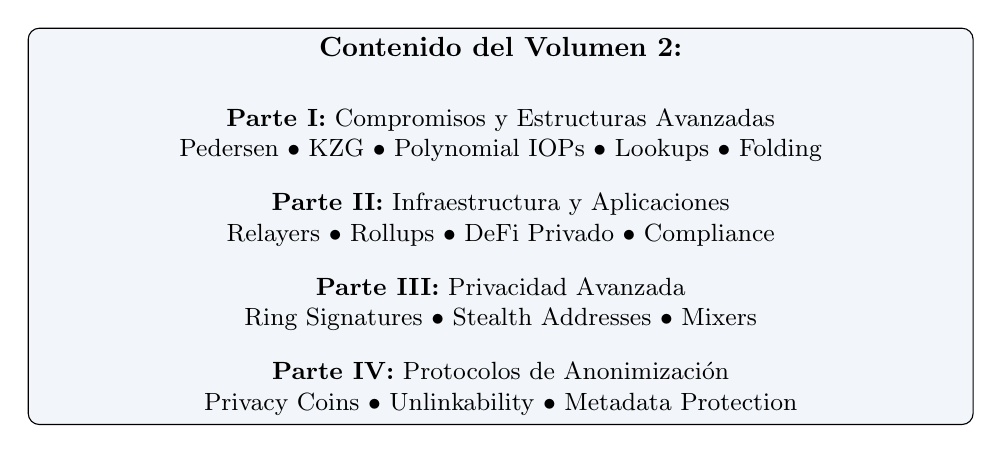
\begin{tikzpicture}
        \node[rectangle, draw, rounded corners, minimum width=12cm, minimum height=5cm, fill=zkblue!5] {
            \begin{minipage}{11cm}
            \centering
            \textbf{Contenido del Volumen 2:}\\[0.5cm]
            \small
            \textbf{Parte I:} Compromisos y Estructuras Avanzadas\\
            Pedersen $\bullet$ KZG $\bullet$ Polynomial IOPs $\bullet$ Lookups $\bullet$ Folding\\[0.3cm]
            \textbf{Parte II:} Infraestructura y Aplicaciones\\
            Relayers $\bullet$ Rollups $\bullet$ DeFi Privado $\bullet$ Compliance\\[0.3cm]
            \textbf{Parte III:} Privacidad Avanzada\\
            Ring Signatures $\bullet$ Stealth Addresses $\bullet$ Mixers\\[0.3cm]
            \textbf{Parte IV:} Protocolos de Anonimizaci\'on\\
            Privacy Coins $\bullet$ Unlinkability $\bullet$ Metadata Protection
            \end{minipage}
        };
    \end{tikzpicture}
    
    \vfill
    
    {\Large Walter Milstein}\\[0.5cm]
    {\large 2025}
\end{titlepage}
% ============================================
% P\'AGINA DE COPYRIGHT
% ============================================
\thispagestyle{empty}
\null\vfill
\begin{center}
\textbf{Banco ZK: Criptograf\'ia y Privacidad en Blockchain}\\
\textbf{Volumen 2: Aplicaciones y Privacidad}\\[1cm]
\textcopyright\ 2025 Walter Milstein\\
Todos los derechos reservados.\\[0.5cm]
Primera Edici\'on: 2025\\[1cm]
\textbf{Serie completa:}\\
Volumen 1: Fundamentos Te\'oricos (Caps. 1--5)\\
Volumen 2: Aplicaciones y Privacidad (Caps. 6--13)\\
Volumen 3: Herramientas Avanzadas y Ecosistema (Caps. 14--20)\\[1cm]
El c\'odigo incluido es de dominio p\'ublico y puede ser utilizado libremente.\\
Este libro es para uso personal y educativo.
\end{center}
\vfill
\cleardoublepage





% ============================================
% DEDICATORIA
% ============================================
\thispagestyle{empty}
\null\vfill
\begin{flushright}
\textit{\large In memoriam Hackeris Euleri, Iacobi Rossini,\\[0.3cm]
ingenii cogitantis architecti,\\
veritatis technicae indefessi inquisitoris,\\
qui codicem non solum ut seriem praeceptorum intellexit,\\
sed ut formam ethicae, rigoris atque libertatis.\\[0.5cm]
Aspectus tuus criticus, fortitudo intellectualis\\
et amor scientiae\\
vivunt adhuc\\
in omni systemate recte excogitato\\
et in omni errore tempestive detecto.}
\end{flushright}
\vfill
\cleardoublepage

% ============================================
% PRERREQUISITOS
% ============================================
\chapter*{Prerrequisitos}
\addcontentsline{toc}{chapter}{Prerrequisitos}

Este volumen asume que el lector ha completado o tiene conocimiento equivalente al contenido del \textbf{Volumen 1: Fundamentos Criptogr\'aficos y Circuitos ZK}.

\section*{Conocimientos Requeridos del Volumen 1}

\begin{itemize}[leftmargin=2cm]
    \item[\textbf{Cap. 1}] \textbf{Fundamentos Criptogr\'aficos:} Funciones hash (SHA-256, Keccak, Poseidon), curvas el\'ipticas (secp256k1, BN254, BLS12-381), firmas digitales, Merkle trees, commitment schemes b\'asicos.
    
    \item[\textbf{Cap. 2}] \textbf{Blockchain Base (L1):} Estructura de transacciones, consenso, modelo UTXO vs Account, gas y fees.
    
    \item[\textbf{Cap. 3}] \textbf{Escalabilidad (L2/L3):} State channels, Plasma, Rollups (Optimistic y ZK), data availability.
    
    \item[\textbf{Cap. 4}] \textbf{Zero-Knowledge Proofs (Core):} Definici\'on formal, propiedades (completeness, soundness, zero-knowledge), SNARKs, STARKs, sistemas de prueba.
    
    \item[\textbf{Cap. 5}] \textbf{Circuitos ZK:} R1CS, Plonkish arithmetization, Circom, snarkjs, Halo2, Arkworks, Noir.
\end{itemize}

\section*{Herramientas Recomendadas}

Para seguir los ejemplos de c\'odigo de este volumen:

\begin{center}
\begin{tabular}{ll}
\toprule
\textbf{Herramienta} & \textbf{Versi\'on M\'inima} \\
\midrule
Node.js & 18+ \\
Rust & 1.70+ \\
Circom & 2.1+ \\
snarkjs & 0.7+ \\
Foundry & \'Ultima estable \\
Python & 3.10+ \\
\bottomrule
\end{tabular}
\end{center}

\section*{Referencias Cruzadas}

A lo largo de este volumen, las referencias al Volumen 1 se indican como:
\begin{center}
\fbox{\textbf{Ver Vol. 1, Cap. X, Sec. Y}}
\end{center}

\cleardoublepage

% ============================================
% TABLA DE CONTENIDOS
% ============================================
\tableofcontents
\cleardoublepage

% ============================================
% LISTA DE CAP\'ITULOS DEL VOLUMEN 2
% ============================================
\chapter*{Estructura del Volumen 2}
\addcontentsline{toc}{chapter}{Estructura del Volumen 2}

\begin{center}
{\Large\bfseries Cap\'itulos 6--13}\\[1cm]

\begin{tabular}{clc}
\toprule
\textbf{Cap.} & \textbf{T\'itulo} & \textbf{P\'aginas Est.} \\
\midrule
6 & Compromisos y Estructuras & $\sim$50 \\
7 & Infraestructura ZK & $\sim$45 \\
8 & Privacidad Avanzada & $\sim$45 \\
9 & DeFi y Aplicaciones & $\sim$40 \\
10 & Avanzado e Investigaci\'on & $\sim$40 \\
11 & Protocolos de Anonimizaci\'on & $\sim$45 \\
12 & Monedas Privadas (Privacy Coins) & $\sim$40 \\
13 & T\'ecnicas de Unlinkability & $\sim$42 \\
\midrule
& \textbf{Total Volumen 2} & $\sim$347 \\
\bottomrule
\end{tabular}
\end{center}

\vspace{1cm}

\begin{center}
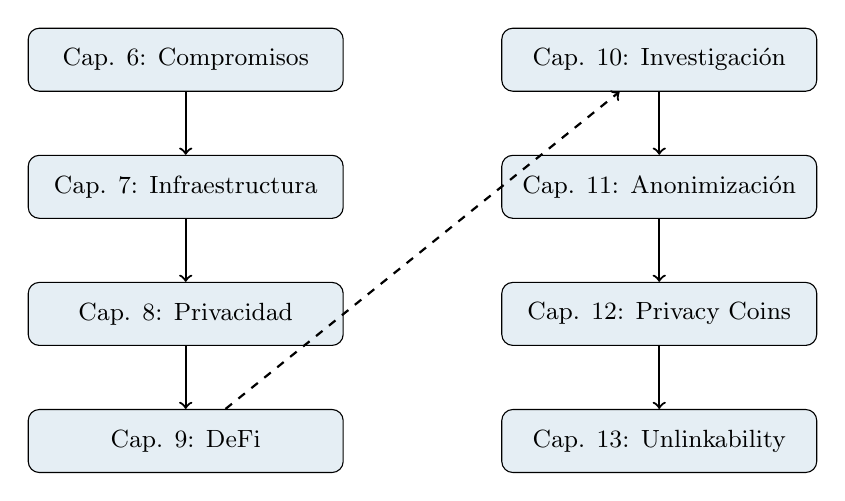
\begin{tikzpicture}[
    node distance=0.8cm,
    box/.style={draw, rectangle, rounded corners, minimum width=4cm, minimum height=0.8cm, fill=zkblue!10, font=\small}
]
    \node[box] (c6) {Cap. 6: Compromisos};
    \node[box, below=of c6] (c7) {Cap. 7: Infraestructura};
    \node[box, below=of c7] (c8) {Cap. 8: Privacidad};
    \node[box, below=of c8] (c9) {Cap. 9: DeFi};
    
    \node[box, right=2cm of c6] (c10) {Cap. 10: Investigaci\'on};
    \node[box, below=of c10] (c11) {Cap. 11: Anonimizaci\'on};
    \node[box, below=of c11] (c12) {Cap. 12: Privacy Coins};
    \node[box, below=of c12] (c13) {Cap. 13: Unlinkability};
    
    \draw[->, thick] (c6) -- (c7);
    \draw[->, thick] (c7) -- (c8);
    \draw[->, thick] (c8) -- (c9);
    \draw[->, thick, dashed] (c9) -- (c10);
    \draw[->, thick] (c10) -- (c11);
    \draw[->, thick] (c11) -- (c12);
    \draw[->, thick] (c12) -- (c13);
\end{tikzpicture}
\end{center}

\cleardoublepage

% ============================================
% CAP\'ITULO 1 (CAP 6 ORIGINAL): COMPROMISOS Y ESTRUCTURAS
% ============================================
\chapter{Compromisos y Estructuras}
\label{ch:compromisos}

\begin{center}
\textit{Cap\'itulo 6 de la serie $\cdot$ Cap\'itulo 1 del Volumen 2}
\end{center}

\vspace{1cm}

%===========================================
\section{Commitment Schemes: Qu\'e son, Para qu\'e sirven}
%===========================================

\begin{definition}[Esquema de Compromiso]
Protocolo criptogr\'afico con dos fases:
\begin{enumerate}
    \item \textbf{Commit:} Sellar un valor
    \item \textbf{Open:} Revelar y verificar
\end{enumerate}
\end{definition}

%-------------------------------------------
\subsection{Intuici\'on y Analog\'ias}

\begin{intuicion}
Un commitment es como un sobre sellado:
\begin{itemize}
    \item Escribes algo en un papel y lo metes en un sobre opaco
    \item Sellas el sobre y lo entregas
    \item Nadie puede ver qu\'e hay dentro (hiding)
    \item No puedes cambiar el contenido sin que se note (binding)
    \item M\'as tarde, abres el sobre para revelar el contenido
\end{itemize}

\textbf{Ejemplos cotidianos:}
\begin{itemize}
    \item \textbf{Subasta sellada:} Cada participante ``compromete'' su oferta en un sobre. Despu\'es de cerrar, todos revelan.
    \item \textbf{Juego piedra-papel-tijera:} Ambos jugadores eligen y ``comprometen'' (mano cerrada), luego revelan simult\'aneamente.
    \item \textbf{Hash como commitment:} ``Mi predicci\'on est\'a en el hash X'' $\to$ luego revelas el texto y verifican que hashea a X.
\end{itemize}
\end{intuicion}

%-------------------------------------------
\subsection{Propiedades Formales}

\begin{definition}[Propiedades de un Commitment Scheme]
Un esquema de compromiso $(C, O)$ sobre espacio de mensajes $\mathcal{M}$ satisface:

\textbf{1. Hiding (Ocultamiento):}
\[ \forall m_0, m_1 \in \mathcal{M}: \text{Commit}(m_0) \approx \text{Commit}(m_1) \]
El compromiso no revela informaci\'on sobre el mensaje.

\textbf{2. Binding (Vinculaci\'on):}
\[ \Pr[\text{Open}(c, m_1, r_1) = 1 \land \text{Open}(c, m_2, r_2) = 1 \land m_1 \neq m_2] \leq \negl(\lambda) \]
No es posible abrir el mismo compromiso a dos mensajes diferentes.
\end{definition}

\begin{mathnote}
\textbf{Tipos de seguridad:}

\begin{center}
\begin{tabular}{lcc}
\toprule
\textbf{Esquema} & \textbf{Hiding} & \textbf{Binding} \\
\midrule
Pedersen & Perfect (info-theoretic) & Computational \\
Hash-based & Computational & Perfect (info-theoretic) \\
ElGamal & Computational & Computational \\
\bottomrule
\end{tabular}
\end{center}

\textbf{Teorema (Imposibilidad):} No puede existir un esquema con hiding perfecto Y binding perfecto simult\'aneamente.

\textbf{Demostraci\'on (intuici\'on):}
\begin{itemize}
    \item Si hiding es perfecto, para cada $c$ existen m\'ultiples $(m, r)$ que lo producen
    \item Esto significa que binding no puede ser perfecto (hay colisiones)
    \item Y viceversa
\end{itemize}
\end{mathnote}

%-------------------------------------------
\subsection{Aplicaciones}

Las aplicaciones principales de los commitment schemes incluyen:
\begin{itemize}
    \item Ocultar valores en transacciones (Confidential Tx)
    \item Comprometer a polinomios (SNARKs)
    \item Voting schemes
    \item Auctions selladas
\end{itemize}

\begin{example}[Aplicaciones detalladas]
\textbf{1. Transacciones Confidenciales:}
\begin{lstlisting}[style=python]
# En lugar de: Transfer(Alice, Bob, 100)
# Publicamos: Transfer(Alice, Bob, Commit(100, r))

# El commitment oculta el monto
# Pero permite verificar que sum(inputs) = sum(outputs)
# Gracias al homomorfismo
\end{lstlisting}

\textbf{2. Voting:}
\begin{lstlisting}[style=python]
# Fase 1 (Commit):
#     Cada votante publica C_i = Commit(voto_i, r_i)
    
# Fase 2 (Reveal):
#     Cada votante revela (voto_i, r_i)
#     Se verifica C_i = Commit(voto_i, r_i)
    
# Fase 3 (Count):
#     Contar votos revelados

# Nadie puede cambiar su voto despues de ver otros
# (binding protege contra esto)
\end{lstlisting}

\textbf{3. SNARKs:}
\begin{lstlisting}[style=python]
# Prover compromete a polinomio p(x):
#     C = Commit(p)
    
# Verifier pide evaluacion en punto aleatorio z:
#     y = p(z)
    
# Prover genera prueba de apertura:
#     pi = Open(C, z, y)
    
# Verifier verifica:
#     Verify(C, z, y, pi) = 1
\end{lstlisting}
\end{example}

%===========================================
\section{Pedersen Commitments}
%===========================================

Propiedades clave de Pedersen (introducido en Vol. 1, Cap. 1):
\begin{itemize}
    \item $C = g^m h^r$
    \item Perfectly hiding
    \item Computationally binding
    \item Homom\'orfico aditivo
\end{itemize}

%-------------------------------------------
\subsection{Construcci\'on Detallada}

\begin{definition}[Pedersen Commitment]
Sea $\G$ un grupo c\'iclico de orden primo $q$, y sean $g, h \in \G$ generadores tales que $\log_g(h)$ es desconocido.

\textbf{Commit:} Para mensaje $m \in \Z_q$ y randomness $r \xleftarrow{\$} \Z_q$:
\[ C = g^m \cdot h^r \]

\textbf{Open:} Revelar $(m, r)$ y verificar $C = g^m \cdot h^r$.
\end{definition}

\begin{mathnote}
\textbf{An\'alisis de seguridad:}

\textbf{Perfect Hiding:}

Para cualquier commitment $C$, y cualquier mensaje $m'$, existe exactamente un $r'$ tal que $C = g^{m'} h^{r'}$:
\[ r' = \log_h(C \cdot g^{-m'}) = \log_h(C) - m' \cdot \log_h(g) \]

Por lo tanto, $C$ no da informaci\'on sobre $m$.

\textbf{Computational Binding:}

Sup\'on que puedes abrir $C$ a dos mensajes:
\[ C = g^{m_1} h^{r_1} = g^{m_2} h^{r_2} \]

Entonces:
\[ g^{m_1 - m_2} = h^{r_2 - r_1} \]
\[ \log_g(h) = \frac{m_1 - m_2}{r_2 - r_1} \]

!`Esto calcula el logaritmo discreto de $h$ base $g$!

Si el DLP es dif\'icil, binding es seguro.
\end{mathnote}

%-------------------------------------------
\subsection{Homomorfismo}

\begin{keyidea}
\textbf{Propiedad homom\'orfica aditiva:}

\[ \Commit(m_1, r_1) \cdot \Commit(m_2, r_2) = \Commit(m_1 + m_2, r_1 + r_2) \]

\textbf{Demostraci\'on:}
\begin{align*}
C_1 \cdot C_2 &= (g^{m_1} h^{r_1}) \cdot (g^{m_2} h^{r_2}) \\
&= g^{m_1 + m_2} \cdot h^{r_1 + r_2} \\
&= \Commit(m_1 + m_2, r_1 + r_2)
\end{align*}

\textbf{Aplicaci\'on: Verificar balance sin revelar montos}

\begin{lstlisting}[style=python]
# Inputs:  C_1 = Commit(100, r1), C_2 = Commit(50, r2)
# Outputs: C_3 = Commit(80, r3), C_4 = Commit(70, r4)

# Verificar: C_1 * C_2 = C_3 * C_4 ?

# g^(100+50) * h^(r1+r2) = g^(80+70) * h^(r3+r4) ?
# g^150 * h^(r1+r2) = g^150 * h^(r3+r4)

# Si r1+r2 = r3+r4, la ecuacion se cumple.
# El verificador no conoce los montos individuales.
\end{lstlisting}
\end{keyidea}

%-------------------------------------------
\subsection{Vector Pedersen Commitments}

\begin{definition}[Vector Pedersen Commitment]
Para vector $\vec{m} = (m_1, \ldots, m_n)$ y generadores $g_1, \ldots, g_n, h$:
\[ C = \prod_{i=1}^{n} g_i^{m_i} \cdot h^r = g_1^{m_1} \cdot g_2^{m_2} \cdots g_n^{m_n} \cdot h^r \]

Permite comprometer a m\'ultiples valores en un solo elemento de grupo.
\end{definition}

\begin{example}[Uso en Bulletproofs]
\begin{lstlisting}[style=python]
# Comprometer a vector de bits para range proof
bits = [1, 0, 1, 1, 0, 0, 1, 0]  # 8 bits

# C = g_0^1 * g_1^0 * g_2^1 * g_3^1 * g_4^0 * g_5^0 * g_6^1 * g_7^0 * h^r

# Un solo punto de curva representa 8 bits
# Verificar propiedades de bits sin revelarlos
\end{lstlisting}
\end{example}

%===========================================
\section{KZG Commitments}
%===========================================

Propiedades clave de KZG (introducido en Vol. 1, Cap. 1):
\begin{itemize}
    \item Compromiso a polinomio
    \item Evaluaci\'on verificable en $O(1)$
    \item Requiere trusted setup
    \item Base de PLONK, Danksharding
\end{itemize}

%-------------------------------------------
\subsection{Construcci\'on Detallada}

\begin{definition}[KZG Polynomial Commitment]
\textbf{Setup:} Elegir $\tau \xleftarrow{\$} \F$ secreto (toxic waste). Generar:
\[ \text{SRS} = (g, g^\tau, g^{\tau^2}, \ldots, g^{\tau^d}, h, h^\tau) \]
donde $g$ genera $\G_1$ y $h$ genera $\G_2$.

\textbf{Commit:} Para polinomio $p(x) = \sum_{i=0}^{d} a_i x^i$:
\[ C = g^{p(\tau)} = \prod_{i=0}^{d} (g^{\tau^i})^{a_i} \]

El prover no conoce $\tau$, solo usa los elementos del SRS.

\textbf{Open (evaluaci\'on):} Para probar que $p(z) = y$:
\begin{enumerate}
    \item Calcular polinomio cociente: $q(x) = \frac{p(x) - y}{x - z}$
    \item Commitment al cociente: $\pi = g^{q(\tau)}$
\end{enumerate}

\textbf{Verify:} Verificar con pairing:
\[ e(C / g^y, h) = e(\pi, h^\tau / h^z) \]

O equivalentemente:
\[ e(C - g^y, h) = e(\pi, h^{\tau - z}) \]
\end{definition}

\begin{mathnote}
\textbf{?`Por qu\'e funciona la verificaci\'on?}

Si $p(z) = y$, entonces $(x - z)$ divide a $p(x) - y$.

Existe $q(x)$ tal que:
\[ p(x) - y = q(x) \cdot (x - z) \]

Evaluando en $\tau$:
\[ p(\tau) - y = q(\tau) \cdot (\tau - z) \]

En el grupo:
\[ g^{p(\tau) - y} = g^{q(\tau) \cdot (\tau - z)} \]

Usando pairings:
\[ e(g^{p(\tau) - y}, h) = e(g^{q(\tau)}, h^{\tau - z}) \]
\[ e(C \cdot g^{-y}, h) = e(\pi, h^\tau \cdot h^{-z}) \]
\end{mathnote}

%-------------------------------------------
\subsection{Propiedades de KZG}

\begin{keyidea}
\textbf{Ventajas de KZG:}

\begin{center}
\begin{tabular}{lc}
\toprule
\textbf{Propiedad} & \textbf{Valor} \\
\midrule
Tama\~no del commitment & 48 bytes (BLS12-381) \\
Tama\~no de prueba de evaluaci\'on & 48 bytes \\
Tiempo de verificaci\'on & 2 pairings (constante) \\
Batch verification & Muy eficiente \\
Homomorfismo & Aditivo \\
\bottomrule
\end{tabular}
\end{center}

\textbf{Desventajas:}
\begin{itemize}
    \item Requiere trusted setup
    \item No es post-quantum
    \item Setup size crece con grado m\'aximo del polinomio
\end{itemize}
\end{keyidea}

%-------------------------------------------
\subsection{Batch Opening}

\begin{example}[Abrir m\'ultiples evaluaciones eficientemente]
\textbf{Problema:} Probar $p(z_1) = y_1, p(z_2) = y_2, \ldots, p(z_k) = y_k$

\textbf{Naive:} $k$ pruebas de 48 bytes cada una = $48k$ bytes

\textbf{Batch:} Una sola prueba agregada

\begin{lstlisting}[style=python]
# Verifier elige random gamma
gamma = hash(C, z_1, y_1, ..., z_k, y_k)

# Prover construye polinomio agregado
I_x = sum(gamma**i * y_i for i in range(k))  # Interpolacion
Z_x = prod((x - z_i) for i in range(k))      # Polinomio de ceros

# Prueba unica
q_x = (p_x - I_x) / Z_x
pi = g ** q_tau

# Tamano: 48 bytes (independiente de k)
\end{lstlisting}
\end{example}

%-------------------------------------------
\subsection{KZG en la Pr\'actica}

\begin{remark}
\textbf{Usos de KZG en producci\'on:}

\textbf{1. PLONK y variantes:}
\begin{itemize}
    \item Commitment a polinomios del circuito
    \item Pruebas de evaluaci\'on en puntos aleatorios
    \item Base de zkSync, Polygon zkEVM, Scroll
\end{itemize}

\textbf{2. Ethereum Danksharding (EIP-4844):}
\begin{itemize}
    \item Blobs son polinomios comprometidos con KZG
    \item Permite data availability sampling
    \item Ceremonia con 140,000+ participantes
\end{itemize}

\textbf{3. Verkle Trees:}
\begin{itemize}
    \item Reemplazo propuesto para Merkle Patricia Tries
    \item Pruebas de membres\'ia mucho m\'as peque\~nas
    \item Usando KZG para commitment a branches
\end{itemize}
\end{remark}

\begin{bancozk}
\textbf{KZG en Banco ZK:}

Usamos KZG para:
\begin{itemize}
    \item Polynomial commitments en nuestros circuitos PLONK
    \item SRS de la ceremonia de Ethereum (m\'axima confianza)
    \item Pruebas de evaluaci\'on para verificaci\'on en L1
\end{itemize}

\textbf{Consideraci\'on:} Aunque KZG no es post-quantum, la transici\'on a alternativas (FRI, IPA) est\'a en nuestro roadmap para cuando sea necesario.
\end{bancozk}

%===========================================
\section{IPA: Inner Product Arguments}
%===========================================

\begin{definition}[Inner Product Argument]
Protocolo para probar que el producto interno de dos vectores $\vec{a}, \vec{b} \in \mathbb{F}^n$ es igual a un valor $c$:
\[ \langle \vec{a}, \vec{b} \rangle = \sum_{i=1}^{n} a_i \cdot b_i = c \]
sin revelar los vectores completos.
\end{definition}

%-------------------------------------------
\subsection{Motivaci\'on: Alternativa a KZG}

\begin{intuicion}
\textbf{?`Por qu\'e IPA?}

KZG tiene una debilidad: requiere \textbf{trusted setup}. Si el ``toxic waste'' $\tau$ se filtra, todo el sistema se rompe.

IPA ofrece una alternativa \textbf{transparente}:
\begin{itemize}
    \item No requiere trusted setup
    \item Solo necesita generadores aleatorios (verificables p\'ublicamente)
    \item Trade-off: verificaci\'on $O(\log n)$ en lugar de $O(1)$
\end{itemize}

\textbf{Comparaci\'on r\'apida:}
\begin{center}
\begin{tabular}{lcc}
\toprule
\textbf{Propiedad} & \textbf{KZG} & \textbf{IPA} \\
\midrule
Trusted setup & S\'i & No \\
Tama\~no prueba & $O(1)$ & $O(\log n)$ \\
Verificaci\'on & $O(1)$ pairings & $O(n)$ o $O(\log n)$* \\
Post-quantum & No & No \\
\bottomrule
\end{tabular}
\end{center}
\small{*Con t\'ecnicas de acumulaci\'on, verificaci\'on amortizada es $O(\log n)$}
\end{intuicion}

%-------------------------------------------
\subsection{Construcci\'on de IPA}

\begin{mathnote}
\textbf{Protocolo IPA (simplificado):}

\textbf{Setup p\'ublico:} Generadores $\vec{G} = (G_1, \ldots, G_n)$, $\vec{H} = (H_1, \ldots, H_n)$, $U$ (todos en $\mathbb{G}$).

\textbf{Commitment:} Para vectores $\vec{a}, \vec{b}$ con producto interno $c$:
\[ P = \langle \vec{a}, \vec{G} \rangle + \langle \vec{b}, \vec{H} \rangle + c \cdot U \]

\textbf{Protocolo recursivo (log n rondas):}

En cada ronda $i$, con vectores de tama\~no $n_i = n/2^i$:

1. Prover calcula:
\begin{align*}
L_i &= \langle \vec{a}_{lo}, \vec{G}_{hi} \rangle + \langle \vec{b}_{hi}, \vec{H}_{lo} \rangle + (a_{lo} \cdot b_{hi}) \cdot U \\
R_i &= \langle \vec{a}_{hi}, \vec{G}_{lo} \rangle + \langle \vec{b}_{lo}, \vec{H}_{hi} \rangle + (a_{hi} \cdot b_{lo}) \cdot U
\end{align*}

2. Verifier env\'ia challenge $x_i \xleftarrow{\$} \mathbb{F}$

3. Prover reduce vectores:
\begin{align*}
\vec{a}' &= \vec{a}_{lo} + x_i \cdot \vec{a}_{hi} \\
\vec{b}' &= \vec{b}_{lo} + x_i^{-1} \cdot \vec{b}_{hi} \\
\vec{G}' &= \vec{G}_{lo} + x_i^{-1} \cdot \vec{G}_{hi} \\
\vec{H}' &= \vec{H}_{lo} + x_i \cdot \vec{H}_{hi}
\end{align*}

4. Repetir hasta que vectores tengan tama\~no 1.

\textbf{Prueba final:} $(L_1, R_1, \ldots, L_{\log n}, R_{\log n}, a, b)$

Tama\~no: $2 \log n$ puntos de curva + 2 escalares $\approx O(\log n)$
\end{mathnote}

%-------------------------------------------
\subsection{De IPA a Polynomial Commitment}

\begin{keyidea}
\textbf{Polynomial commitment con IPA:}

Un polinomio $p(x) = \sum_{i=0}^{d} a_i x^i$ se puede ver como vector de coeficientes $\vec{a} = (a_0, \ldots, a_d)$.

Para probar $p(z) = y$:
\begin{enumerate}
    \item Sea $\vec{b} = (1, z, z^2, \ldots, z^d)$
    \item Notar que $\langle \vec{a}, \vec{b} \rangle = p(z) = y$
    \item Usar IPA para probar el producto interno
\end{enumerate}

\textbf{Ventaja:} El verifier conoce $\vec{b}$ (es p\'ublico), as\'i que solo necesita commitment a $\vec{a}$.
\end{keyidea}

%-------------------------------------------
\subsection{Bulletproofs}

\begin{definition}[Bulletproofs]
Sistema de pruebas de rango (range proofs) basado en IPA, con tama\~no $O(\log n)$ sin trusted setup.
\end{definition}

\begin{example}[Range Proof con Bulletproofs]
\textbf{Problema:} Probar que $v \in [0, 2^n)$ sin revelar $v$.

\textbf{Idea:}
\begin{lstlisting}[style=python]
# v en binario: v = sum(a_i * 2^i) donde a_i in {0,1}

# Constraints:
# 1. a_i * (a_i - 1) = 0  (cada a_i es bit)
# 2. sum(a_i * 2^i) = v   (reconstruccion)

# Esto se codifica como producto interno:
# <a, 2^n> = v
# <a, a-1> = 0  (vector-wise)

# IPA prueba ambas condiciones en O(log n)
\end{lstlisting}

\textbf{Tama\~nos (64-bit range proof):}
\begin{center}
\begin{tabular}{lc}
\toprule
\textbf{Esquema} & \textbf{Tama\~no} \\
\midrule
Naive (64 firmas) & $\sim$2 KB \\
Borromean (Monero antiguo) & $\sim$6 KB \\
Bulletproofs & $\sim$700 bytes \\
Bulletproofs+ & $\sim$600 bytes \\
\bottomrule
\end{tabular}
\end{center}
\end{example}

\begin{remark}
\textbf{Usos de IPA/Bulletproofs en producci\'on:}

\begin{itemize}
    \item \textbf{Monero:} Range proofs para transacciones confidenciales
    \item \textbf{Grin/MimbleWimble:} Toda la criptograf\'ia de transacciones
    \item \textbf{Halo/Halo2:} Polynomial commitment scheme (recursi\'on sin pairings)
    \item \textbf{Zcash Orchard:} Migraci\'on de Groth16 a Halo2
\end{itemize}
\end{remark}

%-------------------------------------------
\subsection{Comparaci\'on: KZG vs IPA vs FRI}

\begin{center}
\begin{tabular}{lccc}
\toprule
\textbf{Propiedad} & \textbf{KZG} & \textbf{IPA} & \textbf{FRI} \\
\midrule
Trusted setup & S\'i & No & No \\
Tama\~no prueba & $O(1)$ & $O(\log n)$ & $O(\log^2 n)$ \\
Verificaci\'on & 2 pairings & $O(n)$ & $O(\log^2 n)$ \\
Prover time & $O(n)$ & $O(n)$ & $O(n \log n)$ \\
Post-quantum & No & No & S\'i \\
Assunci\'on & DLP + pairing & DLP & Hash \\
\bottomrule
\end{tabular}
\end{center}

\begin{bancozk}
\textbf{Elecci\'on de PCS en Banco ZK:}

Usamos \textbf{KZG} como PCS principal por:
\begin{itemize}
    \item Verificaci\'on $O(1)$ cr\'itica para L1 (gas costs)
    \item Trusted setup de Ethereum (140K+ participantes)
    \item Compatibilidad con ecosistema existente
\end{itemize}

\textbf{Plan de migraci\'on:}
\begin{itemize}
    \item Corto plazo: KZG (producci\'on actual)
    \item Mediano plazo: Halo2/IPA (eliminar trusted setup)
    \item Largo plazo: FRI/STARKs (post-quantum)
\end{itemize}

La arquitectura modular (PIOP + PCS separados) permite cambiar el PCS sin reescribir los circuitos.
\end{bancozk}

%===========================================
\section{Polynomial IOPs}
%===========================================

\begin{definition}[Polynomial IOP]
Protocolo interactivo donde el prover env\'ia polinomios (comprometidos) y el verifier hace queries.
\end{definition}

Estructura t\'ipica:
\begin{enumerate}
    \item Prover compromete a polinomios que codifican el witness
    \item Verifier env\'ia challenges aleatorios
    \item Prover abre evaluaciones en puntos espec\'ificos
    \item Verifier chequea relaciones polinomiales
\end{enumerate}

%-------------------------------------------
\subsection{Entendiendo Polynomial IOPs}

\begin{intuicion}
\textbf{?`Por qu\'e polinomios?}

Los polinomios tienen una propiedad m\'agica: el \textbf{Schwartz-Zippel Lemma}.

\textbf{Lemma:} Si $p(x)$ es un polinomio no-cero de grado $d$ sobre campo $\F$, entonces:
\[ \Pr_{r \xleftarrow{\$} \F}[p(r) = 0] \leq \frac{d}{|\F|} \]

Para campos grandes ($|\F| \approx 2^{256}$) y grados peque\~nos ($d \approx 10^6$):
\[ \Pr \leq \frac{10^6}{2^{256}} \approx 0 \]

\textbf{Implicaci\'on:} Si dos polinomios $p(x)$ y $q(x)$ de grado $d$ coinciden en un punto aleatorio, son iguales con probabilidad abrumadora.

Esto permite verificar identidades polinomiales con UN SOLO punto.
\end{intuicion}

\begin{mathnote}
\textbf{De constraints a polinomios:}

\textbf{Paso 1: Codificar constraints como polinomio}

Un circuito con $n$ constraints:
\[ C_1(w), C_2(w), \ldots, C_n(w) \]

Se codifica como polinomio $T(X)$ que es cero en puntos $\omega^0, \omega^1, \ldots, \omega^{n-1}$:
\[ T(\omega^i) = 0 \iff C_i(w) \text{ se satisface} \]

\textbf{Paso 2: Verificar con vanishing polynomial}

Si $T(X)$ es cero en todos los $\omega^i$, entonces $Z_H(X) = \prod_{i=0}^{n-1}(X - \omega^i)$ divide a $T(X)$.

Existe $Q(X)$ tal que:
\[ T(X) = Q(X) \cdot Z_H(X) \]

\textbf{Paso 3: Verificaci\'on en punto aleatorio}

Verifier elige $\zeta$ aleatorio y verifica:
\[ T(\zeta) = Q(\zeta) \cdot Z_H(\zeta) \]

Si esto se cumple, con alta probabilidad $T(X)$ es divisible por $Z_H(X)$, lo que significa que todos los constraints se satisfacen.
\end{mathnote}

%-------------------------------------------
\subsection{Estructura de un SNARK Moderno}

SNARKs modernos = Polynomial IOP + Polynomial Commitment:
\begin{itemize}
    \item PLONK = PIOP + KZG
    \item Halo2 = PIOP + IPA
    \item STARKs = PIOP + FRI
\end{itemize}

\begin{center}
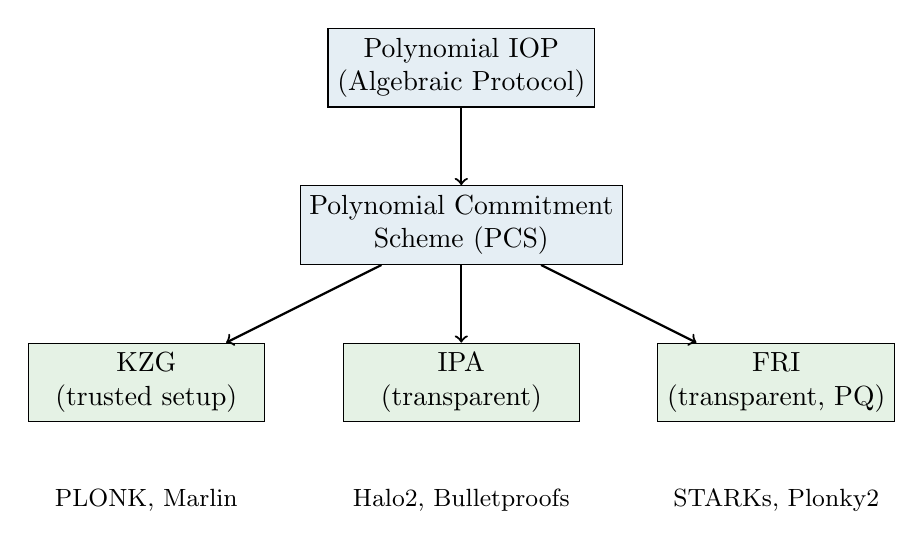
\begin{tikzpicture}[
    box/.style={draw, rectangle, minimum width=3cm, minimum height=1cm, align=center, fill=zkblue!10},
    arrow/.style={->, thick}
]
    % Layers
    \node[box] (piop) at (0, 2) {Polynomial IOP\\(Algebraic Protocol)};
    \node[box] (pcs) at (0, 0) {Polynomial Commitment\\Scheme (PCS)};
    
    \node[box, fill=zkgreen!10] (kzg) at (-4, -2) {KZG\\(trusted setup)};
    \node[box, fill=zkgreen!10] (ipa) at (0, -2) {IPA\\(transparent)};
    \node[box, fill=zkgreen!10] (fri) at (4, -2) {FRI\\(transparent, PQ)};
    
    % Arrows
    \draw[arrow] (piop) -- (pcs);
    \draw[arrow] (pcs) -- (kzg);
    \draw[arrow] (pcs) -- (ipa);
    \draw[arrow] (pcs) -- (fri);
    
    % Labels
    \node at (-4, -3.5) {\small PLONK, Marlin};
    \node at (0, -3.5) {\small Halo2, Bulletproofs};
    \node at (4, -3.5) {\small STARKs, Plonky2};
\end{tikzpicture}
\end{center}

\begin{keyidea}
\textbf{Separaci\'on de concerns:}

\textbf{Polynomial IOP} define:
\begin{itemize}
    \item Qu\'e polinomios env\'ia el prover
    \item Qu\'e relaciones deben satisfacer
    \item Qu\'e queries hace el verifier
\end{itemize}

\textbf{Polynomial Commitment Scheme} define:
\begin{itemize}
    \item C\'omo comprometer a polinomios
    \item C\'omo probar evaluaciones
    \item Propiedades de seguridad
\end{itemize}

Esta separaci\'on permite:
\begin{itemize}
    \item Cambiar el PCS sin cambiar el PIOP
    \item Optimizar cada parte independientemente
    \item Elegir trade-offs (setup, tama\~no, velocidad)
\end{itemize}
\end{keyidea}

%-------------------------------------------
\subsection{Ejemplo: PLONK como Polynomial IOP}

\begin{example}[PLONK simplificado]
\textbf{Setup:}
\begin{itemize}
    \item Dominio $H = \{\omega^0, \omega^1, \ldots, \omega^{n-1}\}$ donde $\omega^n = 1$
    \item Polinomios selectores $q_L, q_R, q_O, q_M, q_C$ (fijos)
    \item Polinomio de permutaci\'on $\sigma$ (fijo)
\end{itemize}

\textbf{Prover env\'ia:}
\begin{enumerate}
    \item Commitments a $a(X), b(X), c(X)$ (valores de wires)
    \item Commitment a $z(X)$ (acumulador de permutaci\'on)
    \item Commitments a polinomios cocientes $t(X)$
\end{enumerate}

\textbf{Verifier queries:}
\begin{itemize}
    \item Punto aleatorio $\zeta$
    \item Evaluaciones: $a(\zeta), b(\zeta), c(\zeta), z(\zeta), z(\omega\zeta), \ldots$
\end{itemize}

\textbf{Verificaci\'on:}
\begin{enumerate}
    \item Gate constraint:
    \[ q_L(\zeta) \cdot a(\zeta) + q_R(\zeta) \cdot b(\zeta) + q_O(\zeta) \cdot c(\zeta) + q_M(\zeta) \cdot a(\zeta) \cdot b(\zeta) + q_C(\zeta) = t(\zeta) \cdot Z_H(\zeta) \]
    
    \item Permutation constraint: (m\'as complejo, involucra $z(X)$)
\end{enumerate}
\end{example}

%===========================================
\section{Lookup Arguments (Plookup)}
%===========================================

\begin{definition}[Lookup Argument]
Prueba de que un conjunto de valores est\'a contenido en una tabla.
\end{definition}

%-------------------------------------------
\subsection{Motivaci\'on}

\begin{intuicion}
\textbf{?`Por qu\'e necesitamos lookups?}

Algunas operaciones son dif\'iciles de expresar como polinomios de grado bajo:
\begin{itemize}
    \item XOR de bits: $a \oplus b$ no es algebraico
    \item Comparaciones: $a < b$ requiere descomposici\'on en bits
    \item Funciones arbitrarias: S-boxes de AES, SHA
\end{itemize}

\textbf{Soluci\'on:} Si la funci\'on tiene dominio peque\~no, podemos tabularla.

\textbf{Ejemplo XOR de 8 bits:}
\begin{lstlisting}[style=python]
# Tabla T con 256 x 256 = 65536 entradas:
# | a   | b   | a XOR b |
# |-----|-----|---------|
# | 0   | 0   |    0    |
# | 0   | 1   |    1    |
# | ...
# | 255 | 255 |    0    |

# Probar: (5, 3, 6) in T  (porque 5 XOR 3 = 6)
\end{lstlisting}

En lugar de constraints complicados, simplemente probamos que $(a, b, c)$ est\'a en la tabla.
\end{intuicion}

%-------------------------------------------
\subsection{Protocolo Plookup}

Dado:
\begin{itemize}
    \item Tabla $t = (t_1, \ldots, t_n)$
    \item Valores a verificar $f = (f_1, \ldots, f_m)$
\end{itemize}

Probar: $\forall i: f_i \in \{t_1, \ldots, t_n\}$

Idea:
\begin{enumerate}
    \item Ordenar $f$ y $t$ juntos
    \item Construir polinomio que relaciona listas ordenadas
    \item Verificar con permutation argument
\end{enumerate}

\begin{mathnote}
\textbf{Plookup en detalle:}

\textbf{Observaci\'on clave:}

Si $f$ est\'a contenido en $t$, podemos construir una lista $s$ que es:
\begin{itemize}
    \item Una permutaci\'on de $t$ con elementos de $f$ intercalados
    \item Ordenada de la misma forma que $t$
\end{itemize}

\textbf{Construcci\'on:}

Sea $s = \text{sort}(f \cup t)$ donde cada elemento de $f$ se coloca junto a su correspondiente en $t$.

\textbf{Propiedad:} Para elementos consecutivos en $s$:
\[ s_i = s_{i+1} \quad \text{o} \quad (s_i, s_{i+1}) \in \{(t_j, t_{j+1})\} \]

Esta propiedad se verifica con un grand product.

\textbf{Grand Product:}

\[ \prod_{i} \frac{(1 + \beta)(t_i + \gamma)(t_{i+1} + \gamma)}{(s_i + \gamma)(s_{i+1} + \gamma)} = 1 \]

Si esta igualdad se cumple para $\beta, \gamma$ aleatorios, con alta probabilidad $f \subseteq t$.
\end{mathnote}

\begin{example}[Plookup ilustrado]
\begin{lstlisting}[style=python]
# Tabla t = [1, 2, 3, 4, 5]
# Valores f = [2, 4, 2]

# Paso 1: Verificar que cada f_i esta en t
# - 2 in t: OK
# - 4 in t: OK
# - 2 in t: OK

# Paso 2: Construir s = sort(f U t)
s = [1, 2, 2, 2, 3, 4, 4, 5]
#    ^  ^  ^  ^  ^  ^  ^  ^
#    t  t  f  f  t  t  f  t

# Paso 3: Verificar propiedad de consecutivos
# - (1,2): diferencia de 1 en t OK
# - (2,2): iguales OK
# - (2,2): iguales OK
# - (2,3): diferencia de 1 en t OK
# - (3,4): diferencia de 1 en t OK
# - (4,4): iguales OK
# - (4,5): diferencia de 1 en t OK

# Paso 4: Grand product con random beta, gamma
# (calculo algebraico que verifica todo a la vez)
\end{lstlisting}
\end{example}

%-------------------------------------------
\subsection{Aplicaciones de Lookups}

Aplicaciones principales:
\begin{itemize}
    \item Range proofs eficientes
    \item Operaciones de bits (XOR, AND)
    \item S-boxes en hashes
    \item Cualquier funci\'on tabulable
\end{itemize}

\begin{example}[Range proof con lookup]
\textbf{Sin lookup (descomposici\'on en bits):}
\begin{lstlisting}[style=python]
# Probar x in [0, 2^16)
# Descomponer en 16 bits: 16 constraints
# Verificar cada bit es 0 o 1: 16 constraints
# Reconstruir: 1 constraint
# Total: ~33 constraints
\end{lstlisting}

\textbf{Con lookup:}
\begin{lstlisting}[style=python]
# Tabla T = [0, 1, 2, ..., 65535]
# Probar x in T: ~1 constraint (amortizado)
# Total: ~1 constraint
\end{lstlisting}

\textbf{Para rangos m\'as grandes:}
\begin{lstlisting}[style=python]
# Probar x in [0, 2^32)
# Descomponer x = x_hi * 2^16 + x_lo
# Lookup x_hi in [0, 2^16)
# Lookup x_lo in [0, 2^16)
# Total: ~2 constraints (vs ~65 sin lookup)
\end{lstlisting}
\end{example}

\begin{example}[Operaciones de bits]
\begin{lstlisting}[style=python]
# Tabla XOR de 4 bits (256 entradas)
XOR_TABLE = [(a, b, a^b) for a in range(16) for b in range(16)]

# Para calcular x XOR y donde x, y son de 8 bits:
x_lo, x_hi = x % 16, x // 16
y_lo, y_hi = y % 16, y // 16

# 4 lookups:
# lookup(x_lo, y_lo, z_lo) in XOR_TABLE
# lookup(x_hi, y_hi, z_hi) in XOR_TABLE

z = z_lo + 16 * z_hi

# Total: 4 lookups (~4 constraints) vs ~32 constraints naive
\end{lstlisting}
\end{example}

%-------------------------------------------
\subsection{Variantes de Lookup Arguments}

\begin{remark}
\textbf{Evoluci\'on de lookup arguments:}

\begin{center}
\begin{tabular}{lccc}
\toprule
\textbf{Esquema} & \textbf{A\~no} & \textbf{Costo} & \textbf{Caracter\'istica} \\
\midrule
Plookup & 2020 & $O(n)$ & Original \\
Caulk & 2022 & $O(m \log m)$ & Sublineal en tabla \\
Caulk+ & 2022 & Mejorado & Optimizaciones \\
Baloo & 2022 & $O(m)$ & M\'as simple \\
Lasso/Jolt & 2023 & $O(m \log m)$ & Para zkVM \\
\bottomrule
\end{tabular}
\end{center}

\textbf{Tendencia:} Hacia lookups m\'as eficientes para tablas muy grandes (necesarios para zkVMs).
\end{remark}

\begin{bancozk}
\textbf{Lookups en Banco ZK:}

\textbf{Usamos lookups para:}
\begin{itemize}
    \item Range checks de montos (asegurar $0 \leq \text{amount} < 2^{64}$)
    \item Verificaci\'on de \'indices de Merkle tree
    \item Optimizaci\'on de operaciones de Poseidon (S-box)
\end{itemize}

\textbf{Tablas predefinidas:}
\begin{lstlisting}[style=python]
RANGE_16 = list(range(65536))           # Para range checks
POSEIDON_SBOX = [(x, x**5) for x in F]  # Para S-box
MERKLE_DEPTH = list(range(32))          # Para indices de profundidad
\end{lstlisting}

\textbf{Beneficio:} Circuitos 3-5x m\'as peque\~nos que sin lookups.
\end{bancozk}

%===========================================
\section{Accumulation Schemes}
%===========================================

\begin{definition}[Accumulation]
Combinar m\'ultiples instancias en una sola, difiriendo verificaci\'on.
\end{definition}

En lugar de verificar $n$ pruebas:
\begin{enumerate}
    \item Acumular en un ``acumulador''
    \item Verificar el acumulador una vez al final
    \item Costo: verificaci\'on de 1 prueba, no $n$
\end{enumerate}

%-------------------------------------------
\subsection{Motivaci\'on}

\begin{intuicion}
\textbf{El problema de verificar muchas pruebas:}

Imagina un rollup que procesa 10,000 transacciones:
\begin{itemize}
    \item Cada tx tiene una prueba ZK individual
    \item Verificar cada prueba: $\sim$200K gas
    \item Total naive: $10,000 \times 200K = 2$ mil millones de gas (!`imposible!)
\end{itemize}

\textbf{Soluci\'on 1: Proof Aggregation}
\begin{itemize}
    \item Generar una prueba que verifica las 10,000 pruebas
    \item Problema: verificar pruebas dentro de circuito es MUY caro
    \item Un pairing en circuito $\approx$ millones de constraints
\end{itemize}

\textbf{Soluci\'on 2: Accumulation}
\begin{itemize}
    \item No verificar completamente cada prueba
    \item ``Acumular'' la verificaci\'on pendiente
    \item Al final, una sola verificaci\'on completa
    \item Costo por prueba: casi nada
\end{itemize}
\end{intuicion}

%-------------------------------------------
\subsection{C\'omo Funciona la Acumulaci\'on}

\begin{mathnote}
\textbf{Esquema de acumulaci\'on:}

\textbf{Setup:}
\begin{itemize}
    \item Sistema SNARK con verificaci\'on $V(\text{vk}, x, \pi) \to \{0, 1\}$
    \item Acumulador inicial $\text{acc}_0$
\end{itemize}

\textbf{Acumulaci\'on:}

Para cada nueva prueba $\pi_i$:
\[ \text{acc}_{i+1} = \text{Accumulate}(\text{acc}_i, x_i, \pi_i) \]

El acumulador ``absorbe'' la prueba sin verificarla completamente.

\textbf{Verificaci\'on diferida:}

Al final:
\[ \text{DeciderVerify}(\text{acc}_n) \to \{0, 1\} \]

Si acepta, TODAS las pruebas acumuladas eran v\'alidas.

\textbf{Propiedad clave:}
\[ \text{DeciderVerify}(\text{acc}_n) = 1 \iff \forall i: V(\text{vk}, x_i, \pi_i) = 1 \]
\end{mathnote}

\begin{example}[Acumulaci\'on en Halo]
\begin{lstlisting}[style=python]
# Sistema IPA (Inner Product Argument)
# Verificacion normal: O(n) operaciones de grupo

# Con acumulacion:
acc = initial_accumulator()

for i in range(1000):
    proof_i = receive_proof()
    
    # Acumular: O(1) operaciones
    acc = accumulate(acc, proof_i)
    
    # NO verificamos completamente aqui

# Al final: UNA verificacion O(n)
final_check = decider_verify(acc)

# Costo total:
# - 1000 acumulaciones O(1): ~1000 ops
# - 1 verificacion final O(n): ~n ops
# vs naive: 1000 verificaciones O(n) = 1000n ops
\end{lstlisting}
\end{example}

%===========================================
\section{Recursi\'on de Pruebas}
%===========================================

\begin{definition}[Prueba Recursiva]
Prueba que verifica otra prueba dentro de un circuito.
\end{definition}

%-------------------------------------------
\subsection{Desaf\'ios}

\begin{itemize}
    \item Verificar pairings en circuito es muy costoso
    \item Campo del circuito $\neq$ campo de la curva verificada
    \item Soluci\'on: cycles de curvas
\end{itemize}

\begin{mathnote}
\textbf{El problema de los campos:}

\textbf{Situaci\'on:}
\begin{itemize}
    \item SNARK sobre curva $E_1$ trabaja en campo $\F_{p_1}$ (campo base)
    \item El circuito opera en campo $\F_{r_1}$ (campo escalar)
    \item Para verificar dentro del circuito, necesitamos aritm\'etica de $\F_{p_1}$ en $\F_{r_1}$
\end{itemize}

\textbf{Problema:}

Si $p_1 \neq r_1$ (lo normal), cada operaci\'on de campo requiere:
\begin{itemize}
    \item Aritm\'etica de enteros grandes
    \item Modular reduction
    \item Muchos constraints
\end{itemize}

Una multiplicaci\'on de campo: $\sim$100 constraints

Un pairing: $\sim$millones de constraints

\textbf{Soluci\'on: 2-cycle de curvas}

Curvas $E_1$ y $E_2$ tales que:
\begin{itemize}
    \item Campo base de $E_1$ = Campo escalar de $E_2$: $p_1 = r_2$
    \item Campo escalar de $E_1$ = Campo base de $E_2$: $r_1 = p_2$
\end{itemize}

Ahora:
\begin{itemize}
    \item Prueba sobre $E_1$ se verifica ``nativamente'' en circuito sobre $E_2$
    \item Prueba sobre $E_2$ se verifica ``nativamente'' en circuito sobre $E_1$
    \item Alternamos entre las dos curvas
\end{itemize}
\end{mathnote}

\begin{example}[Pasta Curves (Pallas y Vesta)]
\begin{lstlisting}[style=python]
# Pallas: y^2 = x^3 + 5
#     Base field:   p = 0x40000000...01
#     Scalar field: q = 0x40000000...01 (diferente)

# Vesta: y^2 = x^3 + 5  (misma ecuacion, diferentes campos)
#     Base field:   q (= scalar de Pallas)
#     Scalar field: p (= base de Pallas)

# Uso en recursion:
# 1. Prueba pi_1 sobre Pallas (circuito en F_q)
# 2. Prueba pi_2 sobre Vesta verifica pi_1 (circuito en F_p)
# 3. Prueba pi_3 sobre Pallas verifica pi_2 (circuito en F_q)
# 4. ...alternando...

# Cada verificacion es ''nativa'' - no hay overhead de 
# aritmetica de campo grande.
\end{lstlisting}

Usados por: Mina Protocol, Halo2
\end{example}

%-------------------------------------------
\subsection{Aplicaciones de Recursi\'on}

\begin{itemize}
    \item \textbf{Proof aggregation:} $n$ pruebas $\to$ 1 prueba
    \item \textbf{IVC:} Computaci\'on incremental verificable
    \item \textbf{Rollups:} Miles de txs comprimidas
    \item \textbf{Blockchains sucintas:} Mina (22 KB siempre)
\end{itemize}

\begin{example}[Aplicaciones detalladas de recursi\'on]
\textbf{1. Proof Aggregation para Rollups:}
\begin{lstlisting}[style=python]
# 10,000 transacciones, cada una con proof individual
proofs = [pi_1, pi_2, ..., pi_10000]

# Arbol de agregacion (log depth)
# Level 0: 10,000 proofs
# Level 1: 5,000 proofs (cada uno verifica 2)
# Level 2: 2,500 proofs
# ...
# Level 13: 1 proof final

# La prueba final:
# - Verifica todas las 10,000 transacciones
# - Tamano: ~200-500 bytes
# - Verificacion en L1: ~200K gas
\end{lstlisting}

\textbf{2. Incremental Verifiable Computation (IVC):}
\begin{lstlisting}[style=python]
# Computacion larga: F aplicada 1 millon de veces
# F(F(F(...F(x)...))) = y

# Sin IVC: guardar todo el trace (1M estados)
# Con IVC:

state = x
proof = trivial_proof()

for i in range(1_000_000):
    new_state = F(state)
    proof = prove(
        statement=''new_state = F(state) AND proof_prev is valid'',
        witness=(state, new_state, proof)
    )
    state = new_state

# proof final prueba toda la computacion
# Tamano constante, independiente de 1M pasos
\end{lstlisting}

\textbf{3. Mina Protocol (Blockchain Sucinta):}
\begin{lstlisting}[style=python]
# Blockchain tradicional: verificar = descargar todo
# Bitcoin: ~500 GB
# Ethereum: ~1 TB+

# Mina: siempre 22 KB

# Cada bloque contiene:
# - Transacciones del bloque
# - Proof recursivo que verifica:
#   - Bloque anterior era valido
#   - Nuevas transacciones son validas
#   - Estado se actualizo correctamente

# Verificar toda la blockchain = verificar 1 proof
\end{lstlisting}
\end{example}

%===========================================
\section{Folding Schemes (Nova, Supernova)}
%===========================================

\begin{definition}[Folding]
Combinar dos instancias de un circuito en una, sin generar prueba completa.
\end{definition}

%-------------------------------------------
\subsection{La Innovaci\'on de Folding}

\begin{intuicion}
\textbf{Folding vs Recursi\'on tradicional:}

\textbf{Recursi\'on tradicional:}
\begin{itemize}
    \item Genera prueba completa en cada paso
    \item Verifica prueba anterior dentro del circuito
    \item Costoso: circuito de verificaci\'on es grande
\end{itemize}

\textbf{Folding:}
\begin{itemize}
    \item NO genera prueba en cada paso
    \item ``Combina'' dos instancias en una
    \item Solo al FINAL genera una prueba SNARK
    \item Muy barato por paso
\end{itemize}

\textbf{Analog\'ia:}
\begin{itemize}
    \item Recursi\'on = hacer examen completo en cada clase
    \item Folding = tomar notas en cada clase, examen final al terminar el curso
\end{itemize}
\end{intuicion}

%-------------------------------------------
\subsection{Nova}

Caracter\'isticas de Nova:
\begin{itemize}
    \item Folding para R1CS
    \item Overhead m\'inimo por paso: 2 multiplicaciones de grupo
    \item Solo genera prueba SNARK al final
    \item Ideal para IVC
\end{itemize}

Proceso:
\begin{enumerate}
    \item Instancia 1: $(u_1, w_1)$
    \item Instancia 2: $(u_2, w_2)$
    \item Fold: $(u', w') = \text{Fold}((u_1, w_1), (u_2, w_2), r)$
    \item $u'$ es ``running instance''
    \item Al final: SNARK sobre $u'$
\end{enumerate}

\begin{mathnote}
\textbf{Nova en detalle:}

\textbf{Relaxed R1CS:}

R1CS normal: $Az \circ Bz = Cz$

Nova usa ``relaxed R1CS'':
\[ Az \circ Bz = u \cdot Cz + E \]

Donde:
\begin{itemize}
    \item $u$ es un escalar (1 para instancia normal)
    \item $E$ es un vector de ``error''
\end{itemize}

Para instancia satisfecha normal: $u = 1$, $E = \vec{0}$.

\textbf{Folding de dos instancias:}

Dadas:
\begin{itemize}
    \item $(u_1, E_1, w_1)$ satisfaciendo $A w_1 \circ B w_1 = u_1 C w_1 + E_1$
    \item $(u_2, E_2, w_2)$ satisfaciendo $A w_2 \circ B w_2 = u_2 C w_2 + E_2$
\end{itemize}

Fold con random $r$:
\begin{align*}
u' &= u_1 + r \cdot u_2 \\
w' &= w_1 + r \cdot w_2 \\
E' &= E_1 + r \cdot T + r^2 \cdot E_2
\end{align*}

Donde $T$ es un ``cross term'' calculado por el prover.

\textbf{Propiedad m\'agica:}

$(u', E', w')$ satisface relaxed R1CS si y solo si ambas instancias originales lo satisfac\'ian.

\textbf{Costo del fold:}
\begin{itemize}
    \item Prover: calcular $T$, 1 commitment
    \item Verifier: 2 multiplicaciones escalares de grupo
    \item !`Sin verificaci\'on de SNARK!
\end{itemize}
\end{mathnote}

\begin{example}[IVC con Nova]
\begin{lstlisting}[style=rust]
// Funcion a iterar
fn F(state: State) -> State {
    // Alguna computacion
}

// IVC con Nova
fn nova_ivc(initial_state: State, n: usize) -> (State, Proof) {
    // Inicializar
    let mut running_instance = trivial_instance();
    let mut state = initial_state;
    
    for i in 0..n {
        // Calcular siguiente estado
        let new_state = F(state);
        
        // Crear instancia para este paso
        let step_instance = create_instance(state, new_state);
        
        // Fold (muy barato!)
        running_instance = fold(running_instance, step_instance);
        
        state = new_state;
    }
    
    // Solo al final: generar SNARK
    let proof = spartan_prove(running_instance);
    
    return (state, proof);
}

// Costos:
// - Cada fold: ~10us
// - SNARK final: ~100ms
// - 1 millon de pasos: ~10s (vs dias con recursion tradicional)
\end{lstlisting}
\end{example}

%-------------------------------------------
\subsection{Supernova}

Extensi\'on de Nova para circuitos heterog\'eneos.

\begin{itemize}
    \item Permite alternar entre diferentes circuitos
    \item Selector de cu\'al circuito ejecutar
    \item \'Util para VMs y computaci\'on general
\end{itemize}

\begin{keyidea}
\textbf{Nova vs Supernova:}

\textbf{Nova:}
\begin{itemize}
    \item Un circuito $F$
    \item Ejecutar: $F, F, F, F, \ldots$ (siempre el mismo)
    \item Ideal para: hash chains, funciones recursivas simples
\end{itemize}

\textbf{Supernova:}
\begin{itemize}
    \item M\'ultiples circuitos $F_1, F_2, \ldots, F_k$
    \item Ejecutar: $F_2, F_1, F_3, F_1, F_2, \ldots$ (cualquier orden)
    \item Selector indica cu\'al ejecutar en cada paso
    \item Ideal para: VMs, computaci\'on general
\end{itemize}

\textbf{Ejemplo VM:}
\begin{lstlisting}[style=python]
# Circuitos:
F_1 = ''ADD instruction''
F_2 = ''MUL instruction''
F_3 = ''LOAD instruction''
F_4 = ''STORE instruction''
F_5 = ''JUMP instruction''

# Ejecucion:
# LOAD, ADD, MUL, STORE, JUMP, LOAD, ...
#   F_3,  F_1,  F_2,   F_4,  F_5,  F_3, ...

# Cada instruccion se ''foldea'' con la running instance
\end{lstlisting}
\end{keyidea}

%-------------------------------------------
\subsection{Comparaci\'on de Esquemas}

\begin{center}
\begin{tabular}{lccc}
\toprule
\textbf{Aspecto} & \textbf{Recursi\'on} & \textbf{Nova} & \textbf{Supernova} \\
\midrule
Costo por paso & Alto & Muy bajo & Bajo \\
Circuitos & Uno & Uno & M\'ultiples \\
Prueba intermedia & S\'i & No & No \\
Ideal para & Aggregation & IVC simple & VM \\
Prover final & Igual & Necesario & Necesario \\
\bottomrule
\end{tabular}
\end{center}

\begin{remark}
\textbf{Estado del arte (2024-2025):}

\begin{itemize}
    \item \textbf{Nova:} Producci\'on (Microsoft, varios proyectos)
    \item \textbf{Supernova:} Desarrollo avanzado
    \item \textbf{HyperNova:} Extensi\'on con custom constraints
    \item \textbf{ProtoStar:} Folding para Plonkish
    \item \textbf{Sangria:} Folding para PLONK
\end{itemize}

Tendencia: folding se est\'a volviendo el est\'andar para IVC.
\end{remark}

\begin{bancozk}
\textbf{Folding en Banco ZK:}

\textbf{Aplicaci\'on actual:}
\begin{itemize}
    \item Acumular transacciones incrementalmente
    \item Cada tx se ``foldea'' con la running instance
    \item Batch de 1000 txs: 1000 folds + 1 SNARK final
\end{itemize}

\textbf{Beneficios:}
\begin{itemize}
    \item Prover time por tx: $\sim$10ms (vs $\sim$1s con recursi\'on)
    \item Memoria constante: no necesita guardar proofs intermedios
    \item Latencia reducida: fold es casi instant\'aneo
\end{itemize}

\textbf{Arquitectura:}
\begin{lstlisting}[style=python]
# Transacciones entrantes:
#     tx_1 -> fold -> running_1
#     tx_2 -> fold -> running_2
#     tx_3 -> fold -> running_3
#     ...
#     tx_1000 -> fold -> running_1000

# Cuando batch esta listo:
#     proof = SNARK(running_1000)
#     publish(proof) to L1
\end{lstlisting}

\textbf{Futuro: Supernova}
\begin{itemize}
    \item Diferentes tipos de tx (transfer, deposit, withdraw)
    \item Cada tipo es un circuito diferente
    \item Supernova permite mezclarlos eficientemente
\end{itemize}
\end{bancozk}

%===========================================
\section{Resumen del Cap\'itulo}
%===========================================

\begin{keyidea}
\textbf{Conceptos clave de este cap\'itulo:}

\begin{enumerate}
    \item \textbf{Commitment Schemes:} Sellar valores con hiding + binding
    
    \item \textbf{Pedersen:} $C = g^m h^r$, perfectly hiding, homom\'orfico
    
    \item \textbf{KZG:} Polynomial commitment, $O(1)$ verification, trusted setup
    
    \item \textbf{Polynomial IOPs:} Base de SNARKs modernos, Schwartz-Zippel
    
    \item \textbf{Lookups (Plookup):} Verificar membres\'ia en tablas eficientemente
    
    \item \textbf{Accumulation:} Diferir verificaci\'on, verificar una vez al final
    
    \item \textbf{Recursi\'on:} Prueba que verifica otra prueba, cycles de curvas
    
    \item \textbf{Folding (Nova):} Combinar instancias sin generar prueba, IVC eficiente
\end{enumerate}
\end{keyidea}

% ============================================
% FIN DEL CAP\'ITULO 1 (CAP 6 ORIGINAL)
% ============================================

% ============================================
% CAP\'ITULO 2 (CAP 7 ORIGINAL): INFRAESTRUCTURA ZK
% ============================================
\chapter{Infraestructura ZK}
\label{ch:infraestructura}

\begin{center}
\textit{Cap\'itulo 7 de la serie $\cdot$ Cap\'itulo 2 del Volumen 2}
\end{center}

\vspace{1cm}

%===========================================
\section{Relayers: Qu\'e son, Rol en Privacidad}
%===========================================

\begin{definition}[Relayer]
Servicio que env\'ia transacciones on-chain en nombre del usuario.
\end{definition}

%-------------------------------------------
\subsection{Por qu\'e son necesarios}

Sin relayer:
\begin{itemize}
    \item Usuario necesita ETH para gas
    \item Pagar gas desde una direcci\'on vincula esa direcci\'on al retiro
    \item Se rompe la privacidad
\end{itemize}

Con relayer:
\begin{itemize}
    \item Usuario env\'ia prueba al relayer (off-chain)
    \item Relayer env\'ia tx y paga gas
    \item Fee deducido del retiro
    \item No hay v\'inculo on-chain entre usuario y tx
\end{itemize}

\begin{intuicion}
\textbf{El problema del gas:}

Imagina que depositaste 1 ETH en un mixer desde la direcci\'on A.
Quieres retirarlo a una direcci\'on nueva B (limpia, sin historial).

\textbf{Sin relayer:}
\begin{itemize}
    \item B necesita ETH para pagar gas
    \item ?`De d\'onde viene ese ETH? De alguna direcci\'on C
    \item C est\'a vinculada a ti (la financiaste de alguna forma)
    \item Un observador puede conectar: C $\to$ B, y sospechar que B es tuya
\end{itemize}

\textbf{Con relayer:}
\begin{itemize}
    \item Env\'ias la prueba ZK al relayer (off-chain, encriptado)
    \item Relayer env\'ia la tx y paga el gas
    \item El fee (0.1--1\%) se resta de tu retiro
    \item B aparece on-chain sin ninguna conexi\'on previa contigo
\end{itemize}
\end{intuicion}

\begin{center}
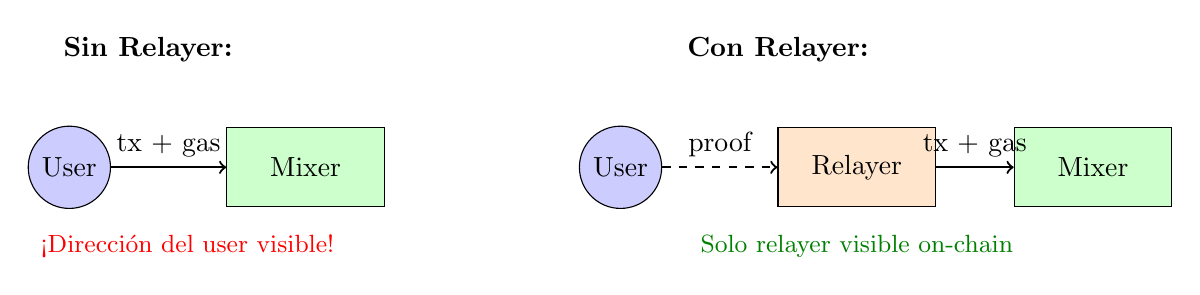
\begin{tikzpicture}[
    user/.style={draw, circle, minimum size=1cm, fill=blue!20},
    contract/.style={draw, rectangle, minimum width=2cm, minimum height=1cm, fill=green!20},
    relayer/.style={draw, rectangle, minimum width=2cm, minimum height=1cm, fill=orange!20},
    arrow/.style={->, thick}
]
    % Sin relayer
    \node at (-4, 3) {\textbf{Sin Relayer:}};
    \node[user] (user1) at (-5, 1.5) {User};
    \node[contract] (contract1) at (-2, 1.5) {Mixer};
    \draw[arrow] (user1) -- node[above] {tx + gas} (contract1);
    \node[red] at (-3.5, 0.5) {\small !`Direcci\'on del user visible!};
    
    % Con relayer
    \node at (4, 3) {\textbf{Con Relayer:}};
    \node[user] (user2) at (2, 1.5) {User};
    \node[relayer] (relay) at (5, 1.5) {Relayer};
    \node[contract] (contract2) at (8, 1.5) {Mixer};
    \draw[arrow, dashed] (user2) -- node[above] {proof} (relay);
    \draw[arrow] (relay) -- node[above] {tx + gas} (contract2);
    \node[green!50!black] at (5, 0.5) {\small Solo relayer visible on-chain};
\end{tikzpicture}
\end{center}

%-------------------------------------------
\subsection{Modelo Econ\'omico}

\begin{itemize}
    \item Fee t\'ipico: 0.1--1\% del retiro
    \item Competencia entre relayers reduce fees
    \item Puede ser centralizado o red descentralizada
    \item Incentivos para uptime y servicio
\end{itemize}

\begin{mathnote}
\textbf{Econom\'ia de relayers:}

\textbf{Ingresos del relayer:}
\begin{itemize}
    \item Fee por transacci\'on: $f$ (ej: 0.3\%)
    \item Volumen diario: $V$ (ej: 1000 ETH)
    \item Ingresos diarios: $f \times V = 3$ ETH
\end{itemize}

\textbf{Costos del relayer:}
\begin{itemize}
    \item Gas por tx: $\sim$0.01 ETH
    \item Infraestructura: servidores, monitoreo
    \item Capital: ETH para pagar gas antes de recibir fee
\end{itemize}

\textbf{Competencia:}
\begin{itemize}
    \item M\'ultiples relayers compiten por transacciones
    \item Usuarios eligen por fee m\'as bajo
    \item Equilibrio de mercado determina fee
\end{itemize}

\textbf{Modelos de implementaci\'on:}
\begin{itemize}
    \item \textbf{Centralizado:} Un operador, riesgo de censura
    \item \textbf{Red P2P:} M\'ultiples operadores, m\'as resistente
    \item \textbf{DAO-managed:} Gobernanza comunitaria
\end{itemize}
\end{mathnote}

%-------------------------------------------
\subsection{Implementaci\'on T\'ecnica}

\begin{example}[Flujo de relayer]
\begin{lstlisting}[style=python]
# 1. Usuario genera prueba localmente
proof = generate_proof(secret, nullifier, merkle_path, recipient)

# 2. Usuario prepara request para relayer
request = {
    ''proof'': proof,
    ''public_inputs'': {
        ''root'': current_merkle_root,
        ''nullifier_hash'': hash(nullifier),
        ''recipient'': recipient_address,
        ''relayer'': relayer_address,
        ''fee'': 0.003 * amount,  # 0.3%
    },
    ''signature'': sign(request, user_key)  # Opcional
}

# 3. Enviar a relayer (off-chain, puede ser HTTPS o Tor)
response = await relayer.submit(request)

# 4. Relayer verifica y envia tx
# En el backend del relayer:
def handle_request(request):
    # Verificar que la prueba es valida
    if not verify_proof(request.proof, request.public_inputs):
        return error(''Invalid proof'')
    
    # Verificar que el fee es suficiente
    if request.fee < min_fee:
        return error(''Fee too low'')
    
    # Enviar tx on-chain
    tx = mixer_contract.withdraw(
        request.proof,
        request.public_inputs
    )
    
    # Relayer paga gas, recibe fee del contrato
    return tx.hash
\end{lstlisting}
\end{example}

%===========================================
\section{Mixers: Tornado Cash, C\'omo Funcionan}
%===========================================

\begin{definition}[Mixer]
Protocolo que mezcla fondos de m\'ultiples usuarios para romper trazabilidad.
\end{definition}

%-------------------------------------------
\subsection{Historia y Contexto}

\begin{remark}
\textbf{Evoluci\'on de los mixers:}

\begin{center}
\begin{tabular}{lll}
\toprule
\textbf{Era} & \textbf{Tecnolog\'ia} & \textbf{Problemas} \\
\midrule
2013 & Mixers centralizados & Confianza en operador \\
2014 & CoinJoin (Bitcoin) & Coordinaci\'on, trazabilidad parcial \\
2016 & Zcash (shielded) & Nueva blockchain requerida \\
2019 & Tornado Cash & ZK en Ethereum, trustless \\
2022 & Tornado sanctioned & Regulaci\'on, debates legales \\
2023+ & Privacy pools & Compliance + privacidad \\
\bottomrule
\end{tabular}
\end{center}
\end{remark}

%-------------------------------------------
\subsection{Arquitectura Tornado Cash}

\begin{enumerate}
    \item \textbf{Deposit:}
    \begin{itemize}
        \item Usuario genera secretos $(s, n)$ localmente
        \item Calcula commitment $C = H(s \| n)$
        \item Env\'ia tx: deposit(C, monto)
        \item Contrato inserta $C$ en Merkle tree
    \end{itemize}
    
    \item \textbf{Wait:}
    \begin{itemize}
        \item M\'as dep\'ositos aumentan anonymity set
        \item Usuario guarda $(s, n)$ de forma segura
    \end{itemize}
    
    \item \textbf{Withdraw:}
    \begin{itemize}
        \item Obtener Merkle proof para $C$
        \item Calcular nullifier $N = H(s)$ (nota: diferente de commitment)
        \item Generar prueba ZK
        \item Enviar v\'ia relayer
        \item Contrato verifica y paga
    \end{itemize}
\end{enumerate}

\begin{center}
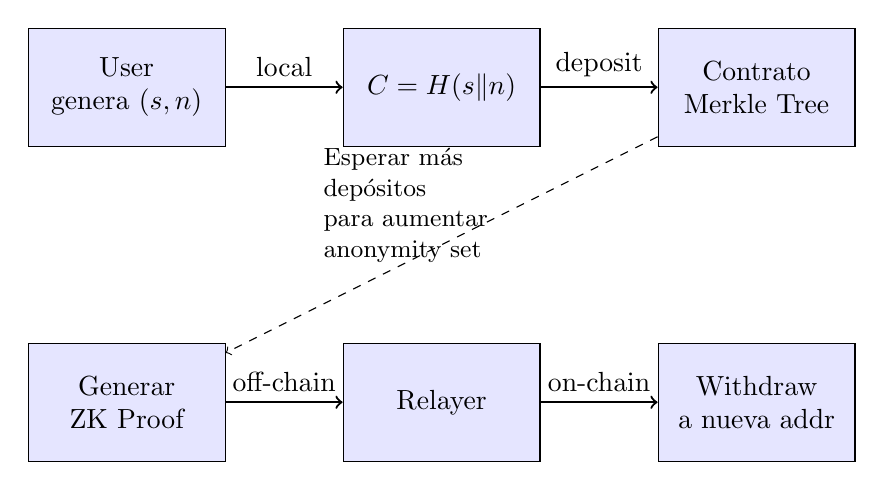
\begin{tikzpicture}[
    box/.style={draw, rectangle, minimum width=2.5cm, minimum height=1.5cm, align=center, fill=blue!10},
    arrow/.style={->, thick},
    note/.style={font=\small, text width=3cm}
]
    % Deposit phase
    \node[box] (user1) at (0, 4) {User\\genera $(s, n)$};
    \node[box] (commit) at (4, 4) {$C = H(s \| n)$};
    \node[box] (contract) at (8, 4) {Contrato\\Merkle Tree};
    
    \draw[arrow] (user1) -- node[above] {local} (commit);
    \draw[arrow] (commit) -- node[above] {deposit} (contract);
    
    % Wait phase
    \node[note] at (4, 2.5) {Esperar m\'as dep\'ositos\\para aumentar\\anonymity set};
    
    % Withdraw phase
    \node[box] (proof) at (0, 0) {Generar\\ZK Proof};
    \node[box] (relayer) at (4, 0) {Relayer};
    \node[box] (withdraw) at (8, 0) {Withdraw\\a nueva addr};
    
    \draw[arrow] (proof) -- node[above] {off-chain} (relayer);
    \draw[arrow] (relayer) -- node[above] {on-chain} (withdraw);
    
    % Connection
    \draw[dashed, ->] (contract) -- (proof);
\end{tikzpicture}
\end{center}

%-------------------------------------------
\subsection{Componentes T\'ecnicos}

\begin{itemize}
    \item Smart contracts (Ethereum)
    \item Circuitos Circom
    \item Frontend (descentralizado v\'ia IPFS)
    \item Red de relayers
    \item Denominaciones fijas: 0.1, 1, 10, 100 ETH
\end{itemize}

\begin{example}[Circuito Tornado Cash (simplificado)]
\begin{lstlisting}[style=circom]
// withdraw.circom (simplificado)
template Withdraw(levels) {
    // Public inputs
    signal input root;
    signal input nullifierHash;
    signal input recipient;
    signal input relayer;
    signal input fee;
    
    // Private inputs (witness)
    signal input secret;
    signal input nullifier;
    signal input pathElements[levels];
    signal input pathIndices[levels];
    
    // 1. Verificar que el commitment esta en el tree
    component hasher = Poseidon(2);
    hasher.inputs[0] <== secret;
    hasher.inputs[1] <== nullifier;
    signal commitment <== hasher.out;
    
    component merkle = MerkleTreeChecker(levels);
    merkle.leaf <== commitment;
    merkle.root <== root;
    for (var i = 0; i < levels; i++) {
        merkle.pathElements[i] <== pathElements[i];
        merkle.pathIndices[i] <== pathIndices[i];
    }
    
    // 2. Verificar nullifier hash
    component nullifierHasher = Poseidon(1);
    nullifierHasher.inputs[0] <== nullifier;
    nullifierHasher.out === nullifierHash;
    
    // 3. Hashear recipient/relayer/fee (anti-frontrun)
    signal recipientSquare;
    recipientSquare <== recipient * recipient;
}
\end{lstlisting}
\end{example}

%===========================================
\section{Nullifiers}
%===========================================

\begin{definition}[Nullifier]
Valor \'unico derivado de un dep\'osito que previene doble gasto.
\end{definition}

Propiedades:
\begin{itemize}
    \item Determin\'istico: mismo dep\'osito $\to$ mismo nullifier
    \item \'Unico: diferentes dep\'ositos $\to$ diferentes nullifiers
    \item No vinculable: observador no puede vincular $N$ con $C$
\end{itemize}

Implementaci\'on t\'ipica:
\[
N = H(\text{secret} \| \text{leaf\_index})
\]

%-------------------------------------------
\subsection{Por qu\'e Necesitamos Nullifiers}

\begin{intuicion}
\textbf{El problema del doble gasto en mixers:}

Sin nullifiers:
\begin{itemize}
    \item Usuario deposita 1 ETH, obtiene commitment $C$
    \item Retira 1 ETH con prueba de que $C$ est\'a en el tree
    \item !`Retira OTRA VEZ con la misma prueba!
    \item El commitment sigue en el tree
    \item Puede retirar infinitamente
\end{itemize}

\textbf{Soluci\'on con nullifiers:}
\begin{itemize}
    \item Al retirar, revela $N = H(\text{secret})$
    \item Contrato registra $N$ en un conjunto de ``usados''
    \item Si $N$ ya est\'a en el conjunto, rechaza
    \item Cada dep\'osito solo puede retirarse una vez
\end{itemize}

\textbf{Propiedad clave:}
\begin{itemize}
    \item $N$ est\'a determinado por el secreto
    \item Pero observador no puede vincular $N$ con $C$
    \item Porque $C = H(\text{secret}, \text{nullifier\_seed})$
    \item Y $N = H(\text{nullifier\_seed})$ usa input diferente
\end{itemize}
\end{intuicion}

\begin{mathnote}
\textbf{Dise\~no criptogr\'afico de nullifiers:}

\textbf{Requerimientos:}
\begin{enumerate}
    \item \textbf{Unicidad:} Diferentes dep\'ositos $\to$ diferentes $N$
    \item \textbf{Determinismo:} Mismo dep\'osito siempre produce mismo $N$
    \item \textbf{No-vinculabilidad:} Dado $N$, no se puede determinar $C$
    \item \textbf{Prueba de conocimiento:} Solo el due\~no puede producir $N$ v\'alido
\end{enumerate}

\textbf{Construcci\'on de Tornado Cash:}
\begin{lstlisting}[style=python]
# Deposit:
secret = random(31)  # bytes
nullifier_seed = random(31)  # bytes

commitment = Poseidon(secret, nullifier_seed)
note = (secret, nullifier_seed, leaf_index)

# Withdraw:
nullifier_hash = Poseidon(nullifier_seed)

# ZK proof demuestra:
# 1. Conoce (secret, nullifier_seed) tal que
#    Poseidon(secret, nullifier_seed) esta en el Merkle tree
# 2. nullifier_hash = Poseidon(nullifier_seed)
\end{lstlisting}

\textbf{Por qu\'e funciona:}
\begin{itemize}
    \item $C$ depende de ambos: secret Y nullifier\_seed
    \item $N$ solo depende de nullifier\_seed
    \item Dado $N$, no puedes deducir secret
    \item Dado $N$, no puedes calcular $C$ sin secret
    \item $\to$ No vinculable
\end{itemize}
\end{mathnote}

%===========================================
\section{Anonymity Set}
%===========================================

\begin{definition}[Anonymity Set]
Conjunto de participantes entre los cuales un usuario es indistinguible.
\end{definition}

\begin{mathnote}
Con $n$ dep\'ositos del mismo monto:
\begin{itemize}
    \item Probabilidad de linking correcto: $1/n$
    \item $n = 100 \to 1\%$
    \item $n = 10,000 \to 0.01\%$
    \item $n = 1,000,000 \to 0.0001\%$
\end{itemize}
\end{mathnote}

%-------------------------------------------
\subsection{Factores que Afectan el Anonymity Set}

Factores que reducen anonymity set:
\begin{itemize}
    \item Depositar y retirar inmediatamente
    \item Montos \'unicos
    \item Misma direcci\'on para deposit y withdraw
    \item Patrones de comportamiento
\end{itemize}

\begin{example}[Ataques al anonymity set]
\textbf{1. Timing attack:}
\begin{lstlisting}[style=python]
# Depositos en pool de 1 ETH:
#     09:00 - Alice deposita
#     09:01 - Bob deposita
#     09:02 - Carol deposita
#     09:03 - Retiro a direccion X
    
# Si hay pocos depositos, probabilidad alta de vincular.
# Con solo 3 depositos: 33% de adivinar.
\end{lstlisting}

\textbf{2. Amount correlation:}
\begin{lstlisting}[style=python]
# Si Alice deposita exactamente 1.337 ETH:
#     Solo ella deposito ese monto
#     Cualquier retiro de 1.337 ETH es de Alice
#     Anonymity set = 1

# Solucion: denominaciones fijas (0.1, 1, 10, 100 ETH)
\end{lstlisting}

\textbf{3. Behavioral patterns:}
\begin{lstlisting}[style=python]
# Alice siempre retira a la misma hora
# Alice siempre usa el mismo relayer
# Alice retira a direcciones que luego interactuan entre si

# Analisis de grafos puede reducir anonymity set
\end{lstlisting}

\textbf{4. Dust attacks:}
\begin{lstlisting}[style=python]
# Atacante envia pequenas cantidades a muchas direcciones
# Rastreo: ''este retiro envio dust a direccion conocida''
# Puede vincular deposito con retiro
\end{lstlisting}
\end{example}

%-------------------------------------------
\subsection{Mejorando el Anonymity Set}

\begin{keyidea}
\textbf{Mejores pr\'acticas para m\'axima privacidad:}

\textbf{1. Esperar tiempo suficiente:}
\begin{itemize}
    \item M\'as tiempo = m\'as dep\'ositos = mayor anonymity set
    \item M\'inimo recomendado: semanas a meses
    \item Ideal: esperar hasta que anonymity set sea grande
\end{itemize}

\textbf{2. Usar denominaciones populares:}
\begin{itemize}
    \item Pools m\'as grandes tienen m\'as usuarios
    \item 0.1 ETH: millones de dep\'ositos
    \item 100 ETH: miles de dep\'ositos
\end{itemize}

\textbf{3. Evitar patrones:}
\begin{itemize}
    \item Variar tiempos de retiro
    \item Usar diferentes relayers
    \item No consolidar retiros
\end{itemize}

\textbf{4. Nueva direcci\'on para cada retiro:}
\begin{itemize}
    \item Nunca reutilizar direcciones de retiro
    \item No enviar desde retiro a direcciones conocidas tuyas
\end{itemize}

\textbf{5. M\'ultiples hops:}
\begin{itemize}
    \item Depositar, retirar, depositar otra vez
    \item Aumenta costo pero mejora privacidad
\end{itemize}
\end{keyidea}

%===========================================
\section{Deposit/Withdraw Flow}
%===========================================

\subsection{Deposit Flow Detallado}

\begin{enumerate}
    \item Usuario genera aleatoriamente:
    \begin{itemize}
        \item $s$: secret (31 bytes)
        \item $n$: nullifier seed (31 bytes)
    \end{itemize}
    \item Calcula $C = \text{Poseidon}(s, n)$
    \item Firma y env\'ia tx con $C$ y monto
    \item Contrato verifica monto y a\~nade $C$ al tree
    \item Usuario almacena ``note'': $(s, n, \text{leafIndex})$
\end{enumerate}

\begin{example}[C\'odigo de dep\'osito]
\begin{lstlisting}[style=python]
# Frontend (JavaScript/Python)
async def deposit(amount):
    # 1. Generar secretos localmente
    secret = crypto.randomBytes(31)
    nullifier_seed = crypto.randomBytes(31)
    
    # 2. Calcular commitment
    commitment = poseidon([secret, nullifier_seed])
    
    # 3. Enviar transaccion
    tx = await tornado_contract.deposit(
        commitment,
        value=amount
    )
    await tx.wait()
    
    # 4. Guardar note (CRITICO! Sin esto, fondos perdidos)
    leaf_index = await get_leaf_index(commitment)
    note = encode_note({
        ''secret'': secret,
        ''nullifier_seed'': nullifier_seed,
        ''leaf_index'': leaf_index,
        ''amount'': amount,
        ''currency'': ''ETH''
    })
    
    # 5. Mostrar note al usuario para backup
    print(f''Your note: {note}'')
    # Formato: tornado-eth-1-0x1234...
    
    return {''tx'': tx, ''note'': note}
\end{lstlisting}
\end{example}

%-------------------------------------------
\subsection{Withdraw Flow Detallado}

\begin{enumerate}
    \item Usuario recupera note $(s, n, \text{idx})$
    \item Obtiene Merkle path para leaf $\text{idx}$
    \item Calcula nullifier $N = \text{Poseidon}(n)$
    \item Genera ZK proof que demuestra:
    \begin{itemize}
        \item Conoce $(s, n)$ tal que $\text{Poseidon}(s, n)$ est\'a en tree
        \item Merkle path es v\'alido para root $R$
        \item $N$ es el nullifier correcto
        \item Recipient address est\'a hasheado en la prueba
    \end{itemize}
    \item Env\'ia $(N, \text{proof}, \text{recipient})$ a relayer
    \item Relayer env\'ia tx al contrato
    \item Contrato verifica:
    \begin{itemize}
        \item $N$ no usado antes
        \item Proof v\'alida
        \item Root $R$ es o fue v\'alido
    \end{itemize}
    \item Contrato registra $N$ y env\'ia fondos
\end{enumerate}

\begin{example}[C\'odigo de retiro]
\begin{lstlisting}[style=python]
# Frontend (JavaScript/Python)
async def withdraw(note_string, recipient_address, relayer_url):
    # 1. Decodificar note
    note = decode_note(note_string)
    secret = note[''secret'']
    nullifier_seed = note[''nullifier_seed'']
    leaf_index = note[''leaf_index'']
    amount = note[''amount'']
    
    # 2. Obtener datos actuales del contrato
    root = await tornado_contract.getLastRoot()
    merkle_proof = await get_merkle_proof(leaf_index)
    
    # 3. Calcular nullifier hash
    nullifier_hash = poseidon([nullifier_seed])
    
    # 4. Generar prueba ZK (costoso, segundos)
    input_data = {
        # Public
        ''root'': root,
        ''nullifierHash'': nullifier_hash,
        ''recipient'': recipient_address,
        ''relayer'': relayer_address,
        ''fee'': relayer_fee,
        
        # Private (witness)
        ''secret'': secret,
        ''nullifier'': nullifier_seed,
        ''pathElements'': merkle_proof.path_elements,
        ''pathIndices'': merkle_proof.path_indices
    }
    
    proof, public_signals = await snarkjs.groth16.fullProve(
        input_data,
        ''withdraw.wasm'',
        ''withdraw.zkey''
    )
    
    # 5. Enviar a relayer
    response = await fetch(relayer_url + ''/relay'', {
        ''method'': ''POST'',
        ''body'': json.dumps({
            ''proof'': proof,
            ''args'': public_signals
        })
    })
    
    # 6. Esperar confirmacion
    tx_hash = (await response.json())[''txHash'']
    return await provider.waitForTransaction(tx_hash)
\end{lstlisting}
\end{example}

%===========================================
\section{Compliance y Proof-of-Innocence}
%===========================================

\begin{definition}[Proof-of-Innocence]
Prueba de que fondos no provienen de fuentes il\'icitas, sin revelar origen exacto.
\end{definition}

Mecanismos:
\begin{itemize}
    \item Probar dep\'osito antes de fecha X (antes de hack)
    \item Probar no-inclusi\'on en lista de direcciones sancionadas
    \item Probar que origen est\'a en ``association set'' leg\'itimo
    \item Viewing keys para auditor\'ia selectiva
\end{itemize}

\begin{keyidea}
\textbf{Privacy Pools (propuesta 2023):}

Respuesta al problema: ``?`C\'omo tener privacidad Y cumplir regulaciones?''

\textbf{Idea:} Association Sets

\begin{lstlisting}[style=python]
# Association Set = conjunto de depositos ''buenos''
#     - Depositantes verificados
#     - Antes de eventos ilicitos conocidos
#     - Aprobados por DAO/comunidad

# Al retirar, pruebo (en ZK):
#     1. Mi deposito esta en el Merkle tree del mixer (privacidad)
#     2. Mi deposito esta en el Association Set (compliance)

# No revelo CUAL deposito, solo que:
#     - Es valido (tengo derecho a retirar)
#     - Es ''inocente'' (pertenece al set bueno)
\end{lstlisting}

\textbf{Beneficios:}
\begin{itemize}
    \item Privacidad: nadie sabe cu\'al dep\'osito espec\'ifico
    \item Compliance: reguladores saben que no es fondos il\'icitos
    \item Flexible: diferentes association sets para diferentes requisitos
\end{itemize}
\end{keyidea}

\begin{bancozk}
\textbf{Compliance en Banco ZK:}

\textbf{Enfoque multi-nivel:}

\textbf{1. Screening de dep\'ositos:}
\begin{itemize}
    \item Verificar que direcci\'on de origen no est\'a sancionada
    \item Opcional: KYC para dep\'ositos grandes
    \item Rechazar dep\'ositos de addresses conocidas como il\'icitas
\end{itemize}

\textbf{2. Proof-of-Innocence al retirar:}
\begin{itemize}
    \item Usuarios pueden generar prueba de association set
    \item Exchanges/servicios pueden requerir esta prueba
    \item Sin revelar dep\'osito espec\'ifico
\end{itemize}

\textbf{3. Viewing keys opcionales:}
\begin{itemize}
    \item Usuario puede revelar historial a auditor espec\'ifico
    \item \'Util para impuestos, compliance corporativo
    \item Solo con consentimiento del usuario
\end{itemize}

\textbf{Arquitectura:}
\begin{lstlisting}[style=python]
# Modo default: privacidad total
#     -> Anonymity set completo
    
# Modo compliance: privacidad + proof-of-innocence
#     -> Prueba de association set
    
# Modo audit: revelacion selectiva
#     -> Viewing key a auditor especifico
\end{lstlisting}
\end{bancozk}

%===========================================
\section{zkEVM}
%===========================================

\begin{definition}[zkEVM]
EVM completa ejecutada dentro de un circuito ZK.
\end{definition}

%-------------------------------------------
\subsection{El Desaf\'io de zkEVM}

\begin{intuicion}
\textbf{?`Por qu\'e es dif\'icil hacer zkEVM?}

La EVM fue dise\~nada para ejecuci\'on, NO para ZK proofs:
\begin{itemize}
    \item \textbf{Keccak256:} Hash usado en todo, pero muy costoso en ZK
    \item \textbf{256 bits:} Aritm\'etica en campo ``inc\'omodo'' para ZK
    \item \textbf{Stack machine:} Acceso din\'amico es caro en circuitos
    \item \textbf{Memoria din\'amica:} Tama\~no variable, dif\'icil de circuitizar
    \item \textbf{Storage:} Merkle Patricia Trie con Keccak (doble problema)
\end{itemize}

\textbf{Trade-off fundamental:}
\begin{itemize}
    \item M\'as compatible con Ethereum $\to$ Circuitos m\'as grandes $\to$ Proofs m\'as lentos
    \item Menos compatible $\to$ Circuitos m\'as eficientes $\to$ Proofs m\'as r\'apidos
\end{itemize}
\end{intuicion}

%-------------------------------------------
\subsection{Tipos de zkEVM}

\begin{center}
\begin{tabular}{clp{6cm}}
\toprule
\textbf{Tipo} & \textbf{Nombre} & \textbf{Descripci\'on} \\
\midrule
1 & Ethereum-equivalent & Id\'entico a Ethereum, incluye todo \\
2 & EVM-equivalent & Compatible con EVM, peque\~nas diferencias \\
3 & EVM-compatible & Algunas modificaciones para eficiencia \\
4 & Language-compatible & Lenguaje propio que compila a EVM-like \\
\bottomrule
\end{tabular}
\end{center}

\begin{itemize}
    \item \textbf{Tipo 1:} Scroll, Taiko (m\'as lento, totalmente compatible)
    \item \textbf{Tipo 2:} Polygon zkEVM (muy compatible)
    \item \textbf{Tipo 3:} Scroll (en desarrollo hacia tipo 1)
    \item \textbf{Tipo 4:} zkSync Era, StarkNet (lenguajes propios)
\end{itemize}

\begin{mathnote}
\textbf{Espectro de compatibilidad:}

\begin{center}
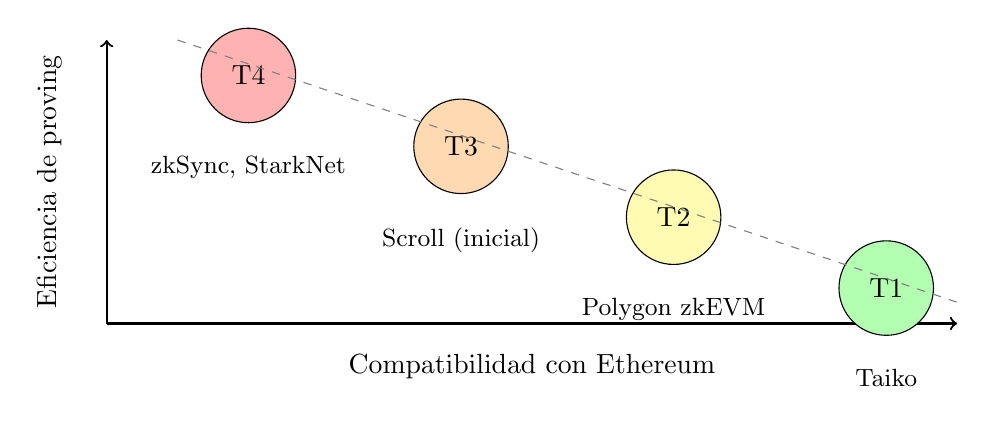
\begin{tikzpicture}[scale=0.9]
    % Eje
    \draw[thick, ->] (0, 0) -- (12, 0);
    \draw[thick, ->] (0, 0) -- (0, 4);
    
    % Labels
    \node[below] at (6, -0.3) {Compatibilidad con Ethereum};
    \node[rotate=90, above] at (-0.5, 2) {Eficiencia de proving};
    
    % Tipos
    \node[draw, circle, fill=red!30, minimum size=1.2cm] (t4) at (2, 3.5) {T4};
    \node[draw, circle, fill=orange!30, minimum size=1.2cm] (t3) at (5, 2.5) {T3};
    \node[draw, circle, fill=yellow!30, minimum size=1.2cm] (t2) at (8, 1.5) {T2};
    \node[draw, circle, fill=green!30, minimum size=1.2cm] (t1) at (11, 0.5) {T1};
    
    % Proyectos
    \node[below=0.3cm of t4] {\small zkSync, StarkNet};
    \node[below=0.3cm of t3] {\small Scroll (inicial)};
    \node[below=0.3cm of t2] {\small Polygon zkEVM};
    \node[below=0.3cm of t1] {\small Taiko};
    
    % Trade-off line
    \draw[dashed, gray] (1, 4) -- (12, 0.3);
\end{tikzpicture}
\end{center}

\textbf{Tipo 1 (Ethereum-equivalent):}
\begin{itemize}
    \item Puede verificar bloques de Ethereum directamente
    \item Mismo state tree (MPT), mismo hash (Keccak)
    \item Contratos de Ethereum funcionan sin cambios
    \item Proving: muy lento (horas por bloque)
\end{itemize}

\textbf{Tipo 2 (EVM-equivalent):}
\begin{itemize}
    \item Mismo bytecode EVM
    \item Peque\~nas diferencias en precompilados, gas costs
    \item Contratos funcionan casi siempre sin cambios
    \item Proving: m\'as r\'apido (minutos)
\end{itemize}

\textbf{Tipo 3 (EVM-compatible):}
\begin{itemize}
    \item Opcodes modificados para eficiencia ZK
    \item Algunos precompilados diferentes
    \item Mayor\'ia de contratos funcionan
    \item Proving: relativamente r\'apido
\end{itemize}

\textbf{Tipo 4 (Language-compatible):}
\begin{itemize}
    \item Lenguaje nuevo (Cairo, Zinc)
    \item Compila a bytecode optimizado para ZK
    \item Contratos deben reescribirse
    \item Proving: muy r\'apido
\end{itemize}
\end{mathnote}

%-------------------------------------------
\subsection{Arquitectura de un zkEVM}

\begin{example}[Componentes de Polygon zkEVM]
\begin{lstlisting}[style=python]
# Arquitectura de Polygon zkEVM:
#
# +------------------+
# |   Transactions   |
# +--------+---------+
#          |
#          v
# +------------------+
# |    Sequencer     | <- Ordena y ejecuta txs
# +--------+---------+
#          |
#          v
# +------------------+
# |   Executor +     | <- Genera trace de ejecucion
# |   State Manager  |
# +--------+---------+
#          |
#          v
# +------------------+
# |  zkProver        | <- Genera ZK proof del trace
# |  (multiples      |
# |   componentes)   |
# +--------+---------+
#          |
#          v
# +------------------+
# |  Aggregator      | <- Agrega proofs, envia a L1
# +--------+---------+
#          |
#          v
# +------------------+
# |  L1 Contract     | <- Verifica proof, actualiza state
# +------------------+

# Componentes del zkProver:
# - Main SM: Orquesta sub-maquinas
# - Arithmetic SM: Operaciones aritmeticas
# - Binary SM: Operaciones de bits
# - Memory SM: Accesos a memoria
# - Storage SM: Accesos a storage (MPT)
# - Keccak SM: Hash Keccak256
# - Poseidon SM: Hash Poseidon (interno)
# - ROM SM: Bytecode execution
\end{lstlisting}
\end{example}

%-------------------------------------------
\subsection{Comparaci\'on de zkEVMs}

\begin{center}
\begin{tabular}{lcccc}
\toprule
\textbf{Proyecto} & \textbf{Tipo} & \textbf{Proof System} & \textbf{Estado} & \textbf{TPS aprox} \\
\midrule
Scroll & 2 & Halo2 & Mainnet & 20--50 \\
Polygon zkEVM & 2--3 & PLONK + STARK & Mainnet & 30--50 \\
zkSync Era & 4 & PLONK & Mainnet & 100+ \\
StarkNet & 4 & STARK & Mainnet & 50--100 \\
Taiko & 1 & Multi-prover & Mainnet & 10--20 \\
Linea & 2 & Custom & Mainnet & 20--40 \\
\bottomrule
\end{tabular}
\end{center}

\begin{remark}
\textbf{Evoluci\'on de zkEVMs (2024--2025):}

\textbf{Tendencias:}
\begin{itemize}
    \item Todos movi\'endose hacia Tipo 1--2 (m\'axima compatibilidad)
    \item Proving paralelo y distribuido
    \item Hardware acceleration (GPU, FPGA)
    \item Pruebas recursivas para batches m\'as grandes
\end{itemize}

\textbf{Desaf\'ios actuales:}
\begin{itemize}
    \item Proving time sigue siendo alto (minutos a horas)
    \item Costo de proving (\$10--100 por bloque)
    \item Descentralizaci\'on de secuenciadores
    \item Bugs en circuitos complejos
\end{itemize}
\end{remark}

%===========================================
\section{zkVM}
%===========================================

\begin{definition}[zkVM]
M\'aquina virtual de prop\'osito general con ejecuci\'on verificable en ZK.
\end{definition}

%-------------------------------------------
\subsection{zkVM vs zkEVM}

\begin{keyidea}
\textbf{Diferencia conceptual:}

\textbf{zkEVM:}
\begin{itemize}
    \item Emula espec\'ificamente la EVM de Ethereum
    \item Objetivo: compatibilidad con ecosistema Ethereum
    \item Trade-off: eficiencia por compatibilidad
\end{itemize}

\textbf{zkVM:}
\begin{itemize}
    \item M\'aquina virtual de prop\'osito general
    \item Objetivo: probar cualquier programa
    \item T\'ipicamente: arquitectura RISC (RISC-V, MIPS)
    \item Trade-off: flexibilidad por simplicidad de circuito
\end{itemize}

\textbf{?`Cu\'ando usar cada uno?}
\begin{itemize}
    \item zkEVM: cuando necesitas compatibilidad con contratos Ethereum
    \item zkVM: cuando escribes programa desde cero y quieres eficiencia
\end{itemize}
\end{keyidea}

%-------------------------------------------
\subsection{RISC Zero}

\begin{itemize}
    \item Ejecuta RISC-V en ZK
    \item Cualquier programa Rust/C verificable
    \item Guest programs + host interaction
    \item Bonsai: proving service en la nube
\end{itemize}

\begin{mathnote}
\textbf{Arquitectura RISC Zero:}

\textbf{Modelo de ejecuci\'on:}
\begin{lstlisting}[style=python]
# Host (no-ZK)          Guest (dentro de ZK)
# +-----------+         +------------------+
# |           |  input  |                  |
# |   Host    +-------->|  Guest Program   |
# |  Program  |         |   (RISC-V)       |
# |           |<--------+                  |
# +-----------+  output +------------------+
#      |                        |
#      v                        v
#   Normal                  ZK Proof
#   execution               of execution
\end{lstlisting}

\textbf{El guest:}
\begin{itemize}
    \item Programa Rust compilado a RISC-V
    \item Ejecutado dentro del zkVM
    \item Toda la ejecuci\'on genera prueba
\end{itemize}

\textbf{El host:}
\begin{itemize}
    \item Prepara inputs para el guest
    \item Ejecuta el guest en el zkVM
    \item Recibe outputs y proof
\end{itemize}
\end{mathnote}

\begin{example}[Programa RISC Zero]
\begin{lstlisting}[style=rust]
// guest/src/main.rs (ejecutado en zkVM)
#![no_main]
use risc0_zkvm::guest::env;

risc0_zkvm::guest::entry!(main);

fn main() {
    // Leer input del host
    let n: u32 = env::read();
    
    // Computacion que queremos probar
    let result = fibonacci(n);
    
    // Escribir output (sera parte de la prueba)
    env::commit(&result);
}

fn fibonacci(n: u32) -> u64 {
    if n <= 1 { return n as u64; }
    let (mut a, mut b) = (0u64, 1u64);
    for _ in 1..n {
        let temp = a + b;
        a = b;
        b = temp;
    }
    b
}

// host/src/main.rs (ejecutado normalmente)
use risc0_zkvm::{default_prover, ExecutorEnv};
use methods::{FIBONACCI_ELF, FIBONACCI_ID};

fn main() {
    // Preparar input
    let n: u32 = 50;
    
    // Configurar environment
    let env = ExecutorEnv::builder()
        .write(&n)
        .unwrap()
        .build()
        .unwrap();
    
    // Ejecutar y generar prueba
    let prover = default_prover();
    let receipt = prover.prove(env, FIBONACCI_ELF).unwrap();
    
    // Verificar
    receipt.verify(FIBONACCI_ID).unwrap();
    
    // Leer resultado
    let result: u64 = receipt.journal.decode().unwrap();
    println!(''fibonacci({}) = {} (verified!)'', n, result);
}
\end{lstlisting}
\end{example}

%-------------------------------------------
\subsection{SP1}

\begin{itemize}
    \item zkVM de Succinct Labs
    \item Muy r\'apido para recursi\'on
    \item Optimizado para blockchain
    \item Soporta Rust nativo
\end{itemize}

\begin{mathnote}
\textbf{Innovaciones de SP1:}

\textbf{1. Precompilados para cripto:}
\begin{itemize}
    \item SHA256, Keccak256 optimizados
    \item Secp256k1, Ed25519 signatures
    \item BN254 pairings
    \item Mucho m\'as r\'apido que implementaci\'on naive en RISC-V
\end{itemize}

\textbf{2. Recursi\'on eficiente:}
\begin{itemize}
    \item Proofs se pueden verificar dentro de SP1
    \item Permite proof aggregation
    \item Ideal para rollups y bridges
\end{itemize}

\textbf{3. Compatibilidad Rust:}
\begin{itemize}
    \item Compila Rust est\'andar (con restricciones)
    \item Crates de crates.io funcionan
    \item Desarrollo similar a programaci\'on normal
\end{itemize}

\textbf{Performance (2024--2025):}
\begin{itemize}
    \item 10--100x m\'as r\'apido que alternativas para ciertos programas
    \item Proving distribuido para programas grandes
    \item Costo: centavos a d\'olares por proof
\end{itemize}
\end{mathnote}

\begin{example}[Programa SP1]
\begin{lstlisting}[style=rust]
// program/src/main.rs
#![no_main]
sp1_zkvm::entrypoint!(main);

use sha2::{Sha256, Digest};

pub fn main() {
    // Leer input
    let preimage = sp1_zkvm::io::read::<Vec<u8>>();
    
    // Calcular hash (usando precompilado optimizado)
    let mut hasher = Sha256::new();
    hasher.update(&preimage);
    let hash = hasher.finalize();
    
    // Commit al resultado
    sp1_zkvm::io::commit(&hash.to_vec());
}

// script/src/main.rs (host)
use sp1_sdk::{ProverClient, SP1Stdin};

fn main() {
    // Setup
    let client = ProverClient::new();
    let mut stdin = SP1Stdin::new();
    
    // Input
    let preimage = b''hello world''.to_vec();
    stdin.write(&preimage);
    
    // Probar
    let (pk, vk) = client.setup(ELF);
    let proof = client.prove(&pk, stdin).unwrap();
    
    // Verificar
    client.verify(&proof, &vk).unwrap();
    
    // Verificar on-chain (Solidity)
    let solidity_proof = proof.solidity_proof();
}
\end{lstlisting}
\end{example}

%-------------------------------------------
\subsection{Otros zkVMs}

Otros proyectos: Valida, Jolt, Nexus.

\begin{remark}
\textbf{Panorama de zkVMs (2024--2025):}

\begin{center}
\begin{tabular}{lllc}
\toprule
\textbf{Proyecto} & \textbf{ISA} & \textbf{Proof System} & \textbf{Estado} \\
\midrule
RISC Zero & RISC-V & STARK & Producci\'on \\
SP1 & RISC-V & STARK + SNARK & Producci\'on \\
Valida & Propio & STARK & Desarrollo \\
Jolt & RISC-V & Lasso lookups & Desarrollo \\
Nexus & RISC-V & Folding & Desarrollo \\
Powdr & Multi-ISA & STARK & Desarrollo \\
\bottomrule
\end{tabular}
\end{center}

\textbf{Tendencias:}
\begin{itemize}
    \item RISC-V dominando como ISA
    \item STARKs para proving principal
    \item SNARKs (Groth16) para verificaci\'on on-chain
    \item Precompilados para operaciones costosas
\end{itemize}
\end{remark}

%-------------------------------------------
\subsection{Aplicaciones de zkVM}

\begin{example}[Casos de uso de zkVM]
\textbf{1. Bridges verificables:}
\begin{lstlisting}[style=python]
# Probar que bloque de Bitcoin es valido
# (verificar proof-of-work, transacciones, etc.)
bitcoin_block = ...
proof = zkvm.prove(validate_bitcoin_block, bitcoin_block)

# Verificar en Ethereum
ethereum_bridge.submit_block(block_header, proof)
\end{lstlisting}

\textbf{2. ZK Coprocessors:}
\begin{lstlisting}[style=python]
# Ejecutar computo costoso off-chain, verificar on-chain
# Ejemplo: calcular resultado de subasta compleja

bids = fetch_bids_from_chain()
winners, proof = zkvm.prove(calculate_auction_result, bids)

auction_contract.finalize(winners, proof)
# Costo: ~200K gas (verificar proof)
# vs millones de gas ejecutando on-chain
\end{lstlisting}

\textbf{3. Rollups con l\'ogica compleja:}
\begin{lstlisting}[style=python]
# zkVM permite rollups con logica arbitraria
# No limitado a EVM

txs = batch_transactions()
new_state = apply_transactions(current_state, txs)
proof = zkvm.prove(state_transition, (current_state, txs, new_state))

rollup_contract.submit_batch(new_state_root, proof)
\end{lstlisting}

\textbf{4. Verificaci\'on de ML inference:}
\begin{lstlisting}[style=python]
# Probar que un modelo de ML produjo cierto output
model_weights = ...
input_data = ...
output, proof = zkvm.prove(ml_inference, (model_weights, input_data))

# Verificar que output es correcto para el modelo dado
verify(proof, model_hash, input_hash, output)
\end{lstlisting}
\end{example}

\begin{bancozk}
\textbf{zkVM en la arquitectura de Banco ZK:}

\textbf{Rol actual:}

Por ahora usamos circuitos Circom espec\'ificos porque:
\begin{itemize}
    \item Circuitos m\'as peque\~nos y eficientes para nuestro caso
    \item Mejor control sobre constraints exactos
    \item Proving m\'as r\'apido para operaciones espec\'ificas
\end{itemize}

\textbf{Futuro potencial con zkVM:}

\textbf{1. Compliance logic:}
\begin{lstlisting}[style=python]
# Logica de compliance puede ser compleja
# zkVM permite escribirla en Rust normal
def check_compliance(tx):
    # Verificar contra listas de sanciones
    # Aplicar reglas de AML
    # Verificar limites de transaccion
    # Todo verificable en ZK
    pass
\end{lstlisting}

\textbf{2. Bridges con otras chains:}
\begin{lstlisting}[style=python]
# Verificar estado de otras blockchains
# Usar zkVM para validar headers/proofs de otras chains
def verify_external_deposit(chain_proof):
    # Verificar consensus de otra chain
    # Validar transaccion de deposito
    # Retornar resultado verificable
    pass
\end{lstlisting}

\textbf{3. Extensibilidad:}
\begin{lstlisting}[style=python]
# Usuarios avanzados podrian definir logica custom
# Ejecutada en zkVM, verificada por el protocolo
def custom_spending_condition(tx):
    # Logica personalizada
    pass
\end{lstlisting}
\end{bancozk}

%===========================================
\section{Resumen del Cap\'itulo}
%===========================================

\begin{keyidea}
\textbf{Puntos clave de Infraestructura ZK:}

\textbf{1. Relayers:}
\begin{itemize}
    \item Env\'ian txs en nombre del usuario
    \item Esenciales para privacidad (evitan link por gas)
    \item Modelo econ\'omico basado en fees
\end{itemize}

\textbf{2. Mixers:}
\begin{itemize}
    \item Tornado Cash: dep\'osito $\to$ espera $\to$ retiro con ZK proof
    \item Nullifiers previenen doble gasto
    \item Anonymity set crece con m\'as usuarios
\end{itemize}

\textbf{3. zkEVM:}
\begin{itemize}
    \item Tipos 1--4: trade-off compatibilidad vs eficiencia
    \item En producci\'on: Scroll, Polygon, zkSync, StarkNet
    \item Proving sigue siendo costoso (minutos--horas)
\end{itemize}

\textbf{4. zkVM:}
\begin{itemize}
    \item Prop\'osito general (RISC-V t\'ipicamente)
    \item RISC Zero, SP1 en producci\'on
    \item Permite probar cualquier programa Rust/C
    \item Aplicaciones: bridges, coprocessors, ML
\end{itemize}
\end{keyidea}

% ============================================
% FIN DEL CAP\'ITULO 2 (CAP 7 ORIGINAL)
% ============================================

% ============================================
% CAP\'ITULO 3: PRIVACIDAD AVANZADA
% (Cap 8 Original $\to$ Cap 3 Vol 2)
% ============================================
\chapter{Privacidad Avanzada}
\label{ch:privacidad-avanzada}

%===========================================
\section{Ring Signatures}
\label{sec:ring-signatures}
%===========================================

\begin{definition}[Ring Signature]
Firma que prueba que uno de $n$ miembros del ``ring'' firm\'o, sin revelar cu\'al.
\end{definition}

Propiedades:
\begin{itemize}
    \item Anonymity: imposible saber qui\'en firm\'o
    \item Unforgeability: solo miembros pueden firmar
    \item Spontaneous: no requiere setup entre miembros
\end{itemize}

%-------------------------------------------
\subsection{Historia y Contexto}

\begin{remark}
\textbf{Evoluci\'on de Ring Signatures:}

\begin{center}
\begin{tabular}{lll}
\toprule
\textbf{A\~no} & \textbf{Desarrollo} & \textbf{Autores} \\
\midrule
2001 & Ring signatures & Rivest, Shamir, Tauman \\
2004 & Linkable ring signatures & Liu, Wei, Wong \\
2012 & CryptoNote (Monero base) & van Saberhagen \\
2015 & Ring Confidential Transactions & Shen Noether \\
2019 & CLSAG (Monero actual) & Goodell et al. \\
2020 & Triptych & Sarang Noether \\
\bottomrule
\end{tabular}
\end{center}

El nombre ``ring signature'' viene de la estructura circular del algoritmo original, donde las firmas de los miembros se ``encadenan'' en un anillo.
\end{remark}

%-------------------------------------------
\subsection{Intuici\'on}

\begin{intuicion}
\textbf{Analog\'ia: La mesa redonda an\'onima}

Imagina una mesa redonda con 10 personas. Una de ellas escribe un mensaje secreto y lo pasa al siguiente. Cada persona puede:
\begin{itemize}
    \item Ser el autor original (solo 1 persona)
    \item O simplemente pasar el mensaje modific\'andolo un poco
\end{itemize}

Al final, el mensaje vuelve al inicio. Un observador ve que:
\begin{itemize}
    \item El mensaje es ``v\'alido'' (la cadena cierra correctamente)
    \item Alguien en la mesa lo escribi\'o
    \item Pero no puede saber qui\'en fue el autor original
\end{itemize}

\textbf{En t\'erminos criptogr\'aficos:}
\begin{itemize}
    \item Las 10 personas son las claves p\'ublicas del ``ring''
    \item El mensaje es lo que se firma
    \item El autor real usa su clave privada para ``iniciar'' el anillo
    \item Los dem\'as son ``se\~nuelos'' que a\~naden plausibilidad
\end{itemize}
\end{intuicion}

%-------------------------------------------
\subsection{Construcci\'on Matem\'atica}

\begin{mathnote}
\textbf{Ring Signature basada en Schnorr (simplificada):}

\textbf{Setup:}
\begin{itemize}
    \item Ring de $n$ claves p\'ublicas: $P_0, P_1, \ldots, P_{n-1}$
    \item El firmante conoce la clave privada $x_\pi$ tal que $P_\pi = x_\pi G$
    \item Mensaje a firmar: $m$
\end{itemize}

\textbf{Signing (el firmante es el \'indice $\pi$):}

\begin{enumerate}
    \item Elegir $\alpha \xleftarrow{\$} \mathbb{Z}_q$ aleatorio
    \item Para $i \neq \pi$, elegir $c_i, s_i \xleftarrow{\$} \mathbb{Z}_q$ aleatorios
    \item Calcular:
    \[ L_\pi = \alpha G \]
    \[ L_i = s_i G + c_i P_i \quad \text{para } i \neq \pi \]
    
    \item Calcular el challenge global:
    \[ c = H(m \| L_0 \| L_1 \| \ldots \| L_{n-1}) \]
    
    \item Calcular $c_\pi$:
    \[ c_\pi = c - \sum_{i \neq \pi} c_i \mod q \]
    
    \item Calcular $s_\pi$:
    \[ s_\pi = \alpha - c_\pi \cdot x_\pi \mod q \]
    
    \item La firma es: $\sigma = (c, s_0, s_1, \ldots, s_{n-1})$
\end{enumerate}

\textbf{Verification:}

\begin{enumerate}
    \item Para cada $i$, calcular:
    \[ L'_i = s_i G + c_i P_i \]
    donde $c_i$ se deriva de la descomposici\'on de $c$
    
    \item Verificar:
    \[ c \stackrel{?}{=} H(m \| L'_0 \| L'_1 \| \ldots \| L'_{n-1}) \]
\end{enumerate}

\textbf{Por qu\'e funciona:}

Para el firmante real $\pi$:
\[ L_\pi = s_\pi G + c_\pi P_\pi = (\alpha - c_\pi x_\pi) G + c_\pi (x_\pi G) = \alpha G \]

Para los dem\'as: $L_i$ es aleatorio (elegimos $c_i, s_i$ al azar).

La firma ``cierra'' correctamente solo si alguien en el ring conoce una clave privada.
\end{mathnote}

%-------------------------------------------
\subsection{Propiedades de Seguridad}

\begin{keyidea}
\textbf{Propiedades formales:}

\textbf{1. Anonimato (Anonymity):}

Dado un ring $\{P_0, \ldots, P_{n-1}\}$ y una firma v\'alida $\sigma$, la probabilidad de adivinar cu\'al $P_i$ es el firmante real es:
\[ \Pr[\text{adivinar } \pi] = \frac{1}{n} \]

Esto se cumple incluso si el adversario conoce todas las claves privadas excepto una.

\textbf{2. Infalsificabilidad (Unforgeability):}

Un adversario que no conoce ninguna clave privada del ring no puede producir una firma v\'alida, excepto con probabilidad negligible.

\textbf{3. Espontaneidad (Spontaneous):}

El firmante puede crear un ring incluyendo claves p\'ublicas de cualquier persona, sin su conocimiento o cooperaci\'on.

Esta propiedad es crucial: no hay ``setup'' previo entre los miembros del ring.
\end{keyidea}

%-------------------------------------------
\subsection{Tama\~no y Eficiencia}

\begin{remark}
\textbf{Trade-offs de ring signatures:}

\begin{center}
\begin{tabular}{lcc}
\toprule
\textbf{Ring Size} & \textbf{Tama\~no Firma} & \textbf{Anonimato} \\
\midrule
2 & $\sim$200 bytes & 50\% \\
11 (Monero) & $\sim$1.5 KB & 91\% \\
100 & $\sim$6.4 KB & 99\% \\
1000 & $\sim$64 KB & 99.9\% \\
\bottomrule
\end{tabular}
\end{center}

\textbf{Problema:} El tama\~no crece linealmente con el ring size.

\textbf{Soluciones modernas:}
\begin{itemize}
    \item \textbf{CLSAG:} Optimizaci\'on que reduce tama\~no $\sim$25\%
    \item \textbf{Triptych:} Tama\~no logar\'itmico $O(\log n)$
    \item \textbf{Seraphis (futuro Monero):} Mejor eficiencia
\end{itemize}
\end{remark}

%===========================================
\subsection{Linkable Ring Signatures}
%===========================================

\begin{definition}[Linkable Ring Signature]
Ring signature que permite detectar si la misma clave firm\'o dos veces.
\end{definition}

\begin{itemize}
    \item Cada firma incluye ``key image'' $I = x \cdot H_p(P)$
    \item Key image es \'unico por clave privada
    \item Permite detectar doble gasto
    \item Usado en Monero
\end{itemize}

%-------------------------------------------
\subsubsection{Por qu\'e Necesitamos Linkability}

\begin{intuicion}
\textbf{El problema del doble gasto con ring signatures:}

Sin linkability:
\begin{itemize}
    \item Alice tiene una moneda (output) con clave $P_A$
    \item Firma con ring $\{P_A, P_B, P_C\}$ para gastar $\to$ OK
    \item Firma OTRA VEZ con ring $\{P_A, P_D, P_E\}$ $\to$ ?`C\'omo detectar?
    \item Las firmas son v\'alidas y no revelan que $P_A$ es el firmante real
    \item !`Doble gasto!
\end{itemize}

\textbf{Con linkability (key images):}
\begin{itemize}
    \item Cada firma incluye key image $I = x_A \cdot H_p(P_A)$
    \item $I$ es determin\'istico para $x_A$
    \item Si Alice firma dos veces, ambas firmas tienen el mismo $I$
    \item Sistema rechaza la segunda firma
    \item Pero observador no sabe que $I$ corresponde a $P_A$
\end{itemize}
\end{intuicion}

%-------------------------------------------
\subsubsection{Construcci\'on de Key Images}

\begin{mathnote}
\textbf{Key Image en Monero:}

Para clave privada $x$ y clave p\'ublica $P = xG$:

\[ I = x \cdot H_p(P) \]

Donde $H_p$ es un hash-to-point (mapea $P$ a un punto de la curva).

\textbf{Propiedades:}

\textbf{1. Determin\'istico:}

Para la misma clave $(x, P)$, siempre produce el mismo $I$.
\[ I_1 = x \cdot H_p(P) = I_2 \]

\textbf{2. No vinculable:}

Dado $I$, no se puede determinar $P$ sin conocer $x$.
\begin{itemize}
    \item $I = x \cdot H_p(P)$
    \item $H_p(P)$ es un punto ``aleatorio'' desde la perspectiva del observador
    \item Sin $x$, no puede verificar si $I$ corresponde a un $P$ espec\'ifico
\end{itemize}

\textbf{3. \'Unico:}

Diferentes claves producen diferentes key images (con probabilidad abrumadora).
\begin{itemize}
    \item Si $P_1 \neq P_2$, entonces $H_p(P_1) \neq H_p(P_2)$
    \item Por lo tanto $I_1 = x_1 H_p(P_1) \neq x_2 H_p(P_2) = I_2$
\end{itemize}
\end{mathnote}

%-------------------------------------------
\subsubsection{CLSAG (Monero Actual)}

\begin{example}[CLSAG - Concise Linkable Spontaneous Anonymous Group Signatures]
\begin{verbatim}
Estructura de firma CLSAG:

Ring: {P_0, P_1, ..., P_{n-1}}  // Claves p\'ublicas
Commitment: {C_0, C_1, ..., C_{n-1}}  // Pedersen commitments

Firma:
    I        // Key image (32 bytes)
    c_0      // Challenge inicial (32 bytes)
    s_0, s_1, ..., s_{n-1}  // Respuestas (32 bytes cada una)
    D        // Commitment auxiliar (32 bytes)

Tama\~no total: 32 * (n + 3) bytes
Para ring size 11: 32 * 14 = 448 bytes (por input)

Mejora vs MLSAG anterior: ~25% m\'as peque\~no
\end{verbatim}

\textbf{Verificaci\'on:}
\begin{enumerate}
    \item Reconstruir todos los $L_i$ y $R_i$ a partir de $c_0$ y los $s_i$
    \item Verificar que el \'ultimo $c_n$ coincide con $c_0$ (cierra el anillo)
    \item Verificar que $I$ no est\'a en la lista de key images usados
\end{enumerate}
\end{example}

%-------------------------------------------
\subsection{Ring Signatures vs Otras T\'ecnicas}

\begin{center}
\begin{tabular}{lccc}
\toprule
\textbf{Propiedad} & \textbf{Ring Sig} & \textbf{ZK Proof} & \textbf{Mixer} \\
\midrule
Anonimato & Ring size & Anonymity set & Anonymity set \\
Tama\~no & $O(n)$ & $O(1)$ & N/A \\
Setup & Ninguno & Posible trusted & Dep\'osito previo \\
Interactividad & No & No & S\'i (2 txs) \\
Doble gasto & Key images & Nullifiers & Nullifiers \\
\bottomrule
\end{tabular}
\end{center}

\begin{bancozk}
\textbf{Ring Signatures en Banco ZK:}

\textbf{?`Por qu\'e NO usamos ring signatures?}

\begin{itemize}
    \item Tama\~no lineal en ring size (ineficiente para L2)
    \item Preferimos ZK proofs con anonymity set completo
    \item Nullifiers logran lo mismo que key images
\end{itemize}

\textbf{Sin embargo, conceptos relacionados que usamos:}

\begin{itemize}
    \item \textbf{Key images $\to$ Nullifiers:} Mismo concepto, diferente implementaci\'on
    \item \textbf{Anonimato de conjunto:} Nuestro anonymity set es TODO el Merkle tree
    \item \textbf{No-linkability:} Nullifiers no revelan qu\'e commitment gastan
\end{itemize}

\textbf{Comparaci\'on:}
\begin{verbatim}
Monero (Ring Signatures):
    - Ring size: 16 (fijo)
    - Anonimato: 1/16 = 6.25% de probabilidad de link
    - Tama\~no tx: ~2-3 KB

Banco ZK (ZK Proofs):
    - Anonymity set: TODO el tree (millones)
    - Anonimato: 1/n donde n = total de deposits
    - Tama\~no tx: ~200-500 bytes (proof)
\end{verbatim}
\end{bancozk}

%===========================================
\section{Stealth Addresses}
\label{sec:stealth-addresses}
%===========================================

\begin{definition}[Stealth Address]
Direcci\'on de un solo uso generada por el sender para el receiver.
\end{definition}

%-------------------------------------------
\subsection{Motivaci\'on}

\begin{intuicion}
\textbf{El problema de las direcciones reutilizadas:}

En Ethereum normal:
\begin{itemize}
    \item Alice publica su direcci\'on: \texttt{0xAlice...}
    \item Bob le env\'ia 1 ETH
    \item Carol le env\'ia 2 ETH
    \item David le env\'ia 0.5 ETH
\end{itemize}

Cualquiera puede ver:
\begin{itemize}
    \item Todos los pagos a Alice
    \item El balance total de Alice
    \item Potencialmente, qui\'enes le pagan
\end{itemize}

\textbf{Con stealth addresses:}
\begin{itemize}
    \item Cada pago va a una direcci\'on DIFERENTE
    \item Las direcciones no est\'an vinculadas p\'ublicamente
    \item Solo Alice puede identificar cu\'ales son suyas
\end{itemize}
\end{intuicion}

%-------------------------------------------
\subsection{Protocolo DKSAP}

Protocolo:
\begin{enumerate}
    \item Receiver publica meta-address: $(A, B) = (aG, bG)$
    \item Sender genera $r$ aleatorio
    \item Calcula stealth address: $P = H(rA)G + B$
    \item Publica $R = rG$ junto con la tx
    \item Receiver escanea: $P' = H(aR)G + B$
    \item Si $P = P'$, puede gastar con $sk = H(aR) + b$
\end{enumerate}

\begin{mathnote}
\textbf{Matem\'aticas del protocolo DKSAP:}

(Dual-Key Stealth Address Protocol)

\textbf{Setup del Receiver:}
\begin{itemize}
    \item Spending key: $b \xleftarrow{\$} \mathbb{Z}_q$
    \item Viewing key: $a \xleftarrow{\$} \mathbb{Z}_q$
    \item Meta-address p\'ublica: $(A, B) = (aG, bG)$
\end{itemize}

\textbf{Env\'io por el Sender:}
\begin{enumerate}
    \item Generar ef\'imero: $r \xleftarrow{\$} \mathbb{Z}_q$
    \item Shared secret: $s = rA = raG$ (sender calcula)
    \item Stealth address: $P = H(s)G + B$
    \item Ephemeral pubkey: $R = rG$
    \item Enviar fondos a $P$, publicar $R$
\end{enumerate}

\textbf{Escaneo por el Receiver:}
\begin{enumerate}
    \item Para cada tx con ephemeral $R$:
    \item Calcular shared secret: $s' = aR = arG = raG = s$
    \item Calcular stealth: $P' = H(s')G + B$
    \item Si $P' = P$ (direcci\'on en la tx), es para m\'i
\end{enumerate}

\textbf{Gasto por el Receiver:}
\begin{itemize}
    \item Clave privada del stealth: $p = H(s) + b$
    \item Verificaci\'on: $pG = H(s)G + bG = P$ \checkmark
\end{itemize}

\textbf{Por qu\'e funciona:}

\begin{align*}
\text{Sender calcula: } s &= r \cdot A = r \cdot aG \\
\text{Receiver calcula: } s' &= a \cdot R = a \cdot rG = raG = s
\end{align*}

Ambos llegan al mismo shared secret sin revelarlo p\'ublicamente.
\end{mathnote}

\begin{center}
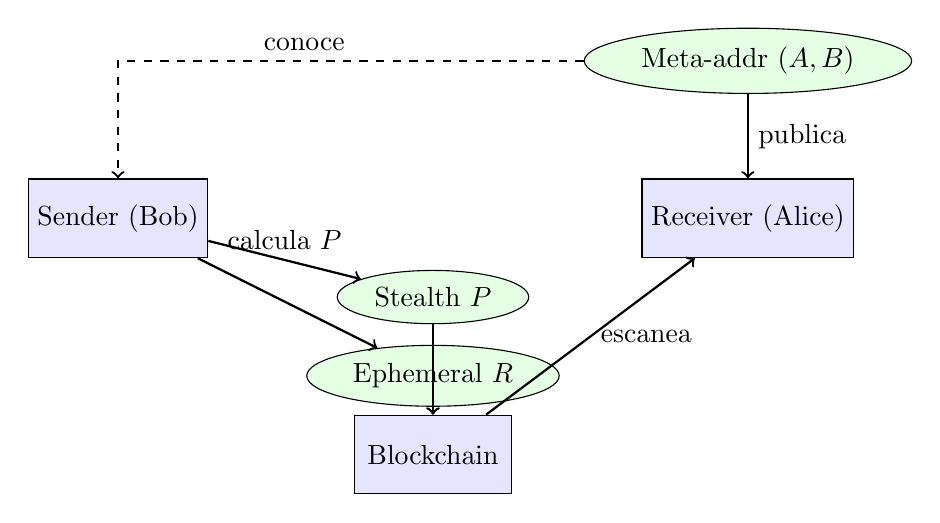
\begin{tikzpicture}[
    actor/.style={draw, rectangle, minimum width=2cm, minimum height=1cm, fill=blue!10},
    key/.style={draw, ellipse, minimum width=1.5cm, fill=green!10},
    arrow/.style={->, thick}
]
    % Actors
    \node[actor] (sender) at (0, 0) {Sender (Bob)};
    \node[actor] (receiver) at (8, 0) {Receiver (Alice)};
    \node[actor] (chain) at (4, -3) {Blockchain};
    
    % Keys
    \node[key] (meta) at (8, 2) {Meta-addr $(A, B)$};
    \node[key] (stealth) at (4, -1) {Stealth $P$};
    \node[key] (ephemeral) at (4, -2) {Ephemeral $R$};
    
    % Arrows
    \draw[arrow] (meta) -- node[right] {publica} (receiver);
    \draw[arrow, dashed] (meta) -| node[above, pos=0.3] {conoce} (sender);
    \draw[arrow] (sender) -- node[above] {calcula $P$} (stealth);
    \draw[arrow] (sender) -- (ephemeral);
    \draw[arrow] (stealth) -- (chain);
    \draw[arrow] (ephemeral) -- (chain);
    \draw[arrow] (chain) -- node[right] {escanea} (receiver);
\end{tikzpicture}
\end{center}

%-------------------------------------------
\subsection{Proyectos e Implementaciones}

\begin{remark}
\textbf{Stealth addresses en la pr\'actica:}

\textbf{Umbra Protocol (Ethereum):}
\begin{itemize}
    \item Implementaci\'on ERC-5564
    \item Registro on-chain de meta-addresses
    \item Soporta ETH y tokens ERC-20
    \item Fee m\'inimo para operaci\'on
\end{itemize}

\textbf{EIP-5564 (Stealth Address Standard):}
\begin{itemize}
    \item Est\'andar propuesto para Ethereum
    \item Define formato de meta-addresses
    \item Interoperabilidad entre wallets
\end{itemize}

\textbf{Desaf\'ios actuales:}
\begin{itemize}
    \item \textbf{Escaneo:} Receiver debe revisar TODAS las txs
    \item \textbf{Gas para gastar:} Stealth address empieza con 0 ETH
    \item \textbf{Compatibilidad:} Wallets deben soportar el est\'andar
\end{itemize}
\end{remark}

%-------------------------------------------
\subsection{Variantes de Stealth Addresses}

\begin{example}[Tipos de stealth addresses]
\textbf{1. Single-key (b\'asico):}
\begin{verbatim}
Meta-address: B = bG (solo spending key)
Stealth: P = H(rB)G + B
Problema: no hay viewing key separada
\end{verbatim}

\textbf{2. Dual-key (DKSAP):}
\begin{verbatim}
Meta-address: (A, B) = (aG, bG)
Stealth: P = H(rA)G + B
Ventaja: viewing key (a) separada de spending key (b)
\end{verbatim}

\textbf{3. Con viewing key delegable:}
\begin{verbatim}
Compartir 'a' con tercero
$\to$ Puede ver todas las txs entrantes
$\to$ No puede gastar (no tiene 'b')
$\to$ \'Util para contadores, auditores
\end{verbatim}
\end{example}

%===========================================
\section{Viewing Keys}
\label{sec:viewing-keys}
%===========================================

\begin{definition}[Viewing Key]
Clave que permite ver transacciones sin poder gastar.
\end{definition}

Usos:
\begin{itemize}
    \item Dar a contador para impuestos
    \item Dar a auditor para compliance
    \item Dar a exchange para verificar dep\'ositos
    \item Spending key siempre privada
\end{itemize}

%-------------------------------------------
\subsection{Tipos de Viewing Keys}

\begin{mathnote}
\textbf{Granularidad de viewing keys:}

\textbf{1. Full Viewing Key:}
\begin{itemize}
    \item Ver TODAS las transacciones (entrantes y salientes)
    \item Conocer balances exactos
    \item Ver destinatarios de pagos salientes
\end{itemize}

\textbf{2. Incoming Viewing Key:}
\begin{itemize}
    \item Ver solo transacciones ENTRANTES
    \item \'Util para exchanges: verificar dep\'ositos
    \item No revela gastos del usuario
\end{itemize}

\textbf{3. Outgoing Viewing Key:}
\begin{itemize}
    \item Ver solo transacciones SALIENTES
    \item Menos com\'un
    \item \'Util para auditor\'ia de gastos
\end{itemize}

\textbf{4. Per-transaction Viewing Key:}
\begin{itemize}
    \item Revelar UNA transacci\'on espec\'ifica
    \item M\'axima granularidad
    \item Probar un pago sin revelar historial
\end{itemize}
\end{mathnote}

%-------------------------------------------
\subsection{Implementaciones}

\begin{example}[Viewing keys en Zcash]
\begin{verbatim}
Jerarqu\'ia de claves en Zcash:

spending_key (sk)
    |
    |---- ask (spend authorizing key)
    |   \---- ak = ask * G (verificaci\'on de gasto)
    |
    |---- nsk (nullifier private key)
    |   \---- nk = nsk * G (generaci\'on de nullifiers)
    |
    \---- ovk (outgoing viewing key)
        \---- Para ver txs salientes

full_viewing_key (fvk) = (ak, nk, ovk)
    $\to$ Puede ver todas las txs
    $\to$ No puede gastar (no tiene ask)

incoming_viewing_key (ivk) = derivado de (ak, nk)
    $\to$ Solo puede ver txs entrantes
    $\to$ No puede ver salientes ni gastar
\end{verbatim}
\end{example}

%-------------------------------------------
\subsection{Casos de Uso}

\begin{keyidea}
\textbf{Escenarios pr\'acticos:}

\textbf{1. Impuestos:}
\begin{verbatim}
Usuario genera viewing key
    $\to$ Da al contador
    $\to$ Contador puede ver historial para calcular impuestos
    $\to$ Contador NO puede gastar fondos
    $\to$ Usuario mantiene privacidad de spending key
\end{verbatim}

\textbf{2. Compliance empresarial:}
\begin{verbatim}
Empresa tiene wallet corporativo
    $\to$ CFO tiene spending key
    $\to$ Auditor externo recibe viewing key
    $\to$ Auditor verifica flujos sin riesgo de robo
    $\to$ Cumple con regulaciones financieras
\end{verbatim}

\textbf{3. Exchanges (incoming only):}
\begin{verbatim}
Usuario quiere depositar en exchange
    $\to$ Exchange da direcci\'on de dep\'osito
    $\to$ Exchange tiene incoming viewing key
    $\to$ Puede verificar dep\'ositos autom\'aticamente
    $\to$ No puede ver otros gastos del usuario
\end{verbatim}

\textbf{4. Herencia/Recovery:}
\begin{verbatim}
Usuario crea viewing key para familiar
    $\to$ Familiar puede monitorear actividad
    $\to$ Si usuario fallece, familiar sabe qu\'e hay
    $\to$ Spending key guardada en testamento seguro
\end{verbatim}
\end{keyidea}

%-------------------------------------------
\subsection{Viewing Keys vs ZK Disclosure}

\begin{remark}
\textbf{Dos enfoques para revelaci\'on selectiva:}

\textbf{Viewing Keys:}
\begin{itemize}
    \item Revelan TODO (o categor\'ia completa)
    \item Una vez compartida, acceso permanente
    \item M\'as simple de implementar
    \item Requiere confiar en el receptor
\end{itemize}

\textbf{ZK Proofs de disclosure:}
\begin{itemize}
    \item Revelan EXACTAMENTE lo necesario
    \item Por transacci\'on o afirmaci\'on
    \item M\'as complejo pero m\'as preciso
    \item ``Pruebo que pagu\'e, sin revelar cu\'anto''
\end{itemize}

\textbf{Ejemplo comparativo:}
\begin{verbatim}
Escenario: Probar que pagu\'e alquiler de $1000

Con viewing key:
    $\to$ Propietario ve TODAS mis transacciones
    $\to$ Ve mi salario, otros gastos, etc.
    $\to$ Mucha informaci\'on extra revelada

Con ZK proof:
    $\to$ Genero prueba: ''tengo tx de $1000 a address X en fecha Y''
    $\to$ Propietario verifica la prueba
    $\to$ No ve nada m\'as de mi historial
    $\to$ Privacidad preservada
\end{verbatim}
\end{remark}

\begin{bancozk}
\textbf{Viewing Keys en Banco ZK:}

\textbf{Dise\~no de claves:}

\begin{verbatim}
master_key
    |
    |---- spending_key
    |   $\to$ Autoriza transacciones
    |   $\to$ NUNCA se comparte
    |
    |---- full_viewing_key
    |   $\to$ Ver todas las transacciones
    |   $\to$ Para auditor\'ia completa
    |
    |---- incoming_viewing_key  
    |   $\to$ Solo dep\'ositos entrantes
    |   $\to$ Para exchanges/servicios
    |
    \---- proof_generation_key
        $\to$ Generar ZK proofs
        $\to$ Sin capacidad de gasto
\end{verbatim}

\textbf{Casos de uso soportados:}

\begin{itemize}
    \item \textbf{Compliance:} Usuario puede probar origen de fondos a regulador
    \item \textbf{Impuestos:} Exportar historial para declaraci\'on
    \item \textbf{Auditor\'ia:} Empresas pueden dar viewing keys a auditores
    \item \textbf{Recuperaci\'on:} Viewing key en backup, spending key en hardware wallet
\end{itemize}

\textbf{Implementaci\'on t\'ecnica:}
\begin{verbatim}
// Derivaci\'on de viewing keys
spending_key = random()
viewing_key = derive_viewing(spending_key)

// Escaneo de transacciones
for commitment in merkle_tree:
    if can_decrypt(commitment, viewing_key):
        // Es m\'ia, extraer detalles
        (amount, sender, memo) = decrypt(commitment, viewing_key)

// Generar prueba de propiedad
proof = prove_ownership(commitment, viewing_key)
// Prueba: ''puedo ver este commitment'' sin revelar spending key
\end{verbatim}
\end{bancozk}

%===========================================
\section{Mixnets}
\label{sec:mixnets}
%===========================================

\begin{definition}[Mixnet]
Red de servidores que mezclan mensajes en capas para anonimato.
\end{definition}

%-------------------------------------------
\subsection{Historia y Contexto}

\begin{remark}
\textbf{Evoluci\'on de las redes de anonimato:}

\begin{center}
\begin{tabular}{lll}
\toprule
\textbf{A\~no} & \textbf{Tecnolog\'ia} & \textbf{Innovaci\'on} \\
\midrule
1981 & Mix networks (Chaum) & Concepto original \\
1996 & Onion routing & Capas de encriptaci\'on \\
2002 & Tor & Implementaci\'on pr\'actica \\
2003 & I2P & Red interna an\'onima \\
2018 & Nym & Mixnet con incentivos crypto \\
\bottomrule
\end{tabular}
\end{center}

\textbf{David Chaum} (1981) invent\'o las mix networks como soluci\'on al problema de comunicaci\'on an\'onima. La idea: si muchos mensajes pasan por un ``mezclador'', es dif\'icil correlacionar entrada con salida.
\end{remark}

%-------------------------------------------
\subsection{Arquitectura}

\begin{enumerate}
    \item Mensaje encriptado en m\'ultiples capas
    \item Cada mix node remueve una capa y reordena
    \item Delays aleatorios en cada hop
    \item Cover traffic para resistir timing analysis
\end{enumerate}

\begin{center}
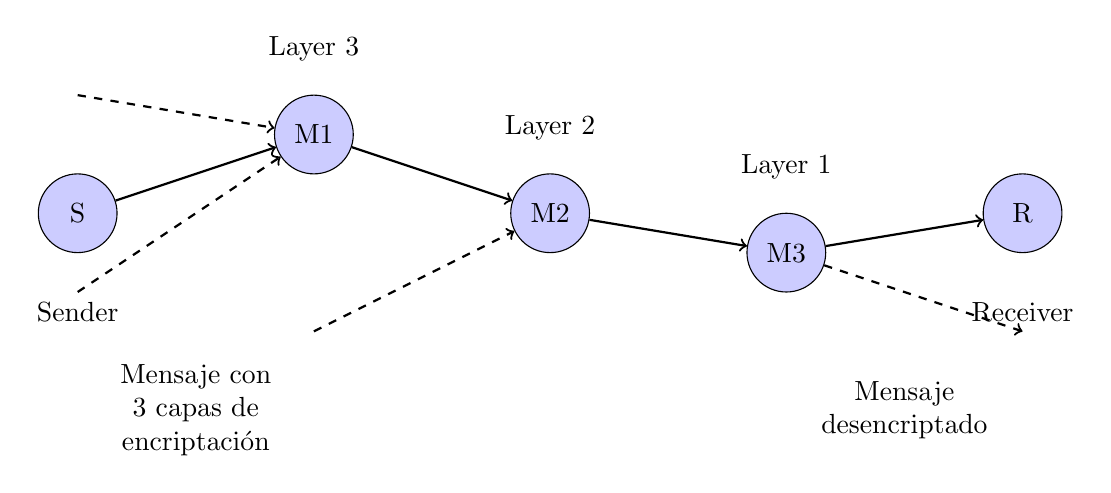
\begin{tikzpicture}[
    node/.style={draw, circle, minimum size=1cm, fill=blue!20},
    msg/.style={draw, rectangle, minimum width=0.5cm, minimum height=0.3cm},
    arrow/.style={->, thick}
]
    % Sender
    \node[node] (sender) at (0, 0) {S};
    
    % Mix nodes
    \node[node] (mix1) at (3, 1) {M1};
    \node[node] (mix2) at (6, 0) {M2};
    \node[node] (mix3) at (9, -0.5) {M3};
    
    % Receiver
    \node[node] (receiver) at (12, 0) {R};
    
    % Messages entering mix1
    \draw[arrow] (sender) -- (mix1);
    \draw[arrow, dashed] (0, 1.5) -- (mix1);
    \draw[arrow, dashed] (0, -1) -- (mix1);
    
    % Messages between mixes
    \draw[arrow] (mix1) -- (mix2);
    \draw[arrow, dashed] (3, -1.5) -- (mix2);
    
    \draw[arrow] (mix2) -- (mix3);
    
    \draw[arrow] (mix3) -- (receiver);
    \draw[arrow, dashed] (mix3) -- (12, -1.5);
    
    % Labels
    \node[below=0.5cm of sender] {Sender};
    \node[below=0.5cm of receiver] {Receiver};
    \node[above=0.3cm of mix1] {Layer 3};
    \node[above=0.3cm of mix2] {Layer 2};
    \node[above=0.3cm of mix3] {Layer 1};
    
    % Encryption layers
    \node[text width=3cm, align=center] at (1.5, -2.5) {Mensaje con\\3 capas de\\encriptaci\'on};
    \node[text width=3cm, align=center] at (10.5, -2.5) {Mensaje\\desencriptado};
\end{tikzpicture}
\end{center}

\begin{mathnote}
\textbf{Encriptaci\'on en capas (Sphinx):}

\textbf{Preparaci\'on del mensaje:}

Para enviar mensaje $m$ a trav\'es de nodos $N_1, N_2, N_3$:

\begin{verbatim}
// Claves p\'ublicas de los mix nodes
pk_1, pk_2, pk_3 = public_keys_of_route

// Generar claves de sesi\'on para cada hop
session_1 = ECDH(ephemeral, pk_1)
session_2 = ECDH(ephemeral, pk_2)
session_3 = ECDH(ephemeral, pk_3)

// Encriptar en capas (de adentro hacia afuera)
layer_3 = Enc(session_3, m || recipient)
layer_2 = Enc(session_2, layer_3 || next_hop_3)
layer_1 = Enc(session_1, layer_2 || next_hop_2)

// Enviar layer_1 al primer nodo
\end{verbatim}

\textbf{Procesamiento en cada nodo:}

\begin{verbatim}
// Nodo N_i recibe paquete encriptado
function process(encrypted_packet):
    // Derivar clave de sesi\'on
    session = ECDH(my_private_key, ephemeral_from_packet)
    
    // Desencriptar una capa
    (inner_layer, next_hop) = Dec(session, encrypted_packet)
    
    // A\~nadir delay aleatorio
    delay(random_milliseconds())
    
    // Reordenar con otros paquetes (batch)
    add_to_batch(inner_layer, next_hop)
    
    // Enviar cuando batch est\'a listo
    send_batch()
\end{verbatim}
\end{mathnote}

%-------------------------------------------
\subsection{Cover Traffic}

\begin{keyidea}
\textbf{?`Por qu\'e cover traffic?}

\textbf{Problema: Timing attacks}

Sin cover traffic:
\begin{itemize}
    \item Adversario observa: mensaje entra a las 10:00:00.000
    \item Observa: mensaje sale a las 10:00:00.150 (150ms delay)
    \item Correlaciona por timing, incluso sin ver contenido
\end{itemize}

\textbf{Soluci\'on: Cover traffic (mensajes dummy)}

Con cover traffic:
\begin{itemize}
    \item Red genera mensajes falsos constantemente
    \item Todos los mensajes lucen iguales (mismo tama\~no)
    \item Adversario no puede distinguir real de dummy
    \item Timing analysis mucho m\'as dif\'icil
\end{itemize}

\textbf{Trade-off:}
\begin{itemize}
    \item M\'as cover traffic $\to$ Mejor privacidad
    \item M\'as cover traffic $\to$ Mayor costo (ancho de banda)
    \item Nym incentiva cover traffic con tokens
\end{itemize}
\end{keyidea}

%-------------------------------------------
\subsection{Nym Network}

\begin{itemize}
    \item Mixnet moderno con incentivos crypto
    \item NYM token para pagar y stakear
    \item Cover traffic autom\'atico
    \item SDK para aplicaciones
    \item Mejor resistencia a timing que Tor
\end{itemize}

\begin{example}[Arquitectura Nym]
\begin{verbatim}
Componentes de Nym:

1. Mix Nodes (3 capas)
   |---- Layer 1: Recibe del cliente
   |---- Layer 2: Intermediario
   \---- Layer 3: Env\'ia al gateway de salida

2. Gateways
   |---- Entry Gateway: Conexi\'on de clientes
   \---- Exit Gateway: Conexi\'on a internet/servicios

3. Validators (Cosmos SDK)
   |---- Consensus sobre estado de la red
   |---- Distribuci\'on de recompensas
   \---- Slashing de nodos maliciosos

4. NYM Token
   |---- Staking en mix nodes
   |---- Pago por uso de la red
   \---- Governance

Flujo de un mensaje:
Client $\to$ Entry Gateway $\to$ Mix L1 $\to$ Mix L2 $\to$ Mix L3 
      $\to$ Exit Gateway $\to$ Destination

Incentivos:
- Mix nodes reciben NYM por procesar tr\'afico
- Cover traffic cuenta para recompensas
- Usuarios pagan por ancho de banda
\end{verbatim}
\end{example}

%-------------------------------------------
\subsection{Mixnets vs Tor}

\begin{center}
\begin{tabular}{lcc}
\toprule
\textbf{Propiedad} & \textbf{Mixnet (Nym)} & \textbf{Tor} \\
\midrule
Latencia & Alta (segundos) & Baja (ms) \\
Resistencia timing & Alta & Media \\
Cover traffic & S\'i & No \\
Modelo de incentivos & Crypto tokens & Voluntarios \\
Decentralizaci\'on & Mayor & Media \\
Uso t\'ipico & Mensajer\'ia & Navegaci\'on \\
\bottomrule
\end{tabular}
\end{center}

%===========================================
\section{Tor e I2P}
\label{sec:tor-i2p}
%===========================================

\subsection{Tor (The Onion Router)}

\begin{itemize}
    \item 3 nodos: guard, middle, exit
    \item Baja latencia (segundos)
    \item Vulnerable a timing attacks
    \item Onion services (.onion)
\end{itemize}

%-------------------------------------------
\subsubsection{Arquitectura de Tor}

\begin{mathnote}
\textbf{C\'omo funciona Tor:}

\textbf{Circuito Tor (3 hops):}
\begin{verbatim}
Usuario $\to$ Guard Node $\to$ Middle Node $\to$ Exit Node $\to$ Destino
           (fijo)       (rotativo)    (rotativo)
\end{verbatim}

\textbf{Guard Node:}
\begin{itemize}
    \item Primer punto de contacto
    \item Se mantiene fijo por meses
    \item Raz\'on: evitar ataques de rotaci\'on de guards
    \item Conoce la IP del usuario
\end{itemize}

\textbf{Middle Node:}
\begin{itemize}
    \item Intermediario
    \item Solo sabe: viene del guard, va al exit
    \item No conoce origen ni destino real
\end{itemize}

\textbf{Exit Node:}
\begin{itemize}
    \item Conexi\'on al destino final
    \item Ve el tr\'afico (si no es HTTPS)
    \item No conoce el origen (usuario)
    \item Punto m\'as ``peligroso'' para operadores
\end{itemize}
\end{mathnote}

%-------------------------------------------
\subsubsection{Onion Services}

\begin{example}[Onion Services (.onion)]
\begin{verbatim}
Servicio tradicional:
    Usuario $\to$ Tor $\to$ Exit Node $\to$ servidor.com
    
    Problema: Exit node ve la conexi\'on al servidor
    Problema: Servidor ve IP del exit node

Onion Service:
    Usuario $\to$ Tor $\to$ Rendezvous Point $\leftarrow$ Tor $\leftarrow$ Servicio .onion
    
    Ventajas:
    - No hay exit node (todo dentro de Tor)
    - Servidor tambi\'en es an\'onimo
    - Comunicaci\'on end-to-end encriptada
    
Direcciones .onion:
    - v2 (deprecated): 16 caracteres
    - v3 (actual): 56 caracteres
\end{verbatim}
\end{example}

%-------------------------------------------
\subsubsection{Integraci\'on con Crypto}

\begin{remark}
\textbf{Usos de Tor en cryptocurrency:}

\textbf{1. Conexi\'on a nodos:}
\begin{verbatim}
# Bitcoin Core con Tor
bitcoind -proxy=127.0.0.1:9050

# Monero con Tor
monerod --tx-proxy tor,127.0.0.1:9050
\end{verbatim}

\textbf{2. Wallets que usan Tor:}
\begin{itemize}
    \item Wasabi Wallet (Bitcoin, Tor por defecto)
    \item Samourai Wallet (Bitcoin, Tor opcional)
    \item Electrum (Tor opcional)
\end{itemize}

\textbf{3. Relayers como onion services:}
\begin{verbatim}
# Tornado Cash ten\'ia relayers en .onion
# Permite submittir proofs sin revelar IP
relayer.onion/submit_proof
\end{verbatim}

\textbf{4. Block explorers:}
\begin{itemize}
    \item Blockchair tiene versi\'on .onion
    \item Mempool.space tiene .onion
    \item Consultar sin revelar qu\'e addresses te interesan
\end{itemize}
\end{remark}

%-------------------------------------------
\subsection{I2P (Invisible Internet Project)}

\begin{itemize}
    \item Garlic routing: m\'ultiples mensajes juntos
    \item Red interna (no exit nodes por defecto)
    \item Mayor latencia
    \item Mejor para servicios dentro de I2P
\end{itemize}

\begin{mathnote}
\textbf{Diferencias clave I2P vs Tor:}

\textbf{Modelo de red:}
\begin{itemize}
    \item Tor: Principalmente para acceder a internet normal
    \item I2P: Dise\~nado como red interna (``darknet'')
\end{itemize}

\textbf{Garlic routing:}
\begin{verbatim}
Tor (Onion): Cada mensaje se encripta individualmente
    Msg1 $\to$ [Enc(Enc(Enc(Msg1)))]
    Msg2 $\to$ [Enc(Enc(Enc(Msg2)))]

I2P (Garlic): M\'ultiples mensajes se encriptan juntos
    Msg1 + Msg2 + Msg3 $\to$ [Enc(Enc(Enc(Msg1, Msg2, Msg3)))]
    
Ventaja: M\'as dif\'icil correlacionar mensajes individuales
\end{verbatim}

\textbf{T\'uneles unidireccionales:}
\begin{verbatim}
Tor: Circuito bidireccional
    A $\leftarrow$$\to$ Guard $\leftarrow$$\to$ Middle $\leftarrow$$\to$ Exit $\leftarrow$$\to$ B

I2P: T\'uneles separados para entrada/salida
    A $\to$ Outbound tunnel $\to$ B
    B $\to$ Outbound tunnel $\to$ A
    
Ventaja: Compromiso de un t\'unel no afecta al otro
\end{verbatim}
\end{mathnote}

\begin{example}[I2P en crypto]
\begin{verbatim}
Monero tiene soporte nativo para I2P:

# Configuraci\'on de Monero con I2P
monerod --tx-proxy i2p,127.0.0.1:4447

Kovri (proyecto relacionado):
- Router I2P en C++ para Monero
- Integraci\'on nativa con el daemon
- Objetivo: Monero completamente sobre I2P

Servicios I2P (.i2p):
- Exploradores de bloques
- Pools de miner\'ia
- Nodos seed
\end{verbatim}
\end{example}

%-------------------------------------------
\subsection{Comparaci\'on de Tecnolog\'ias de Anonimato de Red}

\begin{center}
\begin{tabular}{lcccc}
\toprule
\textbf{Aspecto} & \textbf{Tor} & \textbf{I2P} & \textbf{Nym} & \textbf{VPN} \\
\midrule
Latencia & Baja & Media & Alta & Muy baja \\
Timing resistance & Baja & Media & Alta & Ninguna \\
Decentralizaci\'on & Media & Alta & Alta & Ninguna \\
Exit nodes & S\'i & Opcional & S\'i & S\'i \\
Incentivos & Ninguno & Ninguno & Crypto & Pago \\
Madurez & Alta & Media & Baja & Alta \\
\bottomrule
\end{tabular}
\end{center}

\begin{bancozk}
\textbf{Integraci\'on de red an\'onima en Banco ZK:}

\textbf{Capas de privacidad:}

\begin{verbatim}
Capa de aplicaci\'on: ZK proofs (privacidad de datos)
Capa de red: Tor/Nym (privacidad de IP)

Sin protecci\'on de red:
    $\to$ Observador ve: IP X consult\'o balance de cuenta Y
    $\to$ Aunque balance est\'a encriptado, se filtra metadata

Con protecci\'on de red:
    $\to$ Observador ve: nodo Tor consult\'o algo
    $\to$ No puede vincular IP con cuenta
\end{verbatim}

\textbf{Recomendaciones para usuarios:}

\begin{itemize}
    \item \textbf{M\'inimo:} Usar Tor para consultas de balance
    \item \textbf{Recomendado:} Tor para todas las interacciones
    \item \textbf{Paranoico:} Nym para resistencia a timing
\end{itemize}

\textbf{Infraestructura:}

\begin{itemize}
    \item Relayers disponibles como onion services
    \item Nodos de la red accesibles v\'ia Tor
    \item SDK con soporte para SOCKS5 proxy
\end{itemize}

\textbf{C\'odigo ejemplo:}
\begin{verbatim}
// Configurar cliente con Tor
const client = new BancoZKClient({
    rpcUrl: ''http://localhost:8545'',
    proxy: {
        type: ''socks5'',
        host: ''127.0.0.1'',
        port: 9050  // Tor SOCKS proxy
    }
});

// O usar relayer .onion
const relayer = ''http://bancozk...onion/relay'';
await client.submitViaRelayer(proof, relayer);
\end{verbatim}
\end{bancozk}

%===========================================
\section{MPC (Multi-Party Computation)}
\label{sec:mpc}
%===========================================

\begin{definition}[MPC]
Protocolo donde m\'ultiples partes computan una funci\'on sin revelar sus inputs.
\end{definition}

\[
f(x_1, x_2, \ldots, x_n) \to (y_1, y_2, \ldots, y_n)
\]

Cada parte $i$ conoce solo $x_i$ y aprende solo $y_i$.

%-------------------------------------------
\subsection{Historia y Motivaci\'on}

\begin{remark}
\textbf{Historia de MPC:}

\begin{center}
\begin{tabular}{lll}
\toprule
\textbf{A\~no} & \textbf{Desarrollo} & \textbf{Autores} \\
\midrule
1982 & Millionaires' Problem & Andrew Yao \\
1986 & Garbled Circuits & Yao \\
1987 & BGW Protocol & Ben-Or, Goldwasser, Wigderson \\
1988 & GMW Protocol & Goldreich, Micali, Wigderson \\
2004 & Fairplay (primera impl.) & Malkhi et al. \\
2009 & SPDZ (eficiente) & Damg?rd et al. \\
2017 & MPC en crypto ceremonies & Zcash, Ethereum \\
\bottomrule
\end{tabular}
\end{center}
\end{remark}

\begin{intuicion}
\textbf{El problema de los millonarios (Yao, 1982):}

Alice y Bob quieren saber qui\'en es m\'as rico, sin revelar sus fortunas exactas.

\textbf{Requisitos:}
\begin{itemize}
    \item Alice no revela su fortuna a Bob
    \item Bob no revela su fortuna a Alice
    \item Al final, ambos saben qui\'en tiene m\'as
    \item Ninguno aprende la cantidad del otro
\end{itemize}

\textbf{Sin MPC:}
\begin{itemize}
    \item Opci\'on 1: Confiar en tercero $\to$ Pero ese tercero conoce ambas fortunas
    \item Opci\'on 2: Revelar $\to$ Pierde privacidad
    \item Opci\'on 3: No calcular $\to$ No se obtiene resultado
\end{itemize}

\textbf{Con MPC:}
\begin{itemize}
    \item Alice y Bob ejecutan protocolo entre ellos
    \item Al final: ``Alice tiene m\'as'' o ``Bob tiene m\'as''
    \item Ninguno aprendi\'o el n\'umero del otro
    \item Sin tercero de confianza
\end{itemize}
\end{intuicion}

%-------------------------------------------
\subsection{T\'ecnicas Fundamentales}

\begin{itemize}
    \item \textbf{Garbled Circuits:} Una parte ``garbles'', otra eval\'ua
    \item \textbf{Secret Sharing:} Datos divididos entre partes
    \item \textbf{Oblivious Transfer:} Base de muchos protocolos
\end{itemize}

%-------------------------------------------
\subsubsection{Secret Sharing}

\begin{mathnote}
\textbf{Shamir Secret Sharing (SSS):}

\textbf{Objetivo:} Dividir secreto $s$ entre $n$ partes, requiriendo $t$ para reconstruir.

\textbf{Construcci\'on:}
\begin{enumerate}
    \item Elegir polinomio aleatorio de grado $t-1$:
    \[ p(x) = s + a_1 x + a_2 x^2 + \ldots + a_{t-1} x^{t-1} \]
    donde $p(0) = s$ (el secreto)
    
    \item Dar a cada parte $i$ el punto $(i, p(i))$
    
    \item Con $t$ puntos, se puede interpolar el polinomio (Lagrange)
    
    \item Con menos de $t$ puntos, el secreto es completamente oculto
\end{enumerate}

\textbf{Ejemplo (2-de-3):}
\begin{verbatim}
Secreto: s = 42
Polinomio: p(x) = 42 + 7x  (grado 1, necesita 2 puntos)

Shares:
    Parte 1: (1, p(1)) = (1, 49)
    Parte 2: (2, p(2)) = (2, 56)
    Parte 3: (3, p(3)) = (3, 63)

Reconstrucci\'on con partes 1 y 2:
    Interpolaci\'on de Lagrange:
    p(0) = 49 * (0-2)/(1-2) + 56 * (0-1)/(2-1)
         = 49 * 2 + 56 * (-1)
         = 98 - 56 = 42 $\checkmark$
\end{verbatim}

\textbf{Propiedad aditiva:}

Si $[a]$ y $[b]$ son shares de $a$ y $b$:
\[ [a] + [b] = [a + b] \]

Cada parte puede sumar localmente sus shares, resultado es share de la suma.
\end{mathnote}

%-------------------------------------------
\subsubsection{Garbled Circuits}

\begin{keyidea}
\textbf{Garbled Circuits (Yao):}

\textbf{Idea:} Convertir un circuito booleano en una versi\'on ``encriptada'' que se puede evaluar sin conocer los valores intermedios.

\textbf{Protocolo (2 partes):}
\begin{enumerate}
    \item \textbf{Garbler (Alice):}
    \begin{itemize}
        \item Toma el circuito que computa $f(x, y)$
        \item Asigna 2 claves aleatorias a cada wire: $k^0_w, k^1_w$
        \item Para cada gate, crea tabla encriptada (garbled table)
        \item Env\'ia: circuito garbled + su input encriptado
    \end{itemize}
    
    \item \textbf{Evaluator (Bob):}
    \begin{itemize}
        \item Obtiene claves para su input via Oblivious Transfer
        \item Eval\'ua el circuito gate por gate
        \item Solo puede desencriptar UNA entrada de cada tabla
        \item Obtiene claves del output, las env\'ia a Alice
    \end{itemize}
    
    \item \textbf{Output:}
    \begin{itemize}
        \item Alice traduce claves de output a bits reales
        \item Ambos aprenden $f(x, y)$
    \end{itemize}
\end{enumerate}

\textbf{Seguridad:}
\begin{itemize}
    \item Bob no aprende valores intermedios (todo son claves aleatorias)
    \item Alice no aprende input de Bob (Oblivious Transfer)
\end{itemize}
\end{keyidea}

\begin{example}[Garbled AND gate]
\begin{verbatim}
Gate AND con wires de entrada A, B y salida C

Claves:
    Wire A: k^0_A = ''key_A0'', k^1_A = ''key_A1''
    Wire B: k^0_B = ''key_B0'', k^1_B = ''key_B1''
    Wire C: k^0_C = ''key_C0'', k^1_C = ''key_C1''

Tabla de verdad AND:
    A=0, B=0 $\to$ C=0
    A=0, B=1 $\to$ C=0
    A=1, B=0 $\to$ C=0
    A=1, B=1 $\to$ C=1

Garbled Table (permutada aleatoriamente):
    Enc(k^0_A, k^0_B, k^0_C)  // 0 AND 0 = 0
    Enc(k^0_A, k^1_B, k^0_C)  // 0 AND 1 = 0
    Enc(k^1_A, k^0_B, k^0_C)  // 1 AND 0 = 0
    Enc(k^1_A, k^1_B, k^1_C)  // 1 AND 1 = 1

Evaluaci\'on (Bob tiene k^1_A y k^0_B):
    - Intenta desencriptar cada fila con sus claves
    - Solo la fila 3 desencripta correctamente
    - Obtiene k^0_C (resultado: C=0, correcto!)
    - No aprende que A=1, B=0, solo obtiene k^0_C
\end{verbatim}
\end{example}

%-------------------------------------------
\subsubsection{Oblivious Transfer (OT)}

\begin{mathnote}
\textbf{1-de-2 Oblivious Transfer:}

\textbf{Setup:}
\begin{itemize}
    \item Sender tiene dos mensajes: $m_0, m_1$
    \item Receiver quiere obtener $m_b$ donde $b \in \{0, 1\}$
\end{itemize}

\textbf{Requisitos:}
\begin{itemize}
    \item Receiver obtiene exactamente $m_b$
    \item Receiver no aprende $m_{1-b}$
    \item Sender no aprende $b$
\end{itemize}

\textbf{Protocolo (basado en DH):}
\begin{verbatim}
1. Sender genera (a, A = g^a) y env\'ia A
2. Receiver:
   - Genera k aleatorio
   - Si b=0: B = g^k
   - Si b=1: B = A * g^k = g^(a+k)
   - Env\'ia B

3. Sender:
   - Calcula k_0 = B^a = g^(ka) (si b=0) o g^(a?+ka) (si b=1)
   - Calcula k_1 = (B/A)^a = g^(ka-a?) (si b=0) o g^(ka) (si b=1)
   - Env\'ia: e_0 = Enc(k_0, m_0), e_1 = Enc(k_1, m_1)

4. Receiver:
   - Calcula k_b = A^k = g^(ak)
   - Desencripta e_b para obtener m_b
   - No puede calcular k_{1-b} (no conoce a)
\end{verbatim}

\textbf{Uso en Garbled Circuits:}

Bob usa OT para obtener las claves correspondientes a sus bits de input, sin que Alice sepa cu\'ales eligi\'o.
\end{mathnote}

%-------------------------------------------
\subsection{Aplicaciones en Crypto}

\begin{itemize}
    \item Trusted setup ceremonies (Powers of Tau)
    \item Threshold signatures
    \item Private auctions
    \item Mixing protocols
\end{itemize}

%-------------------------------------------
\subsubsection{Trusted Setup Ceremonies}

\begin{example}[MPC en Powers of Tau]
\begin{verbatim}
Objetivo: Generar SRS sin que nadie conozca ? (toxic waste)

Protocolo MPC:
    Participante 1: elige ?_1, calcula g^?_1, pasa al siguiente
    Participante 2: elige ?_2, calcula (g^?_1)^?_2 = g^(?_1*?_2)
    ...
    Participante n: calcula g^(?_1*?_2*...*?_n)

? final = ?_1 * ?_2 * ... * ?_n

Seguridad:
    - Solo se necesita 1 participante honesto
    - Si al menos uno destruy\'o su ?_i, nadie conoce ? completo
    - Verificable: cada contribuci\'on se puede verificar

Ceremonias famosas:
    - Zcash Sprout (2016): 6 participantes
    - Zcash Sapling (2018): 90+ participantes  
    - Ethereum KZG (2023): 141,000+ participantes
\end{verbatim}
\end{example}

%-------------------------------------------
\subsubsection{Threshold Signatures}

\begin{mathnote}
\textbf{Threshold ECDSA/Schnorr:}

\textbf{Objetivo:} $t$-de-$n$ firma donde $t$ partes deben cooperar para firmar.

\textbf{Sin MPC (multisig):}
\begin{itemize}
    \item Cada parte firma independientemente
    \item Verificador ve $t$ firmas separadas
    \item Revela qui\'enes firmaron
\end{itemize}

\textbf{Con MPC (threshold):}
\begin{itemize}
    \item Partes ejecutan protocolo MPC
    \item Producen UNA firma est\'andar
    \item Verificador no puede distinguir de firma normal
    \item No revela estructura interna
\end{itemize}

\textbf{Protocolos:}
\begin{itemize}
    \item GG18, GG20 (threshold ECDSA)
    \item FROST (threshold Schnorr)
    \item Usados en: Fireblocks, ZenGo, institutional custody
\end{itemize}

\textbf{Ventajas para wallets:}
\begin{verbatim}
Escenario: Wallet 2-de-3

Multisig tradicional:
    - Direcci\'on P2SH especial
    - Transacci\'on m\'as grande
    - Revela que es multisig en la blockchain

Threshold MPC:
    - Direcci\'on normal (P2WPKH)
    - Transacci\'on de tama\~no normal
    - Indistinguible de wallet individual
    - Mejor privacidad
\end{verbatim}
\end{mathnote}

%-------------------------------------------
\subsubsection{Private Auctions}

\begin{example}[Subasta privada con MPC]
\begin{verbatim}
Escenario: Subasta de primer precio sellada

Participantes: Alice, Bob, Carol quieren pujar
Requisito: Nadie debe conocer las pujas de otros antes del cierre

Protocolo MPC:
1. Cada participante tiene su puja: x_A, x_B, x_C

2. Ejecutan MPC para calcular:
   f(x_A, x_B, x_C) = (ganador, precio)
   donde ganador = argmax(x_A, x_B, x_C)

3. Output: ''Bob gana con $1000''
   
4. Nadie aprende:
   - Las pujas perdedoras
   - Por cu\'anto gan\'o Bob (margen)

Variantes:
- Subasta de segundo precio (Vickrey)
- Subastas continuas
- NFT auctions privadas
\end{verbatim}
\end{example}

%-------------------------------------------
\subsection{MPC vs ZK: Cu\'ando Usar Cada Uno}

\begin{center}
\begin{tabular}{lcc}
\toprule
\textbf{Caracter\'istica} & \textbf{MPC} & \textbf{ZK} \\
\midrule
Partes & M\'ultiples (2+) & Una (prover) \\
Comunicaci\'on & Alta (interactivo) & Baja (una prueba) \\
Privacidad & Entre las partes & Prover oculta al verifier \\
Output & Todos aprenden resultado & Verifier aprende validez \\
C\'omputo & Distribuido & Local (prover) \\
Verificaci\'on & No transferible & Transferible (prueba) \\
\bottomrule
\end{tabular}
\end{center}

\begin{remark}
\textbf{Criterios de decisi\'on:}

\textbf{Usar MPC cuando:}
\begin{itemize}
    \item M\'ultiples partes tienen inputs privados
    \item Todas las partes necesitan el output
    \item No hay un ``prover'' privilegiado
    \item Ejemplo: voting, auctions, key generation
\end{itemize}

\textbf{Usar ZK cuando:}
\begin{itemize}
    \item Una parte quiere probar algo a otra
    \item El prover tiene toda la informaci\'on privada
    \item La prueba debe ser verificable por terceros
    \item Ejemplo: transacciones privadas, identity proofs
\end{itemize}

\textbf{Combinar MPC + ZK:}
\begin{itemize}
    \item Trusted setup ceremonies (MPC genera, ZK usa)
    \item Collaborative proving (partes generan prueba juntas)
    \item Privacy-preserving analytics
\end{itemize}
\end{remark}

\begin{bancozk}
\textbf{MPC en Banco ZK:}

\textbf{1. Trusted Setup:}
\begin{itemize}
    \item Usamos SRS de ceremonia de Ethereum (141K participantes)
    \item M\'axima confianza posible para KZG
    \item No hacemos nuestra propia ceremonia (menos participantes = menos seguro)
\end{itemize}

\textbf{2. Threshold custody (para tesorer\'ia):}
\begin{verbatim}
Admin keys del protocolo:
    - 3-de-5 threshold signature
    - Distribuido entre fundadores/advisors
    - Una firma = decisi\'on colectiva
    - Sin revelar qui\'enes firmaron espec\'ificamente
\end{verbatim}

\textbf{3. Futuro: Collaborative proving}
\begin{verbatim}
Escenario: Usuario quiere probar solvencia
    - Usuario tiene balance privado
    - Exchange necesita verificar >= $X
    - MPC: ambos aportan inputs
    - Output: ''Usuario tiene suficiente'' (s\'i/no)
    - Sin revelar balance exacto
\end{verbatim}
\end{bancozk}

%===========================================
\section{TEE (Trusted Execution Environments)}
\label{sec:tee}
%===========================================

\begin{definition}[TEE]
Hardware que ejecuta c\'odigo en un enclave aislado y seguro.
\end{definition}

%-------------------------------------------
\subsection{Concepto y Motivaci\'on}

\begin{intuicion}
\textbf{El problema de ejecutar c\'odigo con datos sensibles:}

\textbf{Escenario tradicional:}
\begin{itemize}
    \item Tienes datos sensibles (claves, informaci\'on m\'edica, etc.)
    \item Quieres ejecutar un programa sobre esos datos
    \item Pero no conf\'ias en la m\'aquina/operador donde se ejecuta
\end{itemize}

\textbf{Riesgos:}
\begin{itemize}
    \item Administrador del servidor puede leer memoria
    \item Malware puede interceptar datos
    \item Otros procesos pueden espiar
    \item Incluso el sistema operativo puede ser malicioso
\end{itemize}

\textbf{Soluci\'on TEE:}
\begin{itemize}
    \item Hardware crea una ``burbuja'' segura (enclave)
    \item C\'odigo y datos dentro del enclave est\'an protegidos
    \item Ni el OS, ni el administrador, ni otros procesos pueden ver dentro
    \item Solo el CPU tiene acceso
\end{itemize}
\end{intuicion}

%-------------------------------------------
\subsection{Intel SGX}

\begin{itemize}
    \item Enclaves protegidos por CPU
    \item Memoria encriptada
    \item Attestation: probar que enclave ejecuta c\'odigo correcto
    \item Vulnerabilidades hist\'oricas: Spectre, Foreshadow
\end{itemize}

\begin{mathnote}
\textbf{Arquitectura de Intel SGX:}

\textbf{Componentes:}
\begin{verbatim}
+------------------------------------------+
|           Sistema Operativo              |
|  +------------------------------------+  |
|  |         Aplicaci\'on Normal          |  |
|  |  +------------------------------+  |  |
|  |  |         ENCLAVE              |  |  |
|  |  |  +------------------------+  |  |  |
|  |  |  | C\'odigo trusted        |  |  |  |
|  |  |  | Datos sensibles       |  |  |  |
|  |  |  | (encriptados en RAM)  |  |  |  |
|  |  |  +------------------------+  |  |  |
|  |  +------------------------------+  |  |
|  +------------------------------------+  |
+------------------------------------------+
|                  CPU                     |
|  +------------------------------------+  |
|  | Memory Encryption Engine (MEE)     |  |
|  | Enclave Page Cache (EPC)           |  |
|  +------------------------------------+  |
+------------------------------------------+
\end{verbatim}

\textbf{Protecciones:}
\begin{itemize}
    \item \textbf{Aislamiento:} Enclave separado del resto del sistema
    \item \textbf{Encriptaci\'on:} Datos en RAM est\'an encriptados
    \item \textbf{Integridad:} CPU verifica que c\'odigo no fue modificado
    \item \textbf{Sealing:} Datos persistentes encriptados con clave del enclave
\end{itemize}

\textbf{Flujo de ejecuci\'on:}
\begin{enumerate}
    \item Aplicaci\'on crea enclave y carga c\'odigo
    \item CPU verifica y mide el c\'odigo (hash)
    \item Aplicaci\'on hace ``ECALL'' para entrar al enclave
    \item C\'odigo se ejecuta en modo protegido
    \item Resultados salen del enclave (sin datos sensibles)
\end{enumerate}
\end{mathnote}

%-------------------------------------------
\subsubsection{Remote Attestation}

\begin{keyidea}
\textbf{Remote Attestation: Probar qu\'e c\'odigo se ejecuta}

\textbf{Problema:}
\begin{itemize}
    \item Quiero enviar datos sensibles a un enclave remoto
    \item ?`C\'omo s\'e que realmente est\'a corriendo el c\'odigo correcto?
    \item ?`C\'omo s\'e que es un enclave real y no una simulaci\'on?
\end{itemize}

\textbf{Soluci\'on: Attestation}

\begin{verbatim}
1. Enclave genera ''quote'' firmado por CPU
   quote = {
       MRENCLAVE: hash del c\'odigo del enclave,
       MRSIGNER: identidad del desarrollador,
       user_data: datos adicionales (ej: clave p\'ublica),
       signature: firmado por clave secreta del CPU
   }

2. Quote se env\'ia a Intel Attestation Service (IAS)
   o se verifica localmente con DCAP

3. IAS verifica:
   - Firma es de CPU Intel genuino
   - CPU no est\'a en lista de revocados
   - Retorna certificado de validez

4. Cliente verifica:
   - MRENCLAVE coincide con c\'odigo esperado
   - Certificado de IAS es v\'alido
   - $\to$ Puede confiar y enviar datos sensibles
\end{verbatim}
\end{keyidea}

%-------------------------------------------
\subsubsection{Vulnerabilidades de SGX}

\begin{remark}
\textbf{Ataques conocidos contra SGX:}

\textbf{1. Spectre/Meltdown (2018):}
\begin{itemize}
    \item Ataques de ejecuci\'on especulativa
    \item Pueden filtrar datos del enclave
    \item Mitigaciones en microc\'odigo, pero con costo de performance
\end{itemize}

\textbf{2. Foreshadow/L1TF (2018):}
\begin{itemize}
    \item Ataque espec\'ifico contra SGX
    \item Pod\'ia leer toda la memoria del enclave
    \item Requiri\'o actualizaciones de hardware y software
\end{itemize}

\textbf{3. Plundervolt (2019):}
\begin{itemize}
    \item Manipular voltaje del CPU
    \item Causar errores de c\'alculo en el enclave
    \item Mitigado deshabilitando control de voltaje
\end{itemize}

\textbf{4. SGAxe (2020):}
\begin{itemize}
    \item Ataque al sistema de attestation
    \item Pod\'ia extraer claves de attestation
    \item Intel revoc\'o CPUs afectados
\end{itemize}

\textbf{Implicaci\'on:} SGX no es ``perfect security''. La confianza est\'a en el hardware de Intel y en que no haya vulnerabilidades desconocidas.
\end{remark}

%-------------------------------------------
\subsection{ARM TrustZone}

\begin{itemize}
    \item Mundo ``seguro'' y ``normal'' separados
    \item Usado en m\'oviles
    \item Menos features que SGX
\end{itemize}

\begin{mathnote}
\textbf{Arquitectura de ARM TrustZone:}

\begin{verbatim}
+-------------------+-------------------+
|   Normal World    |   Secure World    |
+-------------------+-------------------+
|  Android/Linux    |   Trusted OS      |
|                   |   (OP-TEE, etc.)  |
|  Apps normales    |   Trusted Apps    |
|                   |   (TAs)           |
+-------------------+-------------------+
|        Monitor Mode (switches)        |
+---------------------------------------+
|              ARM CPU                  |
+---------------------------------------+
\end{verbatim}

\textbf{Diferencias con SGX:}
\begin{center}
\begin{tabular}{lcc}
\toprule
\textbf{Aspecto} & \textbf{SGX} & \textbf{TrustZone} \\
\midrule
Modelo & M\'ultiples enclaves & Dos mundos \\
Granularidad & Por aplicaci\'on & Por sistema \\
Memoria & Encriptada & Particionada \\
Attestation & Remoto est\'andar & Depende de OEM \\
Plataforma & Servers/PCs & M\'oviles/IoT \\
\bottomrule
\end{tabular}
\end{center}

\textbf{Usos comunes:}
\begin{itemize}
    \item DRM (protecci\'on de contenido multimedia)
    \item Pagos m\'oviles (Apple Pay, Google Pay)
    \item Biometr\'ia (huellas, FaceID)
    \item Almacenamiento de claves
\end{itemize}
\end{mathnote}

%-------------------------------------------
\subsection{Otros TEEs}

\begin{remark}
\textbf{Alternativas a SGX:}

\textbf{AMD SEV (Secure Encrypted Virtualization):}
\begin{itemize}
    \item Encriptaci\'on a nivel de VM
    \item Protege VMs de hipervisor malicioso
    \item Usado en cloud computing
    \item SEV-SNP a\~nade integridad
\end{itemize}

\textbf{AWS Nitro Enclaves:}
\begin{itemize}
    \item TEE espec\'ifico de AWS
    \item VMs aisladas sin acceso de AWS
    \item Integrado con servicios AWS
    \item Attestation propio
\end{itemize}

\textbf{Apple Secure Enclave:}
\begin{itemize}
    \item Coprocesador separado en iPhones/Macs
    \item Maneja biometr\'ia y claves
    \item No programable por desarrolladores externos
\end{itemize}

\textbf{RISC-V Keystone:}
\begin{itemize}
    \item TEE open-source para RISC-V
    \item Alternativa abierta a SGX
    \item En desarrollo activo
\end{itemize}
\end{remark}

%-------------------------------------------
\subsection{TEE vs ZK}

\begin{center}
\begin{tabular}{lll}
\toprule
\textbf{Aspecto} & \textbf{TEE} & \textbf{ZK} \\
\midrule
Confianza & Hardware & Matem\'aticas \\
Velocidad & R\'apido & Lento (proving) \\
Verificaci\'on & Attestation & Prueba verificable \\
Vulnerabilidades & Side-channels & Bugs en circuitos \\
\bottomrule
\end{tabular}
\end{center}

\begin{keyidea}
\textbf{Comparaci\'on detallada:}

\textbf{Modelo de confianza:}
\begin{verbatim}
TEE:
    Conf\'ias en: Intel/AMD/ARM + que no hay 0-days
    Problema: si se descubre vulnerabilidad, todo expuesto
    Ventaja: performance casi nativo

ZK:
    Conf\'ias en: Matem\'aticas (asumiendo hardness de problema)
    Problema: circuitos complejos pueden tener bugs
    Ventaja: seguridad basada en problemas computacionales
\end{verbatim}

\textbf{Verificabilidad:}
\begin{verbatim}
TEE Attestation:
    - Demuestra qu\'e c\'odigo se ejecuta
    - NO demuestra que el output es correcto
    - Si hay bug en el c\'odigo, output puede ser incorrecto
    - Attestation no detecta esto

ZK Proof:
    - Demuestra que el output es correcto
    - Verifier puede estar 100% seguro del resultado
    - No depende de confiar en la ejecuci\'on
    - Matem\'aticamente verificable
\end{verbatim}

\textbf{Cu\'ando usar cada uno:}
\begin{verbatim}
TEE mejor para:
    - Procesamiento de grandes vol\'umenes de datos
    - Latencia baja cr\'itica
    - Datos que no salen del enclave
    - Ejemplo: procesamiento de datos de salud

ZK mejor para:
    - Pruebas p\'ublicamente verificables
    - Datos peque\~nos con alto valor
    - Casos donde la verificaci\'on es cr\'itica
    - Ejemplo: transacciones financieras, voting
\end{verbatim}
\end{keyidea}

%-------------------------------------------
\subsection{TEE en Blockchain}

\begin{example}[Proyectos blockchain con TEE]
\textbf{1. Secret Network:}
\begin{verbatim}
Arquitectura:
    - Smart contracts ejecutados en SGX
    - Datos encriptados en la blockchain
    - Solo enclaves pueden desencriptar
    
Ventajas:
    - Privacy-by-default para contratos
    - Performance cerca de EVM normal
    - Privacidad sin ZK overhead
    
Riesgos:
    - Dependencia de Intel SGX
    - Si SGX se rompe, toda la privacidad comprometida
    - Attestation centralizado (v\'ia Intel)
\end{verbatim}

\textbf{2. Oasis Network:}
\begin{verbatim}
Arquitectura:
    - ParaTimes: ejecuci\'on paralela en TEEs
    - Confidential ParaTimes para privacidad
    - Separation of consensus y execution
    
Diferencia con Secret:
    - Modular (no todo requiere TEE)
    - M\'ultiples runtimes posibles
    - M\'as flexible pero m\'as complejo
\end{verbatim}

\textbf{3. Phala Network:}
\begin{verbatim}
Arquitectura:
    - Off-chain TEE workers
    - Resultados publicados on-chain
    - Staking de workers
    
Modelo:
    - Workers compiten por jobs
    - Incentivos econ\'omicos para honestidad
    - Fat Contracts (computo off-chain, estado on-chain)
\end{verbatim}
\end{example}

%-------------------------------------------
\subsection{TEE + ZK: Combinaci\'on}

\begin{remark}
\textbf{Usando TEE y ZK juntos:}

\textbf{1. TEE para proving acelerado:}
\begin{verbatim}
Problema: ZK proving es lento
Soluci\'on: Usar TEE para proving

Flujo:
    1. Usuario env\'ia witness a enclave
    2. Enclave genera ZK proof (r\'apido, hardware dedicado)
    3. Prueba verificable p\'ublicamente
    
Ventaja: Proving r\'apido + verificaci\'on trustless
Ejemplo: Algunos zkEVMs consideran esto
\end{verbatim}

\textbf{2. ZK para verificar TEE execution:}
\begin{verbatim}
Problema: ?`El TEE realmente ejecut\'o correctamente?
Soluci\'on: TEE genera ZK proof de su ejecuci\'on

Flujo:
    1. TEE ejecuta c\'omputo
    2. TEE genera ZK proof del resultado
    3. Cualquiera puede verificar la prueba
    
Ventaja: No dependes solo de attestation
\end{verbatim}

\textbf{3. Fallback de uno a otro:}
\begin{verbatim}
Design pattern:
    - Primario: TEE (r\'apido, pero trust en hardware)
    - Fallback: ZK (lento, pero trustless)
    
Si se descubre vulnerabilidad en TEE:
    - Migrar a ZK autom\'aticamente
    - Sin cambio para usuarios
\end{verbatim}
\end{remark}

\begin{bancozk}
\textbf{TEE en la arquitectura de Banco ZK:}

\textbf{Decisi\'on: Preferimos ZK sobre TEE}

\textbf{Razones:}
\begin{itemize}
    \item Verificaci\'on matem\'atica vs confianza en hardware
    \item No dependemos de Intel/AMD/ning\'un fabricante
    \item Vulnerabilidades de TEE son catastr\'oficas (todo expuesto)
    \item ZK proofs son verificables por cualquiera
\end{itemize}

\textbf{Sin embargo, consideramos TEE para:}

\textbf{1. Proving acceleration:}
\begin{verbatim}
Posible futuro: Prover service con TEE
    - Usuarios env\'ian witnesses encriptados
    - TEE genera proofs r\'apidamente
    - Resultado: proof verificable p\'ublicamente
    - Witness nunca sale del enclave
\end{verbatim}

\textbf{2. Key management:}
\begin{verbatim}
Hot wallet del relayer:
    - Clave privada en TEE
    - Firma transacciones autom\'aticamente
    - Reglas de firma enforced por enclave
    - Si servidor comprometido, clave protegida
\end{verbatim}

\textbf{3. Fallback/complemento:}
\begin{verbatim}
Defense in depth:
    - Primario: ZK proofs (trustless)
    - Adicional: TEE para datos en tr\'ansito
    - M\'ultiples capas de protecci\'on
\end{verbatim}
\end{bancozk}

%===========================================
\section{Resumen del Cap\'itulo}
\label{sec:resumen-cap3}
%===========================================

\begin{keyidea}
\textbf{Puntos clave de Privacidad Avanzada:}

\textbf{1. Ring Signatures:}
\begin{itemize}
    \item Firma de 1-de-n sin revelar qui\'en
    \item Linkable: key images para doble gasto
    \item Tama\~no $O(n)$ - trade-off con anonimato
    \item Usado en Monero (CLSAG)
\end{itemize}

\textbf{2. Stealth Addresses:}
\begin{itemize}
    \item Direcci\'on \'unica por transacci\'on
    \item Sender genera, receiver escanea
    \item Meta-address p\'ublica, stealth privada
    \item Proyectos: Umbra, EIP-5564
\end{itemize}

\textbf{3. Viewing Keys:}
\begin{itemize}
    \item Ver sin gastar
    \item Granularidades: full, incoming, per-tx
    \item Compliance, impuestos, auditor\'ia
    \item ZK disclosure como alternativa
\end{itemize}

\textbf{4. Mixnets (Nym):}
\begin{itemize}
    \item Encriptaci\'on en capas
    \item Delays y reordenamiento
    \item Cover traffic vs timing attacks
    \item Incentivos con tokens
\end{itemize}

\textbf{5. Tor/I2P:}
\begin{itemize}
    \item Tor: baja latencia, onion services
    \item I2P: garlic routing, red interna
    \item Integraci\'on con crypto wallets
    \item Protecci\'on de capa de red
\end{itemize}

\textbf{6. MPC:}
\begin{itemize}
    \item C\'omputo sin revelar inputs
    \item Secret sharing, garbled circuits, OT
    \item Aplicaciones: ceremonies, threshold sigs, auctions
    \item Complementario a ZK
\end{itemize}

\textbf{7. TEE:}
\begin{itemize}
    \item Hardware trusted execution
    \item SGX, TrustZone, SEV
    \item Attestation para verificar c\'odigo
    \item Vulnerabilidades conocidas (side-channels)
    \item Trade-off: velocidad vs confianza matem\'atica
\end{itemize}
\end{keyidea}

\begin{center}
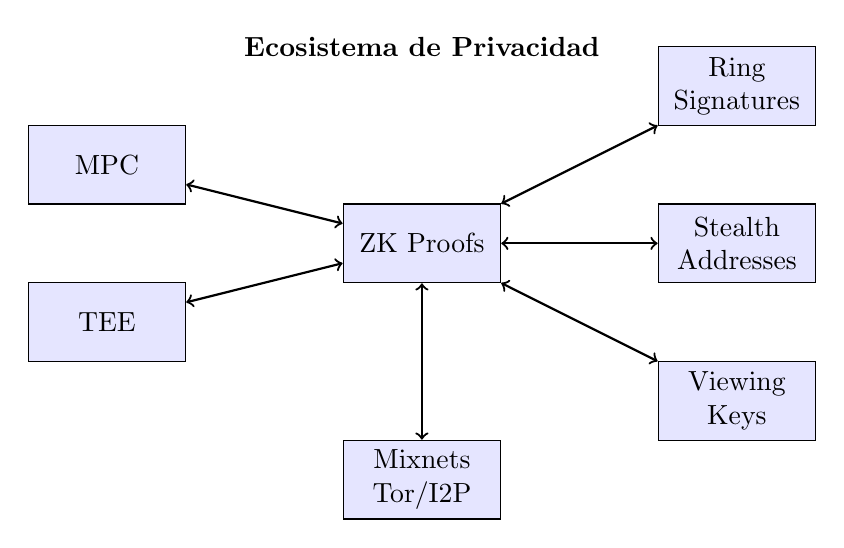
\begin{tikzpicture}[
    tech/.style={draw, rectangle, minimum width=2cm, minimum height=1cm, align=center, fill=blue!10},
    arrow/.style={<->, thick}
]
    % Technologies
    \node[tech] (zk) at (0, 0) {ZK Proofs};
    \node[tech] (ring) at (4, 2) {Ring\\Signatures};
    \node[tech] (stealth) at (4, 0) {Stealth\\Addresses};
    \node[tech] (viewing) at (4, -2) {Viewing\\Keys};
    \node[tech] (mpc) at (-4, 1) {MPC};
    \node[tech] (tee) at (-4, -1) {TEE};
    \node[tech] (mixnet) at (0, -3) {Mixnets\\Tor/I2P};
    
    % Connections
    \draw[arrow] (zk) -- (ring);
    \draw[arrow] (zk) -- (stealth);
    \draw[arrow] (zk) -- (viewing);
    \draw[arrow] (zk) -- (mpc);
    \draw[arrow] (zk) -- (tee);
    \draw[arrow] (zk) -- (mixnet);
    
    % Labels
    \node at (0, 2.5) {\textbf{Ecosistema de Privacidad}};
\end{tikzpicture}
\end{center}

% ============================================
% FIN DEL CAP\'ITULO 3 (CAP 8 ORIGINAL)
% ============================================

% ============================================
% CAP\'ITULO 4: DEFI Y APLICACIONES
% (Cap 9 Original $\to$ Cap 4 Vol 2)
% ============================================

\chapter{DeFi y Aplicaciones}
\label{ch:defi-aplicaciones}

\section*{Introducci\'on}

Las finanzas descentralizadas (DeFi) representan uno de los casos de uso m\'as exitosos de blockchain, permitiendo servicios financieros sin intermediarios tradicionales. Este cap\'itulo explora los protocolos fundamentales de DeFi y su intersecci\'on con tecnolog\'ias de privacidad, especialmente Zero-Knowledge Proofs.

\begin{keyidea}
DeFi replica servicios financieros tradicionales (intercambios, pr\'estamos, derivados) usando smart contracts, eliminando intermediarios y permitiendo composabilidad entre protocolos. La integraci\'on con ZK permite a\~nadir privacidad sin sacrificar auditabilidad.
\end{keyidea}

%===========================================
\section{AMMs (Automated Market Makers)}
\label{sec:amms}
%===========================================

\subsection{Historia y Contexto}

\begin{mathnote}
\textbf{Timeline de AMMs:}
\begin{itemize}
    \item \textbf{2017:} Bancor introduce el primer AMM on-chain
    \item \textbf{2018:} Uniswap v1 simplifica con constant product formula
    \item \textbf{2020:} Uniswap v2 a\~nade pares ERC20/ERC20, flash swaps
    \item \textbf{2020:} Curve optimiza para stablecoins con StableSwap
    \item \textbf{2020:} Balancer generaliza a pools multi-asset
    \item \textbf{2021:} Uniswap v3 introduce concentrated liquidity
    \item \textbf{2023:} Uniswap v4 a\~nade hooks para personalizaci\'on
    \item \textbf{2024+:} AMMs privados con ZK empiezan a emerger
\end{itemize}
\end{mathnote}

\begin{intuicion}
Imagina un mercado tradicional donde compradores y vendedores negocian precios. Un AMM reemplaza esto con una \textbf{f\'ormula matem\'atica} que determina precios autom\'aticamente bas\'andose en las reservas disponibles.

Es como una m\'aquina expendedora infinita: siempre puedes comprar, pero el precio sube cuanto m\'as compras (porque quedan menos). Y siempre puedes vender, pero el precio baja cuanto m\'as vendes (porque hay m\'as disponibles).
\end{intuicion}

\begin{definition}[Automated Market Maker]
Un AMM es un protocolo de intercambio descentralizado que:
\begin{enumerate}
    \item Mantiene \textbf{reservas} de dos o m\'as tokens en un smart contract
    \item Usa una \textbf{funci\'on invariante} $f(x, y, ...) = k$ para determinar precios
    \item Permite intercambios (\textit{swaps}) que modifican reservas manteniendo el invariante
    \item Permite a \textbf{Liquidity Providers (LPs)} depositar/retirar liquidez
\end{enumerate}
\end{definition}

\subsection{Constant Product Formula (Uniswap v2)}

\begin{definition}[Constant Product Market Maker (CPMM)]
El invariante m\'as simple y popular:
\[
x \cdot y = k
\]
donde:
\begin{itemize}
    \item $x$ = reserva del token X
    \item $y$ = reserva del token Y  
    \item $k$ = constante (producto de las reservas)
\end{itemize}
\end{definition}

\subsubsection{Derivaci\'on Matem\'atica del Precio}

\begin{mathnote}
\textbf{Precio Marginal:}

El precio marginal de X en t\'erminos de Y se obtiene de la derivada impl\'icita del invariante:
\[
\frac{d(xy)}{dx} = 0 \implies y + x\frac{dy}{dx} = 0 \implies \frac{dy}{dx} = -\frac{y}{x}
\]
Por tanto, el \textbf{precio spot} de X en t\'erminos de Y es:
\[
P_X = \frac{y}{x}
\]
\end{mathnote}

\begin{example}[C\'alculo de Precio Spot]
Pool ETH/USDC con reservas:
\begin{itemize}
    \item $x = 100$ ETH
    \item $y = 300,000$ USDC
    \item $k = 100 \times 300,000 = 30,000,000$
\end{itemize}

Precio spot de ETH:
\[
P_{ETH} = \frac{300,000}{100} = 3,000 \text{ USDC/ETH}
\]
\end{example}

\subsubsection{F\'ormula de Swap}

\begin{definition}[Swap Output]
Para un swap de $\Delta x$ tokens X, la cantidad de tokens Y recibida es:
\[
\Delta y = \frac{y \cdot \Delta x}{x + \Delta x}
\]

\textbf{Derivaci\'on:}
\begin{align}
x \cdot y &= k \quad \text{(antes del swap)} \\
(x + \Delta x)(y - \Delta y) &= k \quad \text{(despu\'es del swap)} \\
xy - x\Delta y + y\Delta x - \Delta x \Delta y &= xy \\
y\Delta x &= \Delta y(x + \Delta x) \\
\Delta y &= \frac{y \cdot \Delta x}{x + \Delta x}
\end{align}
\end{definition}

\begin{example}[Swap Num\'erico Completo]
Usando el pool anterior (100 ETH, 300,000 USDC), queremos comprar ETH con 3,000 USDC:

\textbf{Paso 1:} Identificar variables
\begin{itemize}
    \item $x = 300,000$ USDC (token que damos)
    \item $y = 100$ ETH (token que recibimos)
    \item $\Delta x = 3,000$ USDC (cantidad que damos)
\end{itemize}

\textbf{Paso 2:} Aplicar f\'ormula
\[
\Delta y = \frac{100 \times 3,000}{300,000 + 3,000} = \frac{300,000}{303,000} \approx 0.9901 \text{ ETH}
\]

\textbf{Paso 3:} Verificar invariante
\begin{itemize}
    \item Antes: $100 \times 300,000 = 30,000,000$
    \item Despu\'es: $(100 - 0.9901) \times (300,000 + 3,000) = 99.0099 \times 303,000 \approx k$
\end{itemize}

\textbf{Paso 4:} Calcular precio efectivo
\[
P_{efectivo} = \frac{3,000}{0.9901} \approx 3,030 \text{ USDC/ETH}
\]

Pagamos \$3,030 por ETH cuando el precio spot era \$3,000 --- la diferencia es el \textbf{slippage}.
\end{example}

\subsubsection{Slippage y Price Impact}

\begin{definition}[Slippage]
La diferencia entre el precio esperado y el precio ejecutado:
\[
\text{Slippage} = \frac{P_{ejecutado} - P_{spot}}{P_{spot}} \times 100\%
\]
\end{definition}

\begin{definition}[Price Impact]
El cambio en el precio spot causado por un trade:
\[
\text{Price Impact} = \frac{\Delta x}{x + \Delta x} \times 100\%
\]

Para el ejemplo anterior:
\[
\text{Price Impact} = \frac{3,000}{303,000} \approx 0.99\%
\]
\end{definition}

\begin{remark}
El slippage aumenta \textbf{cuadr\'aticamente} con el tama\~no del trade relativo al pool. Un trade del 10\% de las reservas tiene $\sim$10\% de price impact. Esto hace que trades grandes en pools peque\~nos sean muy costosos.
\end{remark}

\begin{mathnote}
\textbf{F\'ormula General de Price Impact:}

Para un trade de fracci\'on $\alpha$ de las reservas ($\Delta x = \alpha \cdot x$):
\[
\text{Price Impact} \approx \frac{\alpha}{1 + \alpha} \approx \alpha \quad \text{(para } \alpha \text{ peque\~no)}
\]

\begin{center}
\begin{tabular}{cc}
\toprule
Trade Size ($\alpha$) & Price Impact \\
\midrule
0.1\% & 0.1\% \\
1\% & 0.99\% \\
5\% & 4.76\% \\
10\% & 9.09\% \\
50\% & 33.3\% \\
\bottomrule
\end{tabular}
\end{center}
\end{mathnote}

\subsubsection{Fees en AMMs}

\begin{definition}[Fee Structure (Uniswap v2)]
Uniswap v2 cobra 0.3\% por swap, distribuido a LPs:
\[
\Delta y_{neto} = \frac{y \cdot \Delta x \cdot (1 - \phi)}{x + \Delta x \cdot (1 - \phi)}
\]
donde $\phi = 0.003$ (0.3\%).

Alternativamente, el fee se puede aplicar al output:
\[
\Delta y_{neto} = \Delta y_{bruto} \times (1 - \phi)
\]
\end{definition}

\begin{example}[Swap con Fees]
Mismo ejemplo (3,000 USDC $\to$ ETH):

\textbf{Sin fee:} $\Delta y = 0.9901$ ETH

\textbf{Con fee 0.3\% (aplicado al input):}
\[
\Delta x_{efectivo} = 3,000 \times 0.997 = 2,991 \text{ USDC}
\]
\[
\Delta y = \frac{100 \times 2,991}{300,000 + 2,991} = 0.9871 \text{ ETH}
\]

El LP gana $3,000 - 2,991 = 9$ USDC en fees.
\end{example}

\begin{center}
\begin{tikzpicture}[scale=0.8]
    % Ejes
    \draw[->] (0,0) -- (8,0) node[right] {$x$ (Token A)};
    \draw[->] (0,0) -- (0,8) node[above] {$y$ (Token B)};
    
    % Curva xy = k (k = 16)
    \draw[thick, blue, domain=0.5:7.5, samples=100] 
        plot (\x, {16/\x}) node[right] {$xy = k$};
    
    % Punto inicial
    \fill[red] (4,4) circle (3pt) node[above right] {$(x_0, y_0)$};
    
    % Punto despu\'es del swap
    \fill[green!60!black] (5.33,3) circle (3pt) node[below right] {$(x_1, y_1)$};
    
    % Flechas del swap
    \draw[->, thick, orange] (4,4) -- (5.33,4) node[midway, above] {$+\Delta x$};
    \draw[->, thick, orange] (5.33,4) -- (5.33,3) node[midway, right] {$-\Delta y$};
    
    % L\'ineas de precio (tangentes)
    \draw[dashed, gray] (0,8) -- (8,0);
    
    % Etiquetas de precio
    \node at (2,6) [gray] {Precio alto};
    \node at (6,2) [gray] {Precio bajo};
    
    % Leyenda
    \node[draw, fill=white] at (6,7) {
        \begin{tabular}{l}
        \textcolor{red}{$\bullet$} Antes \\
        \textcolor{green!60!black}{$\bullet$} Despu\'es
        \end{tabular}
    };
\end{tikzpicture}
\end{center}

\subsection{Impermanent Loss}

\begin{definition}[Impermanent Loss (IL)]
La p\'erdida que sufre un LP comparado con simplemente holdear los tokens, causada por cambios en el precio relativo de los tokens.
\end{definition}

\begin{intuicion}
Como LP, siempre est\'as ``vendiendo'' el token que sube y ``comprando'' el que baja para mantener el balance. Si ETH sube 2x mientras eres LP, terminas con menos ETH del que tendr\'ias si solo holdearas.

Se llama ``impermanent'' porque si el precio vuelve al original, la p\'erdida desaparece. Pero si retiras cuando el precio cambi\'o, la p\'erdida se vuelve permanente.
\end{intuicion}

\subsubsection{Derivaci\'on Matem\'atica de IL}

\begin{mathnote}
\textbf{F\'ormula de Impermanent Loss:}

Sea $r = \frac{P_1}{P_0}$ el ratio de cambio de precio. La IL es:
\[
\text{IL}(r) = \frac{2\sqrt{r}}{1 + r} - 1
\]

\textbf{Derivaci\'on:}

Posici\'on inicial: $x_0$ tokens X, $y_0$ tokens Y, precio $P_0 = y_0/x_0$.

Valor inicial: $V_0 = 2 \cdot x_0 \cdot P_0 = 2y_0$ (en t\'erminos de Y).

Despu\'es de cambio de precio a $P_1 = r \cdot P_0$:
\begin{itemize}
    \item Invariante: $x \cdot y = x_0 \cdot y_0 = k$
    \item Nuevo precio: $\frac{y}{x} = r \cdot P_0$
\end{itemize}

Resolviendo:
\begin{align}
\frac{y}{x} &= r \cdot \frac{y_0}{x_0} \\
y &= r \cdot \frac{y_0}{x_0} \cdot x \\
x \cdot r \cdot \frac{y_0}{x_0} \cdot x &= x_0 \cdot y_0 \\
x^2 &= \frac{x_0^2}{r} \\
x_1 &= \frac{x_0}{\sqrt{r}}, \quad y_1 = y_0 \cdot \sqrt{r}
\end{align}

Valor LP despu\'es: $V_{LP} = x_1 \cdot P_1 + y_1 = \frac{x_0}{\sqrt{r}} \cdot r P_0 + y_0\sqrt{r} = 2y_0\sqrt{r}$

Valor HODL: $V_{HODL} = x_0 \cdot P_1 + y_0 = x_0 \cdot r P_0 + y_0 = y_0(r + 1)$

\[
\text{IL} = \frac{V_{LP}}{V_{HODL}} - 1 = \frac{2\sqrt{r}}{1 + r} - 1
\]
\end{mathnote}

\begin{center}
\begin{tabular}{ccc}
\toprule
Cambio de Precio & Ratio $r$ & Impermanent Loss \\
\midrule
-50\% & 0.5 & -5.72\% \\
-25\% & 0.75 & -1.03\% \\
0\% & 1.0 & 0\% \\
+25\% & 1.25 & -0.62\% \\
+50\% & 1.5 & -2.02\% \\
+100\% (2x) & 2.0 & -5.72\% \\
+200\% (3x) & 3.0 & -13.4\% \\
+400\% (5x) & 5.0 & -25.5\% \\
\bottomrule
\end{tabular}
\end{center}

\begin{remark}
La IL es \textbf{sim\'etrica}: un precio que se duplica (2x) o se reduce a la mitad (0.5x) produce la misma IL de $\sim$5.7\%. Esto significa que la volatilidad siempre perjudica al LP, independientemente de la direcci\'on.
\end{remark}

\subsubsection{IL vs Fees: Cu\'ando es Rentable ser LP}

\begin{keyidea}
Un LP es rentable si:
\[
\text{Fees Acumulados} > |\text{Impermanent Loss}|
\]

Para un pool con fee $\phi$ y volumen diario $V$:
\[
\text{APR}_{fees} \approx \frac{\phi \cdot V \cdot 365}{\text{TVL}}
\]

Ejemplo: Pool con TVL = \$10M, Volumen diario = \$5M, Fee = 0.3\%
\[
\text{APR}_{fees} = \frac{0.003 \times 5,000,000 \times 365}{10,000,000} = 54.75\%
\]
\end{keyidea}

\subsection{C\'odigo Solidity: AMM Simplificado}

\begin{example}[Implementaci\'on b\'asica de CPMM]
\begin{verbatim}
// SPDX-License-Identifier: MIT
pragma solidity ^0.8.20;

contract SimpleAMM {
    uint256 public reserveA;
    uint256 public reserveB;
    uint256 public totalSupply;
    
    uint256 public constant FEE_NUMERATOR = 997;
    uint256 public constant FEE_DENOMINATOR = 1000;
    
    function addLiquidity(uint256 amountA, uint256 amountB) 
        external returns (uint256 lpTokens) 
    {
        if (totalSupply == 0) {
            lpTokens = sqrt(amountA * amountB);
        } else {
            uint256 lpFromA = (amountA * totalSupply) / reserveA;
            uint256 lpFromB = (amountB * totalSupply) / reserveB;
            lpTokens = lpFromA < lpFromB ? lpFromA : lpFromB;
        }
        reserveA += amountA;
        reserveB += amountB;
        totalSupply += lpTokens;
    }
    
    function swapAforB(uint256 amountAIn) 
        external returns (uint256 amountBOut) 
    {
        uint256 amountAInWithFee = amountAIn * FEE_NUMERATOR;
        amountBOut = (reserveB * amountAInWithFee) / 
                     (reserveA * FEE_DENOMINATOR + amountAInWithFee);
        reserveA += amountAIn;
        reserveB -= amountBOut;
    }
    
    function sqrt(uint256 x) internal pure returns (uint256 y) {
        if (x == 0) return 0;
        uint256 z = (x + 1) / 2;
        y = x;
        while (z < y) { y = z; z = (x / z + z) / 2; }
    }
}
\end{verbatim}
\end{example}

\begin{bancozk}
\textbf{AMM en Banco ZK:}

El exchange privado de Banco ZK implementa un AMM con privacidad:
\begin{itemize}
    \item \textbf{Montos ocultos:} Los swaps no revelan cantidades exactas
    \item \textbf{Range proofs:} Prueban que el swap es v\'alido sin revelar valores
    \item \textbf{Batching:} M\'ultiples swaps se agregan para aumentar anonymity set
    \item \textbf{Slippage privado:} El usuario especifica slippage m\'aximo en la prueba ZK
\end{itemize}

Circuito de swap privado ($\sim$8,000 constraints):
\begin{verbatim}
template PrivateSwap() {
    signal input amountIn;
    signal input minAmountOut;
    signal input reserveIn;
    signal input reserveOut;
    signal output amountOut;
    signal output nullifier;
    
    // Calcular output
    var amountInWithFee = amountIn * 997;
    amountOut <-- (reserveOut * amountInWithFee) / 
                  (reserveIn * 1000 + amountInWithFee);
    
    // Verificar slippage
    signal slippageOk;
    slippageOk <== GreaterEqThan(64)([amountOut, minAmountOut]);
    slippageOk === 1;
}
\end{verbatim}
\end{bancozk}

\subsection{Concentrated Liquidity (Uniswap v3)}

\begin{definition}[Concentrated Liquidity]
En lugar de distribuir liquidez uniformemente en todo el rango de precios $[0, \infty)$, los LPs concentran su liquidez en un \textbf{rango espec\'ifico} $[p_a, p_b]$.
\end{definition}

\begin{intuicion}
Imagina que eres LP en un pool ETH/USDC. Con Uniswap v2, tu liquidez est\'a distribuida desde precio \$0 hasta $\infty$. Pero ETH probablemente no va a costar \$1 ni \$1,000,000.

Con Uniswap v3, puedes decir: ``Solo quiero proveer liquidez entre \$2,000 y \$4,000''. Esto hace que tu capital sea mucho m\'as eficiente, pero solo ganas fees cuando el precio est\'a en tu rango.
\end{intuicion}

\subsubsection{Matem\'aticas de Concentrated Liquidity}

\begin{mathnote}
\textbf{Liquidez Virtual:}

Uniswap v3 usa el concepto de \textbf{liquidez virtual} $L$:
\[
L = \sqrt{xy}
\]

La f\'ormula constant product se reescribe como:
\[
(x + \frac{L}{\sqrt{p_b}})(y + L\sqrt{p_a}) = L^2
\]

Donde:
\begin{itemize}
    \item $p_a$ = precio inferior del rango
    \item $p_b$ = precio superior del rango
    \item $L$ = liquidez concentrada
\end{itemize}

Para un rango dado, la liquidez real necesaria es:
\[
x_{real} = L \cdot (\frac{1}{\sqrt{p}} - \frac{1}{\sqrt{p_b}})
\]
\[
y_{real} = L \cdot (\sqrt{p} - \sqrt{p_a})
\]
\end{mathnote}

\subsubsection{Ticks en Uniswap v3}

\begin{definition}[Tick]
Un tick es un punto de precio discreto. El precio en tick $i$ es:
\[
p(i) = 1.0001^i
\]

Esto significa que cada tick representa un cambio de precio de 0.01\% (1 basis point).
\end{definition}

\subsubsection{Eficiencia de Capital}

\begin{keyidea}
La eficiencia de capital de concentrated liquidity vs full-range es:
\[
\text{Eficiencia} = \frac{\sqrt{p_b/p_a}}{\sqrt{p_b/p_a} - 1} \cdot \frac{2}{1 + \sqrt{p_a/p_b}}
\]

Para un rango de $\pm$10\% alrededor del precio actual:
\[
\text{Eficiencia} \approx 10x
\]

Esto significa que \$10,000 en un rango estrecho gana los mismos fees que \$100,000 en full-range.
\end{keyidea}

\begin{center}
\begin{tabular}{ccc}
\toprule
Rango & Eficiencia vs Full-Range & Riesgo de salir del rango \\
\midrule
$\pm$50\% & 2.5x & Bajo \\
$\pm$20\% & 5x & Medio \\
$\pm$10\% & 10x & Medio-Alto \\
$\pm$5\% & 20x & Alto \\
$\pm$1\% & 100x & Muy Alto \\
\bottomrule
\end{tabular}
\end{center}

\begin{remark}
\textbf{Riesgo de rangos estrechos:}
\begin{itemize}
    \item Si el precio sale de tu rango, dejas de ganar fees
    \item Tu posici\'on se convierte 100\% en el token depreciado
    \item IL es mayor en rangos estrechos
    \item Requiere gesti\'on activa (rebalanceo)
\end{itemize}
\end{remark}

\subsection{StableSwap (Curve Finance)}

\begin{definition}[StableSwap Invariant]
Curve combina constant product con constant sum para assets de precio similar:
\[
A \cdot n^n \sum x_i + D = A \cdot D \cdot n^n + \frac{D^{n+1}}{n^n \prod x_i}
\]

Donde:
\begin{itemize}
    \item $x_i$ = reserva del token $i$
    \item $n$ = n\'umero de tokens en el pool
    \item $D$ = invariante (total value depositado)
    \item $A$ = amplification coefficient (controla ``planitud'' de la curva)
\end{itemize}
\end{definition}

\begin{intuicion}
\textbf{Constant Sum:} $x + y = k$ --- Precio siempre 1:1, pero se agota un token

\textbf{Constant Product:} $xy = k$ --- Nunca se agota, pero alto slippage

\textbf{StableSwap} interpola entre ambos:
\begin{itemize}
    \item Cuando reservas est\'an balanceadas $\to$ se comporta como constant sum (bajo slippage)
    \item Cuando una reserva se agota $\to$ se comporta como constant product (protege liquidez)
\end{itemize}

El par\'ametro $A$ controla cu\'anto se parece a constant sum. $A$ alto = m\'as plano = menos slippage para stablecoins.
\end{intuicion}

\begin{center}
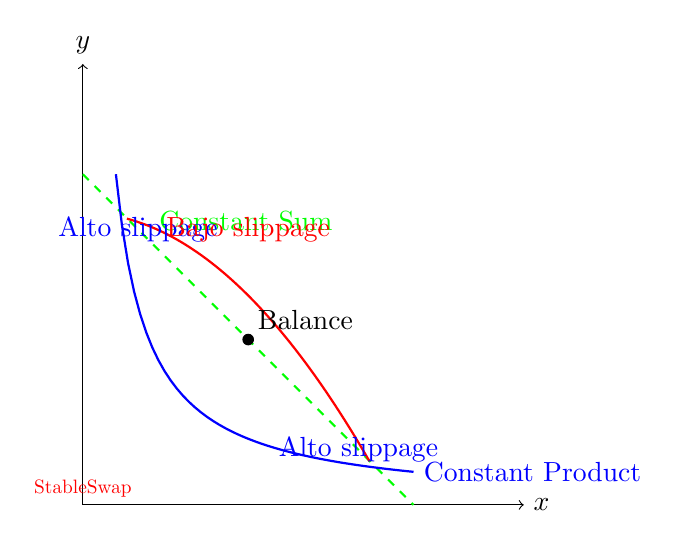
\begin{tikzpicture}[scale=0.7]
    % Ejes
    \draw[->] (0,0) -- (8,0) node[right] {$x$};
    \draw[->] (0,0) -- (0,8) node[above] {$y$};
    
    % Constant Sum (l\'inea recta)
    \draw[thick, green, dashed] (0,6) -- (6,0) node[pos=0.2, above right] {Constant Sum};
    
    % Constant Product (hip\'erbola)
    \draw[thick, blue, domain=0.6:6, samples=50] 
        plot (\x, {3.6/\x}) node[right] {Constant Product};
    
    % StableSwap (intermedio)
    \draw[thick, red, domain=0.8:5.2, samples=50] 
        plot (\x, {6 - \x - 0.5*(\x-3)^2/3 + 0.8}) node[pos=0.8, above] {StableSwap};
    
    % Punto de balance
    \fill (3,3) circle (3pt) node[above right] {Balance};
    
    % Regiones
    \node at (1,5) [blue] {Alto slippage};
    \node at (5,1) [blue] {Alto slippage};
    \node at (3,5) [red] {Bajo slippage};
\end{tikzpicture}
\end{center}

\subsection{Comparativa de AMMs}

\begin{center}
\begin{tabular}{lccccc}
\toprule
\textbf{Protocolo} & \textbf{F\'ormula} & \textbf{Capital Eff.} & \textbf{IL} & \textbf{Mejor para} \\
\midrule
Uniswap v2 & $xy=k$ & Baja & Media & General \\
Uniswap v3 & Concentrated & Alta & Alta & Pares activos \\
Curve v1 & StableSwap & Alta (stables) & Muy baja & Stablecoins \\
Curve v2 & Crypto & Alta & Baja & Pares vol\'atiles \\
Balancer & Weighted & Media & Variable & Portfolios \\
\bottomrule
\end{tabular}
\end{center}

%===========================================
\section{Lending Protocols}
\label{sec:lending}
%===========================================

\subsection{Historia y Contexto}

\begin{mathnote}
\textbf{Timeline de Lending DeFi:}
\begin{itemize}
    \item \textbf{2017:} MakerDAO lanza DAI (CDP model)
    \item \textbf{2018:} Compound introduce cTokens (pool model)
    \item \textbf{2020:} Aave v1 lanza con flash loans
    \item \textbf{2020:} Compound lanza COMP token (liquidity mining)
    \item \textbf{2021:} Aave v2 con credit delegation
    \item \textbf{2022:} Aave v3 con efficiency mode, portals
    \item \textbf{2023:} Morpho (peer-to-peer matching)
    \item \textbf{2024:} Lending privados con ZK empiezan a emerger
\end{itemize}
\end{mathnote}

\begin{definition}[Lending Protocol]
Un protocolo de pr\'estamos DeFi permite:
\begin{enumerate}
    \item \textbf{Depositar} activos y ganar inter\'es
    \item \textbf{Pedir prestado} contra colateral depositado
    \item \textbf{Liquidaci\'on autom\'atica} si el colateral cae
\end{enumerate}
\end{definition}

\begin{intuicion}
Funciona como un banco, pero sin intermediarios:
\begin{itemize}
    \item \textbf{Depositantes} = ahorristas del banco (ganan inter\'es)
    \item \textbf{Prestatarios} = tomadores de cr\'edito (pagan inter\'es)
    \item \textbf{Liquidadores} = cobradores de deuda (ganan bonificaci\'on)
\end{itemize}

La diferencia clave: todo es \textbf{overcollateralized}. No puedes pedir m\'as de lo que depositas. Esto elimina el riesgo de cr\'edito tradicional.
\end{intuicion}

\subsection{Modelo de Tasas de Inter\'es}

\begin{definition}[Utilization Rate]
Proporci\'on del pool que est\'a prestada:
\[
U = \frac{\text{Total Borrowed}}{\text{Total Supplied}}
\]

Ejemplo: Pool de 100M USDC, 70M prestados $\to$ $U = 0.70$ (70\%)
\end{definition}

\begin{definition}[Interest Rate Model (Compound-style)]
La tasa de inter\'es es funci\'on de la utilizaci\'on:

\textbf{Modelo b\'asico (lineal):}
\[
R_{borrow} = R_{base} + U \cdot R_{slope}
\]

\textbf{Modelo con ``kink'' (Compound/Aave):}
\[
R_{borrow} = \begin{cases}
R_{base} + U \cdot R_{slope1} & \text{si } U \leq U_{optimal} \\
R_{base} + U_{optimal} \cdot R_{slope1} + (U - U_{optimal}) \cdot R_{slope2} & \text{si } U > U_{optimal}
\end{cases}
\]

Donde $R_{slope2} \gg R_{slope1}$ para desincentivar alta utilizaci\'on.
\end{definition}

\begin{center}
\begin{tikzpicture}[scale=0.8]
    % Ejes
    \draw[->] (0,0) -- (10,0) node[right] {Utilization (\%)};
    \draw[->] (0,0) -- (0,8) node[above] {Borrow Rate (\%)};
    
    % Modelo con kink
    \draw[thick, blue] (0,0.5) -- (8,2.5);
    \draw[thick, blue] (8,2.5) -- (10,7);
    
    % Kink point
    \fill[red] (8,2.5) circle (3pt);
    \node at (8,3) [above] {Kink (80\%)};
    
    % Etiquetas
    \node at (2,-0.5) {20\%};
    \node at (4,-0.5) {40\%};
    \node at (6,-0.5) {60\%};
    \node at (8,-0.5) {80\%};
    \node at (10,-0.5) {100\%};
    
    \node at (-0.5,0.5) {2\%};
    \node at (-0.5,2.5) {10\%};
    \node at (-0.5,7) {50\%};
    
    % Anotaciones
    \draw[dashed, gray] (8,0) -- (8,2.5);
    \node at (4,1) {Slope1 (bajo)};
    \node at (9,5) [rotate=70] {Slope2 (alto)};
\end{tikzpicture}
\end{center}

\subsection{Colateralizaci\'on y Liquidaciones}

\begin{definition}[Loan-to-Value (LTV)]
Ratio m\'aximo que puedes pedir prestado contra tu colateral:
\[
\text{Max Borrow} = \text{Collateral Value} \times \text{LTV}
\]

Ejemplo: LTV de ETH = 80\%. Con \$10,000 en ETH, puedes pedir hasta \$8,000.
\end{definition}

\begin{definition}[Health Factor]
Medida de ``salud'' de una posici\'on:
\[
HF = \frac{\sum(\text{Collateral}_i \times \text{LiqThreshold}_i)}{\text{Total Borrowed}}
\]

\begin{itemize}
    \item $HF > 1$: Posici\'on segura
    \item $HF = 1$: En el l\'imite de liquidaci\'on
    \item $HF < 1$: Puede ser liquidada
\end{itemize}
\end{definition}

\begin{example}[Escenario de Liquidaci\'on]
\textbf{Posici\'on inicial:}
\begin{itemize}
    \item Colateral: 10 ETH @ \$3,000 = \$30,000
    \item Prestado: \$20,000 USDC
    \item Liquidation Threshold ETH: 82.5\%
\end{itemize}

\[
HF = \frac{30,000 \times 0.825}{20,000} = 1.2375
\]

\textbf{ETH cae a \$2,400:}
\[
HF = \frac{24,000 \times 0.825}{20,000} = 0.99
\]

La posici\'on puede ser liquidada. Un liquidador:
\begin{enumerate}
    \item Paga hasta \$10,000 USDC (50\% de la deuda, l\'imite t\'ipico)
    \item Recibe ETH equivalente + bonificaci\'on (5\%)
    \item Recibe: $\frac{10,000 \times 1.05}{2,400} = 4.375$ ETH
\end{enumerate}
\end{example}

\begin{remark}
\textbf{Riesgos de Lending:}
\begin{itemize}
    \item \textbf{Smart contract risk:} Bugs en el c\'odigo
    \item \textbf{Oracle manipulation:} Precios incorrectos $\to$ liquidaciones incorrectas
    \item \textbf{Liquidation cascade:} Liquidaciones masivas causan m\'as liquidaciones
    \item \textbf{Bad debt:} Si el precio cae muy r\'apido, la liquidaci\'on puede no cubrir la deuda
    \item \textbf{Governance attacks:} Cambios maliciosos en par\'ametros
\end{itemize}
\end{remark}

\subsection{Flash Loans}

\begin{definition}[Flash Loan]
Pr\'estamo \textbf{sin colateral} que debe ser devuelto en la \textbf{misma transacci\'on}. Si no se devuelve, toda la transacci\'on revierte.
\end{definition}

\begin{intuicion}
Un flash loan es como pedir prestado \$10 millones por 13 segundos (un bloque). Puedes hacer lo que quieras con ese dinero, pero \textit{debes} devolverlo antes de que termine la transacci\'on.

Es posible porque en blockchain todo es at\'omico: o la transacci\'on completa sucede, o nada sucede. No hay estado intermedio donde el protocolo ``pierde'' el dinero.
\end{intuicion}

\subsubsection{Casos de Uso de Flash Loans}

\begin{enumerate}
    \item \textbf{Arbitraje:}
    \begin{itemize}
        \item Pedir prestado USDC
        \item Comprar ETH barato en DEX A
        \item Vender ETH caro en DEX B
        \item Devolver USDC + fee, quedarse con ganancia
    \end{itemize}
    
    \item \textbf{Liquidaciones:}
    \begin{itemize}
        \item Pedir prestado USDC para pagar deuda de otro usuario
        \item Recibir colateral con bonificaci\'on
        \item Vender colateral, devolver flash loan
    \end{itemize}
    
    \item \textbf{Collateral Swap:}
    \begin{itemize}
        \item Pedir prestado para pagar tu propia deuda
        \item Retirar colateral (ETH)
        \item Cambiar ETH por otro activo (BTC)
        \item Depositar nuevo colateral
        \item Pedir prestado de nuevo para devolver flash loan
    \end{itemize}
    
    \item \textbf{Self-liquidation:}
    \begin{itemize}
        \item Evitar pagar bonificaci\'on al liquidador
        \item Usar flash loan para cerrar posici\'on uno mismo
    \end{itemize}
\end{enumerate}

\begin{bancozk}
\textbf{Lending Privado en Banco ZK:}

Banco ZK implementa lending con privacidad parcial:

\begin{itemize}
    \item \textbf{Montos ocultos:} El p\'ublico no ve cu\'anto depositas/pides prestado
    \item \textbf{Health Factor verificable:} ZK proof de que $HF > 1$ sin revelar valores exactos
    \item \textbf{Liquidaciones privadas:} Solo el liquidador sabe el monto exacto
    \item \textbf{Tasas p\'ublicas:} Las tasas de inter\'es son p\'ublicas para transparencia
\end{itemize}

Circuito de verificaci\'on de Health Factor ($\sim$5,000 constraints):
\begin{verbatim}
template HealthFactorCheck() {
    signal input collateralValue;
    signal input borrowedValue;
    signal input liqThreshold;  // e.g., 8250 para 82.5%
    signal output isHealthy;  // 1 si HF > 1
    
    signal numerator;
    numerator <== collateralValue * liqThreshold;
    
    signal denominator;
    denominator <== borrowedValue * 10000;
    
    isHealthy <== GreaterThan(128)([numerator, denominator]);
}
\end{verbatim}
\end{bancozk}

%===========================================
\section{Or\'aculos}
\label{sec:oracles}
%===========================================

\subsection{El Problema del Or\'aculo}

\begin{definition}[Oracle Problem]
Las blockchains son sistemas deterministas cerrados: no pueden acceder a datos externos de forma nativa. Un \textbf{or\'aculo} es un mecanismo para traer datos del mundo real a la blockchain de forma confiable.
\end{definition}

\begin{intuicion}
Imagina un smart contract de seguros agr\'icolas que paga si llueve menos de 50mm en un mes. El contrato necesita saber cu\'anto llovi\'o, pero esa informaci\'on est\'a ``fuera'' de la blockchain.

El problema es: ?`c\'omo confiar en quien reporta la lluvia? Si una sola persona lo reporta, puede mentir. Si es un grupo, pueden coludirse. Los or\'aculos intentan resolver esto con incentivos econ\'omicos y descentralizaci\'on.
\end{intuicion}

\begin{remark}
\textbf{``Garbage In, Garbage Out'':}

Un smart contract es tan seguro como sus or\'aculos. Un contrato perfectamente auditado puede ser explotado si el or\'aculo reporta precios incorrectos.

Ejemplos hist\'oricos:
\begin{itemize}
    \item \textbf{Mango Markets (2022):} Manipulaci\'on de precio para pedir pr\'estamos excesivos (\$114M)
    \item \textbf{Cream Finance (2021):} Oracle manipulation, \$130M robados
    \item \textbf{Harvest Finance (2020):} Flash loan + oracle manipulation, \$34M
\end{itemize}
\end{remark}

\subsection{Tipos de Or\'aculos}

\begin{definition}[Clasificaci\'on de Or\'aculos]
\textbf{Por direcci\'on del flujo:}
\begin{itemize}
    \item \textbf{Inbound:} Traen datos externos $\to$ blockchain (precios, clima)
    \item \textbf{Outbound:} Env\'ian datos blockchain $\to$ mundo externo (triggers)
\end{itemize}

\textbf{Por arquitectura:}
\begin{itemize}
    \item \textbf{Centralizados:} Una entidad provee datos (simple pero single point of failure)
    \item \textbf{Descentralizados:} Red de nodos con consenso (Chainlink, Band)
    \item \textbf{On-chain:} Calculados de datos on-chain (TWAP de AMMs)
\end{itemize}

\textbf{Por tipo de dato:}
\begin{itemize}
    \item \textbf{Price feeds:} Precios de activos
    \item \textbf{VRF:} Aleatoriedad verificable
    \item \textbf{Proof of Reserve:} Verificaci\'on de reservas off-chain
    \item \textbf{Cross-chain:} Estado de otras blockchains
\end{itemize}
\end{definition}

\subsection{Chainlink}

\begin{definition}[Chainlink]
Red descentralizada de or\'aculos con:
\begin{itemize}
    \item \textbf{Nodos operadores:} Proveen datos y staking
    \item \textbf{Aggregation:} M\'ultiples fuentes, mediana como resultado
    \item \textbf{Reputation:} Sistema de reputaci\'on basado en historial
    \item \textbf{LINK token:} Para pagos y staking
\end{itemize}
\end{definition}

\begin{center}
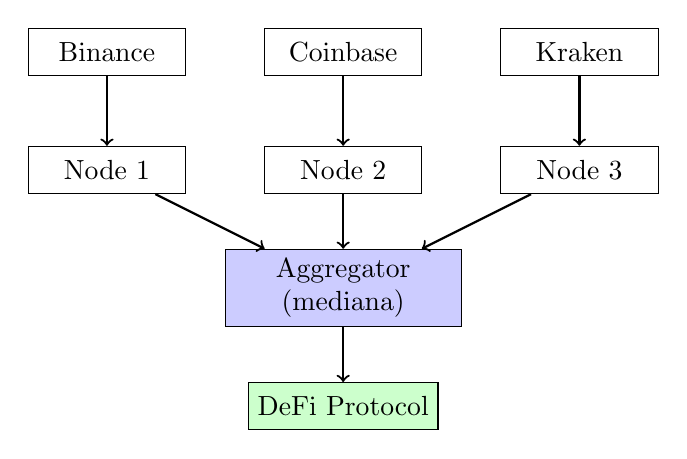
\begin{tikzpicture}[
    node distance=1.5cm,
    box/.style={draw, rectangle, minimum width=2cm, minimum height=0.6cm, align=center},
    arrow/.style={->, thick}
]
    % Data Sources
    \node[box] (src1) at (0,3) {Binance};
    \node[box] (src2) at (3,3) {Coinbase};
    \node[box] (src3) at (6,3) {Kraken};
    
    % Nodos
    \node[box] (node1) at (0,1.5) {Node 1};
    \node[box] (node2) at (3,1.5) {Node 2};
    \node[box] (node3) at (6,1.5) {Node 3};
    
    % Aggregator
    \node[box, fill=blue!20, minimum width=3cm] (agg) at (3,0) {Aggregator\\(mediana)};
    
    % Consumer
    \node[box, fill=green!20] (consumer) at (3,-1.5) {DeFi Protocol};
    
    % Flechas
    \draw[arrow] (src1) -- (node1);
    \draw[arrow] (src2) -- (node2);
    \draw[arrow] (src3) -- (node3);
    
    \draw[arrow] (node1) -- (agg);
    \draw[arrow] (node2) -- (agg);
    \draw[arrow] (node3) -- (agg);
    
    \draw[arrow] (agg) -- (consumer);
\end{tikzpicture}
\end{center}

\subsection{TWAP (Time-Weighted Average Price)}

\begin{definition}[TWAP]
Precio promedio ponderado por tiempo, calculado de datos on-chain (t\'ipicamente de un AMM):
\[
\text{TWAP}_{t_1 \to t_2} = \frac{1}{t_2 - t_1} \int_{t_1}^{t_2} P(t) \, dt
\]

En pr\'actica, usando acumuladores:
\[
\text{TWAP} = \frac{\text{cumulative}_{t_2} - \text{cumulative}_{t_1}}{t_2 - t_1}
\]

Donde $\text{cumulative}_t = \sum_{i=0}^{t} P_i \cdot \Delta t_i$
\end{definition}

\begin{intuicion}
TWAP es m\'as resistente a manipulaci\'on que el precio spot porque un atacante necesitar\'ia mantener el precio manipulado durante todo el per\'iodo TWAP, lo cual es costoso.

Si el TWAP es de 30 minutos y un atacante manipula el precio por 1 minuto, solo afecta 1/30 del TWAP final.
\end{intuicion}

\subsection{Manipulaci\'on de Or\'aculos}

\begin{definition}[Oracle Manipulation Attack]
Ataque donde el adversario manipula el precio reportado por un or\'aculo para explotar un protocolo DeFi.
\end{definition}

\subsubsection{Vectores de Ataque}

\begin{enumerate}
    \item \textbf{Flash Loan + AMM Manipulation:}
    \begin{itemize}
        \item Pedir flash loan masivo
        \item Swap grande para mover precio del AMM
        \item Protocolo v\'ictima lee precio manipulado
        \item Explotar (pedir pr\'estamo excesivo, liquidar incorrectamente)
        \item Revertir swap, devolver flash loan
    \end{itemize}
    
    \item \textbf{Sandwich de Or\'aculo:}
    \begin{itemize}
        \item Detectar actualizaci\'on de or\'aculo pendiente
        \item Front-run con transacci\'on que se beneficia del precio viejo
        \item Dejar que el or\'aculo actualice
        \item Back-run para cerrar posici\'on con precio nuevo
    \end{itemize}
    
    \item \textbf{Stale Price:}
    \begin{itemize}
        \item Explotar cuando el or\'aculo no se actualiza
        \item Precio on-chain difiere significativamente del real
        \item Arbitrar la diferencia
    \end{itemize}
\end{enumerate}

\subsubsection{Defensas}

\begin{keyidea}
\textbf{Best Practices para Or\'aculos:}
\begin{enumerate}
    \item \textbf{TWAP > Spot:} Usar precios promediados, no instant\'aneos
    \item \textbf{M\'ultiples fuentes:} No depender de un solo or\'aculo
    \item \textbf{Sanity checks:} Verificar que el precio est\'a en rango razonable
    \item \textbf{Freshness checks:} Rechazar precios muy viejos
    \item \textbf{Circuit breakers:} Pausar protocolo si hay anomal\'ias
    \item \textbf{Delays:} Introducir delays para hacer ataques m\'as costosos
\end{enumerate}
\end{keyidea}

\subsection{Chainlink VRF (Verifiable Random Function)}

\begin{definition}[VRF]
Funci\'on que genera n\'umeros aleatorios con prueba criptogr\'afica de que fueron generados correctamente. Propiedades:
\begin{itemize}
    \item \textbf{Unpredictable:} Nadie puede predecir el resultado antes de generarlo
    \item \textbf{Verifiable:} Cualquiera puede verificar que el resultado es correcto
    \item \textbf{Deterministic:} La misma entrada siempre produce la misma salida
\end{itemize}
\end{definition}

\begin{bancozk}
\textbf{Or\'aculos en Banco ZK:}

Banco ZK usa un dise\~no h\'ibrido de or\'aculos:

\begin{itemize}
    \item \textbf{Precios p\'ublicos:} Chainlink para ETH/USD (no hay raz\'on para ocultar)
    \item \textbf{Verificaci\'on privada:} ZK proofs que verifican condiciones sin revelar valores
    \item \textbf{TWAP privado:} Acumuladores cifrados para TWAP que no revela trades individuales
\end{itemize}

Ejemplo: Verificar que un pr\'estamo est\'a healthy sin revelar el monto:
\begin{verbatim}
template OracleBasedHealthCheck() {
    signal input collateralAmount;     // Privado
    signal input oraclePrice;          // P\'ublico (de Chainlink)
    signal input borrowedAmount;       // Privado
    signal input liquidationThreshold; // P\'ublico
    signal output isHealthy;
    
    signal collateralValue;
    collateralValue <== collateralAmount * oraclePrice;
    
    signal threshold_x_collateral;
    threshold_x_collateral <== collateralValue * liquidationThreshold;
    
    signal threshold_x_borrowed;
    threshold_x_borrowed <== borrowedAmount * 10000;
    
    isHealthy <== GreaterThan(128)(
        [threshold_x_collateral, threshold_x_borrowed]
    );
}
\end{verbatim}

Esto permite que Banco ZK use precios de mercado p\'ublicos mientras mantiene los montos de los usuarios privados.
\end{bancozk}

%===========================================
\section{Bridges ZK}
\label{sec:zkbridges}
%===========================================

\subsection{El Problema de los Bridges}

\begin{definition}[Blockchain Bridge]
Protocolo que permite transferir activos o mensajes entre dos blockchains diferentes.
\end{definition}

\begin{intuicion}
Las blockchains son ``islas'' aisladas. Bitcoin no sabe nada de Ethereum, y viceversa. Un bridge es como un ferry que lleva activos de una isla a otra.

El problema es: ?`c\'omo confiar en el ferry? Si el operador del ferry dice ``te doy 1 ETH en Ethereum porque bloqueaste 1 ETH en otra cadena'', ?`c\'omo verificamos que realmente lo hizo?
\end{intuicion}

\subsubsection{Modelos de Bridges Tradicionales}

\begin{center}
\begin{tabular}{lccc}
\toprule
\textbf{Modelo} & \textbf{Trust} & \textbf{Seguridad} & \textbf{Ejemplos} \\
\midrule
Custodial & Centralizado & Baja & WBTC \\
Multisig & $n$-of-$m$ & Media & Multichain \\
MPC & Threshold & Media-Alta & Thorchain \\
Optimistic & Fraud proofs & Alta & Nomad \\
\textbf{ZK} & \textbf{Math} & \textbf{Muy Alta} & \textbf{Succinct, zkBridge} \\
\bottomrule
\end{tabular}
\end{center}

\begin{remark}
\textbf{Historial de Hacks en Bridges:}
\begin{itemize}
    \item \textbf{Ronin (2022):} \$624M --- Multisig comprometido
    \item \textbf{Wormhole (2022):} \$320M --- Bug en verificaci\'on de firmas
    \item \textbf{Nomad (2022):} \$190M --- Bug en verificaci\'on de merkle proofs
    \item \textbf{Multichain (2023):} \$126M --- CEO detenido, claves comprometidas
\end{itemize}

M\'as de \$2B robados de bridges. Son el eslab\'on m\'as d\'ebil del ecosistema multi-chain.
\end{remark}

\subsection{ZK Bridges: Verificaci\'on Criptogr\'afica}

\begin{definition}[ZK Bridge]
Bridge que verifica la validez de transacciones cross-chain usando \textbf{pruebas de conocimiento cero}, eliminando la necesidad de confiar en operadores.
\end{definition}

\begin{keyidea}
La idea central de un ZK bridge es:

\textit{``No conf\'ies en que el operador dice la verdad. Verifica una prueba matem\'atica de que la transacci\'on realmente ocurri\'o en la cadena origen.''}

Esto convierte el problema de confianza en un problema de criptograf\'ia, que es mucho m\'as seguro.
\end{keyidea}

\subsubsection{Arquitectura de ZK Bridge}

\begin{center}
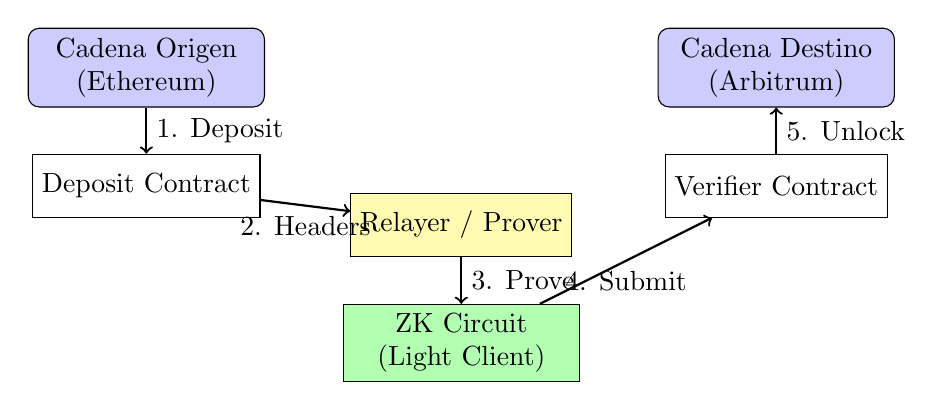
\begin{tikzpicture}[
    node distance=1.2cm,
    box/.style={draw, rectangle, minimum width=2.5cm, minimum height=0.8cm, align=center},
    chain/.style={draw, rectangle, rounded corners, minimum width=3cm, minimum height=1cm, align=center, fill=blue!20},
    arrow/.style={->, thick}
]
    % Cadenas
    \node[chain] (chainA) at (0,0) {Cadena Origen\\(Ethereum)};
    \node[chain] (chainB) at (8,0) {Cadena Destino\\(Arbitrum)};
    
    % Componentes
    \node[box] (deposit) at (0,-1.5) {Deposit Contract};
    \node[box, fill=yellow!30] (relayer) at (4,-2) {Relayer / Prover};
    \node[box] (verifier) at (8,-1.5) {Verifier Contract};
    
    % ZK Circuit
    \node[box, fill=green!30, minimum width=3cm] (circuit) at (4,-3.5) {ZK Circuit\\(Light Client)};
    
    % Flujo
    \draw[arrow] (chainA) -- (deposit) node[midway, right] {1. Deposit};
    \draw[arrow] (deposit) -- (relayer) node[midway, below] {2. Headers};
    \draw[arrow] (relayer) -- (circuit) node[midway, right] {3. Prove};
    \draw[arrow] (circuit) -- (verifier) node[midway, below] {4. Submit};
    \draw[arrow] (verifier) -- (chainB) node[midway, right] {5. Unlock};
\end{tikzpicture}
\end{center}

\subsubsection{Componentes del ZK Bridge}

\begin{definition}[Light Client en ZK]
Un circuito ZK que verifica el consenso de una blockchain sin procesar todos los bloques:
\begin{enumerate}
    \item \textbf{Verificar firmas de validadores:} Probar que $\geq 2/3$ de validadores firmaron el bloque
    \item \textbf{Verificar transici\'on de estado:} Block hash anterior $\to$ Block hash actual
    \item \textbf{Verificar inclusi\'on:} Merkle proof de que la transacci\'on est\'a en el bloque
\end{enumerate}
\end{definition}

\begin{mathnote}
\textbf{Complejidad de Light Client ZK:}

Para Ethereum PoS:
\begin{itemize}
    \item \textbf{Sync Committee:} 512 validadores por per\'iodo (256 epochs)
    \item \textbf{Firmas BLS:} Agregaci\'on permite verificar 512 firmas como una
    \item \textbf{Merkle Proofs:} $\sim$20 hashes para verificar inclusi\'on
\end{itemize}

Circuito t\'ipico: 1-10M constraints
\begin{itemize}
    \item BLS signature verification: $\sim$500K constraints per signature
    \item BLS aggregation check: $\sim$2M constraints
    \item Merkle proof (SHA256, 20 levels): $\sim$200K constraints
    \item State root verification: $\sim$100K constraints
\end{itemize}

Tiempo de proving: 30 segundos - 5 minutos (dependiendo del hardware)
\end{mathnote}

\subsection{Proyectos de ZK Bridges}

\begin{center}
\begin{tabular}{lcccc}
\toprule
\textbf{Proyecto} & \textbf{Tecnolog\'ia} & \textbf{Cadenas} & \textbf{Tiempo Proof} & \textbf{Estado} \\
\midrule
Succinct & SP1 (zkVM) & Ethereum + & $\sim$2 min & Mainnet \\
zkBridge & deVirgo & ETH, Cosmos & $\sim$5 min & Testnet \\
Lagrange & Custom ZK & Multi-chain & $\sim$1 min & Mainnet \\
Polyhedra & Expander & 20+ chains & $\sim$30 sec & Mainnet \\
\bottomrule
\end{tabular}
\end{center}

\subsection{Desaf\'ios y Limitaciones}

\begin{remark}
\textbf{Desaf\'ios actuales de ZK Bridges:}

\begin{enumerate}
    \item \textbf{Costo de proving:}
    \begin{itemize}
        \item Generar pruebas requiere hardware potente
        \item \$0.10 - \$10 por prueba dependiendo del circuito
        \item Amortizado si hay volumen
    \end{itemize}
    
    \item \textbf{Latencia:}
    \begin{itemize}
        \item 30 segundos - 5 minutos para generar prueba
        \item + tiempo de inclusi\'on en ambas cadenas
        \item Total: 5-30 minutos vs segundos en bridges tradicionales
    \end{itemize}
    
    \item \textbf{Complejidad de consenso:}
    \begin{itemize}
        \item Cada blockchain tiene consenso diferente
        \item Cambios en el protocolo requieren actualizar circuitos
        \item BLS signatures son costosas en ZK
    \end{itemize}
    
    \item \textbf{Ataques de reorganizaci\'on:}
    \begin{itemize}
        \item ?`Qu\'e pasa si la cadena origen hace reorg despu\'es del bridge?
        \item Necesita esperar finalidad (12+ minutos en Ethereum)
    \end{itemize}
\end{enumerate}
\end{remark}

\begin{bancozk}
\textbf{ZK Bridge de Banco ZK:}

Banco ZK implementa un bridge nativo a Ethereum L1 con las siguientes caracter\'isticas:

\begin{itemize}
    \item \textbf{Deposits (L1 $\to$ L2):}
    \begin{enumerate}
        \item Usuario deposita en contrato L1
        \item Secuenciador de Banco ZK detecta el dep\'osito
        \item Genera commitment a la nota privada
        \item Usuario puede gastar en L2 con prueba de inclusi\'on
    \end{enumerate}
    
    \item \textbf{Withdrawals (L2 $\to$ L1):}
    \begin{enumerate}
        \item Usuario genera prueba ZK de posesi\'on de nota
        \item Prueba se incluye en batch de L2
        \item Proof agregado se verifica en L1
        \item Usuario reclama fondos en L1
    \end{enumerate}
    
    \item \textbf{Tiempos:}
    \begin{itemize}
        \item Deposit: 12 minutos (finalidad ETH) + 1 minuto (procesamiento)
        \item Withdrawal: Inmediato con prueba v\'alida (no hay dispute period)
    \end{itemize}
    
    \item \textbf{Privacidad del bridge:}
    \begin{itemize}
        \item Deposits en L1 son p\'ublicos (necesario)
        \item Actividad en L2 es privada
        \item Withdrawals revelan monto pero no historial
    \end{itemize}
\end{itemize}
\end{bancozk}

%===========================================
\section{Atomic Swaps}
\label{sec:atomicswaps}
%===========================================

\subsection{Fundamentos}

\begin{definition}[Atomic Swap]
Intercambio de activos entre dos blockchains sin intermediarios, con garant\'ia de que:
\begin{itemize}
    \item Ambas partes reciben sus fondos, o
    \item Ninguna parte pierde sus fondos (transacci\'on revierte)
\end{itemize}

La ``atomicidad'' significa: todo o nada.
\end{definition}

\begin{intuicion}
Imagina que quieres cambiar 1 BTC por 30 ETH con un desconocido en internet:
\begin{itemize}
    \item Si env\'ias primero, pueden no enviarte ETH
    \item Si ellos env\'ian primero, puedes no enviarles BTC
\end{itemize}

Un atomic swap usa criptograf\'ia para crear un ``acuerdo'' donde ambas transferencias est\'an vinculadas por un secreto. Quien revela el secreto para cobrar en una cadena, autom\'aticamente permite que la otra parte cobre en la otra cadena.
\end{intuicion}

\subsection{HTLC (Hash Time-Locked Contracts)}

\begin{definition}[HTLC]
Contrato que bloquea fondos con dos condiciones de desbloqueo:
\begin{enumerate}
    \item \textbf{Hashlock:} Revelar preimagen $s$ tal que $H(s) = h$
    \item \textbf{Timelock:} Esperar hasta tiempo $t$ (refund)
\end{enumerate}
\end{definition}

\subsubsection{Protocolo de Atomic Swap con HTLC}

\begin{mathnote}
\textbf{Protocolo Detallado:}

\textbf{Setup:}
\begin{itemize}
    \item Alice quiere: 30 ETH (tiene 1 BTC)
    \item Bob quiere: 1 BTC (tiene 30 ETH)
    \item Acuerdan precio: 1 BTC = 30 ETH
\end{itemize}

\textbf{Paso 1: Alice genera secreto}
\begin{itemize}
    \item $s \leftarrow \{0,1\}^{256}$ (256 bits aleatorios)
    \item $h = \text{SHA256}(s)$
    \item Alice env\'ia $h$ a Bob (NO el secreto $s$)
\end{itemize}

\textbf{Paso 2: Alice bloquea en Bitcoin}
\begin{itemize}
    \item Crea HTLC: ``1 BTC para quien revele $s$ tal que $H(s) = h$, o devolver a Alice despu\'es de 48 horas''
    \item Publica transacci\'on en Bitcoin
\end{itemize}

\textbf{Paso 3: Bob verifica y bloquea en Ethereum}
\begin{itemize}
    \item Bob verifica que el HTLC de Alice es correcto
    \item Crea HTLC: ``30 ETH para quien revele $s$ tal que $H(s) = h$, o devolver a Bob despu\'es de 24 horas''
    \item El timelock de Bob (24h) es MENOR que el de Alice (48h)
\end{itemize}

\textbf{Paso 4: Alice reclama ETH}
\begin{itemize}
    \item Alice revela $s$ en Ethereum para reclamar 30 ETH
    \item Al hacerlo, $s$ se vuelve p\'ublico (visible en blockchain)
\end{itemize}

\textbf{Paso 5: Bob reclama BTC}
\begin{itemize}
    \item Bob ve $s$ en la transacci\'on de Alice
    \item Bob usa $s$ en Bitcoin para reclamar 1 BTC
    \item Tiene 24+ horas para hacerlo (48h - 24h = 24h de margen)
\end{itemize}
\end{mathnote}

\subsection{Limitaciones de HTLC}

\begin{remark}
\textbf{Problemas de Atomic Swaps con HTLC:}

\begin{enumerate}
    \item \textbf{Tiempos largos:}
    \begin{itemize}
        \item Necesita esperar confirmaciones en ambas cadenas
        \item Timelocks de 24-48 horas t\'ipicos
        \item No es pr\'actico para trading frecuente
    \end{itemize}
    
    \item \textbf{Problema de ``Free Option'':}
    \begin{itemize}
        \item Alice puede esperar hasta el \'ultimo momento
        \item Si el precio se mueve a su favor, reclama
        \item Si el precio se mueve en contra, deja expirar
        \item Bob queda ``atrapado'' durante el timelock
    \end{itemize}
    
    \item \textbf{Requiere ambas partes online:}
    \begin{itemize}
        \item Bob debe monitorear para ver cuando Alice revela $s$
        \item Si Bob est\'a offline, puede perder la ventana de reclamo
    \end{itemize}
    
    \item \textbf{No soporta todas las cadenas:}
    \begin{itemize}
        \item Requiere scripting (hashlocks, timelocks)
        \item Bitcoin s\'i, pero algunas cadenas no
    \end{itemize}
\end{enumerate}
\end{remark}

%===========================================
\section{Cross-chain Interoperability}
\label{sec:crosschain}
%===========================================

\subsection{Protocolos de Messaging}

\begin{definition}[Cross-chain Messaging]
Protocolos que permiten enviar mensajes arbitrarios entre blockchains, no solo transferencias de valor.
\end{definition}

\subsubsection{IBC (Inter-Blockchain Communication)}

\begin{definition}[IBC]
Protocolo de Cosmos para comunicaci\'on entre blockchains:
\begin{itemize}
    \item \textbf{Light Clients:} Cada cadena mantiene light client de las otras
    \item \textbf{Relayers:} Transmiten paquetes entre cadenas
    \item \textbf{Canales:} Conexiones ordenadas entre m\'odulos
    \item \textbf{Timeout:} Garant\'ia de entrega o reembolso
\end{itemize}
\end{definition}

\subsubsection{LayerZero}

\begin{definition}[LayerZero]
Protocolo de messaging cross-chain con:
\begin{itemize}
    \item \textbf{Ultra Light Nodes:} Light clients on-demand
    \item \textbf{Oracles:} Reportan block headers
    \item \textbf{Relayers:} Transmiten proofs de transacciones
    \item \textbf{Modular security:} Apps eligen oracles/relayers
\end{itemize}
\end{definition}

\subsubsection{Axelar y Wormhole}

\begin{definition}[Axelar]
Red de validadores para general message passing:
\begin{itemize}
    \item \textbf{Proof-of-Stake:} Validadores con AXL staked
    \item \textbf{Threshold signatures:} Firma colectiva para aprobar mensajes
    \item \textbf{Gateway contracts:} En cada cadena conectada
    \item \textbf{GMP:} General Message Passing
\end{itemize}
\end{definition}

\begin{definition}[Wormhole]
Protocolo cross-chain con Guardians:
\begin{itemize}
    \item \textbf{19 Guardians:} Nodos que observan todas las cadenas
    \item \textbf{VAAs:} Verified Action Approvals (mensajes firmados)
    \item \textbf{13/19 threshold:} Se requieren 13 firmas para aprobar
    \item \textbf{24+ cadenas:} Ethereum, Solana, BSC, etc.
\end{itemize}
\end{definition}

\subsection{Comparativa de Protocolos Cross-chain}

\begin{center}
\begin{tabular}{lcccc}
\toprule
\textbf{Protocolo} & \textbf{Modelo} & \textbf{Seguridad} & \textbf{Cadenas} & \textbf{Latencia} \\
\midrule
IBC & Light clients & Muy alta & Cosmos & $\sim$20 sec \\
LayerZero & Oracle + Relayer & Configurable & 50+ & $\sim$2 min \\
Axelar & PoS validators & Alta & 40+ & $\sim$2 min \\
Wormhole & Multisig (19) & Media-Alta & 24+ & $\sim$15 min \\
Hyperlane & Modular & Configurable & 30+ & Variable \\
CCIP & DON network & Alta & 10+ & $\sim$20 min \\
\bottomrule
\end{tabular}
\end{center}

%===========================================
\section{Privacy Pools}
\label{sec:privacypools}
%===========================================

\subsection{El Dilema Privacidad vs Compliance}

\begin{intuicion}
Tornado Cash demostr\'o que la privacidad financiera es posible on-chain. Pero tambi\'en fue usado para lavar fondos robados, lo que llev\'o a sanciones.

El dilema es: ?`C\'omo tener privacidad leg\'itima sin facilitar cr\'imenes?

Privacy Pools es una propuesta para resolver esto: privacidad para usuarios leg\'itimos, pero con la capacidad de demostrar que no est\'as asociado con actores maliciosos.
\end{intuicion}

\begin{definition}[Privacy Pools (Propuesta de Vitalik et al., 2023)]
Sistema de privacidad donde los usuarios pueden probar propiedades de sus fondos sin revelar su historial completo:
\begin{enumerate}
    \item \textbf{Association Sets:} Conjuntos de direcciones/transacciones ``limpias''
    \item \textbf{Membership Proofs:} Pruebas ZK de que tus fondos vienen de un set ``bueno''
    \item \textbf{Exclusion Proofs:} Pruebas ZK de que tus fondos NO vienen de un set ``malo''
\end{enumerate}
\end{definition}

\subsection{Arquitectura de Privacy Pools}

\begin{center}
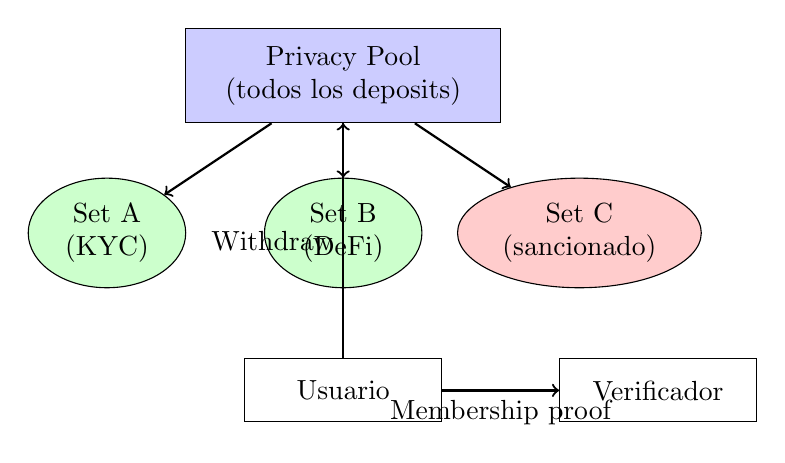
\begin{tikzpicture}[
    node distance=1cm,
    box/.style={draw, rectangle, minimum width=2.5cm, minimum height=0.8cm, align=center},
    set/.style={draw, ellipse, minimum width=2cm, minimum height=1cm, align=center},
    arrow/.style={->, thick}
]
    % Pool principal
    \node[box, fill=blue!20, minimum width=4cm, minimum height=1.2cm] (pool) at (4,3) {Privacy Pool\\(todos los deposits)};
    
    % Association Sets
    \node[set, fill=green!20] (good1) at (1,1) {Set A\\(KYC)};
    \node[set, fill=green!20] (good2) at (4,1) {Set B\\(DeFi)};
    \node[set, fill=red!20] (bad) at (7,1) {Set C\\(sancionado)};
    
    % Usuario
    \node[box] (user) at (4,-1) {Usuario};
    
    % Verificador
    \node[box] (verifier) at (8,-1) {Verificador};
    
    % Flechas
    \draw[arrow] (pool) -- (good1);
    \draw[arrow] (pool) -- (good2);
    \draw[arrow] (pool) -- (bad);
    
    \draw[arrow] (user) -- node[left] {Withdraw} (pool);
    \draw[arrow] (user) -- node[below] {Membership proof} (verifier);
\end{tikzpicture}
\end{center}

\subsection{Tipos de Association Sets}

\begin{definition}[Association Set Providers (ASPs)]
Entidades que definen y mantienen association sets:
\begin{itemize}
    \item \textbf{Exchanges:} Set de direcciones verificadas KYC
    \item \textbf{Chainalysis/Elliptic:} Sets de direcciones ``limpias'' o ``sucias''
    \item \textbf{DAOs:} Sets curados por la comunidad
    \item \textbf{Gobiernos:} Sets de direcciones sancionadas
\end{itemize}
\end{definition}

\begin{mathnote}
\textbf{Pruebas de Membership/Exclusion:}

\textbf{Membership Proof:}
\begin{itemize}
    \item Input p\'ublico: Ra\'iz del Merkle tree del Association Set
    \item Input privado: Tu nota, Merkle proof de inclusi\'on
    \item Output: ``Mi nota est\'a en este set''
\end{itemize}

\textbf{Exclusion Proof:}
\begin{itemize}
    \item Input p\'ublico: Ra\'iz del Merkle tree del Bad Set
    \item Input privado: Tu nota, prueba de no-inclusi\'on (m\'as compleja)
    \item Output: ``Mi nota NO est\'a en este set''
\end{itemize}

La prueba de no-inclusi\'on t\'ipicamente usa sparse Merkle trees o accumulators criptogr\'aficos.
\end{mathnote}

%===========================================
\section{zkML (Zero-Knowledge Machine Learning)}
\label{sec:zkml}
%===========================================

\subsection{Motivaci\'on}

\begin{definition}[zkML]
Aplicaci\'on de pruebas de conocimiento cero a modelos de machine learning, permitiendo:
\begin{itemize}
    \item Probar que un modelo produjo cierto output sin revelar el modelo
    \item Probar que un input produjo cierto output sin revelar el input
    \item Verificar que se us\'o un modelo espec\'ifico (modelo auditable)
\end{itemize}
\end{definition}

\begin{intuicion}
Imagina que tienes un modelo de ML para scoring crediticio. Quieres:
\begin{itemize}
    \item Demostrar al regulador que usas un modelo aprobado
    \item Sin revelar los par\'ametros exactos (propiedad intelectual)
    \item Sin revelar los datos del cliente (privacidad)
\end{itemize}

zkML permite esto: el regulador verifica una prueba de que ``el modelo aprobado dice que este cliente tiene score > 700'', sin ver el modelo ni los datos del cliente.
\end{intuicion}

\subsection{Casos de Uso de zkML}

\begin{enumerate}
    \item \textbf{On-chain AI:}
    \begin{itemize}
        \item Ejecutar inferencia ML off-chain
        \item Verificar resultado on-chain con ZK proof
        \item Ej: Or\'aculos de ML, NPCs en juegos, content moderation
    \end{itemize}
    
    \item \textbf{Private ML Inference:}
    \begin{itemize}
        \item Usuario tiene datos privados
        \item Proveedor tiene modelo privado
        \item Ambos verifican resultado sin revelar sus secretos
    \end{itemize}
    
    \item \textbf{Model Auditing:}
    \begin{itemize}
        \item Probar que el modelo no es discriminatorio
        \item Probar que se entren\'o con datos autorizados
        \item Sin revelar el modelo completo
    \end{itemize}
    
    \item \textbf{Proof-of-Personhood:}
    \begin{itemize}
        \item Probar que una imagen es de humano real
        \item Sin revelar la imagen
        \item \'Util contra bots y Sybil attacks
    \end{itemize}
\end{enumerate}

\subsection{Desaf\'ios T\'ecnicos}

\begin{remark}
\textbf{zkML es computacionalmente intensivo:}

\begin{itemize}
    \item \textbf{Modelos grandes = circuitos enormes:}
    \begin{itemize}
        \item GPT-2 small (124M params) $\to$ $\sim$100B constraints
        \item Inviable con tecnolog\'ia actual
    \end{itemize}
    
    \item \textbf{Operaciones no-ZK-friendly:}
    \begin{itemize}
        \item Division, sqrt, exp $\to$ costosos en circuitos
        \item Floating point $\to$ se usa fixed point
        \item Non-linear activations (ReLU, sigmoid) $\to$ aproximaciones
    \end{itemize}
    
    \item \textbf{Estado del arte:}
    \begin{itemize}
        \item Modelos peque\~nos ($<$1M params) son viables
        \item CNNs simples, decision trees, linear regression
        \item Tiempo de proof: minutos a horas
    \end{itemize}
\end{itemize}
\end{remark}

\subsection{Proyectos de zkML}

\begin{center}
\begin{tabular}{lcc}
\toprule
\textbf{Proyecto} & \textbf{Enfoque} & \textbf{Modelos Soportados} \\
\midrule
EZKL & PyTorch/ONNX $\to$ Halo2 & CNNs peque\~nos, transformers mini \\
Modulus Labs & Circuitos optimizados & Custom models \\
Giza & Cairo/StarkNet & ONNX models \\
Worldcoin & Iris recognition & Neural network espec\'ifico \\
Zkonduit & Halo2 backend & ONNX export \\
\bottomrule
\end{tabular}
\end{center}

\begin{bancozk}
\textbf{zkML en Banco ZK:}

Banco ZK explora zkML para varios casos de uso:

\begin{itemize}
    \item \textbf{Compliance autom\'atico:}
    \begin{itemize}
        \item Modelo de ML clasifica transacciones como suspicious/clean
        \item Usuario genera prueba de que su transacci\'on es ``clean'' seg\'un el modelo
        \item Sin revelar detalles de la transacci\'on
    \end{itemize}
    
    \item \textbf{Credit scoring privado:}
    \begin{itemize}
        \item Usuario tiene historial on-chain
        \item Modelo de credit scoring aprobado por regulador
        \item Usuario prueba ``mi score > threshold'' sin revelar score exacto ni historial
    \end{itemize}
    
    \item \textbf{Fraud detection:}
    \begin{itemize}
        \item Modelo detecta patrones de fraude
        \item Se verifica que todas las transacciones pasaron el modelo
        \item Sin revelar el modelo (evita gaming) ni las transacciones
    \end{itemize}
\end{itemize}

Nota: Esto es experimental y los modelos deben ser peque\~nos ($<$100K params) para ser pr\'acticos actualmente.
\end{bancozk}

%===========================================
\section{Resumen del Cap\'itulo}
\label{sec:resumen-cap4}
%===========================================

\begin{keyidea}
\textbf{Puntos clave de DeFi y Aplicaciones:}

\textbf{1. AMMs:}
\begin{itemize}
    \item Constant Product: $xy = k$, slippage proporcional al trade
    \item Concentrated Liquidity: Mayor eficiencia, mayor riesgo de IL
    \item StableSwap: Optimizado para stablecoins, bajo slippage
    \item IL inevitable, compensada por fees
\end{itemize}

\textbf{2. Lending:}
\begin{itemize}
    \item Tasas basadas en utilizaci\'on (modelo con ``kink'')
    \item Overcollateralized: siempre depositas m\'as de lo que pides
    \item Health Factor $< 1$ $\to$ liquidaci\'on
    \item Flash loans: pr\'estamos at\'omicos sin colateral
\end{itemize}

\textbf{3. Or\'aculos:}
\begin{itemize}
    \item Traen datos externos a blockchain
    \item TWAP > spot price (resistencia a manipulaci\'on)
    \item Siempre verificar freshness y sanity bounds
    \item Chainlink VRF para aleatoriedad verificable
\end{itemize}

\textbf{4. ZK Bridges:}
\begin{itemize}
    \item Verificaci\'on criptogr\'afica vs confianza en operadores
    \item Light clients ZK verifican consenso de otras cadenas
    \item M\'as seguro pero m\'as lento que bridges tradicionales
    \item Proyectos: Succinct, Lagrange, Polyhedra
\end{itemize}

\textbf{5. Atomic Swaps:}
\begin{itemize}
    \item HTLC: hashlock + timelock para intercambios trustless
    \item Tiempos largos y problema de ``free option''
    \item ZK Atomic Swaps permiten montos privados
\end{itemize}

\textbf{6. Cross-chain:}
\begin{itemize}
    \item IBC: Light clients nativos (Cosmos)
    \item LayerZero: Oracle + Relayer modular
    \item Axelar/Wormhole: Validadores/Guardians
\end{itemize}

\textbf{7. Privacy Pools:}
\begin{itemize}
    \item Balance entre privacidad y compliance
    \item Association Sets definen grupos ``buenos''/``malos''
    \item Membership proofs sin revelar transacci\'on espec\'ifica
\end{itemize}

\textbf{8. zkML:}
\begin{itemize}
    \item ML + ZK = inferencia verificable y/o privada
    \item Solo modelos peque\~nos son pr\'acticos actualmente
    \item Casos: on-chain AI, compliance, fraud detection
\end{itemize}
\end{keyidea}

\begin{bancozk}
\textbf{DeFi en Banco ZK --- Visi\'on General:}

Banco ZK integra DeFi con privacidad en todos los niveles:

\begin{center}
\begin{tabular}{lcc}
\toprule
\textbf{Componente} & \textbf{P\'ublico} & \textbf{Privado} \\
\midrule
AMM & Precios, liquidez total & Trades individuales \\
Lending & Tasas, utilizaci\'on & Posiciones de usuarios \\
Oracle & Precios de mercado & Verificaciones individuales \\
Bridge & Ra\'iz de estado & Transacciones espec\'ificas \\
Compliance & Sets aprobados & Membership individual \\
\bottomrule
\end{tabular}
\end{center}

Principio gu\'ia: \textit{``M\'axima privacidad para usuarios, m\'axima transparencia para el sistema.''}
\end{bancozk}

% ============================================
% FIN DEL CAP\'ITULO 4 (CAP 9 ORIGINAL)
% ============================================

% ============================================
% CAP\'ITULO 5: AVANZADO E INVESTIGACI\'ON
% (Cap 10 Original $\to$ Cap 5 Vol 2)
% ============================================

\chapter{Avanzado e Investigaci\'on}
\label{ch:avanzado-investigacion}

\section*{Introducci\'on}

Este cap\'itulo explora los temas m\'as avanzados y las fronteras de investigaci\'on en Zero-Knowledge Proofs. Desde la verificaci\'on formal que garantiza la correcci\'on de circuitos, hasta sistemas post-cu\'anticos que preparan la tecnolog\'ia para el futuro, estos temas representan el estado del arte y las direcciones futuras del campo.

\begin{keyidea}
Los temas de este cap\'itulo son relevantes para:
\begin{itemize}
    \item \textbf{Desarrolladores avanzados:} Optimizaci\'on y verificaci\'on formal
    \item \textbf{Arquitectos de sistemas:} Agregaci\'on y recursi\'on de pruebas
    \item \textbf{Investigadores:} Fronteras del conocimiento (zkML, post-quantum)
    \item \textbf{Planificadores:} Preparaci\'on para computaci\'on cu\'antica
\end{itemize}
\end{keyidea}

%===========================================
\section{zkML Avanzado}
\label{sec:zkml-advanced}
%===========================================

\subsection{Fundamentos y Arquitectura}

\begin{definition}[Zero-Knowledge Machine Learning]
zkML es la aplicaci\'on de pruebas de conocimiento cero a modelos de machine learning, permitiendo:
\begin{enumerate}
    \item \textbf{Inferencia verificable:} Probar que un modelo produjo cierto output
    \item \textbf{Inferencia privada:} Ejecutar ML sin revelar inputs o modelo
    \item \textbf{ML on-chain:} Verificar resultados de ML en blockchain
    \item \textbf{Auditor\'ia de modelos:} Probar propiedades del modelo sin revelarlo
\end{enumerate}
\end{definition}

\begin{mathnote}
\textbf{Timeline de zkML:}
\begin{itemize}
    \item \textbf{2020:} Primeros papers sobre ML verificable con ZK
    \item \textbf{2021:} EZKL comienza desarrollo (PyTorch $\to$ ZK)
    \item \textbf{2022:} Modulus Labs prueba concepto con modelos peque\~nos
    \item \textbf{2023:} Worldcoin usa zkML para verificaci\'on de iris
    \item \textbf{2023:} EZKL alcanza producci\'on, Giza en StarkNet
    \item \textbf{2024:} Mejoras en eficiencia, modelos m\'as grandes viables
    \item \textbf{2025+:} Investigaci\'on en transformers ZK-friendly
\end{itemize}
\end{mathnote}

\begin{intuicion}
\textbf{?`Por qu\'e zkML?}

Imagina que tienes un modelo de ML que detecta fraude financiero. Quieres:
\begin{itemize}
    \item Demostrar a un auditor que usaste el modelo aprobado
    \item Sin revelar los par\'ametros exactos (tu ventaja competitiva)
    \item Sin revelar los datos del cliente (privacidad, GDPR)
\end{itemize}

Con zkML, generas una prueba que dice: ``El modelo $M$ con hash $h_M$, aplicado al input con hash $h_x$, produjo output $y$''. El auditor puede verificar esto sin ver $M$ ni $x$.
\end{intuicion}

\begin{center}
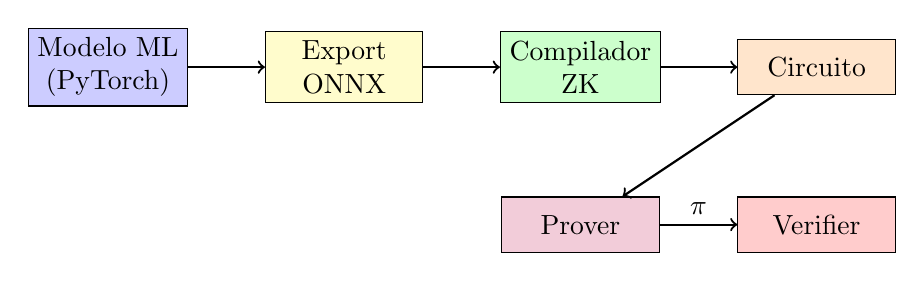
\begin{tikzpicture}[
    node distance=1cm,
    box/.style={draw, rectangle, minimum width=2cm, minimum height=0.7cm, align=center},
    arrow/.style={->, thick}
]
    % Pipeline
    \node[box, fill=blue!20] (model) at (0,0) {Modelo ML\\(PyTorch)};
    \node[box, fill=yellow!20] (export) at (3,0) {Export\\ONNX};
    \node[box, fill=green!20] (compile) at (6,0) {Compilador\\ZK};
    \node[box, fill=orange!20] (circuit) at (9,0) {Circuito};
    
    \node[box, fill=purple!20] (prove) at (6,-2) {Prover};
    \node[box, fill=red!20] (verify) at (9,-2) {Verifier};
    
    % Flechas
    \draw[arrow] (model) -- (export);
    \draw[arrow] (export) -- (compile);
    \draw[arrow] (compile) -- (circuit);
    \draw[arrow] (circuit) -- (prove);
    \draw[arrow] (prove) -- node[above] {$\pi$} (verify);
\end{tikzpicture}
\end{center}

\subsection{Desaf\'ios T\'ecnicos de zkML}

\subsubsection{Aritm\'etica de Punto Flotante}

\begin{remark}
\textbf{El Problema:} Los circuitos ZK operan sobre campos finitos $\mathbb{F}_p$, pero ML usa punto flotante IEEE 754.

No puedes hacer ``$3.14159 \times 2.71828$'' en un campo finito directamente.
\end{remark}

\begin{definition}[Fixed-Point Arithmetic]
Representaci\'on de n\'umeros reales usando enteros con punto decimal impl\'icito:
\[
x_{fixed} = \lfloor x_{float} \times 2^{scale} \rfloor
\]

Donde $scale$ es el n\'umero de bits fraccionales (t\'ipicamente 16-32).

\textbf{Operaciones:}
\begin{align}
(a + b)_{fixed} &= a_{fixed} + b_{fixed} \\
(a \times b)_{fixed} &= \frac{a_{fixed} \times b_{fixed}}{2^{scale}}
\end{align}
\end{definition}

\begin{mathnote}
\textbf{Error de Cuantizaci\'on:}

El error m\'aximo de fixed-point con $scale$ bits es:
\[
\epsilon_{max} = \frac{1}{2^{scale+1}}
\]

Para $scale = 16$: $\epsilon_{max} \approx 7.6 \times 10^{-6}$

Este error se \textbf{acumula} a trav\'es de las capas del modelo. Un modelo con 100 capas puede tener error acumulado significativo.
\end{mathnote}

\subsubsection{Funciones de Activaci\'on No Lineales}

\begin{remark}
Las funciones de activaci\'on comunes son \textbf{muy costosas} en circuitos:
\begin{itemize}
    \item \textbf{ReLU:} $\max(0, x)$ requiere comparaci\'on $\to$ bits de descomposici\'on
    \item \textbf{Sigmoid:} $\frac{1}{1+e^{-x}}$ requiere exponencial y divisi\'on
    \item \textbf{Softmax:} Exponenciales + divisi\'on + suma
    \item \textbf{GELU:} A\'un m\'as complejo (usado en transformers)
\end{itemize}
\end{remark}

\begin{definition}[Aproximaciones ZK-Friendly]
\textbf{ReLU:}
\begin{itemize}
    \item Descomponer $x$ en bits para determinar signo
    \item $\sim 254$ constraints para un n\'umero de 254 bits
    \item Optimizaci\'on: usar lookup tables
\end{itemize}

\textbf{Sigmoid (aproximaci\'on polinomial):}
\[
\sigma(x) \approx 0.5 + 0.25x - 0.0208x^3 \quad \text{para } x \in [-4, 4]
\]
\end{definition}

\subsubsection{Costo de Operaciones}

\begin{center}
\begin{tabular}{lcc}
\toprule
\textbf{Operaci\'on} & \textbf{Constraints (aprox)} & \textbf{Notas} \\
\midrule
Suma & 0 & Gratis (lineal) \\
Multiplicaci\'on & 1 & Operaci\'on base \\
Divisi\'on & $\sim$500 & Requiere inverse \\
ReLU (bit decomp) & $\sim$254 & Por cada activaci\'on \\
ReLU (lookup) & $\sim$3 & Con tabla pre-computada \\
Sigmoid (poly) & $\sim$5 & Aproximaci\'on c\'ubica \\
Matrix Mul $(n \times m) \times (m \times k)$ & $n \times m \times k$ & Dominante en redes \\
\bottomrule
\end{tabular}
\end{center}

\begin{example}[Costo de una Red Simple]
\textbf{Modelo:} MLP con arquitectura 784 $\to$ 128 $\to$ 64 $\to$ 10 (MNIST classifier)

\textbf{Capa 1:} $784 \times 128 = 100,352$ multiplicaciones + 128 ReLU

\textbf{Capa 2:} $128 \times 64 = 8,192$ multiplicaciones + 64 ReLU

\textbf{Capa 3:} $64 \times 10 = 640$ multiplicaciones

\textbf{Total (con ReLU lookup):}
\begin{itemize}
    \item Multiplicaciones: $100,352 + 8,192 + 640 = 109,184$ constraints
    \item ReLU: $(128 + 64) \times 3 = 576$ constraints (lookup)
    \item \textbf{Total:} $\sim$110,000 constraints
\end{itemize}

Tiempo de proving (Halo2, CPU): $\sim$30 segundos
\end{example}

\subsection{Frameworks de zkML}

\begin{definition}[EZKL]
Framework que compila modelos ONNX a circuitos Halo2:
\begin{itemize}
    \item \textbf{Input:} Modelo PyTorch/TensorFlow exportado a ONNX
    \item \textbf{Output:} Circuito Halo2 + prover + verifier Solidity
    \item \textbf{Features:} Calibraci\'on autom\'atica, lookups, optimizaciones
\end{itemize}
\end{definition}

\begin{definition}[Giza (StarkNet)]
Plataforma zkML para StarkNet usando STARKs:
\begin{itemize}
    \item \textbf{Ventaja:} STARKs son post-quantum
    \item \textbf{Proceso:} ONNX $\to$ Cairo $\to$ STARK proof
    \item \textbf{Verificaci\'on:} Nativa en StarkNet
\end{itemize}
\end{definition}

\subsection{Aplicaciones Pr\'acticas de zkML}

\subsubsection{Proof of Personhood (Worldcoin)}

\begin{definition}[Worldcoin Iris Verification]
Sistema que prueba unicidad de persona usando escaneo de iris:
\begin{enumerate}
    \item \textbf{Captura:} Orb escanea iris del usuario
    \item \textbf{Modelo ML:} Extrae embedding del iris
    \item \textbf{ZK Proof:} Prueba que embedding es \'unico sin revelarlo
    \item \textbf{On-chain:} Verifica prueba y registra identidad
\end{enumerate}
\end{definition}

\subsubsection{Private Credit Scoring}

\begin{example}[Credit Scoring Privado]
Un circuito que prueba ``Mi score es $\geq$ threshold'' sin revelar el score exacto:
\begin{verbatim}
template PrivateCreditScore(nFeatures) {
    signal input features[nFeatures];     // Datos financieros (privados)
    signal input modelCommitment;         // Hash de los pesos (p\'ublico)
    signal input threshold;               // Score m\'inimo requerido
    signal output meetsThreshold;         // 1 si score >= threshold
    
    // Ejecutar modelo y comparar con threshold
    // Solo revela: ''cumple'' o ''no cumple''
}
\end{verbatim}
\end{example}

\subsection{Limitaciones Actuales}

\begin{remark}
\textbf{Limitaciones de zkML (2025):}

\begin{enumerate}
    \item \textbf{Tama\~no de modelos:}
    \begin{itemize}
        \item Viable: $<$ 1M par\'ametros
        \item Posible con optimizaci\'on: 1-10M par\'ametros
        \item Imposible hoy: GPT-2 (124M), BERT (110M), LLaMA (7B+)
    \end{itemize}
    
    \item \textbf{Tiempo de proving:}
    \begin{itemize}
        \item Modelo peque\~no: segundos a minutos
        \item Modelo mediano: minutos a horas
        \item No es real-time para la mayor\'ia de casos
    \end{itemize}
    
    \item \textbf{Precisi\'on:}
    \begin{itemize}
        \item Fixed-point introduce error de cuantizaci\'on
        \item Aproximaciones de activaciones reducen accuracy
        \item T\'ipicamente 1-5\% p\'erdida de accuracy vs float32
    \end{itemize}
\end{enumerate}
\end{remark}

\begin{keyidea}
\textbf{Direcciones de investigaci\'on para zkML:}
\begin{enumerate}
    \item \textbf{Modelos ZK-native:} Entrenar modelos optimizados para ZK desde el inicio
    \item \textbf{Pruning y quantization:} Reducir tama\~no del modelo manteniendo accuracy
    \item \textbf{Hardware acceleration:} GPUs y ASICs para proving de ML
    \item \textbf{Folding para ML:} Aplicar t\'ecnicas de folding (Nova) a capas
\end{enumerate}
\end{keyidea}

%===========================================
\section{Verificaci\'on Formal de Circuitos}
\label{sec:formal-verification}
%===========================================

\subsection{Motivaci\'on: El Problema de Soundness}

\begin{definition}[Soundness en Circuitos ZK]
Un circuito es \textbf{sound} si solo acepta witnesses v\'alidos. Un circuito \textbf{unsound} acepta witnesses que no deber\'ian ser v\'alidos, permitiendo generar pruebas falsas.
\end{definition}

\begin{remark}
\textbf{Bugs de soundness son catastr\'oficos:}

Si un circuito tiene un bug que permite crear pruebas falsas, un atacante puede:
\begin{itemize}
    \item Generar dinero de la nada en un L2
    \item Probar transacciones que nunca ocurrieron
    \item Bypassear toda la seguridad del sistema
\end{itemize}

A diferencia de bugs en smart contracts (donde al menos el estado es visible), bugs en circuitos ZK pueden ser explotados \textbf{sin dejar rastro}.
\end{remark}

\begin{mathnote}
\textbf{Historial de Bugs en Circuitos:}
\begin{itemize}
    \item \textbf{Zcash (2019):} Bug de inflaci\'on potencial en circuito Sprout
    \item \textbf{Tornado Cash (2022):} Under-constraint permit\'ia doble gasto
    \item \textbf{Circom bugs varios:} M\'ultiples under-constraints en circomlib
    \item \textbf{zkSync (2023):} Bug en verificador que fue parcheado
\end{itemize}
\end{mathnote}

\subsection{Tipos de Bugs en Circuitos}

\begin{definition}[Under-Constrained Circuit]
Un circuito est\'a \textbf{under-constrained} cuando existen m\'ultiples witnesses v\'alidos para el mismo set de inputs p\'ublicos, pero solo algunos representan computaciones leg\'itimas.

\textbf{Ejemplo:}
\begin{verbatim}
// Bug: under-constrained
template BadSquare() {
    signal input x;
    signal output y;
    
    y <-- x * x;  // Solo asigna, no constra\~na
    // Falta: y === x * x;
}
\end{verbatim}

En este caso, el prover puede asignar cualquier valor a $y$, no necesariamente $x^2$.
\end{definition}

\begin{definition}[Over-Constrained Circuit]
Un circuito est\'a \textbf{over-constrained} cuando rechaza witnesses v\'alidos, o es directamente insatisfacible.
\end{definition}

\begin{definition}[Constraint Confusion]
Confusi\'on entre asignaci\'on (\texttt{<--}) y constraint (\texttt{===}):

\begin{verbatim}
// CORRECTO
y <== x * x;  // Asigna Y constra\~na

// INCORRECTO (bug com\'un)
y <-- x * x;  // Solo asigna, NO constra\~na
\end{verbatim}
\end{definition}

\subsection{Verificaci\'on Formal: Conceptos}

\begin{definition}[Verificaci\'on Formal]
Proceso de probar matem\'aticamente que un circuito satisface su especificaci\'on usando:
\begin{itemize}
    \item \textbf{Model checking:} Exploraci\'on exhaustiva del espacio de estados
    \item \textbf{Theorem proving:} Demostraci\'on matem\'atica de propiedades
    \item \textbf{SMT solving:} Satisfiability Modulo Theories
\end{itemize}
\end{definition}

\begin{intuicion}
Testing prueba que ``para estos inputs, el circuito funciona''.

Verificaci\'on formal prueba que ``para TODOS los inputs posibles, el circuito funciona''.

Es la diferencia entre probar 1 mill\'on de casos vs probar infinitos casos.
\end{intuicion}

\subsubsection{Propiedades a Verificar}

\begin{definition}[Propiedades de Correctness]
\begin{enumerate}
    \item \textbf{Completeness:} Para todo input v\'alido, existe un witness que satisface el circuito
    \[
    \forall x \in \text{Valid}: \exists w: C(x, w) = 1
    \]
    
    \item \textbf{Soundness:} Solo inputs v\'alidos tienen witnesses que satisfacen el circuito
    \[
    \forall x, w: C(x, w) = 1 \implies x \in \text{Valid}
    \]
    
    \item \textbf{Determinism:} Para cada input p\'ublico, hay exactamente un output v\'alido
\end{enumerate}
\end{definition}

\subsection{Herramientas de Verificaci\'on Formal}

\begin{definition}[Ecne]
Verificador formal para circuitos R1CS:
\begin{itemize}
    \item \textbf{Input:} Circuito R1CS + especificaci\'on
    \item \textbf{M\'etodo:} SMT solving (Z3, CVC5)
    \item \textbf{Output:} Prueba de correctness o contraejemplo
\end{itemize}
\end{definition}

\begin{definition}[Picus]
Verificador que detecta under-constraints autom\'aticamente:
\begin{itemize}
    \item \textbf{An\'alisis est\'atico:} Sin ejecutar el circuito
    \item \textbf{Detecci\'on de under-constraints:} Se\~nales que pueden tomar m\'ultiples valores
    \item \textbf{Visualizaci\'on:} Muestra qu\'e se\~nales son problem\'aticas
\end{itemize}
\end{definition}

\begin{definition}[Circomspect]
Linter y analizador est\'atico para Circom:
\begin{itemize}
    \item \textbf{Detecci\'on de patrones:} Anti-patterns comunes
    \item \textbf{Under-constraint detection:} Se\~nales sin suficientes constraints
    \item \textbf{Side-effect analysis:} Asignaciones sin constraints correspondientes
\end{itemize}
\end{definition}

\subsection{Best Practices para Circuitos Seguros}

\begin{keyidea}
\textbf{Reglas de oro para circuitos seguros:}

\begin{enumerate}
    \item \textbf{Siempre usar \texttt{<==} en lugar de \texttt{<--}}
    \begin{itemize}
        \item \texttt{<--} es solo para casos especiales donde el constraint viene despu\'es
        \item Cuando uses \texttt{<--}, documenta POR QU\'E y d\'onde est\'a el constraint
    \end{itemize}
    
    \item \textbf{Constra\~nir todos los inputs a sus rangos v\'alidos}
    \begin{verbatim}
// Malo: bit no constrained
signal input bit;
out <== x + bit * y;

// Bueno: verificar que es 0 o 1
signal input bit;
bit * (1 - bit) === 0;
out <== x + bit * y;
    \end{verbatim}
    
    \item \textbf{Nunca confiar en el prover}
    \begin{itemize}
        \item El prover es potencialmente malicioso
        \item Toda se\~nal que afecte el resultado debe ser constrained
    \end{itemize}
    
    \item \textbf{Usar templates auditados}
    \begin{itemize}
        \item circomlib tiene bugs hist\'oricos --- usar versiones actualizadas
        \item Preferir templates ampliamente usados y auditados
    \end{itemize}
    
    \item \textbf{Testing no es suficiente}
    \begin{itemize}
        \item Un test pasa con witness honesto
        \item Un atacante usa witness deshonesto
        \item Verificaci\'on formal detecta lo que testing no puede
    \end{itemize}
\end{enumerate}
\end{keyidea}

%===========================================
\section{Optimizaci\'on de Circuitos}
\label{sec:circuit-optimization}
%===========================================

\subsection{M\'etricas de Eficiencia}

\begin{definition}[M\'etricas de Circuitos]
\begin{itemize}
    \item \textbf{N\'umero de constraints:} Principal m\'etrica para R1CS/Plonk
    \item \textbf{N\'umero de multiplicaciones:} Solo multiplicaciones cuestan constraints
    \item \textbf{Profundidad del circuito:} Afecta paralelizaci\'on
    \item \textbf{N\'umero de se\~nales:} Afecta memoria del prover
    \item \textbf{Tiempo de proving:} M\'etrica final
\end{itemize}
\end{definition}

\begin{mathnote}
\textbf{Complejidad de Proving:}

Para un circuito con $n$ constraints:
\begin{itemize}
    \item \textbf{Groth16:} Proving $O(n \log n)$, Verificaci\'on $O(1)$
    \item \textbf{PLONK:} Proving $O(n \log n)$, Verificaci\'on $O(\log n)$
    \item \textbf{STARKs:} Proving $O(n \log^2 n)$, Verificaci\'on $O(\log^2 n)$
\end{itemize}

Reducir $n$ a la mitad aproximadamente reduce tiempo de proving a la mitad.
\end{mathnote}

\subsection{T\'ecnicas de Optimizaci\'on}

\subsubsection{Reducci\'on de Multiplicaciones}

\begin{keyidea}
En R1CS, solo las multiplicaciones generan constraints. Las sumas son ``gratis''.

\textbf{R1CS:} $A \cdot B = C$ donde $A$, $B$, $C$ son combinaciones lineales.

Si puedes reescribir tu computaci\'on usando menos multiplicaciones, reduces constraints.
\end{keyidea}

\begin{example}[Optimizaci\'on de Polinomio]
Calcular $y = x^3 + 2x^2 + 3x + 4$

\textbf{M\'etodo naive (3 multiplicaciones):}
\begin{verbatim}
x2 <== x * x;       // Mult 1
x3 <== x2 * x;      // Mult 2
y <== x3 + 2*x2 + 3*x + 4;  // Sin mult
\end{verbatim}

\textbf{M\'etodo Horner (2 multiplicaciones):}
\[
y = ((x + 2) \cdot x + 3) \cdot x + 4
\]
\begin{verbatim}
t1 <== (x + 2) * x;      // Mult 1
t2 <== (t1 + 3) * x;     // Mult 2
y <== t2 + 4;            // Sin mult
\end{verbatim}

\textbf{Ahorro:} 33\% menos constraints
\end{example}

\subsubsection{Lookup Arguments}

\begin{definition}[Lookup Argument]
T\'ecnica que permite verificar que un valor pertenece a una tabla predefinida con costo constante (o logar\'itmico), en lugar de calcularlo expl\'icitamente.
\end{definition}

\begin{intuicion}
En lugar de calcular $y = \sqrt{x}$ en el circuito (muy costoso), pre-computas una tabla con todos los valores posibles de $x$ y $\sqrt{x}$.

Luego el circuito solo verifica: ``$(x, y)$ est\'a en la tabla''.

Es como buscar en un diccionario vs derivar la definici\'on desde primeros principios.
\end{intuicion}

\begin{example}[ReLU con Lookup]
\textbf{Sin lookup (254 constraints para ReLU):}

Necesitas descomponer en bits para determinar signo.

\textbf{Con lookup (3-5 constraints):}

El circuito solo verifica membership en la tabla ReLU.

\textbf{Ahorro:} 50-100x menos constraints para operaciones no-lineales
\end{example}

\begin{mathnote}
\textbf{Plookup:}

Plookup es el lookup argument m\'as usado:
\begin{itemize}
    \item \textbf{Setup:} Tabla $T$ de tama\~no $|T|$
    \item \textbf{Proving:} $O(|T| \log |T|)$ para $n$ lookups
    \item \textbf{Constraint overhead:} $\sim$3 constraints por lookup
    \item \textbf{Limitaci\'on:} Tabla debe ser conocida en compile time
\end{itemize}

Ideal para: XOR, AND, range checks, funciones no-lineales con dominio finito
\end{mathnote}

\subsubsection{Custom Gates (PLONKish)}

\begin{definition}[Custom Gate]
En sistemas PLONKish (PLONK, Halo2), puedes definir constraints personalizados m\'as all\'a de la multiplicaci\'on simple:
\[
q_L \cdot a + q_R \cdot b + q_O \cdot c + q_M \cdot ab + q_C = 0
\]

Los $q_i$ son ``selectores'' que activan/desactivan partes del gate.
\end{definition}

\begin{example}[Custom Gate para Poseidon]
Poseidon hash usa la operaci\'on $x^5$ (quintic) frecuentemente.

\textbf{Con gates est\'andar:} 3 gates, 3 rows

\textbf{Con custom gate para $x^5$:} 1 gate, 1 row

\textbf{Ahorro:} 66\% menos rows para cada $x^5$
\end{example}

\subsubsection{Selecci\'on de Campo}

\begin{definition}[Campo \'Optimo]
El campo finito $\mathbb{F}_p$ afecta la eficiencia:
\begin{itemize}
    \item \textbf{Tama\~no de $p$:} Campos m\'as peque\~nos = aritm\'etica m\'as r\'apida
    \item \textbf{Estructura de $p$:} $p = 2^k - c$ (Mersenne-like) es m\'as eficiente
    \item \textbf{Compatibilidad:} Debe ser compatible con curvas el\'ipticas usadas
\end{itemize}
\end{definition}

\begin{center}
\begin{tabular}{lccc}
\toprule
\textbf{Campo} & \textbf{Bits} & \textbf{Estructura} & \textbf{Uso} \\
\midrule
BN254 scalar & 254 & Gen\'erico & Ethereum, Groth16 \\
BLS12-381 scalar & 255 & Gen\'erico & Zcash, many SNARKs \\
Pasta (Pallas/Vesta) & 255 & Gen\'erico & Halo2, 2-cycles \\
Goldilocks & 64 & $2^{64} - 2^{32} + 1$ & Plonky2 (muy r\'apido) \\
BabyBear & 31 & $2^{31} - 2^{27} + 1$ & Risc Zero \\
M31 (Mersenne31) & 31 & $2^{31} - 1$ & STARKs, Circle \\
\bottomrule
\end{tabular}
\end{center}

\begin{keyidea}
\textbf{Trend actual:} Campos m\'as peque\~nos (64 bits o menos) son mucho m\'as r\'apidos.

Plonky2/Plonky3 usan Goldilocks (64 bits) y son $\sim$100x m\'as r\'apidos que sistemas sobre BN254.

Trade-off: Campos peque\~nos tienen menor seguridad contra ataques algebraicos, requieren m\'as rondas/repeticiones.
\end{keyidea}

\subsection{Hardware Acceleration}

\begin{definition}[Aceleraci\'on por Hardware]
\begin{itemize}
    \item \textbf{GPU:} 10-100x speedup para MSM y FFT
    \item \textbf{FPGA:} Custom circuits para operaciones espec\'ificas
    \item \textbf{ASIC:} M\'axima eficiencia, menor flexibilidad
\end{itemize}
\end{definition}

Benchmarks t\'ipicos ($2^{20}$ puntos MSM):
\begin{itemize}
    \item CPU (Ryzen 9): $\sim$15 segundos
    \item GPU (RTX 3090): $\sim$0.3 segundos
    \item Speedup: $\sim$50x
\end{itemize}

%===========================================
\section{Proof Aggregation}
\label{sec:proof-aggregation}
%===========================================

\subsection{Motivaci\'on}

\begin{definition}[Proof Aggregation]
T\'ecnica para combinar m\'ultiples pruebas ZK en una sola prueba m\'as peque\~na, reduciendo el costo de verificaci\'on.
\end{definition}

\begin{intuicion}
Imagina que tienes 1000 pruebas, cada una cuesta \$0.50 verificar on-chain.
Costo total: \$500.

Con agregaci\'on, combinas las 1000 pruebas en una sola.
Costo total: \$0.50 (m\'as el costo de agregar off-chain).

Es como enviar un cami\'on lleno de paquetes en lugar de 1000 entregas individuales.
\end{intuicion}

\begin{keyidea}
\textbf{Beneficios de la agregaci\'on:}
\begin{itemize}
    \item \textbf{Costo:} Verificaci\'on on-chain es costosa. Agregar reduce verificaciones.
    \item \textbf{Throughput:} Un rollup puede procesar m\'as transacciones por batch.
    \item \textbf{Latencia:} Menor data on-chain = confirmaci\'on m\'as r\'apida.
\end{itemize}

\textbf{Trade-off:}
\begin{itemize}
    \item Agregar tiene costo computacional off-chain
    \item Latencia de esperar por batch
    \item Complejidad del sistema
\end{itemize}
\end{keyidea}

\subsection{M\'etodos de Agregaci\'on}

\subsubsection{Recursive Proof Composition}

\begin{definition}[Recursive Proof]
Una prueba que verifica otra prueba dentro de su circuito:
\[
\pi_{outer} = \text{Prove}(\text{``}V(\pi_{inner}) = 1\text{''})
\]

El verificador del sistema interno se ``embebe'' en el circuito del sistema externo.
\end{definition}

\begin{center}
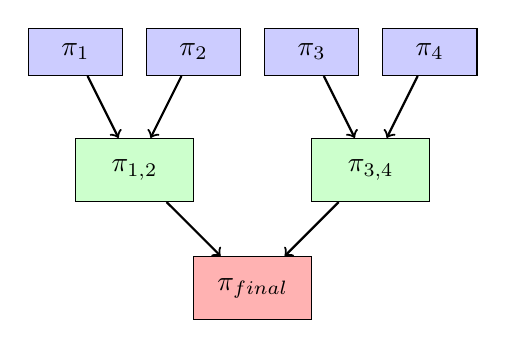
\begin{tikzpicture}[
    node distance=0.8cm,
    proof/.style={draw, rectangle, minimum width=1.2cm, minimum height=0.6cm, align=center, fill=blue!20},
    aggproof/.style={draw, rectangle, minimum width=1.5cm, minimum height=0.8cm, align=center, fill=green!20},
    arrow/.style={->, thick}
]
    % Nivel 1: Pruebas individuales
    \node[proof] (p1) at (0,0) {$\pi_1$};
    \node[proof] (p2) at (1.5,0) {$\pi_2$};
    \node[proof] (p3) at (3,0) {$\pi_3$};
    \node[proof] (p4) at (4.5,0) {$\pi_4$};
    
    % Nivel 2
    \node[aggproof] (a1) at (0.75,-1.5) {$\pi_{1,2}$};
    \node[aggproof] (a2) at (3.75,-1.5) {$\pi_{3,4}$};
    
    % Nivel 3
    \node[aggproof, fill=red!30] (final) at (2.25,-3) {$\pi_{final}$};
    
    % Flechas
    \draw[arrow] (p1) -- (a1);
    \draw[arrow] (p2) -- (a1);
    \draw[arrow] (p3) -- (a2);
    \draw[arrow] (p4) -- (a2);
    \draw[arrow] (a1) -- (final);
    \draw[arrow] (a2) -- (final);
\end{tikzpicture}
\end{center}

\begin{mathnote}
\textbf{Complejidad de Agregaci\'on Recursiva:}

Para $n$ pruebas con \'arbol binario:
\begin{itemize}
    \item N\'umero de niveles: $\lceil \log_2 n \rceil$
    \item N\'umero total de agregaciones: $n - 1$
    \item Tama\~no final: constante (independiente de $n$)
    \item Tiempo de agregaci\'on: $O(n)$ trabajo total
\end{itemize}
\end{mathnote}

\subsubsection{Batching (sin recursi\'on)}

\begin{definition}[Proof Batching]
Probar m\'ultiples statements en un solo circuito, sin verificar pruebas existentes:
\[
\pi_{batch} = \text{Prove}(x_1 \in L \land x_2 \in L \land ... \land x_n \in L)
\]
\end{definition}

\subsubsection{SnarkPack}

\begin{definition}[SnarkPack]
Esquema de agregaci\'on para Groth16:
\begin{itemize}
    \item Agrega $n$ pruebas Groth16 en una sola
    \item Tama\~no de prueba agregada: $O(\log n)$
    \item Verificaci\'on: $O(\log n)$
    \item No requiere recursi\'on (m\'as eficiente)
\end{itemize}
\end{definition}

%===========================================
\section{Sistemas Recursivos}
\label{sec:recursive-systems}
%===========================================

\subsection{Incrementally Verifiable Computation (IVC)}

\begin{definition}[IVC]
Sistema donde una computaci\'on de $n$ pasos se puede verificar incrementalmente:
\begin{itemize}
    \item Paso $i$: Prover genera $\pi_i$ que prueba ``los pasos $1..i$ son correctos''
    \item Paso $i+1$: Usando $\pi_i$, genera $\pi_{i+1}$ con costo independiente de $i$
\end{itemize}

La verificaci\'on final solo necesita $\pi_n$, sin importar cu\'an grande sea $n$.
\end{definition}

\begin{intuicion}
Imagina una cadena de c\'alculos: $s_0 \to s_1 \to s_2 \to ... \to s_n$

Sin IVC: Verificar requiere re-ejecutar todos los pasos.
Con IVC: La prueba final dice ``conf\'ia que $s_n$ es correcto'', y verificarla es $O(1)$.

Es como un sello de calidad que se va pasando y acumulando confianza.
\end{intuicion}

\begin{center}
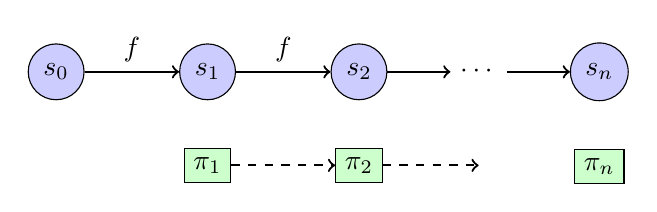
\begin{tikzpicture}[
    node distance=0.8cm,
    state/.style={draw, circle, minimum size=0.7cm, fill=blue!20},
    proof/.style={draw, rectangle, minimum width=0.5cm, minimum height=0.3cm, fill=green!20},
    arrow/.style={->, thick}
]
    % Estados
    \node[state] (s0) {$s_0$};
    \node[state, right=1.2cm of s0] (s1) {$s_1$};
    \node[state, right=1.2cm of s1] (s2) {$s_2$};
    \node[right=0.8cm of s2] (dots) {$\cdots$};
    \node[state, right=0.8cm of dots] (sn) {$s_n$};
    
    % Transiciones
    \draw[arrow] (s0) -- node[above] {$f$} (s1);
    \draw[arrow] (s1) -- node[above] {$f$} (s2);
    \draw[arrow] (s2) -- (dots);
    \draw[arrow] (dots) -- (sn);
    
    % Pruebas
    \node[proof, below=0.6cm of s1] (p1) {$\pi_1$};
    \node[proof, below=0.6cm of s2] (p2) {$\pi_2$};
    \node[proof, below=0.6cm of sn] (pn) {$\pi_n$};
    
    % Flechas de pruebas
    \draw[arrow, dashed] (p1) -- (p2);
    \draw[arrow, dashed] (p2) -- (dots |- p2);
\end{tikzpicture}
\end{center}

\subsection{Proof-Carrying Data (PCD)}

\begin{definition}[PCD]
Generalizaci\'on de IVC a grafos de computaci\'on (no solo cadenas):
\begin{itemize}
    \item M\'ultiples ``hilos'' de computaci\'on
    \item Pueden unirse (merge) y dividirse (fork)
    \item Cada nodo verifica las pruebas de sus predecesores
\end{itemize}
\end{definition}

\subsection{Aplicaciones de IVC/PCD}

\subsubsection{Blockchains Sucintas (Mina Protocol)}

\begin{definition}[Mina Protocol]
Blockchain donde el estado completo es una sola prueba ZK:
\begin{itemize}
    \item Cada bloque genera prueba IVC: ``los bloques $0..n$ son v\'alidos''
    \item Sincronizar = descargar una prueba de $\sim$22KB
    \item No necesitas descargar toda la historia
\end{itemize}
\end{definition}

\subsection{Folding Schemes}

\begin{definition}[Folding]
T\'ecnica para ``combinar'' dos instancias de un problema en una sola, sin generar una prueba completa:
\[
\text{Fold}(\text{instance}_1, \text{instance}_2) \to \text{instance}_{combined}
\]

M\'as eficiente que recursi\'on completa porque evita la verificaci\'on completa en cada paso.
\end{definition}

\begin{intuicion}
Recursi\'on tradicional: En cada paso, generas una prueba completa que verifica la prueba anterior. Esto es costoso.

Folding: En cada paso, solo ``combinas'' las instancias. Al final, generas UNA prueba de la instancia combinada.

Es como acumular trabajo pendiente y hacerlo todo al final, en lugar de completar cada tarea individualmente.
\end{intuicion}

\subsubsection{Nova}

\begin{definition}[Nova]
Esquema de folding para R1CS:
\begin{itemize}
    \item Fold: $O(n)$ operaciones de campo (sin FFT, sin MSM)
    \item Final proof: Una prueba Groth16/Spartan al final
    \item Muy eficiente para IVC
\end{itemize}
\end{definition}

\begin{mathnote}
\textbf{C\'omo funciona Nova:}

R1CS: $Az \circ Bz = Cz$

\textbf{Relaxed R1CS:} $Az \circ Bz = u \cdot Cz + E$

Donde:
\begin{itemize}
    \item $u$ es un escalar (``relaxation factor'')
    \item $E$ es un ``error vector''
\end{itemize}

\textbf{Folding:}
Dadas dos instancias $(u_1, E_1, z_1)$ y $(u_2, E_2, z_2)$:
\[
u' = u_1 + r \cdot u_2, \quad E' = E_1 + r \cdot T + r^2 \cdot E_2, \quad z' = z_1 + r \cdot z_2
\]

Donde $r$ es un challenge aleatorio y $T$ es un ``cross-term''.
\end{mathnote}

\subsubsection{SuperNova y HyperNova}

\begin{definition}[SuperNova]
Extensi\'on de Nova para circuitos con m\'ultiples ``opcodes'':
\begin{itemize}
    \item Cada paso puede ejecutar uno de $k$ circuitos diferentes
    \item Ideal para zkVMs (cada instrucci\'on es un circuito)
    \item Solo paga por el circuito m\'as grande, no la suma
\end{itemize}
\end{definition}

\begin{definition}[HyperNova]
Generalizaci\'on de Nova a CCS (Customizable Constraint Systems):
\begin{itemize}
    \item Soporta Plonkish, AIR, R1CS
    \item Folding m\'as general
    \item Puede ser m\'as eficiente para algunos circuitos
\end{itemize}
\end{definition}

\begin{center}
\begin{tabular}{lccc}
\toprule
\textbf{Esquema} & \textbf{Sistema Base} & \textbf{Costo por Fold} & \textbf{Aplicaci\'on} \\
\midrule
Nova & R1CS & $O(n)$ & IVC general \\
SuperNova & R1CS (multi) & $O(n)$ & zkVMs \\
HyperNova & CCS & $O(n)$ & Plonkish IVC \\
Sangria & Plonk & $O(n \log n)$ & Plonk native \\
\bottomrule
\end{tabular}
\end{center}

%===========================================
\section{Post-Quantum ZK}
\label{sec:post-quantum}
%===========================================

\subsection{La Amenaza Cu\'antica}

\begin{definition}[Computaci\'on Cu\'antica y Criptograf\'ia]
Las computadoras cu\'anticas pueden ejecutar algoritmos que rompen la seguridad de muchos sistemas criptogr\'aficos actuales:
\begin{itemize}
    \item \textbf{Algoritmo de Shor:} Factoriza enteros y calcula logaritmos discretos en tiempo polinomial
    \item \textbf{Algoritmo de Grover:} B\'usqueda en $O(\sqrt{N})$ en lugar de $O(N)$
\end{itemize}
\end{definition}

\begin{remark}
\textbf{Impacto en sistemas ZK actuales:}

\begin{itemize}
    \item \textbf{Groth16, PLONK (con KZG):} Basados en curvas el\'ipticas y pairings
    \begin{itemize}
        \item Shor rompe el problema del logaritmo discreto
        \item \textcolor{red}{Completamente inseguros ante computadoras cu\'anticas}
    \end{itemize}
    
    \item \textbf{Bulletproofs:} Basados en logaritmo discreto
    \begin{itemize}
        \item \textcolor{red}{Completamente inseguros ante computadoras cu\'anticas}
    \end{itemize}
    
    \item \textbf{STARKs:} Basados solo en funciones hash
    \begin{itemize}
        \item Grover reduce seguridad a la mitad (256-bit $\to$ 128-bit efectivo)
        \item \textcolor{green!50!black}{Seguro con par\'ametros adecuados}
    \end{itemize}
\end{itemize}
\end{remark}

\begin{mathnote}
\textbf{Timeline Estimado de Amenaza Cu\'antica:}
\begin{itemize}
    \item \textbf{2024:} Computadoras cu\'anticas con $\sim$1,000 qubits (ruidosos)
    \item \textbf{2030:} Posibles $\sim$10,000+ qubits con correcci\'on de errores
    \item \textbf{2035-2040:} Potencialmente capaces de romper RSA-2048 / ECDSA
\end{itemize}

Incertidumbre alta, pero el consenso es prepararse \textbf{ahora}:
\begin{itemize}
    \item ``Harvest now, decrypt later'' --- Adversarios pueden guardar datos cifrados
    \item Migraci\'on de sistemas toma a\~nos
    \item NIST ya estandariz\'o algoritmos post-cu\'anticos (2024)
\end{itemize}
\end{mathnote}

\subsection{An\'alisis de Seguridad por Sistema}

\begin{center}
\begin{tabular}{lcccl}
\toprule
\textbf{Sistema} & \textbf{Base Cripto} & \textbf{Post-Q} & \textbf{Proof Size} & \textbf{Notas} \\
\midrule
Groth16 & Pairings (EC) & \textcolor{red}{No} & 128 bytes & M\'as compacto \\
PLONK + KZG & Pairings (EC) & \textcolor{red}{No} & 400-800 bytes & Universal \\
PLONK + IPA & Log discreto & \textcolor{red}{No} & 1-2 KB & Sin trusted setup \\
Bulletproofs & Log discreto & \textcolor{red}{No} & 0.7-1.5 KB & Range proofs \\
\midrule
STARKs & Hash functions & \textcolor{green!50!black}{S\'i} & 50-200 KB & Transparente \\
FRI-based & Hash + Reed-Solomon & \textcolor{green!50!black}{S\'i} & 50-200 KB & Plonky2/3 \\
Lattice SNARKs & Lattices (LWE) & \textcolor{green!50!black}{S\'i} & 10-50 KB & En desarrollo \\
\bottomrule
\end{tabular}
\end{center}

\subsection{STARKs: La Opci\'on Post-Quantum Actual}

\begin{definition}[STARK Security]
La seguridad de STARKs se basa \'unicamente en:
\begin{enumerate}
    \item \textbf{Collision resistance de hash:} Dif\'icil encontrar $x \neq y$ con $H(x) = H(y)$
    \item \textbf{Random oracle model:} Hash se comporta como funci\'on aleatoria
\end{enumerate}

No depende de logaritmo discreto, factorizaci\'on, ni pairings.
\end{definition}

\begin{mathnote}
\textbf{Impacto de Grover en STARKs:}

Grover reduce la seguridad de b\'usqueda/colisi\'on:
\begin{itemize}
    \item Cl\'asico: Encontrar colisi\'on en hash de $n$ bits requiere $O(2^{n/2})$
    \item Cu\'antico (Grover): Requiere $O(2^{n/3})$ (para colisiones)
\end{itemize}

Para mantener 128 bits de seguridad post-cu\'antica:
\begin{itemize}
    \item Usar hash de al menos 256 bits
    \item STARKs t\'ipicamente usan 256+ bits de seguridad
    \item Pruebas m\'as grandes, pero seguras
\end{itemize}
\end{mathnote}

\subsection{Lattice-Based SNARKs}

\begin{definition}[Lattice Problems]
Problemas computacionales en lattices (ret\'iculas) que se creen resistentes a ataques cu\'anticos:
\begin{itemize}
    \item \textbf{LWE (Learning With Errors):} Distinguir $As + e$ de aleatorio
    \item \textbf{SIS (Short Integer Solution):} Encontrar vector corto $x$ con $Ax = 0$
    \item \textbf{Ring-LWE:} Versi\'on estructurada de LWE (m\'as eficiente)
\end{itemize}
\end{definition}

\begin{mathnote}
\textbf{Por qu\'e Lattices son Post-Quantum:}
\begin{itemize}
    \item No hay algoritmo cu\'antico conocido que resuelva LWE/SIS eficientemente
    \item Los mejores ataques (cl\'asicos y cu\'anticos) son exponenciales
    \item Base de los est\'andares NIST post-cu\'anticos (Kyber, Dilithium)
\end{itemize}
\end{mathnote}

\begin{remark}
\textbf{Limitaciones actuales de Lattice SNARKs:}
\begin{itemize}
    \item Pruebas m\'as grandes que SNARKs basados en curvas ($\sim$10-100x)
    \item Proving m\'as lento
    \item Menos maduros (menos implementaciones, menos auditor\'ias)
    \item Par\'ametros de seguridad a\'un en debate
\end{itemize}

STARKs son la opci\'on pr\'actica hoy. Lattice SNARKs son para el futuro.
\end{remark}

\subsection{Estrategias de Migraci\'on}

\begin{keyidea}
\textbf{Preparaci\'on para era post-cu\'antica:}

\begin{enumerate}
    \item \textbf{H\'ibrido:} Usar SNARKs + firma post-cu\'antica
    \begin{itemize}
        \item SNARK para eficiencia (puede ser comprometido en el futuro)
        \item Firma lattice/hash para seguridad a largo plazo
    \end{itemize}
    
    \item \textbf{Migraci\'on gradual a STARKs:}
    \begin{itemize}
        \item STARKs para nuevos sistemas
        \item Wrap SNARKs existentes en STARKs
    \end{itemize}
    
    \item \textbf{Crypto-agility:}
    \begin{itemize}
        \item Dise\~nar sistemas para cambiar primitivas f\'acilmente
        \item Evitar hard-coding de algoritmos espec\'ificos
    \end{itemize}
\end{enumerate}
\end{keyidea}

%===========================================
\section{Resumen del Cap\'itulo}
\label{sec:resumen-cap5}
%===========================================

\begin{keyidea}
\textbf{Puntos clave de Avanzado e Investigaci\'on:}

\textbf{1. zkML:}
\begin{itemize}
    \item ML verificable con pruebas ZK
    \item Desaf\'ios: fixed-point, activaciones no-lineales, tama\~no de modelos
    \item Frameworks: EZKL (PyTorch $\to$ Halo2), Giza (STARKs)
    \item Aplicaciones: on-chain AI, proof of personhood, credit scoring privado
    \item Limitaci\'on actual: solo modelos peque\~nos ($<$1M params)
\end{itemize}

\textbf{2. Verificaci\'on Formal:}
\begin{itemize}
    \item Crucial para seguridad --- testing no es suficiente
    \item Under-constraints: bug m\'as com\'un y peligroso
    \item Herramientas: Circomspect (linting), Picus (an\'alisis), Ecne (SMT)
    \item Best practice: Siempre usar \texttt{<==}, constra\~nir rangos, auditor\'ia m\'ultiple
\end{itemize}

\textbf{3. Optimizaci\'on de Circuitos:}
\begin{itemize}
    \item Reducir multiplicaciones (\'unico costo en R1CS)
    \item Lookups: 50-100x mejora para operaciones no-lineales
    \item Custom gates: optimizaciones espec\'ificas por operaci\'on
    \item Hardware: GPU 50x speedup para MSM
    \item Campos peque\~nos (Goldilocks): 100x m\'as r\'apido que BN254
\end{itemize}

\textbf{4. Proof Aggregation:}
\begin{itemize}
    \item Combinar m\'ultiples pruebas en una
    \item Recursive: verificar prueba dentro de circuito
    \item Batching: probar m\'ultiples statements juntos
    \item SnarkPack: agregaci\'on espec\'ifica para Groth16
\end{itemize}

\textbf{5. Sistemas Recursivos:}
\begin{itemize}
    \item IVC: computaci\'on verificable incremental
    \item PCD: generalizaci\'on a grafos de computaci\'on
    \item Mina: blockchain sucinta (22KB para sincronizar)
    \item Folding (Nova): m\'as eficiente que recursi\'on completa
\end{itemize}

\textbf{6. Post-Quantum:}
\begin{itemize}
    \item SNARKs basados en curvas: inseguros ante quantum
    \item STARKs (hash-based): seguros, opci\'on pr\'actica hoy
    \item Lattice SNARKs: seguros, en investigaci\'on
    \item Estrategia: migrar gradualmente a STARKs, crypto-agility
\end{itemize}
\end{keyidea}

\begin{center}
\begin{tabular}{lcc}
\toprule
\textbf{Tema} & \textbf{Estado 2025} & \textbf{Perspectiva} \\
\midrule
zkML & Modelos peque\~nos viables & Mejorando r\'apidamente \\
Verificaci\'on formal & Herramientas maduras & Est\'andar de la industria \\
Optimizaci\'on & Lookups, campos peque\~nos & Hardware especializado \\
Agregaci\'on & Producci\'on (rollups) & Universal \\
Folding & Nova/SuperNova en uso & Est\'andar para IVC \\
Post-quantum & STARKs listos & Lattices en 5-10 a\~nos \\
\bottomrule
\end{tabular}
\end{center}

\begin{bancozk}
\textbf{Banco ZK --- Visi\'on de Investigaci\'on:}

Banco ZK invierte en investigaci\'on para mantenerse en la frontera:

\begin{enumerate}
    \item \textbf{zkML para compliance:}
    \begin{itemize}
        \item Modelos de detecci\'on de fraude en ZK
        \item Credit scoring privado
        \item Meta: compliance sin surveillance
    \end{itemize}
    
    \item \textbf{Verificaci\'on formal:}
    \begin{itemize}
        \item Todos los circuitos cr\'iticos verificados formalmente
        \item CI/CD con an\'alisis est\'atico obligatorio
        \item Bug bounty permanente
    \end{itemize}
    
    \item \textbf{Optimizaci\'on continua:}
    \begin{itemize}
        \item Migraci\'on a Plonky3 para throughput
        \item GPU proving para sequencer
        \item Objetivo: 10,000+ TPS
    \end{itemize}
    
    \item \textbf{Preparaci\'on post-quantum:}
    \begin{itemize}
        \item Roadmap de migraci\'on a STARKs
        \item Monitoreo de avances en lattices
        \item Crypto-agility en dise\~no
    \end{itemize}
\end{enumerate}

Presupuesto anual de R\&D: 15-20\% de treasury
\end{bancozk}

% ============================================
% FIN DEL CAP\'ITULO 5 (CAP 10 ORIGINAL)
% ============================================

% ============================================
% CAP\'ITULO 6: PROTOCOLOS DE ANONIMIZACI\'ON
% (Cap 11 Original $\to$ Cap 6 Vol 2)
% ============================================

\chapter{Protocolos de Anonimizaci\'on}
\label{ch:protocolos-anonimizacion}

\section*{Introducci\'on}

La anonimizaci\'on es el proceso de ocultar la identidad de los participantes en una comunicaci\'on o transacci\'on. Este cap\'itulo explora los protocolos fundamentales que permiten privacidad en sistemas digitales, desde Bitcoin mixing hasta redes de comunicaci\'on an\'onima.

\begin{keyidea}
\textbf{Niveles de anonimato:}
\begin{itemize}
    \item \textbf{Pseudonimato:} Identidad oculta tras pseud\'onimo (direcciones Bitcoin b\'asicas)
    \item \textbf{Unlinkability:} No se pueden vincular diferentes acciones del mismo usuario
    \item \textbf{Untraceability:} No se puede rastrear el origen de una acci\'on
    \item \textbf{Anonimato perfecto:} Informaci\'on-te\'oricamente imposible de identificar
\end{itemize}
\end{keyidea}

\begin{mathnote}
\textbf{Timeline de Protocolos de Anonimizaci\'on:}
\begin{itemize}
    \item \textbf{1981:} David Chaum propone DC-nets
    \item \textbf{1982:} Chaum inventa blind signatures y e-cash
    \item \textbf{1996:} Onion routing desarrollado en Naval Research Lab
    \item \textbf{2002:} Tor Project iniciado
    \item \textbf{2003:} I2P (Invisible Internet Project) lanzado
    \item \textbf{2013:} CoinJoin propuesto por Greg Maxwell
    \item \textbf{2014:} CoinShuffle publicado
    \item \textbf{2017:} Dandelion propuesto para Bitcoin
    \item \textbf{2022:} Fedimint y Cashu reviven e-cash sobre Bitcoin
\end{itemize}
\end{mathnote}

%===========================================
\section{CoinJoin (Bitcoin Mixing)}
\label{sec:coinjoin}
%===========================================

\subsection{El Problema de Privacidad en Bitcoin}

\begin{definition}[Bitcoin Transaction Graph]
Bitcoin mantiene un grafo p\'ublico de todas las transacciones:
\begin{itemize}
    \item Cada transacci\'on tiene inputs (UTXOs gastados) y outputs (nuevos UTXOs)
    \item Cada UTXO es rastreable hasta su creaci\'on (coinbase)
    \item An\'alisis de grafos puede vincular direcciones a identidades
\end{itemize}
\end{definition}

\begin{intuicion}
Bitcoin es \textbf{pseud\'onimo}, no an\'onimo. Es como escribir bajo un seud\'onimo: si alguien descubre que ``Satoshi Nakamoto'' eres t\'u, todo lo que escribiste bajo ese nombre queda vinculado a ti.

Las empresas de an\'alisis de blockchain (Chainalysis, Elliptic) especializan en ``de-anonimizar'' direcciones Bitcoin vincul\'andolas a exchanges (KYC), patrones de gasto, y metadata de red.
\end{intuicion}

\begin{remark}
\textbf{Vectores de identificaci\'on en Bitcoin:}
\begin{enumerate}
    \item \textbf{Address reuse:} Usar la misma direcci\'on m\'ultiples veces
    \item \textbf{Change outputs:} El ``vuelto'' revela informaci\'on
    \item \textbf{Input clustering:} Inputs en misma tx probablemente del mismo due\~no
    \item \textbf{Timing analysis:} Patrones temporales de transacciones
    \item \textbf{Amount correlation:} Montos espec\'ificos que coinciden
    \item \textbf{Network analysis:} IP del nodo que broadcast la tx
\end{enumerate}
\end{remark}

\subsection{CoinJoin: Concepto B\'asico}

\begin{definition}[CoinJoin]
T\'ecnica de privacidad donde m\'ultiples usuarios combinan sus transacciones en una sola transacci\'on con m\'ultiples inputs y outputs:
\begin{itemize}
    \item \textbf{Inputs:} UTXOs de diferentes usuarios
    \item \textbf{Outputs:} Direcciones de destino mezcladas
    \item \textbf{Firma:} Cada usuario firma solo sus inputs
    \item \textbf{Resultado:} Observador no puede determinar qu\'e input corresponde a qu\'e output
\end{itemize}
\end{definition}

\begin{center}
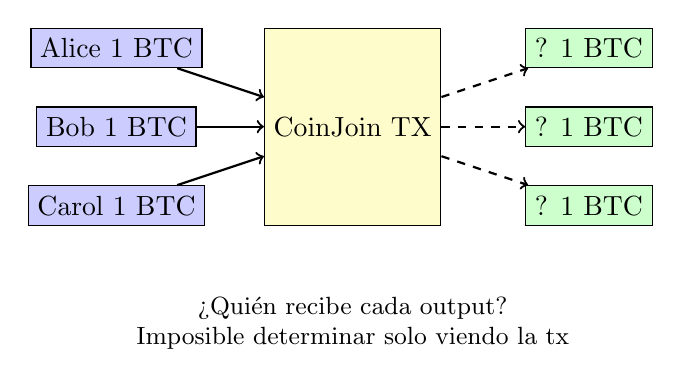
\begin{tikzpicture}[
    node distance=0.8cm,
    input/.style={draw, rectangle, minimum width=1.5cm, minimum height=0.5cm, fill=blue!20},
    output/.style={draw, rectangle, minimum width=1.5cm, minimum height=0.5cm, fill=green!20},
    tx/.style={draw, rectangle, minimum width=2cm, minimum height=2cm, fill=yellow!20},
    arrow/.style={->, thick}
]
    % CoinJoin
    \node[input] (cj_in1) at (0, 1) {Alice 1 BTC};
    \node[input] (cj_in2) at (0, 0) {Bob 1 BTC};
    \node[input] (cj_in3) at (0, -1) {Carol 1 BTC};
    
    \node[tx, minimum height=2.5cm] (cj_tx) at (3, 0) {CoinJoin TX};
    
    \node[output] (cj_out1) at (6, 1) {? 1 BTC};
    \node[output] (cj_out2) at (6, 0) {? 1 BTC};
    \node[output] (cj_out3) at (6, -1) {? 1 BTC};
    
    \draw[arrow] (cj_in1) -- (cj_tx);
    \draw[arrow] (cj_in2) -- (cj_tx);
    \draw[arrow] (cj_in3) -- (cj_tx);
    \draw[arrow, dashed] (cj_tx) -- (cj_out1);
    \draw[arrow, dashed] (cj_tx) -- (cj_out2);
    \draw[arrow, dashed] (cj_tx) -- (cj_out3);
    
    \node at (3, -2.5) [align=center, font=\small] {
        ?`Qui\'en recibe cada output?\\
        Imposible determinar solo viendo la tx
    };
\end{tikzpicture}
\end{center}

\subsection{An\'alisis de Anonimato}

\begin{definition}[Anonymity Set]
El conjunto de posibles or\'igenes/destinos de una transacci\'on. Cuanto mayor el anonymity set, mayor la privacidad.
\[
\text{Anonymity Set} = n \implies \text{Probabilidad de identificaci\'on} = \frac{1}{n}
\]
\end{definition}

\begin{mathnote}
\textbf{Entrop\'ia de Anonimato:}

La entrop\'ia mide la incertidumbre del observador:
\[
H = -\sum_{i=1}^{n} p_i \log_2(p_i)
\]

Para CoinJoin con $n$ participantes equiprobables:
\[
H = -n \cdot \frac{1}{n} \log_2\left(\frac{1}{n}\right) = \log_2(n) \text{ bits}
\]

\begin{center}
\begin{tabular}{cc}
\toprule
Participantes & Entrop\'ia \\
\midrule
2 & 1 bit \\
4 & 2 bits \\
8 & 3 bits \\
16 & 4 bits \\
100 & 6.64 bits \\
\bottomrule
\end{tabular}
\end{center}

Para 128 bits de seguridad, necesitar\'ias $2^{128}$ participantes --- impracticable. Por eso CoinJoin se hace m\'ultiples veces (remix).
\end{mathnote}

\subsection{Requisitos para CoinJoin Efectivo}

\begin{keyidea}
\textbf{Condiciones para anonimato real:}

\begin{enumerate}
    \item \textbf{Outputs uniformes:} Todos los outputs deben tener el mismo monto
    \begin{itemize}
        \item Si Alice pone 1.23 BTC y hay un output de 1.23 BTC, es obvio que es de Alice
        \item Soluci\'on: ``Equal-output CoinJoin'' con denominaciones fijas (0.1, 0.01 BTC)
    \end{itemize}
    
    \item \textbf{Suficientes participantes:} M\'as participantes = mayor anonymity set
    
    \item \textbf{Sin coordinador malicioso:} El coordinador no debe poder vincular inputs con outputs
    
    \item \textbf{M\'ultiples rondas:} Una ronda da anonimato limitado, m\'ultiples rondas lo multiplican
    
    \item \textbf{Timing uniforme:} Participantes deben entrar/salir en momentos similares
\end{enumerate}
\end{keyidea}

\subsection{Implementaciones de CoinJoin}

\begin{definition}[Wasabi Wallet]
Wallet Bitcoin con CoinJoin integrado usando protocolo WabiSabi:
\begin{itemize}
    \item \textbf{Coordinador centralizado:} Pero no puede vincular (Chaumian blind signatures)
    \item \textbf{Denominaciones variables:} WabiSabi permite outputs de diferentes tama\~nos
    \item \textbf{Fees:} 0.3\% del monto mezclado
    \item \textbf{Participantes:} T\'ipicamente 100-150 por ronda
\end{itemize}
\end{definition}

\begin{definition}[JoinMarket]
Mercado descentralizado para CoinJoin:
\begin{itemize}
    \item \textbf{Makers:} Ofrecen liquidez para CoinJoin, ganan fees
    \item \textbf{Takers:} Pagan fees para mezclarse con makers
    \item \textbf{Sin coordinador central:} P2P entre participantes
    \item \textbf{M\'as privacidad:} Pero menos conveniente
\end{itemize}
\end{definition}

\begin{definition}[Whirlpool (Samourai)]
Implementaci\'on de CoinJoin con \'enfasis en simplicidad:
\begin{itemize}
    \item \textbf{Pools fijos:} 0.5, 0.05, 0.01, 0.001 BTC
    \item \textbf{Zero-link:} Entrada y salida completamente desvinculadas
    \item \textbf{Tx0:} Transacci\'on preparatoria que divide UTXOs
    \item \textbf{Remixing gratuito:} Una vez dentro, remix sin costo adicional
\end{itemize}

\textbf{Nota:} En 2024, los fundadores de Samourai fueron arrestados por cargos de lavado de dinero, afectando la disponibilidad del servicio.
\end{definition}

\subsection{Ataques contra CoinJoin}

\begin{remark}
\textbf{Vectores de ataque:}

\begin{enumerate}
    \item \textbf{Amount correlation:}
    \begin{itemize}
        \item Si los outputs no son uniformes, se pueden vincular por monto
        \item Soluci\'on: Equal-output CoinJoin
    \end{itemize}
    
    \item \textbf{Timing analysis:}
    \begin{itemize}
        \item Observar cu\'ando entran/salen fondos del mixer
        \item Vincular por proximidad temporal
        \item Soluci\'on: Delays aleatorios, m\'ultiples rondas
    \end{itemize}
    
    \item \textbf{Sybil attack:}
    \begin{itemize}
        \item Adversario controla m\'ultiples participantes
        \item Reduce el anonymity set real
        \item Soluci\'on: Fees que hacen Sybil costoso
    \end{itemize}
    
    \item \textbf{Intersection attack:}
    \begin{itemize}
        \item Observar m\'ultiples CoinJoins del mismo usuario
        \item Intersecci\'on de anonymity sets reduce opciones
        \item Soluci\'on: No reusar direcciones, mezclar en diferentes pools
    \end{itemize}
    
    \item \textbf{Dust attack:}
    \begin{itemize}
        \item Enviar peque\~nas cantidades a direcciones conocidas
        \item Si el usuario las gasta junto con fondos mezclados, vincula
        \item Soluci\'on: No gastar dust, UTXOs separados
    \end{itemize}
\end{enumerate}
\end{remark}

\subsection{WabiSabi: CoinJoin Avanzado}

\begin{definition}[WabiSabi]
Protocolo de Wasabi Wallet que permite CoinJoin con montos variables usando credenciales an\'onimas:
\begin{itemize}
    \item \textbf{Keyed Verification Anonymous Credentials (KVAC):} Permite demostrar propiedades sin revelar valores
    \item \textbf{Range proofs:} Prueban que montos est\'an en rango v\'alido
    \item \textbf{Sin denominaci\'on fija:} M\'as flexibilidad, mismo anonimato
\end{itemize}
\end{definition}

\begin{mathnote}
\textbf{C\'omo funciona WabiSabi:}

\textbf{Fase 1 - Registro de inputs:}
\begin{enumerate}
    \item Usuario registra UTXO y recibe credencial por el monto
    \item Credencial est\'a ``cegada'' (coordinador no ve monto espec\'ifico)
\end{enumerate}

\textbf{Fase 2 - Registro de outputs:}
\begin{enumerate}
    \item Usuario presenta credenciales (sin vincular a input)
    \item Prueba que suma de outputs $\leq$ suma de credenciales
    \item Registra direcciones de output
\end{enumerate}

\textbf{Fase 3 - Firma:}
\begin{enumerate}
    \item Coordinador crea transacci\'on
    \item Cada usuario firma sus inputs
    \item Broadcast a la red
\end{enumerate}

La magia est\'a en que el coordinador nunca ve la conexi\'on input$\leftrightarrow$output.
\end{mathnote}

%===========================================
\section{CoinShuffle / CoinShuffle++}
\label{sec:coinshuffle}
%===========================================

\subsection{El Problema del Coordinador}

\begin{intuicion}
En CoinJoin b\'asico, hay un problema: alguien tiene que recolectar las direcciones de output de todos los participantes. Si ese ``coordinador'' es malicioso, puede vincular inputs con outputs.

CoinShuffle resuelve esto: los participantes mezclan las direcciones entre ellos, de forma que \textbf{nadie} (ni siquiera otros participantes) sabe qu\'e direcci\'on pertenece a qui\'en.
\end{intuicion}

\subsection{Protocolo CoinShuffle}

\begin{definition}[CoinShuffle]
Protocolo de mezcla descentralizado usando encriptaci\'on por capas:
\begin{enumerate}
    \item Cada participante tiene un par de claves de encriptaci\'on $(pk_i, sk_i)$
    \item Los mensajes (direcciones de output) se encriptan en capas
    \item Cada participante remueve una capa y reordena aleatoriamente
    \item Al final, las direcciones est\'an mezcladas y nadie sabe de qui\'en es cu\'al
\end{enumerate}
\end{definition}

\begin{mathnote}
\textbf{Protocolo Detallado:}

\textbf{Setup:}
\begin{itemize}
    \item $n$ participantes $P_1, ..., P_n$
    \item Cada uno genera par de claves: $(pk_i, sk_i)$
    \item Orden de participantes acordado: $P_1 \to P_2 \to ... \to P_n$
\end{itemize}

\textbf{Fase 1 - Encriptaci\'on:}

Cada participante $P_i$ encripta su direcci\'on $addr_i$ con las claves p\'ublicas de todos los participantes despu\'es de \'el:
\[
m_i = E_{pk_n}(E_{pk_{n-1}}(...E_{pk_{i+1}}(addr_i)...))
\]

$P_i$ env\'ia $m_i$ a $P_{i+1}$.

\textbf{Fase 2 - Shuffle:}

Cada participante $P_j$ (para $j = 2, ..., n$):
\begin{enumerate}
    \item Recibe lista de mensajes cifrados del anterior
    \item Descifra una capa de cada mensaje usando $sk_j$
    \item Permuta aleatoriamente la lista
    \item Env\'ia al siguiente participante
\end{enumerate}

\textbf{Fase 3 - Output:}

$P_n$ termina con lista de direcciones en claro, pero permutadas aleatoriamente. Nadie sabe qu\'e direcci\'on es de qui\'en.
\end{mathnote}

\subsection{CoinShuffle++}

\begin{definition}[CoinShuffle++]
Versi\'on mejorada de CoinShuffle con:
\begin{itemize}
    \item \textbf{DiceMix:} Protocolo de mezcla m\'as eficiente usando DC-nets
    \item \textbf{Blame protocol mejorado:} Identificar participantes maliciosos
    \item \textbf{Menor latencia:} Menos rondas de comunicaci\'on
    \item \textbf{Resistencia a DoS:} Mejor manejo de participantes que abandonan
\end{itemize}
\end{definition}

%===========================================
\section{Chaumian e-cash}
\label{sec:ecash}
%===========================================

\subsection{Historia y Concepto}

\begin{definition}[e-cash (David Chaum, 1982)]
Sistema de dinero digital an\'onimo donde:
\begin{itemize}
    \item Un \textbf{banco/mint} emite tokens firmados
    \item Los tokens son \textbf{bearer instruments} (quien tiene el token, tiene el valor)
    \item El banco \textbf{no puede vincular} emisi\'on con gasto gracias a blind signatures
\end{itemize}
\end{definition}

\begin{mathnote}
\textbf{Impacto Hist\'orico:}

David Chaum fund\'o DigiCash en 1990, implementando e-cash. El sistema fue t\'ecnicamente exitoso pero fall\'o comercialmente. DigiCash quebr\'o en 1998.

Sin embargo, las ideas de Chaum influyeron directamente en:
\begin{itemize}
    \item Bitcoin (anonimato parcial)
    \item Monero (ring signatures derivadas de trabajos relacionados)
    \item Zcash (zero-knowledge para privacidad)
    \item Y ahora: Fedimint, Cashu (e-cash sobre Bitcoin)
\end{itemize}
\end{mathnote}

\subsection{Blind Signatures}

\begin{definition}[Blind Signature]
Esquema de firma digital donde el firmante no ve el mensaje que firma:
\begin{enumerate}
    \item \textbf{Blind:} Usuario ``ciega'' el mensaje $m$ para obtener $m'$
    \item \textbf{Sign:} Firmante firma $m'$ para obtener $\sigma'$
    \item \textbf{Unblind:} Usuario ``desciega'' $\sigma'$ para obtener firma v\'alida $\sigma$ sobre $m$
\end{enumerate}

El firmante nunca ve $m$, pero $\sigma$ es una firma v\'alida de su clave sobre $m$.
\end{definition}

\begin{mathnote}
\textbf{RSA Blind Signatures:}

Usando RSA con clave p\'ublica $(e, n)$ y privada $d$:

\textbf{Blind:}
\begin{enumerate}
    \item Usuario elige $r$ aleatorio coprimo con $n$
    \item Calcula mensaje cegado: $m' = m \cdot r^e \mod n$
\end{enumerate}

\textbf{Sign:}
\begin{enumerate}
    \item Banco firma: $\sigma' = (m')^d = (m \cdot r^e)^d = m^d \cdot r \mod n$
\end{enumerate}

\textbf{Unblind:}
\begin{enumerate}
    \item Usuario calcula: $\sigma = \sigma' \cdot r^{-1} = m^d \cdot r \cdot r^{-1} = m^d \mod n$
\end{enumerate}

$\sigma = m^d$ es una firma RSA v\'alida sobre $m$, pero el banco nunca vio $m$.
\end{mathnote}

\subsection{Protocolo e-cash Completo}

\begin{center}
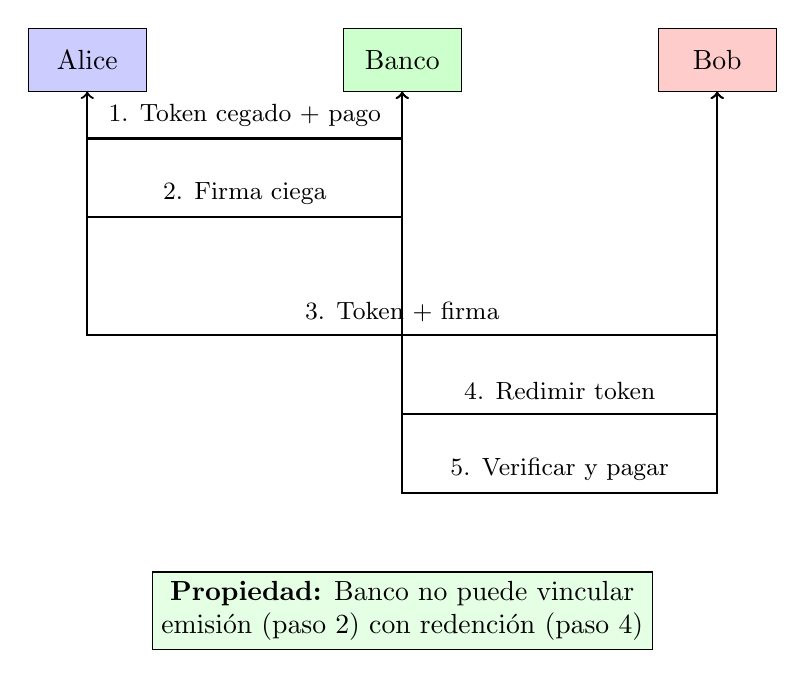
\begin{tikzpicture}[
    node distance=1.5cm,
    actor/.style={draw, rectangle, minimum width=1.5cm, minimum height=0.8cm, align=center},
    arrow/.style={->, thick}
]
    % Actores
    \node[actor, fill=blue!20] (alice) at (0, 0) {Alice};
    \node[actor, fill=green!20] (bank) at (4, 0) {Banco};
    \node[actor, fill=red!20] (bob) at (8, 0) {Bob};
    
    % Fase 1: Emisi\'on
    \draw[arrow] (alice) -- (0, -1) -- (4, -1) -- (bank);
    \node at (2, -0.7) [font=\small] {1. Token cegado + pago};
    
    \draw[arrow] (bank) -- (4, -2) -- (0, -2) -- (alice);
    \node at (2, -1.7) [font=\small] {2. Firma ciega};
    
    % Fase 2: Gasto
    \draw[arrow] (alice) -- (0, -3.5) -- (8, -3.5) -- (bob);
    \node at (4, -3.2) [font=\small] {3. Token + firma};
    
    \draw[arrow] (bob) -- (8, -4.5) -- (4, -4.5) -- (bank);
    \node at (6, -4.2) [font=\small] {4. Redimir token};
    
    \draw[arrow] (bank) -- (4, -5.5) -- (8, -5.5) -- (bob);
    \node at (6, -5.2) [font=\small] {5. Verificar y pagar};
    
    % Propiedad clave
    \node at (4, -7) [draw, rectangle, fill=green!10, align=center] {
        \textbf{Propiedad:} Banco no puede vincular\\
        emisi\'on (paso 2) con redenci\'on (paso 4)
    };
\end{tikzpicture}
\end{center}

\subsection{Prevenci\'on de Doble Gasto}

\begin{remark}
\textbf{El problema:} Un token digital puede ser copiado. ?`C\'omo prevenir que Alice gaste el mismo token dos veces?

\textbf{Soluci\'on centralizada:} El banco mantiene lista de tokens gastados.
\begin{itemize}
    \item Al recibir token, banco verifica que no est\'a en la lista
    \item Si es nuevo, lo a\~nade a la lista y paga
    \item Si est\'a en la lista, rechaza
\end{itemize}

\textbf{Limitaci\'on:} Requiere banco online para cada transacci\'on.
\end{remark}

\subsection{Resurgimiento: Fedimint y Cashu}

\begin{definition}[Fedimint]
E-cash federado construido sobre Bitcoin:
\begin{itemize}
    \item \textbf{Federaci\'on:} M\'ultiples ``guardianes'' controlan los fondos (multisig)
    \item \textbf{Chaumian e-cash:} Tokens ciegos para privacidad dentro de la mint
    \item \textbf{Respaldo Bitcoin:} 1:1 respaldado por BTC en custodia
    \item \textbf{Lightning integration:} Puede recibir/enviar via Lightning
\end{itemize}
\end{definition}

\begin{definition}[Cashu]
Implementaci\'on simple de e-cash sobre Lightning Network:
\begin{itemize}
    \item \textbf{Mint centralizada:} Un operador (m\'as simple que Fedimint)
    \item \textbf{Tokens sobre Lightning:} Dep\'osito/retiro v\'ia Lightning
    \item \textbf{Privacidad local:} Transacciones entre usuarios de la misma mint son privadas
    \item \textbf{Open source:} M\'ultiples implementaciones
\end{itemize}
\end{definition}

\begin{center}
\begin{tabular}{lcc}
\toprule
\textbf{Caracter\'istica} & \textbf{Fedimint} & \textbf{Cashu} \\
\midrule
Custodia & Federada (multisig) & Centralizada \\
Complejidad & Alta & Baja \\
Privacidad & Alta & Alta \\
Resistencia censura & Alta (federaci\'on) & Baja (un operador) \\
Madurez & Beta & Producci\'on \\
Interoperabilidad & Lightning, on-chain & Lightning \\
\bottomrule
\end{tabular}
\end{center}

%===========================================
\section{Dandelion / Dandelion++}
\label{sec:dandelion}
%===========================================

\subsection{El Problema de la Capa de Red}

\begin{intuicion}
Aunque uses CoinJoin o mixing, hay un problema: cuando tu nodo env\'ia una transacci\'on a la red Bitcoin, otros nodos pueden observar \textbf{de d\'onde vino} la transacci\'on.

Si un adversario controla muchos nodos de la red, puede triangular el origen de una transacci\'on bas\'andose en qu\'e nodo la vio primero y cu\'ando.

Dandelion resuelve esto oscureciendo el origen de la transacci\'on a nivel de red.
\end{intuicion}

\begin{definition}[Network-level Deanonymization]
T\'ecnicas para identificar el origen de una transacci\'on observando la red P2P:
\begin{itemize}
    \item \textbf{First-spy estimator:} El nodo que ve la tx primero est\'a cerca del origen
    \item \textbf{Timing analysis:} Patrones temporales de propagaci\'on
    \item \textbf{Spy nodes:} Adversario opera muchos nodos para observar propagaci\'on
\end{itemize}
\end{definition}

\subsection{Protocolo Dandelion}

\begin{definition}[Dandelion]
Protocolo de propagaci\'on en dos fases para ocultar el origen:

\textbf{Fase 1 - Stem (Tallo):}
\begin{itemize}
    \item La tx se propaga en l\'inea, un nodo a la vez
    \item Cada nodo pasa la tx a \textbf{un solo} peer
    \item Duraci\'on: $\sim$10 hops (configurable)
\end{itemize}

\textbf{Fase 2 - Fluff (Pelusa):}
\begin{itemize}
    \item Despu\'es del stem, se hace difusi\'on normal
    \item La tx ya est\'a lejos del origen real
    \item Observadores piensan que el nodo de difusi\'on es el origen
\end{itemize}
\end{definition}

\begin{center}
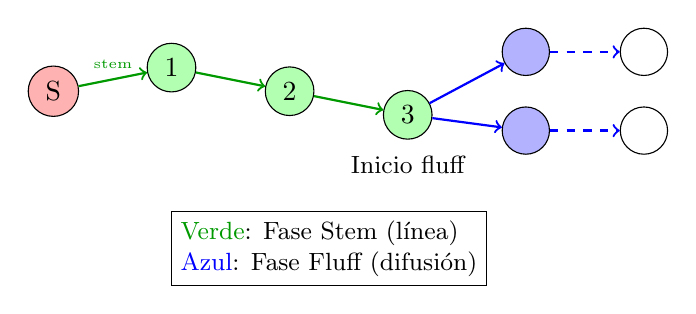
\begin{tikzpicture}[
    node distance=1.5cm,
    peer/.style={draw, circle, minimum size=0.6cm},
    origin/.style={draw, circle, minimum size=0.6cm, fill=red!30},
    stem/.style={draw, circle, minimum size=0.6cm, fill=green!30},
    fluff/.style={draw, circle, minimum size=0.6cm, fill=blue!30},
    arrow_stem/.style={->, thick, green!60!black},
    arrow_fluff/.style={->, thick, blue}
]
    % Red de nodos - Stem phase
    \node[origin] (source) at (0, 0) {S};
    \node[stem] (s1) at (1.5, 0.3) {1};
    \node[stem] (s2) at (3, 0) {2};
    \node[stem] (s3) at (4.5, -0.3) {3};
    
    % Red de nodos - Fluff phase
    \node[fluff] (f1) at (6, 0.5) {};
    \node[fluff] (f2) at (6, -0.5) {};
    \node[peer] (p1) at (7.5, 0.5) {};
    \node[peer] (p2) at (7.5, -0.5) {};
    
    % Stem arrows
    \draw[arrow_stem] (source) -- (s1) node[midway, above] {\tiny stem};
    \draw[arrow_stem] (s1) -- (s2);
    \draw[arrow_stem] (s2) -- (s3);
    
    % Fluff arrows
    \draw[arrow_fluff] (s3) -- (f1);
    \draw[arrow_fluff] (s3) -- (f2);
    \draw[arrow_fluff, dashed] (f1) -- (p1);
    \draw[arrow_fluff, dashed] (f2) -- (p2);
    
    \node at (s3) [below=0.4cm, font=\small] {Inicio fluff};
    
    % Leyenda
    \node[draw, align=left, font=\small] at (3.5, -2) {
        \textcolor{green!60!black}{Verde}: Fase Stem (l\'inea) \\
        \textcolor{blue}{Azul}: Fase Fluff (difusi\'on)
    };
\end{tikzpicture}
\end{center}

\subsection{Dandelion++}

\begin{definition}[Dandelion++]
Versi\'on mejorada de Dandelion que resiste ataques m\'as sofisticados:

\textbf{Mejoras:}
\begin{enumerate}
    \item \textbf{4-regular graph para stem:} Cada nodo tiene exactamente 2 ``outbound stem peers''
    \item \textbf{Decisi\'on per-nodo, no per-tx:} El mismo nodo siempre env\'ia a los mismos stem peers
    \item \textbf{Embargo timer:} Si la tx no se ve en la red despu\'es de un tiempo, hacer fluff
    \item \textbf{Failsafe diffusion:} Evitar que tx se pierda en nodos maliciosos
\end{enumerate}
\end{definition}

%===========================================
\section{Dining Cryptographers Problem (DC-nets)}
\label{sec:dcnets}
%===========================================

\subsection{El Problema Original}

\begin{definition}[Dining Cryptographers Problem (David Chaum, 1988)]
Tres cript\'ografos cenan juntos. Al final, la cuenta est\'a pagada. Quieren saber: ?`pag\'o uno de ellos, o pag\'o la NSA (un tercero)?

Requisitos:
\begin{itemize}
    \item Si uno de ellos pag\'o, los otros no deben saber qui\'en
    \item Si ninguno pag\'o, todos deben saber que fue la NSA
\end{itemize}
\end{definition}

\begin{intuicion}
Es un problema de \textbf{anonimato perfecto}: el que pag\'o quiere decir ``yo pagu\'e'' sin que nadie sepa qui\'en es ``yo''.

La soluci\'on usa XOR y secretos compartidos para crear un canal de comunicaci\'on donde el mensaje aparece ``de la nada'' --- sin revelar qui\'en lo envi\'o.
\end{intuicion}

\subsection{Protocolo DC-net}

\begin{mathnote}
\textbf{Protocolo para 3 participantes:}

\textbf{Setup:}
\begin{itemize}
    \item Cada par de cript\'ografos comparte un bit secreto
    \item $s_{AB}$ entre Alice y Bob
    \item $s_{BC}$ entre Bob y Carol
    \item $s_{AC}$ entre Alice y Carol
\end{itemize}

\textbf{Protocolo:}
\begin{enumerate}
    \item Cada participante XORea sus secretos compartidos
    \item Si quiere enviar ``1'' (yo pagu\'e), tambi\'en XORea con 1
    \item Publica el resultado
\end{enumerate}

Alice calcula: $a = s_{AB} \oplus s_{AC} \oplus m_A$

Bob calcula: $b = s_{AB} \oplus s_{BC} \oplus m_B$

Carol calcula: $c = s_{AC} \oplus s_{BC} \oplus m_C$

\textbf{Verificaci\'on:}
$a \oplus b \oplus c = m_A \oplus m_B \oplus m_C$

Cada secreto aparece dos veces y se cancela. Solo quedan los mensajes.
\end{mathnote}

\begin{remark}
\textbf{Limitaciones de DC-nets:}

\begin{enumerate}
    \item \textbf{Escalabilidad:} $O(n^2)$ secretos compartidos para $n$ participantes
    \item \textbf{Bandwidth:} Cada participante env\'ia $O(n)$ bits por mensaje de 1 bit
    \item \textbf{Disruptors:} Un participante malicioso puede enviar ruido, bloqueando comunicaci\'on
    \item \textbf{Sincronizaci\'on:} Todos deben participar en cada round
    \item \textbf{Setup:} Requiere establecer secretos compartidos de antemano
\end{enumerate}

DC-nets proveen anonimato \textbf{informaci\'on-te\'orico} (perfecto), pero son impr\'actricos a escala. Se usan como base te\'orica para protocolos m\'as pr\'acticos.
\end{remark}

%===========================================
\section{Mix Zones}
\label{sec:mixzones}
%===========================================

\subsection{Contexto: Privacidad de Ubicaci\'on}

\begin{definition}[Location Privacy]
Protecci\'on contra el rastreo de la ubicaci\'on f\'isica de un usuario a trav\'es del tiempo. Amenazas:
\begin{itemize}
    \item \textbf{Tracking:} Seguir movimientos de un individuo
    \item \textbf{Profiling:} Inferir h\'abitos, trabajo, relaciones
    \item \textbf{Correlation:} Vincular identidades en diferentes contextos
\end{itemize}
\end{definition}

\begin{intuicion}
Imagina que llevas un dispositivo GPS que reporta tu ubicaci\'on. Aunque uses pseud\'onimos diferentes, un observador puede vincularlos viendo que ``usuario A'' termina donde ``usuario B'' comienza.

Mix Zones son como ``zonas de cambio de disfraz'': entras como Alice, sales como Bob, y nadie puede vincular Alice con Bob.
\end{intuicion}

\subsection{Concepto de Mix Zone}

\begin{definition}[Mix Zone]
\'Area geogr\'afica donde:
\begin{enumerate}
    \item No hay tracking activo (o est\'a encriptado)
    \item M\'ultiples usuarios entran y salen
    \item Al salir, cada usuario tiene un nuevo pseud\'onimo
    \item Observador no puede vincular entrada con salida
\end{enumerate}
\end{definition}

\begin{center}
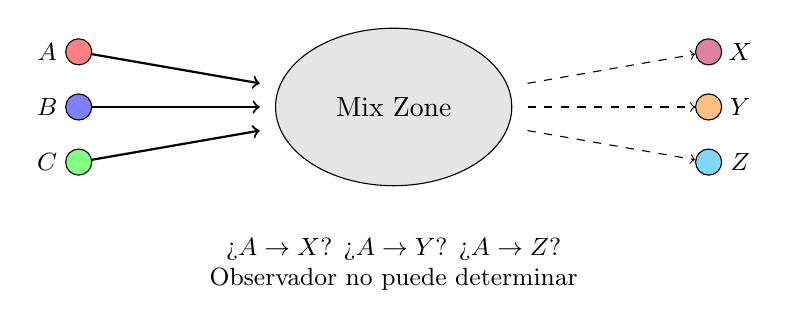
\begin{tikzpicture}[
    node distance=1cm,
    zone/.style={draw, ellipse, minimum width=3cm, minimum height=2cm, fill=gray!20},
    user/.style={draw, circle, minimum size=0.3cm}
]
    % Mix Zone
    \node[zone] (mixzone) at (4, 0) {};
    \node at (4, 0) {Mix Zone};
    
    % Usuarios entrando
    \node[user, fill=red!50] (a_in) at (0, 0.7) {};
    \node[user, fill=blue!50] (b_in) at (0, 0) {};
    \node[user, fill=green!50] (c_in) at (0, -0.7) {};
    
    \node at (-0.4, 0.7) [font=\small] {$A$};
    \node at (-0.4, 0) [font=\small] {$B$};
    \node at (-0.4, -0.7) [font=\small] {$C$};
    
    % Usuarios saliendo - mezclados
    \node[user, fill=purple!50] (x_out) at (8, 0.7) {};
    \node[user, fill=orange!50] (y_out) at (8, 0) {};
    \node[user, fill=cyan!50] (z_out) at (8, -0.7) {};
    
    \node at (8.4, 0.7) [font=\small] {$X$};
    \node at (8.4, 0) [font=\small] {$Y$};
    \node at (8.4, -0.7) [font=\small] {$Z$};
    
    % Flechas
    \draw[->, thick] (a_in) -- (2.3, 0.3);
    \draw[->, thick] (b_in) -- (2.3, 0);
    \draw[->, thick] (c_in) -- (2.3, -0.3);
    
    \draw[->, dashed] (5.7, 0.3) -- (x_out);
    \draw[->, dashed] (5.7, 0) -- (y_out);
    \draw[->, dashed] (5.7, -0.3) -- (z_out);
    
    % Pregunta
    \node at (4, -2) [align=center, font=\small] {
        ?`$A \to X$? ?`$A \to Y$? ?`$A \to Z$?\\
        Observador no puede determinar
    };
\end{tikzpicture}
\end{center}

\subsection{Aplicaciones}

\begin{enumerate}
    \item \textbf{Veh\'iculos conectados:}
    \begin{itemize}
        \item Coches aut\'onomos intercambian datos constantemente
        \item Mix zones en intersecciones, estacionamientos
        \item Cambio de identificadores al salir
    \end{itemize}
    
    \item \textbf{IoT y smart cities:}
    \begin{itemize}
        \item Sensores que rastrean dispositivos (WiFi, Bluetooth)
        \item Zonas designadas donde se cambian identificadores
    \end{itemize}
    
    \item \textbf{Transporte p\'ublico:}
    \begin{itemize}
        \item Estaciones como mix zones naturales
        \item Tarjetas de transporte con pseud\'onimos rotativos
    \end{itemize}
\end{enumerate}

%===========================================
\section{Onion Routing}
\label{sec:onion-routing}
%===========================================

\subsection{Concepto Fundamental}

\begin{definition}[Onion Routing]
T\'ecnica de comunicaci\'on an\'onima donde los mensajes se encriptan en m\'ultiples capas:
\begin{enumerate}
    \item El mensaje se encripta con la clave del \'ultimo nodo (exit)
    \item Se envuelve con la clave del pen\'ultimo nodo
    \item Se envuelve con la clave del primer nodo (entry/guard)
    \item Cada nodo ``pela'' una capa y reenv\'ia al siguiente
    \item Solo el exit node ve el destino final
\end{enumerate}
\end{definition}

\begin{intuicion}
Es como enviar una carta dentro de muchos sobres:
\begin{itemize}
    \item Sobre exterior dice: ``Para Nodo 1''
    \item Nodo 1 abre y ve otro sobre: ``Para Nodo 2''
    \item Nodo 2 abre y ve otro sobre: ``Para Nodo 3''
    \item Nodo 3 abre y ve la carta real con el destino final
\end{itemize}

Ning\'un nodo sabe todo:
\begin{itemize}
    \item Nodo 1 sabe qui\'en envi\'o, pero no el destino
    \item Nodo 3 sabe el destino, pero no qui\'en envi\'o
    \item Nodo 2 no sabe ni origen ni destino
\end{itemize}
\end{intuicion}

\subsection{Arquitectura de Tor}

\begin{definition}[Tor (The Onion Router)]
Red de anonimato m\'as usada, implementando onion routing:
\begin{itemize}
    \item \textbf{Guard nodes:} Primer nodo, conoce IP del usuario
    \item \textbf{Middle nodes:} Nodos intermedios, solo relay
    \item \textbf{Exit nodes:} \'Ultimo nodo, conecta a Internet
    \item \textbf{Directory authorities:} Servidores que listan nodos disponibles
\end{itemize}
\end{definition}

\begin{center}
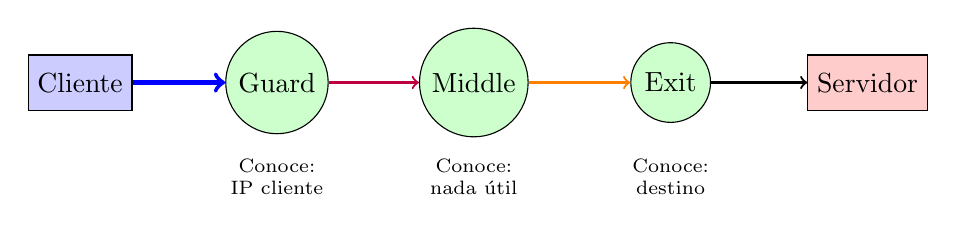
\begin{tikzpicture}[
    node distance=1.5cm,
    client/.style={draw, rectangle, minimum width=1.2cm, minimum height=0.7cm, fill=blue!20},
    tornode/.style={draw, circle, minimum size=0.8cm, fill=green!20},
    server/.style={draw, rectangle, minimum width=1.2cm, minimum height=0.7cm, fill=red!20},
    arrow/.style={->, thick}
]
    % Actores
    \node[client] (client) at (0, 0) {Cliente};
    \node[tornode] (guard) at (2.5, 0) {Guard};
    \node[tornode] (middle) at (5, 0) {Middle};
    \node[tornode] (exit) at (7.5, 0) {Exit};
    \node[server] (server) at (10, 0) {Servidor};
    
    % Conexiones
    \draw[arrow, ultra thick, blue] (client) -- (guard);
    \draw[arrow, thick, purple] (guard) -- (middle);
    \draw[arrow, thick, orange] (middle) -- (exit);
    \draw[arrow] (exit) -- (server);
    
    % Conocimiento de cada nodo
    \node at (2.5, -1.2) [font=\scriptsize, align=center] {Conoce:\\IP cliente};
    \node at (5, -1.2) [font=\scriptsize, align=center] {Conoce:\\nada \'util};
    \node at (7.5, -1.2) [font=\scriptsize, align=center] {Conoce:\\destino};
\end{tikzpicture}
\end{center}

\subsection{Ataques contra Tor}

\begin{remark}
\textbf{Ataques conocidos:}

\begin{enumerate}
    \item \textbf{Traffic correlation:}
    \begin{itemize}
        \item Adversario observa entrada y salida del circuito
        \item Correlaciona por timing y volumen
        \item Efectivo si adversario controla ISPs en ambos extremos
    \end{itemize}
    
    \item \textbf{Sybil attack:}
    \begin{itemize}
        \item Adversario opera muchos nodos
        \item Probabilidad de controlar circuito completo: $(f)^3$ donde $f$ = fracci\'on de nodos
        \item Mitigaci\'on: Guard nodes fijos por usuario
    \end{itemize}
    
    \item \textbf{Website fingerprinting:}
    \begin{itemize}
        \item Patrones de tr\'afico revelan qu\'e sitio se visita
        \item ML puede clasificar con alta precisi\'on
        \item Mitigaci\'on: padding, traffic shaping
    \end{itemize}
    
    \item \textbf{Exit node malicioso:}
    \begin{itemize}
        \item Exit ve tr\'afico no encriptado (HTTP)
        \item Puede modificar contenido, robar credenciales
        \item Mitigaci\'on: Siempre usar HTTPS
    \end{itemize}
\end{enumerate}
\end{remark}

%===========================================
\section{Garlic Routing (I2P)}
\label{sec:garlic-routing}
%===========================================

\subsection{Diferencias con Onion Routing}

\begin{definition}[Garlic Routing]
Variante de onion routing usada en I2P (Invisible Internet Project):
\begin{itemize}
    \item \textbf{Garlic cloves:} M\'ultiples mensajes empaquetados juntos
    \item \textbf{Tunnels unidireccionales:} Separados para entrada y salida
    \item \textbf{Packet-based:} En lugar de stream-based como Tor
    \item \textbf{Red interna:} Optimizado para servicios dentro de I2P
\end{itemize}
\end{definition}

\begin{intuicion}
Si onion routing es una cebolla (capas conc\'entricas), garlic routing es un bulbo de ajo: m\'ultiples ``dientes'' (cloves) empaquetados juntos.

Cada clove puede ir a un destino diferente, lo que dificulta el an\'alisis de tr\'afico.
\end{intuicion}

\subsection{Comparaci\'on Tor vs I2P}

\begin{center}
\small
\begin{tabular}{lcc}
\toprule
\textbf{Caracter\'istica} & \textbf{Tor} & \textbf{I2P} \\
\midrule
Modelo de routing & Onion (circuitos) & Garlic (tunnels) \\
Direccionalidad & Bidireccional & Unidireccional \\
Transporte & Stream (TCP-like) & Packet (UDP-like) \\
Uso principal & Acceso a Internet & Servicios internos \\
Exit nodes & S\'i (a Internet) & Opcional (outproxies) \\
Latencia & Baja-Media & Media-Alta \\
Madurez & Alta (20+ a\~nos) & Media (18+ a\~nos) \\
Usuarios & $\sim$2-3 millones & $\sim$50,000 \\
Servicios ocultos & .onion & .i2p (eepsites) \\
\bottomrule
\end{tabular}
\end{center}

%===========================================
\section{Comparativa de Protocolos}
\label{sec:comparativa-anon}
%===========================================

\begin{center}
\small
\begin{tabular}{lccccc}
\toprule
\textbf{Protocolo} & \textbf{Tipo} & \textbf{Anonimato} & \textbf{Escala} & \textbf{Latencia} & \textbf{Uso} \\
\midrule
CoinJoin & Tx mixing & Computacional & Media & Minutos & Bitcoin \\
CoinShuffle & Tx mixing & Computacional & Media & Minutos & Bitcoin \\
E-cash & Token & Perfecto* & Alta & Segundos & Pagos \\
Dandelion & Red P2P & Heur\'istico & Alta & Segundos & Bitcoin \\
DC-nets & Broadcast & Info-te\'orico & Baja & Alta & Te\'orico \\
Mix Zones & Ubicaci\'on & Computacional & Media & Variable & IoT \\
Tor & Red & Computacional & Alta & Media & Internet \\
I2P & Red & Computacional & Media & Alta & Servicios \\
\bottomrule
\end{tabular}
\end{center}

*E-cash es perfecto dentro de la mint.

%===========================================
\section{Resumen del Cap\'itulo}
\label{sec:resumen-cap6}
%===========================================

\begin{keyidea}
\textbf{Puntos clave de Protocolos de Anonimizaci\'on:}

\textbf{1. CoinJoin:}
\begin{itemize}
    \item Mezcla transacciones de m\'ultiples usuarios en una
    \item Requiere outputs uniformes para efectividad
    \item Implementaciones: Wasabi (WabiSabi), JoinMarket, Whirlpool
    \item Anonymity set limitado por participantes por ronda
\end{itemize}

\textbf{2. CoinShuffle:}
\begin{itemize}
    \item Coordinaci\'on descentralizada para CoinJoin
    \item Usa encriptaci\'on por capas para ocultar direcciones
    \item Nadie (ni otros participantes) sabe qu\'e direcci\'on es de qui\'en
\end{itemize}

\textbf{3. Chaumian E-cash:}
\begin{itemize}
    \item Blind signatures: firmante no ve lo que firma
    \item Tokens bearer: quien tiene el token, tiene el valor
    \item Fedimint: e-cash federado sobre Bitcoin
    \item Cashu: e-cash simple sobre Lightning
\end{itemize}

\textbf{4. Dandelion:}
\begin{itemize}
    \item Oculta origen de transacciones a nivel de red
    \item Fase stem (l\'inea) $\to$ fase fluff (difusi\'on)
    \item Complementa mixing a nivel de transacci\'on
\end{itemize}

\textbf{5. DC-nets:}
\begin{itemize}
    \item Anonimato informaci\'on-te\'orico (perfecto)
    \item XOR de secretos compartidos
    \item Impracticable a escala, base te\'orica
\end{itemize}

\textbf{6. Mix Zones:}
\begin{itemize}
    \item Privacidad de ubicaci\'on
    \item Cambio de pseud\'onimo al atravesar zona
    \item Aplicaciones: veh\'iculos, IoT, transporte
\end{itemize}

\textbf{7. Onion Routing (Tor):}
\begin{itemize}
    \item Encriptaci\'on en capas, cada nodo pela una
    \item 3 hops: Guard, Middle, Exit
    \item Guard conoce IP, Exit conoce destino, ninguno sabe todo
\end{itemize}

\textbf{8. Garlic Routing (I2P):}
\begin{itemize}
    \item M\'ultiples mensajes empaquetados (cloves)
    \item Tunnels unidireccionales
    \item Optimizado para servicios internos (.i2p)
\end{itemize}
\end{keyidea}

\begin{bancozk}
\textbf{Anonimizaci\'on en Banco ZK --- Enfoque Integral:}

Banco ZK combina m\'ultiples t\'ecnicas para privacidad completa:

\begin{center}
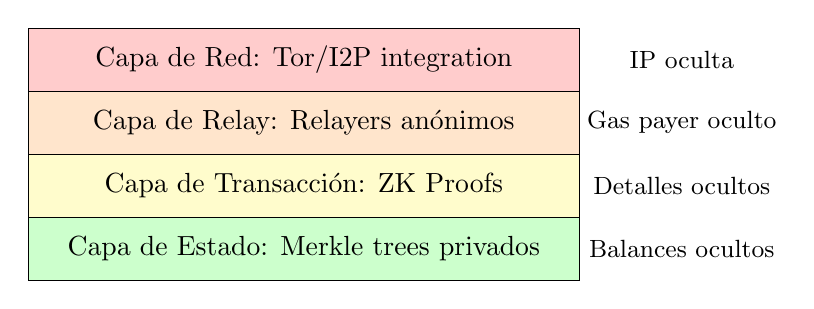
\begin{tikzpicture}[
    layer/.style={draw, rectangle, minimum width=7cm, minimum height=0.8cm, align=center}
]
    \node[layer, fill=red!20] (network) at (0, 2.4) {Capa de Red: Tor/I2P integration};
    \node[layer, fill=orange!20] (relay) at (0, 1.6) {Capa de Relay: Relayers an\'onimos};
    \node[layer, fill=yellow!20] (tx) at (0, 0.8) {Capa de Transacci\'on: ZK Proofs};
    \node[layer, fill=green!20] (state) at (0, 0) {Capa de Estado: Merkle trees privados};
    
    \node at (4.8, 2.4) [font=\small] {IP oculta};
    \node at (4.8, 1.6) [font=\small] {Gas payer oculto};
    \node at (4.8, 0.8) [font=\small] {Detalles ocultos};
    \node at (4.8, 0) [font=\small] {Balances ocultos};
\end{tikzpicture}
\end{center}

\textbf{M\'etricas de privacidad objetivo:}
\begin{itemize}
    \item Anonymity set: Todos los usuarios de Banco ZK ($>$10,000)
    \item Unlinkability: Transacciones no vinculables entre s\'i
    \item Untraceability: Origen de fondos indeterminable
    \item Plausible deniability: No se puede probar participaci\'on
\end{itemize}
\end{bancozk}

\begin{mathnote}
\textbf{M\'etricas de Anonimato:}

\textbf{Anonymity Set Size:}
\[
k\text{-anonymity: cada usuario es indistinguible de al menos } k-1 \text{ otros}
\]

\textbf{Entrop\'ia de Anonimato:}
\[
H = -\sum_{i=1}^{n} p_i \log_2(p_i)
\]

Para distribuci\'on uniforme: $H = \log_2(n)$ bits

\textbf{Anonymity Degree (Diaz et al.):}
\[
d = \frac{H}{H_{max}} = \frac{H}{\log_2(n)}
\]

Donde $d = 1$ es anonimato perfecto, $d = 0$ es identificaci\'on completa.
\end{mathnote}

\begin{keyidea}
\textbf{Principios de Dise\~no para Sistemas An\'onimos:}

\begin{enumerate}
    \item \textbf{Defense in depth:} M\'ultiples capas de protecci\'on
    \item \textbf{Minimize trust:} Reducir puntos de confianza
    \item \textbf{Uniform behavior:} Todos los usuarios se ven iguales
    \item \textbf{Plausible deniability:} No se puede probar participaci\'on
    \item \textbf{Forward secrecy:} Compromiso futuro no afecta pasado
    \item \textbf{Incentive alignment:} Participar debe ser atractivo
    \item \textbf{Graceful degradation:} Fallos parciales no revelan todo
\end{enumerate}
\end{keyidea}

% ============================================
% FIN DEL CAP\'ITULO 6 (CAP 11 ORIGINAL)
% ============================================

% ============================================
% CAP\'ITULO 7: MONEDAS PRIVADAS (PRIVACY COINS)
% (Cap 12 Original $\to$ Cap 7 Vol 2)
% ============================================

\chapter{Monedas Privadas (Privacy Coins)}
\label{ch:monedas-privadas}

\section*{Introducci\'on}

Las privacy coins representan la aplicaci\'on m\'as directa de la criptograf\'ia avanzada para lograr privacidad financiera en blockchain. Este cap\'itulo analiza en profundidad los sistemas m\'as importantes: desde Zcash con sus ZK-SNARKs hasta Monero con ring signatures, y los protocolos de privacidad sobre Ethereum como Tornado Cash, Aztec y Railgun.

\begin{keyidea}
\textbf{Evoluci\'on de la privacidad en criptomonedas:}
\begin{itemize}
    \item \textbf{2009 - Bitcoin:} Pseudonimato (direcciones p\'ublicas, transacciones trazables)
    \item \textbf{2014 - Monero:} Ring signatures para ocultar remitente
    \item \textbf{2016 - Zcash:} ZK-SNARKs para privacidad total
    \item \textbf{2019 - Tornado Cash:} Mixing con ZK sobre Ethereum
    \item \textbf{2022 - Aztec/Railgun:} DeFi privado
    \item \textbf{2023+:} Compliance-friendly privacy (Privacy Pools)
\end{itemize}
\end{keyidea}

\begin{mathnote}
\textbf{Taxonom\'ia de Privacy Coins:}

\textbf{1. Privacidad nativa (Layer 1):}
\begin{itemize}
    \item Zcash: ZK-SNARKs
    \item Monero: Ring signatures + CT
    \item Firo: Lelantus protocol
\end{itemize}

\textbf{2. Privacidad sobre Ethereum (Layer 2/Contracts):}
\begin{itemize}
    \item Tornado Cash: Mixer con SNARKs
    \item Aztec: ZK rollup privado
    \item Railgun: Shielded pool para ERC-20
\end{itemize}

\textbf{3. Privacidad en otros ecosistemas:}
\begin{itemize}
    \item Penumbra: Cosmos/IBC
    \item Namada: Interchain shielded transfers
\end{itemize}
\end{mathnote}

%===========================================
\section{Zcash}
\label{sec:zcash}
%===========================================

\subsection{Historia y Fundamentos}

\begin{definition}[Zcash]
Criptomoneda lanzada en 2016 que implementa transacciones completamente privadas usando ZK-SNARKs:
\begin{itemize}
    \item \textbf{Fundadores:} Zooko Wilcox, basado en protocolo Zerocash
    \item \textbf{Base:} Fork de Bitcoin con adici\'on de transacciones ``shielded''
    \item \textbf{Modelo:} UTXO con ``notes'' encriptadas
    \item \textbf{Dual:} Soporta transacciones transparentes (t-addresses) y privadas (z-addresses)
\end{itemize}
\end{definition}

\begin{mathnote}
\textbf{Timeline de Zcash:}
\begin{itemize}
    \item \textbf{2014:} Zerocash paper publicado
    \item \textbf{2016:} Lanzamiento de Zcash (Sprout)
    \item \textbf{2018:} Upgrade Sapling (mejor performance)
    \item \textbf{2020:} Canopy (eliminaci\'on de founders reward)
    \item \textbf{2022:} NU5 - Orchard (sin trusted setup)
    \item \textbf{2024:} Zcash Shielded Assets (ZSA) en desarrollo
\end{itemize}
\end{mathnote}

\subsection{Arquitectura de Transacciones}

\begin{definition}[Zcash Note]
Una ``note'' en Zcash es el equivalente privado de un UTXO:
\[
\text{note} = (d, pk_d, v, rcm)
\]

Donde:
\begin{itemize}
    \item $d$: Diversifier (permite m\'ultiples direcciones de una clave)
    \item $pk_d$: Clave p\'ublica derivada del diversifier
    \item $v$: Valor (cantidad de ZEC)
    \item $rcm$: Randomness para el commitment
\end{itemize}
\end{definition}

\begin{definition}[Note Commitment]
El commitment a una note se calcula como:
\[
cm = \text{COMMIT}(d, pk_d, v, rcm)
\]

En Sapling: $cm = \text{PedersenHash}(d \| pk_d \| v \| rcm)$

En Orchard: $cm = \text{SinsemillaCommit}(d \| pk_d \| v \| rcm)$

El commitment se a\~nade a un Merkle tree p\'ublico. La note en s\'i permanece encriptada.
\end{definition}

\begin{definition}[Nullifier]
Identificador \'unico que se revela al gastar una note:
\[
nf = \text{PRF}_{nk}(cm)
\]

Donde $nk$ es la nullifier key derivada de la spending key.

\textbf{Propiedades:}
\begin{itemize}
    \item Previene doble gasto: mismo nullifier = misma note gastada
    \item No revela qu\'e note: no se puede vincular $nf$ con $cm$ sin $nk$
\end{itemize}
\end{definition}

\subsection{Sapling (2018)}

\begin{definition}[Sapling]
Segunda generaci\'on de protocolo shielded de Zcash:
\begin{itemize}
    \item \textbf{Sistema de prueba:} Groth16
    \item \textbf{Curva:} BLS12-381
    \item \textbf{Trusted setup:} Powers of Tau + Sapling MPC
    \item \textbf{Performance:} $\sim$40 segundos proving (vs minutos en Sprout)
    \item \textbf{Memoria:} $\sim$40 MB (vs GB en Sprout)
\end{itemize}
\end{definition}

\begin{mathnote}
\textbf{Circuito Sapling Spend:}

El circuito de gasto en Sapling verifica:

\begin{enumerate}
    \item \textbf{Merkle proof:} $cm$ est\'a en el \'arbol con root $rt$
    \[
    \text{MerkleProof}(cm, \text{path}, rt) = 1
    \]
    
    \item \textbf{Nullifier correcto:}
    \[
    nf = \text{PRF}_{nk}^{nf}(\rho)
    \]
    
    \item \textbf{Autorizaci\'on de gasto:}
    \[
    \text{SpendAuthSig.Verify}(ak, m, \sigma) = 1
    \]
    
    \item \textbf{Value commitment:}
    \[
    cv = \text{ValueCommit}(v, rcv)
    \]
\end{enumerate}

\textbf{Inputs p\'ublicos:} $rt$, $nf$, $cv$, $rk$ (randomized key)

\textbf{Inputs privados:} note, path, spending key components
\end{mathnote}

\subsection{Orchard (2022)}

\begin{definition}[Orchard]
Tercera generaci\'on del protocolo shielded, eliminando el trusted setup:
\begin{itemize}
    \item \textbf{Sistema de prueba:} Halo2 (basado en PLONK)
    \item \textbf{Curvas:} Pasta (Pallas y Vesta)
    \item \textbf{Sin trusted setup:} Recursion-friendly
    \item \textbf{Actions:} Unifica spend y output en una sola estructura
    \item \textbf{Performance:} Similar a Sapling pero sin setup
\end{itemize}
\end{definition}

\begin{mathnote}
\textbf{Curvas Pasta:}

Pallas y Vesta son un ``2-cycle'' de curvas el\'ipticas:
\begin{itemize}
    \item $E_p$ (Pallas): $y^2 = x^3 + 5$ sobre $\mathbb{F}_p$
    \item $E_q$ (Vesta): $y^2 = x^3 + 5$ sobre $\mathbb{F}_q$
    \item Propiedad: $|E_p(\mathbb{F}_p)| = q$ y $|E_q(\mathbb{F}_q)| = p$
\end{itemize}

Esta propiedad permite recursi\'on eficiente: una prueba sobre Pallas puede verificarse en un circuito sobre Vesta, y viceversa.
\end{mathnote}

\begin{definition}[Orchard Action]
Un Action combina un spend y un output:
\[
\text{Action} = (\text{spend} \parallel \text{output})
\]

\begin{itemize}
    \item Cada action gasta una note y crea una nueva
    \item Para solo enviar: input es note ``dummy'' de valor 0
    \item Para solo recibir: output es note dummy
    \item Mejora privacidad: no se distingue env\'io de recepci\'on
\end{itemize}
\end{definition}

\subsection{Value Balance y Binding Signature}

\begin{definition}[Value Commitment]
Para ocultar valores pero permitir verificar balance:
\[
cv = v \cdot G_v + rcv \cdot G_{rcv}
\]

Donde:
\begin{itemize}
    \item $v$ es el valor
    \item $rcv$ es randomness
    \item $G_v, G_{rcv}$ son generadores independientes
\end{itemize}

Es un Pedersen commitment que permite verificaci\'on homom\'orfica.
\end{definition}

\begin{mathnote}
\textbf{Verificaci\'on de Balance:}

Para una transacci\'on con inputs $\{v_i\}$ y outputs $\{v_j\}$:

\textbf{Commitments:}
\[
cv_i = v_i \cdot G_v + rcv_i \cdot G_{rcv}
\]
\[
cv_j = v_j \cdot G_v + rcv_j \cdot G_{rcv}
\]

\textbf{Balance check:}
\[
\sum_i cv_i - \sum_j cv_j = \left(\sum_i v_i - \sum_j v_j\right) \cdot G_v + \left(\sum_i rcv_i - \sum_j rcv_j\right) \cdot G_{rcv}
\]

Si los valores balancean ($\sum v_i = \sum v_j + \text{fee}$):
\[
\sum cv_i - \sum cv_j = \text{fee} \cdot G_v + R \cdot G_{rcv}
\]

La binding signature prueba conocimiento de $R = \sum rcv_i - \sum rcv_j$.
\end{mathnote}

\subsection{Claves en Zcash}

\begin{keyidea}
\textbf{Capacidades por nivel de clave:}

\begin{enumerate}
    \item \textbf{Spending Key:}
    \begin{itemize}
        \item Control total: gastar, ver incoming/outgoing
        \item Derivar todas las otras claves
    \end{itemize}
    
    \item \textbf{Full Viewing Key:}
    \begin{itemize}
        \item Ver todas las transacciones (incoming y outgoing)
        \item No puede gastar
        \item \'Util para auditor\'ia, contabilidad
    \end{itemize}
    
    \item \textbf{Incoming Viewing Key:}
    \begin{itemize}
        \item Ver solo transacciones recibidas
        \item No ve a qui\'en enviaste
    \end{itemize}
    
    \item \textbf{Address:}
    \begin{itemize}
        \item Solo permite recibir fondos
        \item Diversifiers permiten m\'ultiples direcciones de una clave
    \end{itemize}
\end{enumerate}
\end{keyidea}

%===========================================
\section{Monero}
\label{sec:monero}
%===========================================

\subsection{Filosof\'ia y Dise\~no}

\begin{definition}[Monero]
Criptomoneda lanzada en 2014 con privacidad obligatoria por defecto:
\begin{itemize}
    \item \textbf{Base:} Protocolo CryptoNote (fork de Bytecoin)
    \item \textbf{Privacidad:} Ring signatures + Stealth addresses + Confidential Transactions
    \item \textbf{Moneda:} XMR
    \item \textbf{Filosof\'ia:} ``Financial privacy is a human right''
\end{itemize}
\end{definition}

\begin{center}
\begin{tabular}{lcc}
\toprule
\textbf{Aspecto} & \textbf{Monero} & \textbf{Zcash} \\
\midrule
Criptograf\'ia & Ring signatures & ZK-SNARKs \\
Privacidad & Obligatoria & Opcional \\
Anonymity set & Ring size (16) & Todo el pool shielded \\
Prueba tama\~no & $\sim$1.5 KB & $\sim$200 bytes \\
Setup & No & S\'i (Sapling) / No (Orchard) \\
Escalabilidad & Peor & Mejor \\
\bottomrule
\end{tabular}
\end{center}

\begin{keyidea}
\textbf{Componentes de privacidad en Monero:}

\begin{enumerate}
    \item \textbf{Ring Signatures:} Ocultan \textit{qui\'en} gasta
    \begin{itemize}
        \item El gastador se ``esconde'' entre m\'ultiples outputs p\'ublicos
    \end{itemize}
    
    \item \textbf{Stealth Addresses:} Ocultan \textit{qui\'en} recibe
    \begin{itemize}
        \item One-time addresses por cada transacci\'on
    \end{itemize}
    
    \item \textbf{Confidential Transactions:} Ocultan \textit{cu\'anto}
    \begin{itemize}
        \item Pedersen commitments para montos
        \item Range proofs para garantizar positividad
    \end{itemize}
\end{enumerate}
\end{keyidea}

\subsection{Ring Signatures}

\begin{definition}[Ring Signature]
Firma que puede ser verificada como proveniente de ``alguno de un grupo'', sin revelar cu\'al miembro espec\'ifico firm\'o:
\[
\text{RingSign}(m, \{pk_1, ..., pk_n\}, sk_i) \to \sigma
\]
\[
\text{RingVerify}(m, \{pk_1, ..., pk_n\}, \sigma) \to \{0, 1\}
\]

\textbf{Propiedades:}
\begin{itemize}
    \item \textbf{Correctness:} Firma v\'alida del firmante real
    \item \textbf{Anonymity:} Verificador no puede distinguir qui\'en firm\'o
    \item \textbf{Unforgeability:} No se puede crear firma sin conocer alg\'un $sk_i$
\end{itemize}
\end{definition}

\begin{center}
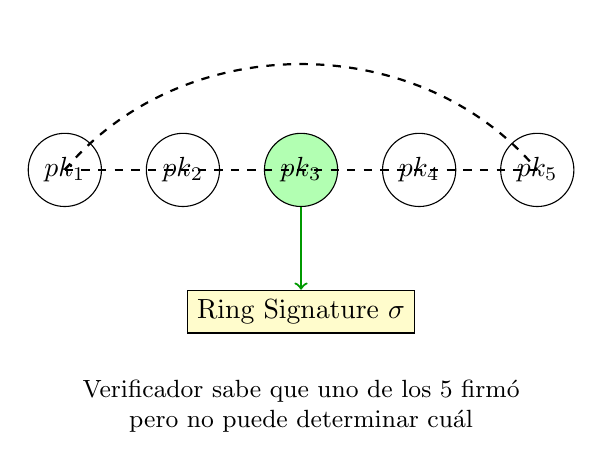
\begin{tikzpicture}[
    node distance=1cm,
    member/.style={draw, circle, minimum size=0.8cm},
    signer/.style={draw, circle, minimum size=0.8cm, fill=green!30}
]
    % Ring members
    \node[member] (m1) at (0, 0) {$pk_1$};
    \node[member] (m2) at (1.5, 0) {$pk_2$};
    \node[signer] (m3) at (3, 0) {$pk_3$};
    \node[member] (m4) at (4.5, 0) {$pk_4$};
    \node[member] (m5) at (6, 0) {$pk_5$};
    
    % Ring visualization
    \draw[thick, dashed] (0, 0) -- (1.5, 0) -- (3, 0) -- (4.5, 0) -- (6, 0);
    \draw[thick, dashed] (0, 0) to[bend left=50] (6, 0);
    
    % Signature
    \node[draw, rectangle, minimum width=2.5cm, fill=yellow!20] (sig) at (3, -1.8) {Ring Signature $\sigma$};
    
    % Arrow from signer
    \draw[->, thick, green!60!black] (m3) -- (sig);
    
    % Note
    \node at (3, -3) [align=center, font=\small] {
        Verificador sabe que uno de los 5 firm\'o\\
        pero no puede determinar cu\'al
    };
\end{tikzpicture}
\end{center}

\begin{definition}[Key Image]
Para prevenir doble gasto sin revelar qu\'e output se gasta:
\[
I = x \cdot H_p(P)
\]

Donde:
\begin{itemize}
    \item $x$ es la clave privada
    \item $P = x \cdot G$ es la clave p\'ublica
    \item $H_p$ es hash-to-point
\end{itemize}

Cada output tiene un \'unico key image. Si el mismo aparece dos veces, es doble gasto.
\end{definition}

\subsection{RingCT (Ring Confidential Transactions)}

\begin{definition}[RingCT]
Combina ring signatures con confidential transactions para ocultar tanto remitente como monto:
\begin{itemize}
    \item \textbf{Introducido:} Enero 2017 (hardfork)
    \item \textbf{Mandatory:} Septiembre 2017
    \item \textbf{Componentes:}
    \begin{enumerate}
        \item MLSAG para firmas de anillo multi-input
        \item Pedersen commitments para montos
        \item Range proofs para probar positividad
    \end{enumerate}
\end{itemize}
\end{definition}

\begin{mathnote}
\textbf{Pedersen Commitment en Monero:}
\[
C = a \cdot G + b \cdot H
\]

Donde:
\begin{itemize}
    \item $a$ es el monto
    \item $b$ es el blinding factor
    \item $G$, $H$ son generadores con relaci\'on desconocida
\end{itemize}

\textbf{Propiedad homom\'orfica:}
\[
C_1 + C_2 = (a_1 + a_2) \cdot G + (b_1 + b_2) \cdot H
\]

Para verificar balance: $\sum C_{inputs} - \sum C_{outputs} = 0 \cdot G + \Delta b \cdot H$
\end{mathnote}

\subsection{Bulletproofs}

\begin{definition}[Bulletproofs]
Sistema de range proofs con tama\~no logar\'itmico:
\begin{itemize}
    \item \textbf{Paper:} B\''unz et al., 2018
    \item \textbf{Tama\~no:} $O(\log n)$ vs $O(n)$ anterior
    \item \textbf{Agregaci\'on:} M\'ultiples range proofs en una
    \item \textbf{Sin trusted setup:} Solo discrete log assumption
\end{itemize}
\end{definition}

\begin{center}
\begin{tabular}{lccc}
\toprule
\textbf{Sistema} & \textbf{Tama\~no (1 output)} & \textbf{Tama\~no (n outputs)} & \textbf{Setup} \\
\midrule
Borromean (original) & 6.2 KB & $n \times 6.2$ KB & No \\
Bulletproofs & 0.7 KB & $0.7 + 0.064 \cdot \log_2 n$ KB & No \\
Bulletproofs+ & 0.6 KB & Similar & No \\
\bottomrule
\end{tabular}
\end{center}

Para una transacci\'on t\'ipica de 2 outputs: Borromean requiere 12.4 KB, Bulletproofs solo 0.8 KB --- un ahorro del 93\%.

\subsection{Stealth Addresses}

\begin{definition}[Stealth Address]
Sistema para generar direcciones \'unicas por transacci\'on:
\begin{enumerate}
    \item Receptor tiene par de claves $(a, A = aG)$ y $(b, B = bG)$
    \item Emisor genera $r$ aleatorio
    \item Calcula: $P = H(rA)G + B$ (one-time key)
    \item Receptor calcula: $P = H(aR)G + B$ donde $R = rG$
    \item Solo receptor puede gastar (conoce $H(aR) + b$)
\end{enumerate}
\end{definition}

%===========================================
\section{Aztec Protocol}
\label{sec:aztec}
%===========================================

\subsection{Visi\'on y Arquitectura}

\begin{definition}[Aztec]
ZK-rollup con privacidad nativa sobre Ethereum:
\begin{itemize}
    \item \textbf{Versi\'on 1 (2020):} Aztec Connect - bridge privado a DeFi
    \item \textbf{Versi\'on 2 (2023+):} Aztec Network - L2 completo con contratos privados
    \item \textbf{Lenguaje:} Noir (DSL para circuitos ZK)
    \item \textbf{Modelo:} UTXO con notes encriptadas
\end{itemize}
\end{definition}

\begin{keyidea}
\textbf{Propuesta de valor de Aztec:}

\begin{enumerate}
    \item \textbf{Privacidad para DeFi existente:}
    \begin{itemize}
        \item Usar Uniswap, Aave, etc. de forma privada
        \item Sin necesidad de que protocolos cambien
    \end{itemize}
    
    \item \textbf{Smart contracts privados:}
    \begin{itemize}
        \item Estado encriptado
        \item L\'ogica verificable sin revelar inputs
        \item Composabilidad entre contratos privados
    \end{itemize}
    
    \item \textbf{Rollup efficiency:}
    \begin{itemize}
        \item Batch proofs para m\'ultiples transacciones
        \item Costos amortizados entre usuarios
    \end{itemize}
\end{enumerate}
\end{keyidea}

\subsection{Noir: Lenguaje para Circuitos Privados}

\begin{definition}[Noir]
Domain-Specific Language (DSL) para escribir programas ZK:
\begin{itemize}
    \item \textbf{Sintaxis:} Similar a Rust
    \item \textbf{Compilaci\'on:} Noir $\to$ ACIR $\to$ Backend proof system
    \item \textbf{Backend-agnostic:} Puede usar diferentes provers
    \item \textbf{Abstracciones:} Alto nivel, oculta complejidad de circuitos
\end{itemize}
\end{definition}

%===========================================
\section{Railgun}
\label{sec:railgun}
%===========================================

\subsection{Concepto: Privacidad para Tokens Existentes}

\begin{definition}[Railgun]
Protocolo de privacidad para cualquier token ERC-20 existente:
\begin{itemize}
    \item \textbf{Sin cambios al token:} Funciona con cualquier ERC-20
    \item \textbf{Shielded pool:} Depositar tokens, transferir privadamente, retirar
    \item \textbf{On Ethereum:} Smart contracts, no L2 separado
    \item \textbf{ZK-SNARKs:} Groth16 para pruebas
\end{itemize}
\end{definition}

\begin{intuicion}
Railgun es como un ``Tornado Cash generalizado'': mientras Tornado Cash solo soporta ETH y algunos tokens espec\'ificos con denominaciones fijas, Railgun soporta cualquier cantidad de cualquier token ERC-20.

Depositas tokens $\to$ entran al pool privado $\to$ transferencias internas son privadas $\to$ retiras a cualquier direcci\'on.
\end{intuicion}

%===========================================
\section{Tornado Cash}
\label{sec:tornado}
%===========================================

\subsection{Historia y Dise\~no}

\begin{definition}[Tornado Cash]
Mixer descentralizado para ETH y tokens ERC-20:
\begin{itemize}
    \item \textbf{Lanzamiento:} 2019
    \item \textbf{Mecanismo:} Shielded pool con denominaciones fijas
    \item \textbf{Tecnolog\'ia:} Groth16 ZK-SNARKs, Circom
    \item \textbf{Estado actual:} Sancionado por OFAC (Agosto 2022)
\end{itemize}
\end{definition}

\begin{remark}
\textbf{Contexto Legal:}

En agosto 2022, el Departamento del Tesoro de EE.UU. (OFAC) sancion\'o las direcciones de Tornado Cash, alegando que fue usado para lavar m\'as de \$7 billones, incluyendo fondos robados por hackers norcoreanos (Lazarus Group).

Esto marc\'o la primera vez que el gobierno sancion\'o c\'odigo (smart contracts) en lugar de personas o empresas. Las implicaciones legales siguen en debate.

\textbf{Nota educativa:} Analizamos Tornado Cash como caso de estudio t\'ecnico, no como recomendaci\'on de uso.
\end{remark}

\subsection{Arquitectura T\'ecnica}

\begin{center}
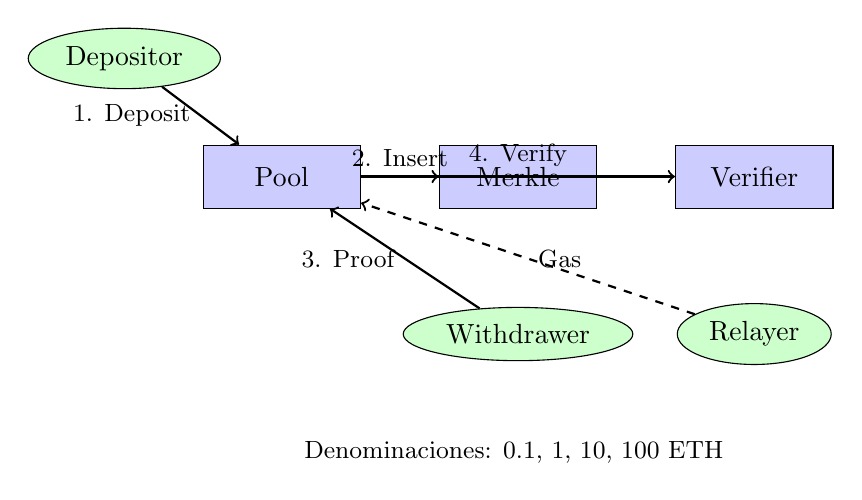
\begin{tikzpicture}[
    node distance=1cm,
    contract/.style={draw, rectangle, minimum width=2cm, minimum height=0.8cm, align=center, fill=blue!20},
    user/.style={draw, ellipse, minimum width=1.2cm, fill=green!20},
    arrow/.style={->, thick}
]
    % Contracts
    \node[contract] (pool) at (0, 0) {Pool};
    \node[contract] (merkle) at (3, 0) {Merkle};
    \node[contract] (verifier) at (6, 0) {Verifier};
    
    % Users
    \node[user] (depositor) at (-2, 1.5) {Depositor};
    \node[user] (withdrawer) at (3, -2) {Withdrawer};
    \node[user] (relayer) at (6, -2) {Relayer};
    
    % Flows
    \draw[arrow] (depositor) -- node[left, font=\small] {1. Deposit} (pool);
    \draw[arrow] (pool) -- node[above, font=\small] {2. Insert} (merkle);
    
    \draw[arrow] (withdrawer) -- node[left, font=\small] {3. Proof} (pool);
    \draw[arrow] (pool) -- node[above, font=\small] {4. Verify} (verifier);
    
    \draw[arrow, dashed] (relayer) -- node[right, font=\small] {Gas} (pool);
    
    % Denominaciones
    \node at (3, -3.5) [align=center, font=\small] {
        Denominaciones: 0.1, 1, 10, 100 ETH
    };
\end{tikzpicture}
\end{center}

\subsection{Relayer Network}

\begin{definition}[Relayer]
Servicio que env\'ia la transacci\'on de withdraw en nombre del usuario:
\begin{itemize}
    \item \textbf{Problema:} Withdraw requiere gas, pero la nueva direcci\'on no tiene ETH
    \item \textbf{Soluci\'on:} Relayer paga gas, cobra fee del monto retirado
    \item \textbf{Privacidad:} Usuario nunca conecta su wallet a la nueva direcci\'on
\end{itemize}
\end{definition}

%===========================================
\section{Umbra (Stealth Payments)}
\label{sec:umbra}
%===========================================

\subsection{Concepto: Privacidad sin ZK}

\begin{definition}[Umbra Protocol]
Sistema de pagos sigilosos (stealth) para Ethereum que no requiere ZK proofs:
\begin{itemize}
    \item \textbf{Mecanismo:} Stealth addresses usando criptograf\'ia de curvas el\'ipticas
    \item \textbf{Ventaja:} Simple, gas-efficient, no requiere proving
    \item \textbf{Limitaci\'on:} Solo oculta receptor, no oculta monto
    \item \textbf{Lanzamiento:} 2021
\end{itemize}
\end{definition}

\begin{intuicion}
El problema: Si Alice quiere recibir pagos, publica su direcci\'on. Cualquiera puede ver todos los pagos que recibe viendo la blockchain.

Soluci\'on de Umbra: Alice publica una ``meta-address'' especial. Cada vez que alguien le paga, genera una direcci\'on \'unica \textit{one-time} que solo Alice puede controlar. Nadie puede vincular estas direcciones a Alice (excepto Alice y el sender).
\end{intuicion}

\subsection{Protocolo de Stealth Addresses}

\begin{mathnote}
\textbf{Stealth Address Generation (ECDH):}

\textbf{Setup:}
\begin{itemize}
    \item Receptor genera dos pares de claves:
    \begin{itemize}
        \item Spending key: $(k_s, K_s = k_s \cdot G)$
        \item Viewing key: $(k_v, K_v = k_v \cdot G)$
    \end{itemize}
    \item Meta-address p\'ublica: $(K_s, K_v)$
\end{itemize}

\textbf{Env\'io (Sender):}
\begin{enumerate}
    \item Genera ephemeral key pair: $(r, R = r \cdot G)$
    \item Calcula shared secret: $S = r \cdot K_v$
    \item Calcula stealth address: $P = K_s + H(S) \cdot G$
    \item Env\'ia fondos a $P$ y publica $R$ on-chain
\end{enumerate}

\textbf{Recepci\'on (Receiver):}
\begin{enumerate}
    \item Escanea blockchain buscando ephemeral keys $R$
    \item Calcula: $S' = k_v \cdot R$ (= $S$ por ECDH)
    \item Calcula stealth address: $P' = K_s + H(S') \cdot G$
    \item Si $P' = P$: el pago es para m\'i
    \item Private key de $P$: $p = k_s + H(S')$
\end{enumerate}
\end{mathnote}

%===========================================
\section{Penumbra}
\label{sec:penumbra}
%===========================================

\begin{definition}[Penumbra]
Blockchain privada en el ecosistema Cosmos con DeFi nativo:
\begin{itemize}
    \item \textbf{Arquitectura:} Zona Cosmos con IBC
    \item \textbf{Privacidad:} Shielded por defecto (como Zcash)
    \item \textbf{DeFi:} DEX privado, staking delegado
    \item \textbf{Viewing keys:} Transparencia selectiva
    \item \textbf{Estado:} Mainnet 2024
\end{itemize}
\end{definition}

\begin{mathnote}
\textbf{Componentes de Penumbra:}

\begin{enumerate}
    \item \textbf{Shielded Pool:}
    \begin{itemize}
        \item Multi-asset (cualquier token IBC)
        \item Notes con commitments (similar a Zcash)
        \item Nullifiers para doble gasto
    \end{itemize}
    
    \item \textbf{DEX (ZSwap):}
    \begin{itemize}
        \item Swaps privados
        \item Concentrated liquidity
        \item Batch auctions para MEV resistance
    \end{itemize}
    
    \item \textbf{Staking:}
    \begin{itemize}
        \item Delegaci\'on privada
        \item Voting shielded
        \item Rewards distribuidos privadamente
    \end{itemize}
    
    \item \textbf{IBC Integration:}
    \begin{itemize}
        \item Transferencias cross-chain
        \item Shielding de tokens de otras cadenas
        \item ``Privacy hub'' del ecosistema
    \end{itemize}
\end{enumerate}
\end{mathnote}

%===========================================
\section{Comparativa de Privacy Coins}
\label{sec:comparativa-privacy}
%===========================================

\begin{center}
\small
\begin{tabular}{lcccccc}
\toprule
\textbf{Sistema} & \textbf{Tipo} & \textbf{Crypto} & \textbf{Setup} & \textbf{Proof} & \textbf{Privacy} \\
\midrule
Zcash Sapling & L1 & Groth16 & S\'i & 200B & Opcional \\
Zcash Orchard & L1 & Halo2 & No & 5KB & Opcional \\
Monero & L1 & Ring+BP & No & 1.5KB & Obligatoria \\
Tornado Cash & Contract & Groth16 & S\'i & 200B & Solo mixing \\
Aztec & L2 & Custom & En dev & Variable & Nativa \\
Railgun & Contract & Groth16 & S\'i & 200B & Shielded pool \\
Umbra & Contract & ECDH & No & N/A & Solo receptor \\
Penumbra & L1 (Cosmos) & Groth16 & S\'i & 200B & Obligatoria \\
\bottomrule
\end{tabular}
\end{center}

\begin{center}
\small
\begin{tabular}{lccccc}
\toprule
\textbf{Sistema} & \textbf{Multi-Asset} & \textbf{DeFi} & \textbf{Compliance} & \textbf{Estado} \\
\midrule
Zcash & Solo ZEC & No & Viewing keys & Producci\'on \\
Monero & Solo XMR & No & Limitado & Producci\'on \\
Tornado Cash & ETH + tokens & No & No & Sancionado \\
Aztec & Cualquier & S\'i & En desarrollo & Testnet \\
Railgun & ERC-20 & Limitado & Privacy Pools & Producci\'on \\
Umbra & ETH + ERC-20 & No & Viewing keys & Producci\'on \\
Penumbra & IBC tokens & DEX, Staking & Viewing keys & Mainnet \\
\bottomrule
\end{tabular}
\end{center}

%===========================================
\section{Resumen del Cap\'itulo}
\label{sec:resumen-cap7}
%===========================================

\begin{keyidea}
\textbf{Puntos clave de Privacy Coins:}

\textbf{1. Zcash:}
\begin{itemize}
    \item Pionero en ZK-SNARKs para privacidad
    \item Sapling (2018): Groth16, trusted setup
    \item Orchard (2022): Halo2, sin trusted setup
    \item Notes, commitments, nullifiers = modelo can\'onico
\end{itemize}

\textbf{2. Monero:}
\begin{itemize}
    \item Ring signatures ocultan remitente
    \item Stealth addresses ocultan receptor
    \item RingCT oculta montos
    \item Bulletproofs para range proofs eficientes
    \item Privacidad obligatoria, mayor anonymity set
\end{itemize}

\textbf{3. Aztec:}
\begin{itemize}
    \item ZK rollup con privacidad nativa
    \item Noir: lenguaje para contratos privados
    \item Permite DeFi privado sobre Ethereum
\end{itemize}

\textbf{4. Railgun:}
\begin{itemize}
    \item Privacy para cualquier ERC-20
    \item Shielded pool con ZK-SNARKs
    \item No requiere cambios a tokens existentes
\end{itemize}

\textbf{5. Tornado Cash:}
\begin{itemize}
    \item Mixer descentralizado para ETH
    \item Denominaciones fijas, simple pero limitado
    \item Sancionado --- lecciones sobre compliance
\end{itemize}

\textbf{6. Umbra:}
\begin{itemize}
    \item Stealth addresses sin ZK
    \item Simple, eficiente en gas
    \item Solo oculta receptor, no monto
\end{itemize}

\textbf{7. Penumbra:}
\begin{itemize}
    \item DeFi privado en Cosmos
    \item IBC para interoperabilidad
    \item Shielded swaps y staking
\end{itemize}
\end{keyidea}

\begin{bancozk}
\textbf{Dise\~no de Banco ZK --- S\'intesis de Privacy Coins:}

Banco ZK incorpora las mejores caracter\'isticas de cada sistema:

\begin{center}
\begin{tabular}{ll}
\toprule
\textbf{Feature} & \textbf{Inspiraci\'on} \\
\midrule
Modelo UTXO con notes & Zcash \\
Nullifiers & Zcash, Tornado \\
Sin trusted setup & Orchard (Halo2) \\
Multi-asset & Railgun, Penumbra \\
DeFi composable & Aztec \\
Relayer network & Tornado Cash \\
Viewing keys & Zcash, Penumbra \\
Privacy Pools (compliance) & Vitalik et al. 2023 \\
\bottomrule
\end{tabular}
\end{center}

\textbf{Arquitectura resultante:}
\begin{enumerate}
    \item \textbf{Base:} L2 sobre Ethereum (seguridad heredada)
    \item \textbf{Privacidad:} Obligatoria por defecto
    \item \textbf{Tokens:} Cualquier ERC-20
    \item \textbf{Proofs:} Halo2 (sin trusted setup)
    \item \textbf{Compliance:} Privacy Pools opcionales
    \item \textbf{DeFi:} AMM privado, lending privado
    \item \textbf{UX:} Relayers para gas, stealth addresses para recepci\'on
\end{enumerate}
\end{bancozk}

% ============================================
% FIN DEL CAP\'ITULO 7 (CAP 12 ORIGINAL)
% ============================================

% ============================================
% CAP\'ITULO 8: T\'ECNICAS DE UNLINKABILITY
% (Cap 13 Original $\to$ Cap 8 Vol 2)
% ============================================

\chapter{T\'ecnicas de Unlinkability}
\label{ch:unlinkability}

\section*{Introducci\'on}

La unlinkability es una propiedad fundamental de los sistemas de privacidad: la imposibilidad de vincular diferentes acciones, transacciones o identidades de un mismo usuario. Este cap\'itulo explora las t\'ecnicas para lograr unlinkability, los ataques que intentan romperla, y las defensas disponibles.

\begin{keyidea}
\textbf{Jerarqu\'ia de privacidad en transacciones:}

\begin{enumerate}
    \item \textbf{Confidencialidad:} Ocultar \textit{qu\'e} se transfiere (montos)
    \item \textbf{Anonimato:} Ocultar \textit{qui\'en} participa (identidades)
    \item \textbf{Unlinkability:} Ocultar \textit{relaciones} entre acciones
    \item \textbf{Unobservability:} Ocultar que \textit{algo ocurri\'o}
\end{enumerate}

Un sistema puede tener anonimato sin unlinkability (pseud\'onimos fijos) o unlinkability sin anonimato (acciones vinculadas a identidad conocida pero no entre s\'i).
\end{keyidea}

\begin{definition}[Unlinkability (Pfitzmann \& Hansen)]
Dos items de inter\'es (IOI) son unlinkable si, desde la perspectiva del atacante, la probabilidad de que est\'en relacionados es igual a la probabilidad a priori (sin informaci\'on adicional).

Formalmente, para items $i_1, i_2$:
\[
P(i_1 \sim i_2 \mid \text{observaci\'on}) = P(i_1 \sim i_2 \mid \text{sin observaci\'on})
\]

Donde $\sim$ denota ``est\'an relacionados''.
\end{definition}

%===========================================
\section{Input/Output Unlinkability}
\label{sec:io-unlinkability}
%===========================================

\subsection{Definici\'on Formal}

\begin{definition}[Input/Output Unlinkability]
En una transacci\'on con m\'ultiples inputs $\{I_1, ..., I_n\}$ y outputs $\{O_1, ..., O_m\}$, input/output unlinkability significa que un observador no puede determinar qu\'e input ``pag\'o'' a qu\'e output con probabilidad mejor que random:
\[
P(I_i \to O_j \mid \text{tx}) = \frac{1}{n \cdot m} \quad \forall i, j
\]
\end{definition}

\begin{mathnote}
\textbf{Niveles de Unlinkability:}

\textbf{Nivel 1 --- Intra-transacci\'on:}
\begin{itemize}
    \item Dentro de una sola transacci\'on
    \item No se puede vincular input espec\'ifico con output espec\'ifico
    \item Ejemplo: CoinJoin con outputs uniformes
\end{itemize}

\textbf{Nivel 2 --- Inter-transacci\'on:}
\begin{itemize}
    \item Entre diferentes transacciones
    \item No se puede rastrear el ``flujo'' de fondos
    \item Ejemplo: Mixer que rompe la cadena de custody
\end{itemize}

\textbf{Nivel 3 --- Con el mundo exterior:}
\begin{itemize}
    \item Entre transacciones on-chain e identidades off-chain
    \item No se puede vincular tx con persona real
    \item Ejemplo: Uso de Tor + direcciones nuevas + timing aleatorio
\end{itemize}
\end{mathnote}

\subsection{M\'etricas de Unlinkability}

\begin{definition}[Anonymity Set]
Conjunto de posibles or\'igenes o destinos de una acci\'on. El tama\~no del anonymity set determina la fortaleza de la unlinkability:
\[
\text{Anonymity Set Size} = |\{x : P(x \text{ es el origen}) > 0\}|
\]
\end{definition}

\begin{definition}[Entrop\'ia de Anonimato]
Medida m\'as precisa que considera las probabilidades:
\[
H = -\sum_{i=1}^{n} p_i \log_2(p_i)
\]

\textbf{Interpretaci\'on:}
\begin{itemize}
    \item $H = 0$: Identificaci\'on completa (un $p_i = 1$)
    \item $H = \log_2(n)$: Anonimato perfecto (todos $p_i = 1/n$)
    \item $0 < H < \log_2(n)$: Anonimato parcial
\end{itemize}
\end{definition}

%===========================================
\section{Transaction Graph Analysis}
\label{sec:graph-analysis}
%===========================================

\subsection{El Grafo de Transacciones}

\begin{definition}[Transaction Graph]
Representaci\'on de la blockchain como grafo dirigido:
\begin{itemize}
    \item \textbf{Nodos:} Transacciones o direcciones
    \item \textbf{Aristas:} Flujo de fondos
    \item \textbf{Peso:} Monto transferido
\end{itemize}

Tipos de grafos:
\begin{enumerate}
    \item \textbf{Transaction graph:} Nodos = txs, aristas = output$\to$input
    \item \textbf{Address graph:} Nodos = direcciones, aristas = pagos
    \item \textbf{Entity graph:} Nodos = entidades (clusters), aristas = relaciones
\end{enumerate}
\end{definition}

\subsection{Heur\'isticas de Clustering}

\begin{definition}[Address Clustering]
T\'ecnicas para agrupar direcciones que probablemente pertenecen a la misma entidad.
\end{definition}

\begin{mathnote}
\textbf{Common Input Ownership Heuristic:}

\textbf{Supuesto:} Si m\'ultiples inputs aparecen en la misma transacci\'on, probablemente pertenecen al mismo due\~no.

\textbf{Raz\'on:} Para firmar una transacci\'on con m\'ultiples inputs, necesitas las claves privadas de todos. Es raro que m\'ultiples personas coordinen para crear una tx.

\textbf{Excepci\'on:} CoinJoin rompe esta heur\'istica intencionalmente.

\textbf{Formalizaci\'on:}
\[
\text{cluster}(a_1) = \text{cluster}(a_2) \text{ si } \exists \text{ tx}: a_1, a_2 \in \text{inputs}(\text{tx})
\]
\end{mathnote}

\begin{mathnote}
\textbf{Change Detection Heuristics:}

El ``change'' (vuelto) de una transacci\'on suele tener caracter\'isticas identificables:

\textbf{H1 --- Direcci\'on nueva:} El change suele ir a una direcci\'on que no exist\'ia antes.

\textbf{H2 --- N\'umero redondo:} Pagos suelen ser n\'umeros redondos (1.0, 0.5, 100). El output ``raro'' (0.0372819) probablemente es change.

\textbf{H3 --- Self-change:} Algunos wallets reusan direcciones de input para change.

\textbf{H4 --- Script type matching:} Change suele usar mismo tipo de script que inputs.
\end{mathnote}

\subsection{Ataques de An\'alisis de Grafos}

\begin{remark}
\textbf{T\'ecnicas avanzadas de deanonimizaci\'on:}

\begin{enumerate}
    \item \textbf{Taint analysis:} Rastrear ``contaminaci\'on'' de fondos desde origen conocido.
    
    \item \textbf{Temporal analysis:} Patrones de timing revelan informaci\'on.
    
    \item \textbf{Value flow analysis:} Seguir montos espec\'ificos a trav\'es del grafo.
    
    \item \textbf{Behavioral clustering:} Patrones de uso similares sugieren misma entidad.
    
    \item \textbf{Cross-chain analysis:} Correlacionar actividad en m\'ultiples blockchains.
\end{enumerate}
\end{remark}

\begin{bancozk}
\textbf{Defensa contra Graph Analysis en Banco ZK:}

Banco ZK es inherentemente resistente a graph analysis porque:

\begin{enumerate}
    \item \textbf{Sin grafo p\'ublico:}
    \begin{itemize}
        \item Las transacciones no revelan remitente ni receptor
        \item Solo se publican nullifiers y commitments
        \item No hay ``aristas'' visibles entre transacciones
    \end{itemize}
    
    \item \textbf{Modelo Note (no UTXO ni Account):}
    \begin{itemize}
        \item Las notes son privadas
        \item Nullifiers no revelan qu\'e note se gasta
        \item No se puede construir el grafo de flujo
    \end{itemize}
    
    \item \textbf{Anonymity set = todo el pool:}
    \begin{itemize}
        \item Cualquier note podr\'ia ser cualquier output anterior
        \item No hay clustering posible
    \end{itemize}
\end{enumerate}

\textbf{Puntos d\'ebiles a mitigar:}
\begin{itemize}
    \item Dep\'ositos/retiros son p\'ublicos (boundary del shielded pool)
    \item Timing de deposits$\to$withdrawals puede correlacionarse
    \item Soluci\'on: Delays aleatorios, batching, cover traffic
\end{itemize}
\end{bancozk}

%===========================================
\section{Timing Attacks y Mitigaciones}
\label{sec:timing-attacks}
%===========================================

\subsection{Anatom\'ia de los Timing Attacks}

\begin{definition}[Timing Attack]
Ataque que explota correlaciones temporales para deanonimizar usuarios:
\begin{itemize}
    \item \textbf{Correlaci\'on temporal:} Eventos cercanos en tiempo probablemente relacionados
    \item \textbf{Patrones regulares:} Actividad predecible revela identidad
    \item \textbf{Timing side-channels:} Informaci\'on filtrada por tiempos de respuesta
\end{itemize}
\end{definition}

\subsection{Tipos de Timing Attacks}

\begin{mathnote}
\textbf{Categor\'ias de Timing Attacks:}

\textbf{1. Deposit-Withdraw Correlation:}
\begin{itemize}
    \item Usuario deposita en mixer, retira poco despu\'es
    \item Adversario correlaciona por proximidad temporal
    \item $P(\text{link}) \propto e^{-\lambda \cdot \Delta t}$ donde $\Delta t$ = tiempo entre eventos
\end{itemize}

\textbf{2. Behavioral Patterns:}
\begin{itemize}
    \item Actividad a las mismas horas cada d\'ia
    \item Patrones semanales (ej: siempre los lunes)
    \item Fingerprint basado en distribuci\'on temporal
\end{itemize}

\textbf{3. External Correlation:}
\begin{itemize}
    \item Withdraw seguido de dep\'osito en exchange
    \item Compra online correlacionada con transacci\'on
    \item Eventos de red (IP logging) correlacionados con txs
\end{itemize}

\textbf{4. Network-Level Timing:}
\begin{itemize}
    \item Observar cu\'ando un nodo propaga una tx
    \item First-seen heuristic para identificar origen
    \item Latencia de respuesta revela ubicaci\'on
\end{itemize}
\end{mathnote}

\subsection{Mitigaciones}

\begin{keyidea}
\textbf{T\'ecnicas de mitigaci\'on de timing attacks:}

\begin{enumerate}
    \item \textbf{Random delays:} A\~nadir retardos aleatorios antes de operaciones.
    
    \item \textbf{Batching:} Agrupar transacciones de m\'ultiples usuarios.
    
    \item \textbf{Cover traffic:} Generar transacciones falsas para confundir.
    
    \item \textbf{Constant-time operations:} Operaciones toman mismo tiempo independiente de datos.
\end{enumerate}
\end{keyidea}

%===========================================
\section{Amount Hiding}
\label{sec:amount-hiding}
%===========================================

\subsection{Por Qu\'e Ocultar Montos}

\begin{intuicion}
Los montos son altamente identificables. Si transfieres exactamente 1.23456789 BTC, y luego alguien gasta exactamente esa cantidad, probablemente eres t\'u.

Adem\'as, los montos revelan informaci\'on sensible:
\begin{itemize}
    \item Salarios (pagos regulares de montos espec\'ificos)
    \item Transacciones comerciales (facturas, precios)
    \item Patrimonio (balances totales)
\end{itemize}
\end{intuicion}

\subsection{T\'ecnicas de Amount Hiding}

\begin{definition}[Pedersen Commitment]
Commitment criptogr\'afico que oculta el valor pero permite verificaci\'on:
\[
C = g^v \cdot h^r
\]

Donde:
\begin{itemize}
    \item $v$ = valor a comprometer
    \item $r$ = factor de cegado (randomness)
    \item $g, h$ = generadores del grupo con relaci\'on discreta desconocida
\end{itemize}

\textbf{Propiedades:}
\begin{enumerate}
    \item \textbf{Hiding:} Sin conocer $r$, no se puede determinar $v$
    \item \textbf{Binding:} Conociendo $(v, r)$, no se puede encontrar $(v', r')$ diferente
    \item \textbf{Homom\'orfico:} $C_1 \cdot C_2 = g^{v_1+v_2} \cdot h^{r_1+r_2}$
\end{enumerate}
\end{definition}

\begin{mathnote}
\textbf{Verificaci\'on de Balance con Pedersen:}

Para transacci\'on con inputs $\{v_i\}$ y outputs $\{v_j\}$:

\textbf{Balance check:}
\[
\prod_i C_i = \prod_j C_j \cdot g^{\text{fee}}
\]

Expandiendo:
\[
g^{\sum v_i} h^{\sum r_i} = g^{\sum v_j + \text{fee}} h^{\sum r_j}
\]

Esto requiere $\sum v_i = \sum v_j + \text{fee}$ \textbf{y} $\sum r_i = \sum r_j$.
\end{mathnote}

\begin{definition}[Range Proof]
Prueba de conocimiento cero de que un valor comprometido est\'a en un rango:
\[
\text{RangeProof}(C, v, r) \implies v \in [0, 2^n)
\]

Sin range proofs, alguien podr\'ia crear valor negativo oculto.
\end{definition}

\begin{center}
\begin{tabular}{lccc}
\toprule
\textbf{Sistema} & \textbf{Tama\~no} & \textbf{Verificaci\'on} & \textbf{Agregaci\'on} \\
\midrule
Borromean & $O(n)$ bits & $O(n)$ & No \\
Bulletproofs & $O(\log n)$ & $O(n)$ & S\'i \\
Bulletproofs+ & $O(\log n)$ & $O(n)$ & S\'i, mejor \\
SNARK-based & $O(1)$ & $O(1)$ & Nativo \\
\bottomrule
\end{tabular}
\end{center}

%===========================================
\section{Decoy Selection}
\label{sec:decoy-selection}
%===========================================

\subsection{El Problema de los Decoys}

\begin{definition}[Decoy (Se\~nuelo)]
En sistemas de ring signatures, un decoy es un output p\'ublico incluido en el ``ring'' para confundir a observadores sobre cu\'al es el output realmente gastado.
\begin{itemize}
    \item \textbf{Ring size:} N\'umero total de miembros (real + decoys)
    \item \textbf{Monero actual:} Ring size = 16 (1 real + 15 decoys)
    \item \textbf{Anonymity set efectivo:} Puede ser menor que ring size
\end{itemize}
\end{definition}

\begin{intuicion}
La idea es simple: si gastas el output \#5, incluyes tambi\'en los outputs \#2, \#8, \#12, ... en tu ring. El verificador sabe que uno de ellos se gast\'o, pero no cu\'al.

El problema: si los decoys son ``obviamente falsos'' (muy viejos, ya gastados en otra tx visible, etc.), el anonymity set se reduce.
\end{intuicion}

\subsection{Distribuci\'on Gamma para Decoys}

\begin{definition}[Gamma Distribution para Decoys]
Monero usa una distribuci\'on gamma para seleccionar decoys bas\'andose en su ``edad'':
\[
f(x; \alpha, \beta) = \frac{\beta^\alpha x^{\alpha-1} e^{-\beta x}}{\Gamma(\alpha)}
\]

Par\'ametros calibrados para imitar el comportamiento real de gasto:
\begin{itemize}
    \item $\alpha$ (shape): Controla la forma de la curva
    \item $\beta$ (rate): Controla qu\'e tan r\'apido decae
\end{itemize}
\end{definition}

\subsection{Ataques contra Decoy Selection}

\begin{remark}
\textbf{Ataques conocidos:}

\begin{enumerate}
    \item \textbf{Temporal analysis:} Si los decoys son de hace a\~nos y el real es de hoy, obvio. Papers han mostrado 80\%+ de precisi\'on.
    
    \item \textbf{Spent output detection:} Si un decoy ya fue gastado (key image conocido), eliminarlo reduce el anonymity set.
    
    \item \textbf{Chain reaction:} Si identifico el real en tx A, puedo usarlo para analizar tx B que lo us\'o como decoy.
    
    \item \textbf{Unusual denominations (pre-RingCT):} Si el monto es \'unico, los decoys con otros montos son obvios.
\end{enumerate}
\end{remark}

%===========================================
\section{Modelos de Datos: Note vs UTXO vs Account}
\label{sec:data-models}
%===========================================

\subsection{Comparaci\'on de Modelos}

\begin{definition}[UTXO Model (Bitcoin)]
Transacciones consumen outputs existentes y crean nuevos:
\begin{itemize}
    \item \textbf{Estado:} Set de Unspent Transaction Outputs
    \item \textbf{Transacci\'on:} inputs (referencias a UTXOs) $\to$ outputs (nuevos UTXOs)
    \item \textbf{Privacidad:} Pseud\'onima (graph analysis posible)
\end{itemize}
\end{definition}

\begin{definition}[Account Model (Ethereum)]
Estado global con balances por cuenta:
\begin{itemize}
    \item \textbf{Estado:} Mapping address $\to$ balance
    \item \textbf{Transacci\'on:} Actualiza balances directamente
    \item \textbf{Privacidad:} Baja (todo p\'ublico)
\end{itemize}
\end{definition}

\begin{definition}[Note Model (Zcash, Tornado)]
Variante privada del modelo UTXO:
\begin{itemize}
    \item \textbf{Estado:} Merkle tree de note commitments + set de nullifiers
    \item \textbf{Note:} $(value, owner, randomness)$ encriptada
    \item \textbf{Privacidad:} Alta (valores y owners ocultos)
\end{itemize}
\end{definition}

\begin{center}
\small
\begin{tabular}{lccc}
\toprule
\textbf{Aspecto} & \textbf{UTXO} & \textbf{Account} & \textbf{Note} \\
\midrule
Paralelismo & Alto & Bajo & Alto \\
Privacidad inherente & Baja & Muy baja & Alta \\
Complejidad tx & Media & Baja & Alta \\
Verificaci\'on & Simple & Simple & ZK proof \\
Graph analysis & Posible & F\'acil & Imposible \\
Doble gasto & Check UTXO set & Check nonce & Check nullifier set \\
\bottomrule
\end{tabular}
\end{center}

%===========================================
\section{Shielded Pools}
\label{sec:shielded-pools}
%===========================================

\subsection{Arquitectura de Shielded Pool}

\begin{definition}[Shielded Pool]
Conjunto de fondos donde todas las transacciones internas son privadas:
\begin{itemize}
    \item \textbf{Boundary:} Interfaz entre mundo p\'ublico y privado
    \item \textbf{Interior:} Todas las operaciones son an\'onimas
    \item \textbf{Anonymity Set:} Todos los fondos en el pool
\end{itemize}
\end{definition}

\subsection{Operaciones del Pool}

\begin{definition}[Shield (Deposit)]
Mover fondos del mundo p\'ublico al privado:
\begin{enumerate}
    \item Usuario env\'ia tokens al contrato (p\'ublico)
    \item Genera note con commitment
    \item Commitment se a\~nade al Merkle tree
    \item Fondos ahora son ``an\'onimos''
\end{enumerate}
\end{definition}

\begin{definition}[Unshield (Withdraw)]
Mover fondos del pool al mundo p\'ublico:
\begin{enumerate}
    \item Usuario genera ZK proof de que posee note v\'alida
    \item Revela nullifier (marca note como gastada)
    \item Contrato env\'ia tokens a direcci\'on especificada
\end{enumerate}
\end{definition}

\begin{definition}[Transfer (Shielded)]
Mover fondos dentro del pool:
\begin{enumerate}
    \item Usuario genera ZK proof
    \item Revela nullifiers de inputs
    \item A\~nade commitments de outputs
    \item \textbf{Ning\'un valor ni direcci\'on es visible}
\end{enumerate}
\end{definition}

\begin{bancozk}
\textbf{Shielded Pool de Banco ZK:}

El pool de Banco ZK es la implementaci\'on central del sistema:

\textbf{Caracter\'isticas:}
\begin{itemize}
    \item Multi-token: Soporta cualquier ERC-20
    \item Unified anonymity set: Todos los tokens comparten anonimato
    \item Efficient proofs: Halo2 sin trusted setup
    \item Compliance-ready: Privacy Pools opcionales
\end{itemize}

\textbf{Anonymity set:}
\[
\text{AS}_{\text{Banco ZK}} = \sum_{\text{tokens}} \text{deposits} - \text{withdrawals}
\]

Con target de 10,000+ notes activas para entrop\'ia $> 13$ bits.
\end{bancozk}

%===========================================
\section{Splitting y Merging de Notas}
\label{sec:split-merge}
%===========================================

\subsection{Motivaci\'on}

\begin{definition}[Split (Divisi\'on)]
Dividir una note en m\'ultiples notes m\'as peque\~nas:
\[
\text{Note}(v) \to \text{Note}(v_1) + \text{Note}(v_2) + ... + \text{Note}(v_n)
\]
donde $v = v_1 + v_2 + ... + v_n$
\end{definition}

\begin{definition}[Merge (Consolidaci\'on)]
Combinar m\'ultiples notes en una sola:
\[
\text{Note}(v_1) + \text{Note}(v_2) + ... + \text{Note}(v_n) \to \text{Note}(v)
\]
donde $v = v_1 + v_2 + ... + v_n$
\end{definition}

\subsection{Riesgos de Privacidad}

\begin{remark}
\textbf{Problemas de privacidad en split/merge:}

\begin{enumerate}
    \item \textbf{Temporal correlation:} Si depositas 100 ETH y haces split inmediato, obvio.
    
    \item \textbf{Amount fingerprinting:} Split 100 $\to$ (37, 63): montos espec\'ificos identificables.
    
    \item \textbf{Merge reveals common ownership:} Si mergeas A + B $\to$ C, sabes que A y B ten\'ian mismo due\~no.
    
    \item \textbf{Graph analysis of splits:} \'Arbol de splits puede rastrearse (``peeling attack'').
\end{enumerate}
\end{remark}

\subsection{Estrategias para Preservar Privacidad}

\begin{keyidea}
\textbf{Mejores pr\'acticas para split/merge:}

\begin{enumerate}
    \item \textbf{Usar denominaciones est\'andar:} Split en potencias de 2 o 10: 100 $\to$ 50 + 50, no 100 $\to$ 37 + 63.
    
    \item \textbf{A\~nadir delays:} No hacer split inmediatamente despu\'es de deposit.
    
    \item \textbf{Evitar merge innecesario:} Mejor usar m\'ultiples inputs en transacci\'on que merge previo.
    
    \item \textbf{Batch con otros:} Si el sistema soporta, hacer split/merge en misma tx que otros usuarios.
    
    \item \textbf{Dummy outputs:} A\~nadir outputs de valor 0 para confundir.
\end{enumerate}
\end{keyidea}

%===========================================
\section{Resumen del Cap\'itulo}
\label{sec:resumen-cap8}
%===========================================

\begin{keyidea}
\textbf{Puntos clave de T\'ecnicas de Unlinkability:}

\textbf{1. Fundamentos:}
\begin{itemize}
    \item Unlinkability = imposibilidad de vincular acciones del mismo usuario
    \item Jerarqu\'ia: confidencialidad $\to$ anonimato $\to$ unlinkability $\to$ unobservability
    \item M\'etricas: anonymity set size, entrop\'ia de anonimato
\end{itemize}

\textbf{2. Graph Analysis:}
\begin{itemize}
    \item Heur\'isticas de clustering: common input ownership, change detection
    \item Ataques: taint analysis, temporal analysis, value flow analysis
    \item Defensa ZK: sin grafo p\'ublico, nullifiers no vinculables
\end{itemize}

\textbf{3. Timing Attacks:}
\begin{itemize}
    \item Correlaci\'on deposit-withdraw, patrones comportamentales
    \item Mitigaciones: random delays, batching, cover traffic
\end{itemize}

\textbf{4. Amount Hiding:}
\begin{itemize}
    \item Pedersen commitments con propiedades homom\'orficas
    \item Range proofs para prevenir inflaci\'on oculta
    \item Alternativa: denominaciones fijas (Tornado Cash)
\end{itemize}

\textbf{5. Decoy Selection:}
\begin{itemize}
    \item Distribuci\'on gamma para imitar comportamiento real
    \item Ataques: temporal analysis, chain reaction
    \item ZK approach elimina necesidad de decoys
\end{itemize}

\textbf{6. Modelos de Datos:}
\begin{itemize}
    \item UTXO: paralelizable pero graph analysis posible
    \item Account: simple pero baja privacidad
    \item Note: alta privacidad, requiere ZK proofs
\end{itemize}

\textbf{7. Shielded Pools:}
\begin{itemize}
    \item Shield/Unshield como boundary p\'ublico-privado
    \item Transfers internos completamente privados
    \item Anonymity set = todo el pool
\end{itemize}

\textbf{8. Split/Merge:}
\begin{itemize}
    \item Necesarios pero riesgosos para privacidad
    \item Mejores pr\'acticas: denominaciones est\'andar, delays, batching
\end{itemize}
\end{keyidea}

\begin{bancozk}
\textbf{Unlinkability en Banco ZK --- S\'intesis:}

Banco ZK implementa unlinkability en m\'ultiples capas:

\begin{center}
\begin{tabular}{ll}
\toprule
\textbf{Capa} & \textbf{T\'ecnica} \\
\midrule
Red & Tor/I2P para conexiones \\
Transacci\'on & Notes + nullifiers + ZK proofs \\
Montos & Pedersen commitments con range proofs \\
Timing & Random delays en operaciones \\
Identidad & Anonymous credentials para compliance \\
\bottomrule
\end{tabular}
\end{center}

\textbf{Resultado:} Sistema donde un observador externo no puede:
\begin{itemize}
    \item Vincular dep\'ositos con retiros
    \item Rastrear flujo de fondos dentro del pool
    \item Identificar partes de una transacci\'on
    \item Correlacionar actividad por timing o montos
\end{itemize}

Solo el usuario (con su viewing key) puede ver su propio historial.
\end{bancozk}

% ============================================
% FIN DEL CAP\'ITULO 8 (CAP 13 ORIGINAL)
% ============================================

% ============================================
% CONCLUSI\'ON DEL VOLUMEN 2
% ============================================

\chapter*{Conclusi\'on del Volumen 2}
\addcontentsline{toc}{chapter}{Conclusi\'on del Volumen 2}

Este segundo volumen de la serie \textbf{Banco ZK} ha completado el recorrido por los fundamentos te\'oricos y pr\'acticos necesarios para comprender y construir sistemas de privacidad en blockchain.

\section*{Resumen por Cap\'itulo}

\begin{enumerate}
    \item \textbf{Compromisos y Estructuras:} Pedersen, KZG, Merkle trees, estructuras de datos para ZK.
    
    \item \textbf{Infraestructura ZK:} Oracles, relayers, circuitos eficientes, optimizaciones.
    
    \item \textbf{Privacidad Avanzada:} T\'ecnicas de ZK para transacciones confidenciales.
    
    \item \textbf{DeFi y Aplicaciones:} AMMs privados, lending, bridges cross-chain.
    
    \item \textbf{Avanzado e Investigaci\'on:} FHE, MPC, t\'ecnicas de frontera.
    
    \item \textbf{Protocolos de Anonimizaci\'on:} CoinJoin, Tor, mixers, DC-nets.
    
    \item \textbf{Monedas Privadas:} Zcash, Monero, Aztec, Railgun, Tornado Cash.
    
    \item \textbf{T\'ecnicas de Unlinkability:} Graph analysis, timing attacks, shielded pools.
\end{enumerate}

\section*{El Sistema Banco ZK Completo}

Combinando ambos vol\'umenes, Banco ZK implementa:

\begin{center}
\begin{tabular}{ll}
\toprule
\textbf{Componente} & \textbf{Implementaci\'on} \\
\midrule
Modelo de datos & Notes con commitments Pedersen \\
Privacidad de montos & Value commitments + range proofs \\
Prevenci\'on doble gasto & Nullifiers verificados con ZK \\
Prueba de validez & Halo2 (sin trusted setup) \\
Estructura de estado & Sparse Merkle Tree \\
Multi-asset & Cualquier token ERC-20 \\
DeFi privado & AMM, lending con ZK \\
Compliance & Privacy Pools opcionales \\
Red & Soporte Tor/I2P \\
Identidad & Anonymous credentials + DIDs \\
\bottomrule
\end{tabular}
\end{center}

\section*{M\'etricas del Volumen 2}

\begin{center}
\begin{tabular}{lc}
\toprule
\textbf{M\'etrica} & \textbf{Cantidad} \\
\midrule
Cap\'itulos & 8 \\
Definiciones formales & $\sim$100 \\
Tablas comparativas & $\sim$25 \\
P\'aginas estimadas & $\sim$200 \\
Referencias bibliogr\'aficas & 95 \\
\bottomrule
\end{tabular}
\end{center}

\vspace{1cm}

\begin{center}
\textit{``Privacy is not about having something to hide.}\\
\textit{Privacy is about having the right to choose}\\
\textit{what to reveal about yourself.''}
\end{center}

\cleardoublepage

% ============================================
% BIBLIOGRAF\'IA
% ============================================
\backmatter

\begin{thebibliography}{99}

\bibitem{pedersen} Pedersen, T. P. (1991). \textit{Non-Interactive and Information-Theoretic Secure Verifiable Secret Sharing}. CRYPTO.

\bibitem{kzg} Kate, A., Zaverucha, G., \& Goldberg, I. (2010). \textit{Constant-Size Commitments to Polynomials and Their Applications}. ASIACRYPT.

\bibitem{plonk} Gabizon, A., Williamson, Z., \& Ciobotaru, O. (2019). \textit{PLONK: Permutations over Lagrange-bases for Oecumenical Noninteractive arguments of Knowledge}. IACR ePrint.

\bibitem{plookup} Gabizon, A., \& Williamson, Z. (2020). \textit{plookup: A simplified polynomial protocol for lookup tables}. IACR ePrint.

\bibitem{halo} Bowe, S., Grigg, J., \& Hopwood, D. (2019). \textit{Halo: Recursive Proof Composition without a Trusted Setup}. IACR ePrint.

\bibitem{nova} Kothapalli, A., Setty, S., \& Tzialla, I. (2022). \textit{Nova: Recursive Zero-Knowledge Arguments from Folding Schemes}. CRYPTO.

\bibitem{supernova} Kothapalli, A., \& Setty, S. (2022). \textit{SuperNova: Proving universal machine executions without universal circuits}. IACR ePrint.

\bibitem{bulletproofs} B\''unz, B., Bootle, J., Boneh, D., Poelstra, A., Wuille, P., \& Maxwell, G. (2018). \textit{Bulletproofs: Short Proofs for Confidential Transactions and More}. S\&P.

\bibitem{groth16} Groth, J. (2016). \textit{On the Size of Pairing-based Non-interactive Arguments}. EUROCRYPT.

\bibitem{pasta} Bowe, S., Grigg, J., \& Hopwood, D. (2020). \textit{The Pasta Curves for Halo 2 and Beyond}. ZCash Documentation.

\bibitem{tornado} Pertsev, A., Semenov, R., \& Storm, R. (2019). \textit{Tornado Cash Privacy Solution}. Whitepaper.

\bibitem{privacypools} Buterin, V., et al. (2023). \textit{Blockchain Privacy and Regulatory Compliance: Towards a Practical Equilibrium}. SSRN.

\bibitem{zkevm-types} Buterin, V. (2022). \textit{The different types of ZK-EVMs}. Blog post.

\bibitem{risczero} RISC Zero Team. (2023). \textit{RISC Zero zkVM: Technical Documentation}. \url{https://dev.risczero.com}

\bibitem{sp1} Succinct Labs. (2024). \textit{SP1: A performant, 100\% open-source, contributor-friendly zkVM}. Documentation.

\bibitem{scroll} Scroll Team. (2023). \textit{Scroll: Native zkEVM Layer 2 for Ethereum}. Technical Documentation.

\bibitem{polygon-zkevm} Polygon Team. (2023). \textit{Polygon zkEVM: Technical Documentation}. \url{https://docs.polygon.technology}

% Chapter 3 references

\bibitem{ring-signatures} Rivest, R., Shamir, A., \& Tauman, Y. (2001). \textit{How to Leak a Secret}. ASIACRYPT.

\bibitem{linkable-ring} Liu, J. K., Wei, V. K., \& Wong, D. S. (2004). \textit{Linkable Spontaneous Anonymous Group Signature for Ad Hoc Groups}. ACISP.

\bibitem{cryptonote} van Saberhagen, N. (2012). \textit{CryptoNote v2.0}. Whitepaper.

\bibitem{clsag} Goodell, B., Noether, S., \& RandomRun. (2019). \textit{Concise Linkable Ring Signatures and Forgery Against Adversarial Keys}. IACR ePrint.

\bibitem{triptych} Noether, S. (2020). \textit{Triptych: Logarithmic-sized Linkable Ring Signatures with Applications}. IACR ePrint.

\bibitem{stealth-addresses} Todd, P. (2014). \textit{Stealth Addresses}. Bitcoin Wiki.

\bibitem{eip5564} Wahrst?tter, A., et al. (2022). \textit{EIP-5564: Stealth Address Standard}. Ethereum Improvement Proposals.

\bibitem{umbra} ScopeLift. (2021). \textit{Umbra Protocol: Privacy-preserving stealth payments for Ethereum}. Documentation.

\bibitem{zcash-keys} Electric Coin Company. (2020). \textit{Zcash Protocol Specification: Key Components}. \url{https://zips.z.cash}

\bibitem{chaum-mix} Chaum, D. (1981). \textit{Untraceable Electronic Mail, Return Addresses, and Digital Pseudonyms}. Communications of the ACM.

\bibitem{nym} Nym Technologies. (2021). \textit{Nym Whitepaper}. \url{https://nymtech.net}

\bibitem{tor} Dingledine, R., Mathewson, N., \& Syverson, P. (2004). \textit{Tor: The Second-Generation Onion Router}. USENIX Security.

\bibitem{i2p} I2P Project. (2003). \textit{I2P: The Invisible Internet Project}. Technical Documentation.

\bibitem{yao-mpc} Yao, A. C. (1982). \textit{Protocols for Secure Computations}. FOCS.

\bibitem{shamir-secret} Shamir, A. (1979). \textit{How to Share a Secret}. Communications of the ACM.

\bibitem{garbled-circuits} Yao, A. C. (1986). \textit{How to Generate and Exchange Secrets}. FOCS.

\bibitem{sgx} Intel Corporation. (2016). \textit{Intel Software Guard Extensions Programming Reference}. Intel Developer Zone.

\bibitem{secret-network} Secret Network. (2020). \textit{Secret Network: Privacy-Preserving Smart Contracts}. Documentation.

\bibitem{oasis} Oasis Labs. (2020). \textit{The Oasis Network: A Privacy-First, Decentralized Computing Platform}. Whitepaper.

\bibitem{frost} Komlo, C., \& Goldberg, I. (2020). \textit{FROST: Flexible Round-Optimized Schnorr Threshold Signatures}. SAC.

% Chapter 4 references

\bibitem{uniswap-v2} Adams, H., Zinsmeister, N., \& Robinson, D. (2020). \textit{Uniswap v2 Core}. Whitepaper.

\bibitem{uniswap-v3} Adams, H., et al. (2021). \textit{Uniswap v3 Core}. Whitepaper.

\bibitem{curve} Egorov, M. (2019). \textit{StableSwap - Efficient Mechanism for Stablecoin Liquidity}. Curve Finance Whitepaper.

\bibitem{balancer} Martinelli, F., \& Mushegian, N. (2019). \textit{Balancer: A Non-Custodial Portfolio Manager}. Whitepaper.

\bibitem{compound} Leshner, R., \& Hayes, G. (2019). \textit{Compound: The Money Market Protocol}. Whitepaper.

\bibitem{aave} Aave Team. (2020). \textit{Aave Protocol Whitepaper}. \url{https://aave.com}

\bibitem{chainlink} Ellis, S., Juels, A., \& Nazarov, S. (2017). \textit{ChainLink: A Decentralized Oracle Network}. Whitepaper.

\bibitem{flash-loans} Qin, K., et al. (2021). \textit{Attacking the DeFi Ecosystem with Flash Loans}. FC 2021.

\bibitem{impermanent-loss} Pintail. (2019). \textit{Uniswap: A Good Deal for Liquidity Providers?}. Medium.

\bibitem{succinct} Succinct Labs. (2023). \textit{SP1: A zkVM for Ethereum}. Documentation.

\bibitem{layerzero} LayerZero Labs. (2021). \textit{LayerZero: Trustless Omnichain Interoperability Protocol}. Whitepaper.

\bibitem{ibc} Kwon, J., \& Buchman, E. (2019). \textit{The Inter-Blockchain Communication Protocol}. Cosmos Documentation.

\bibitem{htlc} Herlihy, M. (2018). \textit{Atomic Cross-Chain Swaps}. PODC.

\bibitem{zkml-ezkl} EZKL Team. (2023). \textit{EZKL: Easy Zero-Knowledge Machine Learning}. Documentation.

% Chapter 5 references

\bibitem{worldcoin} Worldcoin Team. (2023). \textit{Worldcoin: Privacy-Preserving Proof of Personhood}. Whitepaper.

\bibitem{giza} Giza Team. (2023). \textit{Giza: Verifiable Machine Learning on StarkNet}. Documentation.

\bibitem{circomspect} Trail of Bits. (2022). \textit{Circomspect: A Static Analyzer for Circom}. GitHub.

\bibitem{picus} Picus Team. (2023). \textit{Picus: Automated Under-Constraint Detection for ZK Circuits}. IACR ePrint.

\bibitem{ecne} Ecne Team. (2022). \textit{Ecne: Automated Verification of ZK Circuits}. Documentation.

\bibitem{plonky2} Polygon Zero Team. (2022). \textit{Plonky2: Fast Recursive Arguments with PLONK and FRI}. Documentation.

\bibitem{plonky3} Polygon Zero Team. (2023). \textit{Plonky3: Next Generation ZK Proving System}. Documentation.

\bibitem{snarkpack} B\''unz, B., et al. (2021). \textit{SnarkPack: Practical SNARK Aggregation}. FC 2022.

\bibitem{mina} Mina Foundation. (2021). \textit{Mina Protocol: A Succinct Blockchain}. Whitepaper.

\bibitem{nova-paper} Kothapalli, A., Setty, S., \& Tzialla, I. (2022). \textit{Nova: Recursive Zero-Knowledge Arguments from Folding Schemes}. CRYPTO.

\bibitem{supernova-paper} Kothapalli, A., \& Setty, S. (2022). \textit{SuperNova: Proving Universal Machine Executions}. IACR ePrint.

\bibitem{hypernova} Kothapalli, A., \& Setty, S. (2023). \textit{HyperNova: Recursive Arguments from Multilinear IOP}. IACR ePrint.

\bibitem{shor} Shor, P. (1994). \textit{Algorithms for Quantum Computation}. FOCS.

\bibitem{grover} Grover, L. (1996). \textit{A Fast Quantum Mechanical Algorithm for Database Search}. STOC.

\bibitem{nist-pq} NIST. (2024). \textit{Post-Quantum Cryptography Standardization}. NIST.

\bibitem{labrador} Albrecht, M., et al. (2023). \textit{LaBRADOR: Lattice-Based SNARKs}. IACR ePrint.

% Chapter 6 references

\bibitem{coinjoin} Maxwell, G. (2013). \textit{CoinJoin: Bitcoin Privacy for the Real World}. Bitcoin Forum.

\bibitem{wasabi} zkSNACKs. (2018). \textit{Wasabi Wallet: Privacy-Focused Bitcoin Wallet}. Documentation.

\bibitem{wabisabi} Ficsor, A., et al. (2021). \textit{WabiSabi: Centrally Coordinated CoinJoins with Variable Amounts}. IACR ePrint.

\bibitem{joinmarket} JoinMarket Team. (2015). \textit{JoinMarket: Decentralized Bitcoin CoinJoin Implementation}. GitHub.

\bibitem{coinshuffle} Ruffing, T., et al. (2014). \textit{CoinShuffle: Practical Decentralized Coin Mixing for Bitcoin}. ESORICS.

\bibitem{coinshuffle++} Ruffing, T., et al. (2017). \textit{CoinShuffle++: Efficient Decentralized Mixing}. NDSS.

\bibitem{chaum-ecash} Chaum, D. (1982). \textit{Blind Signatures for Untraceable Payments}. CRYPTO.

\bibitem{fedimint} Fedimint Team. (2022). \textit{Fedimint: Federated E-Cash on Bitcoin}. Documentation.

\bibitem{cashu} Cashu Team. (2022). \textit{Cashu: Chaumian E-Cash System for Bitcoin}. Documentation.

\bibitem{dandelion} Venkatakrishnan, S., et al. (2017). \textit{Dandelion: Redesigning the Bitcoin Network for Anonymity}. SIGMETRICS.

\bibitem{dandelion++} Fanti, G., et al. (2018). \textit{Dandelion++: Lightweight Cryptocurrency Networking}. SIGMETRICS.

\bibitem{dcnets} Chaum, D. (1988). \textit{The Dining Cryptographers Problem}. Journal of Cryptology.

\bibitem{mixzones} Beresford, A., \& Stajano, F. (2003). \textit{Location Privacy in Pervasive Computing}. IEEE Pervasive Computing.

\bibitem{tor} Dingledine, R., Mathewson, N., \& Syverson, P. (2004). \textit{Tor: The Second-Generation Onion Router}. USENIX Security.

\bibitem{i2p} I2P Team. (2003). \textit{I2P: The Invisible Internet Project}. Documentation.

% Chapter 7 references

\bibitem{zcash} Hopwood, D., et al. (2016). \textit{Zcash Protocol Specification}. Electric Coin Company.

\bibitem{sapling} Zcash Team. (2018). \textit{Sapling Protocol Specification}. Electric Coin Company.

\bibitem{orchard} Zcash Team. (2022). \textit{Orchard Protocol Specification}. Electric Coin Company.

\bibitem{monero} van Saberhagen, N. (2013). \textit{CryptoNote v 2.0}. CryptoNote Whitepaper.

\bibitem{ringct} Noether, S., et al. (2016). \textit{Ring Confidential Transactions}. Monero Research Lab.

\bibitem{bulletproofs} B\''unz, B., et al. (2018). \textit{Bulletproofs: Short Proofs for Confidential Transactions}. IEEE S\&P.

\bibitem{clsag} Noether, S., \& Goodell, B. (2020). \textit{CLSAG: A Compact Linkable Spontaneous Anonymous Group Signature}. Monero Research Lab.

\bibitem{aztec} Aztec Team. (2023). \textit{Aztec Protocol Specification}. Aztec Documentation.

\bibitem{noir} Aztec Team. (2023). \textit{Noir: Domain-Specific Language for Zero-Knowledge Proofs}. Documentation.

\bibitem{railgun} Railgun Team. (2021). \textit{Railgun Protocol: Privacy for DeFi}. Whitepaper.

\bibitem{tornado} Tornado Cash Team. (2019). \textit{Tornado Cash: Decentralized Mixer for Ethereum}. Documentation.

\bibitem{umbra} ScopeLift. (2021). \textit{Umbra Protocol: Stealth Addresses for Ethereum}. Documentation.

\bibitem{penumbra} Penumbra Labs. (2023). \textit{Penumbra Protocol Specification}. Documentation.

% Chapter 8 references

\bibitem{pfitzmann} Pfitzmann, A., \& Hansen, M. (2010). \textit{A Terminology for Talking about Privacy by Data Minimization}. TU Dresden.

\bibitem{meiklejohn} Meiklejohn, S., et al. (2013). \textit{A Fistful of Bitcoins: Characterizing Payments Among Men with No Names}. IMC.

\bibitem{reid} Reid, F., \& Harrigan, M. (2013). \textit{An Analysis of Anonymity in the Bitcoin System}. Security and Privacy in Social Networks.

\bibitem{moser} M?ser, M., et al. (2018). \textit{An Empirical Analysis of Traceability in the Monero Blockchain}. PoPETs.

\bibitem{yu} Yu, Z., et al. (2019). \textit{New Empirical Traceability Analysis of CryptoNote-Style Blockchains}. Financial Cryptography.

\bibitem{wijaya} Wijaya, D., et al. (2021). \textit{Monero Ring Attack: Recreating Zero Mixin Transaction Effect}. Trust, Security and Privacy in Computing.

\bibitem{kappos} Kappos, G., et al. (2018). \textit{An Empirical Analysis of Anonymity in Zcash}. USENIX Security.

\bibitem{biryukov} Biryukov, A., \& Tikhomirov, S. (2019). \textit{Deanonymization and Linkability of Cryptocurrency Transactions}. IEEE EuroS\&P.

\end{thebibliography}

\end{document}